%% Beginning of file 'sample63.tex'
%%
%% Modified 2019 June
%%
%% This is a sample manuscript marked up using the
%% AASTeX v6.3 LaTeX 2e macros.
%%
%% AASTeX is now based on Alexey Vikhlinin's emulateapj.cls 
%% (Copyright 2000-2015).  See the classfile for details.

%% AASTeX requires revtex4-1.cls (http://publish.aps.org/revtex4/) and
%% other external packages (latexsym, graphicx, amssymb, longtable, and epsf).
%% All of these external packages should already be present in the modern TeX 
%% distributions.  If not they can also be obtained at www.ctan.org.

%% The first piece of markup in an AASTeX v6.x document is the \documentclass
%% command. LaTeX will ignore any data that comes before this command. The 
%% documentclass can take an optional argument to modify the output style.
%% The command below calls the preprint style which will produce a tightly 
%% typeset, one-column, single-spaced document.  It is the default and thus
%% does not need to be explicitly stated.
%%
%%
%% using aastex version 6.3
\documentclass[twocolumn]{aastex63}


%% The default is a single spaced, 10 point font, single spaced article.
%% There are 5 other style options available via an optional argument. They
%% can be invoked like this:
%%
%% \documentclass[arguments]{aastex63}
%% 
%% where the layout options are:
%%
%%  twocolumn   : two text columns, 10 point font, single spaced article.
%%                This is the most compact and represent the final published
%%                derived PDF copy of the accepted manuscript from the publisher
%%  manuscript  : one text column, 12 point font, double spaced article.
%%  preprint    : one text column, 12 point font, single spaced article.  
%%  preprint2   : two text columns, 12 point font, single spaced article.
%%  modern      : a stylish, single text column, 12 point font, article with
%% 		  wider left and right margins. This uses the Daniel
%% 		  Foreman-Mackey and David Hogg design.
%%  RNAAS       : Preferred style for Research Notes which are by design 
%%                lacking an abstract and brief. DO NOT use \begin{abstract}
%%                and \end{abstract} with this style.
%%
%% Note that you can submit to the AAS Journals in any of these 6 styles.
%%
%% There are other optional arguments one can invoke to allow other stylistic
%% actions. The available options are:
%%
%%   astrosymb    : Loads Astrosymb font and define \astrocommands. 
%%   tighten      : Makes baselineskip slightly smaller, only works with 
%%                  the twocolumn substyle.
%%   times        : uses times font instead of the default
%%   linenumbers  : turn on lineno package.
%%   trackchanges : required to see the revision mark up and print its output
%%   longauthor   : Do not use the more compressed footnote style (default) for 
%%                  the author/collaboration/affiliations. Instead print all
%%                  affiliation information after each name. Creates a much 
%%                  longer author list but may be desirable for short 
%%                  author papers.
%% twocolappendix : make 2 column appendix.
%%   anonymous    : Do not show the authors, affiliations and acknowledgments 
%%                  for dual anonymous review.
%%
%% these can be used in any combination, e.g.
%%
%% \documentclass[twocolumn,linenumbers,trackchanges]{aastex63}
%%
%% AASTeX v6.* now includes \hyperref support. While we have built in specific
%% defaults into the classfile you can manually override them with the
%% \hypersetup command. For example,
%%
%% \hypersetup{linkcolor=red,citecolor=green,filecolor=cyan,urlcolor=magenta}
%%
%% will change the color of the internal links to red, the links to the
%% bibliography to green, the file links to cyan, and the external links to
%% magenta. Additional information on \hyperref options can be found here:
%% https://www.tug.org/applications/hyperref/manual.html#x1-40003
%%
%% Note that in v6.3 "bookmarks" has been changed to "true" in hyperref
%% to improve the accessibility of the compiled pdf file.
%%

%%%%% AUTHORS - PLACE YOUR OWN PACKAGES HERE %%%%%

% Only include extra packages if you really need them. Common packages are:
\usepackage{graphicx}	% Including figure files
\usepackage{amsmath}	% Advanced maths commands
\usepackage{amssymb}	% Extra maths symbols
%\usepackage{float}
\usepackage[normalem]{ulem}
\usepackage{booktabs}	
\usepackage{mathtools}	
%

\usepackage{color}
%\usepackage[dvipsnames]{xcolor}
%\usepackage{pdflscape} %based on guideline https://mirror.hmc.edu/ctan/macros/latex/contrib/mnras/mnras_guide.pdf
%\usepackage{lscape}
%\usepackage{rotating}
\usepackage{acronym}   
\usepackage{xspace}
\usepackage{enumitem} % to make enumerate normal nrs http://ctan.org/pkg/enumitem
\usepackage{calc}% http://ctan.org/pkg/calc
\usepackage[caption=false]{subfig}
%\usepackage{subfig} % to show figures next to each other latex
%\let\captionbox\relax
%\usepackage{graphicx,caption,subcaption,showframe}
%%\captionsetup[figure]{labelsep=space,singlelinecheck=false}
%\captionsetup[subfigure]{justification=centering}


%% If you want to create your own macros, you can do so
%% using \newcommand. Your macros should appear before
%% the \begin{document} command.
%%
\newcommand{\vdag}{(v)^\dagger}
\newcommand\aastex{AAS\TeX}
\newcommand\latex{La\TeX}

%%%%%%%%%%%%%%%%%%%%%%%%


\newcommand{\floor}[1]{\textbf{\textcolor{magenta}{[Floor: #1]}}}
\newcommand{\todo}[1]{\textcolor{red}{[To do: #1]}}
\newcommand{\question}[1]{\textcolor{OliveGreen}{[Question: #1]}}
\newcommand{\edo}[1]{\textcolor{Dandelion}{[Edo: #1]}}


\definecolor{ochre}{rgb}{0.8, 0.47, 0.13}
\newcommand{\OMG}[1]{\textcolor{magenta}{#1}} %Todo/remarks by Alejandro Vigna-Gomez
\usepackage{outlines} % for itemize in itemize
%%\newcommand{\floor}[1]{\textcolor{blue}{#1}} %Todo/remarks by Floor
%commands 
\newcommand\Fiducial{\texttt{Fiducial }}

\newcommand\rate{\mathcal{R}}
\newcommand\COMPAS{{\sc{COMPAS }}}

\newcommand{\standard}{\texttt{standard }}
\newcommand{\pluseq}{\mathrel{+}=}
%-- Constants
%\newcommand\hubbleTimeGyrs{14.6353}
\newcommand{\NEhits}{$N_{\text{T,expl}}$ }
\newcommand{\NE}{$N_{\text{expl}}$ }

\newcommand\hubbleTimeGyrs{14.03}



%BHBH mergers
\newcommand\bhns{BH--NS }
\newcommand\nsbh{NS--BH }
\newcommand\bhnsor{BH--NS or NS--BH } 
\newcommand\bhnsand{BH--NS and NS--BH }
\newcommand\bhnsSingle{BHNS\xspace}

% BNS mergers 
\newcommand\fexplOne{$  35(11) $}
\newcommand\EffExplOne{$ 35(11) $}
\newcommand\EffRefOne{$ 35(11) $}
\newcommand\NxMCOne{$  644  $}
\newcommand\NxAISOne{$ 5 (2) \%  $}
\newcommand\gainOne{$ 811 (297)  / 27688  $}
%\newcommand\UncertOne{$1.89 \, 10^{-5}$}



\newcommand\fexplTwo{$58(30)$}
\newcommand\EffExplTwo{$20(14)$}
\newcommand\EffRefTwo{$8(6)$}
\newcommand\NxMCTwo{$1000$}
\newcommand\NxAISTwo{$ 6 (3) \% $}
\newcommand\gainTwo{$1858 (902) / 39753$}

%BH-NS mergers:
\newcommand\fexplThree{$ 51(14)$}
\newcommand\EffExplThree{$7(7)$}
\newcommand\EffRefThree{$2(3)$}
\newcommand\NxMCThree{$517$}
\newcommand\NxAISThree{$10(3) \%$}
\newcommand\gainThree{$1938(383) / 21930$}

%NSNS mergers
\newcommand\fexplFour{$69(42)$}
\newcommand\EffExplFour{$40(26)$}
\newcommand\EffRefFour{$15(10)$}
\newcommand\NxMCFour{$1240$}
\newcommand\NxAISFour{$6(3) \%$}
\newcommand\gainFour{$2546 (1514) / 51442$}

% BHBH mergers with Mtot > 50Msun
\newcommand\fexplFive{$ 6 (3)$}
\newcommand\EffExplFive{$3(2)$}
\newcommand\EffRefFive{$2(1)$}
\newcommand\NxMCFive{$87$}
\newcommand\NxAISFive{$7(3) \%$}
\newcommand\gainFive{$117(67) / 1487$}

% NSNS mergers with t_coal < 50Myr
\newcommand\fexplSix{$49(32)$}
\newcommand\EffExplSix{$29(19)$}
\newcommand\EffRefSix{$14(9)$}
\newcommand\NxMCSix{$541$}
\newcommand\NxAISSix{$9(6) \%$}
\newcommand\gainSix{$1151(745) / 12653$}

% NSNS mergers with t_coal < 50Myr
\newcommand\fexplSeven{$72(32)$}
\newcommand\EffExplSeven{$35(19)$}
\newcommand\EffRefSeven{$1(1)$}
\newcommand\NxMCSeven{$1513$}
\newcommand\NxAISSeven{$5(2) \%$}
\newcommand\gainSeven{$3007 (1479)  / 80116$}

\newcommand\NtotBinaries{$29 \cdot 10^6$\xspace}
\newcommand\NtotBHNS{1076538}

\newcommand\PercentageA{$3.0\%$\xspace}
\newcommand\PercentageB{$69.4\%$\xspace}
\newcommand\PercentageBnoCE{$4.4\%$\xspace}
\newcommand\PercentageBCE{$7.2\%$\xspace}
\newcommand\PercentageC{$5.1\%$\xspace}
\newcommand\PercentageCCE{$1.0\%$\xspace}
\newcommand\PercentageDCCE{$8.7\%$\xspace}
\newcommand\PercentageOther{$1.3\%$\xspace}

\newcommand\PercentageStable{$77.5\%$\xspace}
\newcommand\PercentageImmediateCE{$8.1\%$\xspace}
\newcommand\nBPSmodels{$10$\xspace}
\newcommand\nMSSFRmodels{$28$\xspace}
%\newcommand{\kms}{\ensuremath{\,\rm{km}\,\rm{s}^{-1}}}
%\newcommand{\msun}{\,\mathrm{M}_\odot}


\newcommand\rateObsBHBH{$210$\xspace}
\newcommand\rateObsBHNS{$7$\xspace}
\newcommand\rateObsNSNS{$1$\xspace}

\newcommand\rateDetBHBH{$25$\xspace}
\newcommand\rateDetBHNS{$28$\xspace}
\newcommand\rateDetNSNS{$38$\xspace}



\newcommand{\monei}{\ensuremath{m_{1,\rm{i}}}\xspace}
\newcommand{\mtwoi}{\ensuremath{m_{2,\rm{i}}}\xspace}
\newcommand{\monef}{\ensuremath{m_{1,\rm{f}}}\xspace}
\newcommand{\mtwof}{\ensuremath{m_{2,\rm{f}}}\xspace}
\newcommand{\ai}{\ensuremath{a_{\rm{i}}}\xspace}
\newcommand{\qi}{\ensuremath{q_{\rm{i}}}\xspace}
\newcommand{\Zi}{\ensuremath{Z_{\rm{i}}}\xspace}
\newcommand{\vk}{\ensuremath{v_{\rm{k}}}\xspace}
\newcommand{\thetak}{\ensuremath{{\theta}_{\rm{k}}}\xspace}
\newcommand{\phik}{\ensuremath{{\phi}_{\rm{k}}}\xspace}
\newcommand{\ei}{\ensuremath{{e}_{\rm{i}}}\xspace}

\newcommand{\Rsun}{\ensuremath{\,\rm{R}_{\odot}}\xspace}
\newcommand{\km}{\ensuremath{\,\rm{km}}\xspace}
\newcommand{\kms}{\ensuremath{\,\rm{km}\,\rm{s}^{-1}}\xspace}
\newcommand{\Msun}{\ensuremath{\,\rm{M}_{\odot}}\xspace}
\newcommand{\Lsun}{\ensuremath{\,\rm{L}_{\odot}}\xspace}
\newcommand{\kpc}{\ensuremath{\,\rm{kpc}}\xspace}
\newcommand{\Zsun}{\ensuremath{\,\rm{Z}_{\odot}}\xspace}


%\newcommand{\fbin}{\ensuremath{f_{\rm{bin}}}}
%\newcommand{\vdag}{(v)^\dagger}
\newcommand{\AU}{\ensuremath{\,\mathrm{AU}}\xspace}
\newcommand{\Myr}{\ensuremath{\,\mathrm{Myr}}\xspace}
\newcommand{\yr}{\ensuremath{\,\mathrm{yr}}\xspace}
\newcommand{\yrs}{\ensuremath{\,\mathrm{yr}}\xspace}
\newcommand{\Myrs}{\ensuremath{\,\mathrm{Myr}}\xspace}
\newcommand{\Gyr}{\ensuremath{\,\mathrm{Gyr}}\xspace}
\newcommand{\Gyrs}{\ensuremath{\,\mathrm{Gyr}}\xspace}
\newcommand{\Kelvin}{\ensuremath{\,\mathrm{K}}\xspace}
\newcommand{\yearmin}{\ensuremath{\,\rm{yr}^{-1}}\xspace}
\newcommand{\MpcminThree}{\ensuremath{\,\rm{Mpc}^{-3}}\xspace}
\newcommand{\GpcminThree}{\ensuremath{\,\rm{Gpc}^{-3}}\xspace}

\newcommand{\Hubblemin}{\ensuremath{\mathcal{H}_0^{-1}}\xspace}
\newcommand{\Hubble}{\ensuremath{\mathcal{H}_0}\xspace}

\newcommand{\MSFR}{\ensuremath{{M}_{\rm{SFR}}}\xspace}
\newcommand{\tdelay}{\ensuremath{{t}_{\rm{delay}}}\xspace}
\newcommand{\tDCO}{\ensuremath{{t}_{\rm{DCO}}}\xspace}
\newcommand{\ts}{\ensuremath{{t}_{\rm{s}}}\xspace}
\newcommand{\tevolve}{\ensuremath{{t}_{\rm{evolve}}}\xspace}
\newcommand{\tform}{\ensuremath{{t}_{\rm{form}}}\xspace}
\newcommand{\tmerger}{\ensuremath{{t}_{\rm{m}}}\xspace}
\newcommand{\tinspiral}{\ensuremath{{t}_{\rm{inspiral}}}\xspace}
\newcommand{\thubble}{\ensuremath{{t}_{\mathcal{H}}}\xspace}
\newcommand{\tdet}{\ensuremath{{t}_{\rm{det}}}\xspace}
\newcommand{\Nform}{\ensuremath{{N}_{\rm{form}}}\xspace}
\newcommand{\Ndet}{\ensuremath{{N}_{\rm{det}}}\xspace}
\newcommand{\Nmerger}{\ensuremath{{N}_{\rm{merger}}}\xspace}

\newcommand{\Pdet}{\ensuremath{{P}_{\rm{det}}}\xspace}
\newcommand{\fbin}{\ensuremath{{f}_{\rm{bin}}}\xspace}





\newcommand{\Mchirp}{\ensuremath{{\mathcal{m}}_{\rm{chirp}}}\xspace}
\newcommand{\Vc}{\ensuremath{{V}_{\rm{c}}}\xspace}
\newcommand{\DL}{\ensuremath{{D}_{\rm{L}}}\xspace}
\newcommand{\Dc}{\ensuremath{{D}_{\rm{c}}}\xspace}
%$M_{\rm{SFR}}$  $t_{\rm{delay}} = t_{\rm{form}}  + t_{\rm{merger}}$
%\ts d \Vc
\newcommand\myeq{\stackrel{\mathclap{\normalfont\mbox{def}}}{=}}
\newcommand*\diff{\mathop{}\!\mathrm{d}}

\newcommand{\CMP}{C20}


% final properties of BHNS mergers:
\newcommand{\mnsf}{\ensuremath{m_{\rm{NS}}}\xspace}
\newcommand{\mbhf}{\ensuremath{m_{\rm{BH}}}\xspace}
\newcommand{\mtotf}{\ensuremath{m_{\rm{tot}}}\xspace}
\newcommand{\mchirpf}{\ensuremath{{\mathcal{M}}_{\rm{c}}}\xspace}
\newcommand{\af}{\ensuremath{a_{\rm{f}}}\xspace}
\newcommand{\qf}{\ensuremath{q_{\rm{f}}}\xspace}
\newcommand{\ef}{\ensuremath{{e}_{\rm{f}}}\xspace}
\newcommand{\chibh}{\ensuremath{{\chi}_{\rm{BH}}}\xspace}





%% MODELS 
\newcommand{\mAzero}{\ensuremath{\rm{A}000}\xspace}
\newcommand{\mAxyz}{\ensuremath{\rm{A}xyz}\xspace}
\newcommand{\mxyz}{\ensuremath{\rm{M}xyz}\xspace}     

\newcommand{\Nmodels}{\ensuremath{336}\xspace}
\newcommand{\NmodelsBPS}{\ensuremath{12}\xspace}
\newcommand{\NmodelsMSSFR}{\ensuremath{28}\xspace}
%%% RATE COMMAND
\newcommand{\RateIntrinsicZero}{\ensuremath{\mathcal{R}_{\rm{m}}^{0}}\xspace}
\newcommand{\RateObserved}{\ensuremath{\mathcal{R}_{\rm{det}}}\xspace}

%%%% RATE VALUES 
  \newcommand{\RateIntrinsicAzeroBHBH}{\ensuremath{70}\xspace} 
\newcommand{\RateIntrinsicAzeroBHNS}{\ensuremath{37}\xspace} 
  \newcommand{\RateIntrinsicAzeroNSNS}{\ensuremath{37}\xspace} 
%
  \newcommand{\RateIntrinsicAzeroBHBHmin}{\ensuremath{20}\xspace} 
    \newcommand{\RateIntrinsicAzeroBHBHmax}{\ensuremath{1510}\xspace} 
    %
\newcommand{\RateIntrinsicAzeroBHNSmin}{\ensuremath{2.6}\xspace} 
\newcommand{\RateIntrinsicAzeroBHNSmax}{\ensuremath{661}\xspace} 
%
  \newcommand{\RateIntrinsicAzeroNSNSmin}{\ensuremath{0.24}\xspace} 
  \newcommand{\RateIntrinsicAzeroNSNSmax}{\ensuremath{459}\xspace} 



\newcommand{\RateObservedAzeroBHBH}{\ensuremath{578}\xspace} 
  \newcommand{\RateObservedAzeroBHNS}{\ensuremath{9}\xspace} 
  \newcommand{\RateObservedAzeroNSNS}{\ensuremath{1.5}\xspace} 

\newcommand{\RateObservedAzeroBHBHmax}{\ensuremath{13277}\xspace} 
  \newcommand{\RateObservedAzeroBHBHmin}{\ensuremath{73}\xspace} 
  
  \newcommand{\RateObservedAzeroBHNSmax}{\ensuremath{132}\xspace} 
    \newcommand{\RateObservedAzeroBHNSmin}{\ensuremath{0.5}\xspace} 
    
  \newcommand{\RateObservedAzeroNSNSmax}{\ensuremath{22}\xspace} 
  \newcommand{\RateObservedAzeroNSNSmin}{\ensuremath{0.02}\xspace} 


%-- abbreviations
%List of abbreviations
\acrodef{GSMF}{galaxy mass function, the number density of galaxies per logarithmic mass bin}
\acrodef{MZR}{mass-metallicity relation}
\acrodef{SFR}{star formation rate}

\acrodef{NSNS}{binary neutron star}
\acrodef{BHBH}{binary black hole}

\acrodef{DCO}{double compact object}
\acrodef{NS}{neutron star}
\acrodef{BH}{black hole}
\acrodef{BH--NS}{black hole-neutron star}
\acrodef{GRB}{gamma--ray burst}
\acrodef{RLOF}{Roche-lobe overflow}
\acrodef{CE}{common envelope}

\acrodef{CE}{common-envelope}
\acrodef{GW}{gravitational wave}
\acrodef{SN}{supernova}
\acrodefplural{SN}[SNe]{supernovae}
\acrodef{ECSN}{electron-capture SN}
\acrodef{PISN}{pair-instability SN}
\acrodefplural{ECSN}[ECSNe]{electron-capture SN}
\acrodef{USSN}{ultra-stripped SN}
\acrodefplural{USSN}[USSNe]{ultra-stripped SN}
\acrodef{CCSN}{core-collapse SN}
\acrodefplural{CCSN}[CCSNe]{core-collapse SN}
\acrodef{COMPAS}{
Compact Object Mergers: Population Astrophysics and Statistics}
\acrodef{MSSFR}{metallicity-specific star formation rate}


%%%%%%%%%%%%%%%%%%%%%%%%


%% Reintroduced the \received and \accepted commands from AASTeX v5.2
\received{XX}
\revised{XX}
\accepted{XX}
%% Command to document which AAS Journal the manuscript was submitted to.
%% Adds "Submitted to " the argument.
\submitjournal{AJ}

%% For manuscript that include authors in collaborations, AASTeX v6.3
%% builds on the \collaboration command to allow greater freedom to 
%% keep the traditional author+affiliation information but only show
%% subsets. The \collaboration command now must appear AFTER the group
%% of authors in the collaboration and it takes TWO arguments. The last
%% is still the collaboration identifier. The text given in this
%% argument is what will be shown in the manuscript. The first argument
%% is the number of author above the \collaboration command to show with
%% the collaboration text. If there are authors that are not part of any
%% collaboration the \nocollaboration command is used. This command takes
%% one argument which is also the number of authors above to show. A
%% dashed line is shown to indicate no collaboration. This example manuscript
%% shows how these commands work to display specific set of authors 
%% on the front page.
%%
%% For manuscript without any need to use \collaboration the 
%% \AuthorCollaborationLimit command from v6.2 can still be used to 
%% show a subset of authors.
%
%\AuthorCollaborationLimit=2
%
%% will only show Schwarz & Muench on the front page of the manuscript
%% (assuming the \collaboration and \nocollaboration commands are
%% commented out).
%%
%% Note that all of the author will be shown in the published article.
%% This feature is meant to be used prior to acceptance to make the
%% front end of a long author article more manageable. Please do not use
%% this functionality for manuscripts with less than 20 authors. Conversely,
%% please do use this when the number of authors exceeds 40.
%%
%% Use \allauthors at the manuscript end to show the full author list.
%% This command should only be used with \AuthorCollaborationLimit is used.

%% The following command can be used to set the latex table counters.  It
%% is needed in this document because it uses a mix of latex tabular and
%% AASTeX deluxetables.  In general it should not be needed.
%\setcounter{table}{1}

%%%%%%%%%%%%%%%%%%%%%%%%%%%%%%%%%%%%%%%%%%%%%%%%%%%%%%%%%%%%%%%%%%%%%%%%%%%%%%%%
%%
%% The following section outlines numerous optional output that
%% can be displayed in the front matter or as running meta-data.
%%
%% If you wish, you may supply running head information, although
%% this information may be modified by the editorial offices.
\shorttitle{Characteristics of BHNS mergers}
\shortauthors{Broekgaarden et al.}
%%
%% You can add a light gray and diagonal water-mark to the first page 
%% with this command:
%% \watermark{text}
%% where "text", e.g. DRAFT, is the text to appear.  If the text is 
%% long you can control the water-mark size with:
%% \setwatermarkfontsize{dimension}
%% where dimension is any recognized LaTeX dimension, e.g. pt, in, etc.
%%
%%%%%%%%%%%%%%%%%%%%%%%%%%%%%%%%%%%%%%%%%%%%%%%%%%%%%%%%%%%%%%%%%%%%%%%%%%%%%%%%

%% This is the end of the preamble.  Indicate the beginning of the
%% manuscript itself with \begin{document}.

\begin{document}

\title{Predictions for  gravitational-wave observations from \bhnsSingle mergers }

%% LaTeX will automatically break titles if they run longer than
%% one line. However, you may use \\ to force a line break if
%% you desire. In v6.3 you can include a footnote in the title.

%% A significant change from earlier AASTEX versions is in the structure for 
%% calling author and affiliations. The change was necessary to implement 
%% auto-indexing of affiliations which prior was a manual process that could 
%% easily be tedious in large author manuscripts.
%%
%% The \author command is the same as before except it now takes an optional
%% argument which is the 16 digit ORCID. The syntax is:
%% \author[xxxx-xxxx-xxxx-xxxx]{Author Name}
%%
%% This will hyperlink the author name to the author's ORCID page. Note that
%% during compilation, LaTeX will do some limited checking of the format of
%% the ID to make sure it is valid. If the "orcid-ID.png" image file is 
%% present or in the LaTeX pathway, the OrcID icon will appear next to
%% the authors name.
%%
%% Use \affiliation for affiliation information. The old \affil is now aliased
%% to \affiliation. AASTeX v6.3 will automatically index these in the header.
%% When a duplicate is found its index will be the same as its previous entry.
%%
%% Note that \altaffilmark and \altaffiltext have been removed and thus 
%% can not be used to document secondary affiliations. If they are used latex
%% will issue a specific error message and quit. Please use multiple 
%% \affiliation calls for to document more than one affiliation.
%%
%% The new \altaffiliation can be used to indicate some secondary information
%% such as fellowships. This command produces a non-numeric footnote that is
%% set away from the numeric \affiliation footnotes.  NOTE that if an
%% \altaffiliation command is used it must come BEFORE the \affiliation call,
%% right after the \author command, in order to place the footnotes in
%% the proper location.
%%
%% Use \email to set provide email addresses. Each \email will appear on its
%% own line so you can put multiple email address in one \email call. A new
%% \correspondingauthor command is available in V6.3 to identify the
%% corresponding author of the manuscript. It is the author's responsibility
%% to make sure this name is also in the author list.
%%
%% While authors can be grouped inside the same \author and \affiliation
%% commands it is better to have a single author for each. This allows for
%% one to exploit all the new benefits and should make book-keeping easier.
%%
%% If done correctly the peer review system will be able to
%% automatically put the author and affiliation information from the manuscript
%% and save the corresponding author the trouble of entering it by hand.

\correspondingauthor{Floor Broekgaarden}
\email{floor.broekgaarden@cfa.harvard.edu}

\author[0000-0002-4421-4962]{Floor S. Broekgaarden}
\affiliation{Harvard-Smithsonian Center for Astrophysics,
60 Garden St., Cambridge, MA 02138, USA}


\author[0000-0002-9392-9681]{Edo Berger}
\affiliation{Harvard-Smithsonian Center for Astrophysics,
60 Garden St., Cambridge, MA 02138, USA}


%\author{Coenraad J. Neijssel}
%\affiliation{Monash Centre for Astrophysics, School of Physics and Astronomy, Monash University, Clayton, Victoria 3800, Australia}
%\affiliation{The ARC Center of Excellence for \ac{GW} Discovery -- OzGrav, Hawthorn VIC 3122, Australia}
%\affiliation{Birmingham Institute for \ac{GW} Astronomy and School of Physics and Astronomy, University of Birmingham}
%
%\author{Stephen Justham}
%\affiliation{School of Astronomy $\&$ Space Science, University of the Chinese Academy of Sciences, Beijing 100012, China}
%\affiliation{National Astronomical Observatories, Chinese Academy of Sciences, Beijing 100012, China}
%\affiliation{Anton Pannekoek Institute for Astronomy, University of Amsterdam, Postbus 94249, 1090 GE Amsterdam, The Netherlands }
%\affiliation{GRAPPA, University of Amsterdam, Science Park 904, 1098 XH Amsterdam, The
%Netherlands}
%
%\author{Alejandro Vigna-G\'{o}mez}
%\affiliation{Dark Cosmology Centre, Niels Bohr Institute, University of
%Copenhagen, Juliane Maries Vej 30, DK-2100, K\o benhaven \o, Denmark}
%
%\author{Ilya Mandel}
%\affiliation{Monash Centre for Astrophysics, School of Physics and Astronomy, Monash University, Clayton, Victoria 3800, Australia}
%\affiliation{The ARC Center of Excellence for \ac{GW} Discovery -- OzGrav, Hawthorn VIC 3122, Australia}
%

%$^{2}$Monash Centre for Astrophysics, School of Physics and Astronomy, Monash University, Clayton, Victoria 3800, Australia\\
%$^{3}$The ARC Center of Excellence for \ac{GW} Discovery -- OzGrav, Hawthorn VIC 3122, Australia\\
%$^{4}$Birmingham Institute for Gravitational Wave Astronomy and School of Physics and Astronomy, University of Birmingham \\ 
%$^{}$ Birmingham, B15 2TT, United Kingdom\\
%$^{5}$School of Astronomy $\&$ Space Science, University of the Chinese Academy of Sciences, Beijing 100012, China\\
%$^{6}$National Astronomical Observatories, Chinese Academy of Sciences, Beijing 100012, China\\
%$^{7}$Anton Pannekoek Institute for Astronomy, University of Amsterdam, Postbus 94249, 1090 GE Amsterdam, The Netherlands \\
%$^{8}$GRAPPA, University of Amsterdam, Science Park 904, 1098 XH Amsterdam, The
%Netherlands \\
%$^{9}$Dark Cosmology Centre, Niels Bohr Institute, University of
%Copenhagen, Juliane Maries Vej 30, DK-2100, K\o benhaven \o, Denmark % \\
%%$^{10}$Center for Astrophysics and Supercomputing, Swinburne University of Technology, Hawthorn VIC 3122, Australia\\
%}

%\author{Simon Stevenson}
%\affiliation{Center for Astrophysics and Supercomputing, Swinburne University of Technology, Hawthorn VIC 3122, Australia}
%\affiliation{The ARC Center of Excellence for Gravitational Wave Discovery -- OzGrav, Hawthorn VIC 3122, Australia}
%
%\author{Selma E. de Mink}
%\affiliation{Harvard-Smithsonian Center for Astrophysics,
%60 Garden St., Cambridge, MA 02138, USA}

\author{TBD}
\affiliation{Harvard-Smithsonian Center for Astrophysics,
60 Garden St., Cambridge, MA 02138, USA}


%\author[F.S. Broekgaarden et al.]
%{Floor S. Broekgaarden,$^{1}$\thanks{E-mail: floor.broekgaarden@cfa.harvard.edu}
%TBD, 
%%Edo Berger,$^{1}$
%%Coenraad J. Neijssel$^{2,3,4}$
%%Stephen Justham,$^{5,6,7,8}$
%%\newauthor
%%Alejandro Vigna-G\'{o}mez,$^{9}$
%%Ilya Mandel,$^{2,3}$
%%%Simon Stevenson,$^{3,10}$
%%%\newauthor
%% Serena Vinciguerra
%%Selma E. de Mink,$^{1,7,8}$
%\\

%\collaboration{1}{(AAS Journals Data Scientists collaboration)}
%
%\author{Butler Burton}
%\affiliation{Leiden University}
%\affiliation{AAS Journals Associate Editor-in-Chief}
%\nocollaboration{1}
%
%\author{Amy Hendrickson}
%\altaffiliation{AASTeX v6+ programmer}
%\affiliation{TeXnology Inc.}
%
%\collaboration{1}{(LaTeX collaboration)}
%
%\author{Julie Steffen}
%\affiliation{AAS Director of Publishing}
%\affiliation{American Astronomical Society \\
%1667 K Street NW, Suite 800 \\
%Washington, DC 20006, USA}
%
%\author{Scott Chernoff}
%\affiliation{IOP Publishing, Washington, DC 20005}
%
%\nocollaboration{2}

%% Note that the \and command from previous versions of AASTeX is now
%% depreciated in this version as it is no longer necessary. AASTeX 
%% automatically takes care of all commas and "and"s between authors names.

%% AASTeX 6.3 has the new \collaboration and \nocollaboration commands to
%% provide the collaboration status of a group of authors. These commands 
%% can be used either before or after the list of corresponding authors. The
%% argument for \collaboration is the collaboration identifier. Authors are
%% encouraged to surround collaboration identifiers with ()s. The 
%% \nocollaboration command takes no argument and exists to indicate that
%% the nearby authors are not part of surrounding collaborations.

%% Mark off the abstract in the ``abstract'' environment. 
\begin{abstract}


\end{abstract}

%% Keywords should appear after the \end{abstract} command. 
%% See the online documentation for the full list of available subject
%% keywords and the rules for their use.
\keywords{binaries --- gravitational waves --- 
evolution--- stars --- cosmology}

%% From the front matter, we move on to the body of the paper.
%% Sections are demarcated by \section and \subsection, respectively.
%% Observe the use of the LaTeX \label
%% command after the \subsection to give a symbolic KEY to the
%% subsection for cross-referencing in a \ref command.
%% You can use LaTeX's \ref and \label commands to keep track of
%% cross-references to sections, equations, tables, and figures.
%% That way, if you change the order of any elements, LaTeX will
%% automatically renumber them.
%%
%% We recommend that authors also use the natbib \citep
%% and \citet commands to identify citations.  The citations are
%% tied to the reference list via symbolic KEYs. The KEY corresponds
%% to the KEY in the \bibitem in the reference list below. 



%%%%%%%%%%%%%%%%%%%%%%%%%%%%%%%%%%%%%%%%%%%%%
%%%%%%%%%%%%%%%%%%%%%%%%%%%%%%%%%%%%%%%%%%%%%
%%%%%%%%%%%%%%%%%%%%%%%%%%%%%%%%%%%%%%%%%%%%%
%%%%%%%%%%%%%%%%%%%%%%%%%%%%%%%%%%%%%%%%%%%%%
%%%%%%%%%%%%               INTRODUCTION            %%%%%%%%%%%%%%%
%%%%%%%%%%%%%%%%%%%%%%%%%%%%%%%%%%%%%%%%%%%%%
%%%%%%%%%%%%%%%%%%%%%%%%%%%%%%%%%%%%%%%%%%%%%
%%%%%%%%%%%%%%%%%%%%%%%%%%%%%%%%%%%%%%%%%%%%%
%%%%%%%%%%%%%%%%%%%%%%%%%%%%%%%%%%%%%%%%%%%%%
%%%%%%%%%%%%%%%%%%%%%%%%%%%%%%%%%%%%%%%%%%%%%



\section{Introduction}
\label{sec:introduction}
%
After observing \acp{GW} from  binary black hole (BHBH) and  binary neutron star  (NSNS) mergers   \citep{2019PhRvX...9c1040A,2019arXiv191009528Z,2019PhRvD.100b3007Z, 2019arXiv190407214V, 2019arXiv191005331N, 2020arXiv200101761T, 2020arXiv200408342T}, the merger between a black hole and neutron star (BHNS) %\floor{NSBH}
%\footnote{Throughout the rest of the paper we will use the notation BHNS for binaries containing a \ac{BH} and a NS. The notation BH--NS  (NS--BH) will be used when we explicitly refer to a BHNS binary where the \ac{BH} (NS) formed in the first supernova. The formation order is known in stellar evolution simulations but typically not known in (gravitational-wave) observations. See Section \todo{(X)} for more details.}) 
 remains amongst the most anticipated   observations by the ground-based \ac{GW} interferometers of the LIGO, Virgo and KAGRA (LVK) network (\citealt{2010JPhCS.228a2012L, 2015CQGra..32g4001L, 2016CQGra..33g5009D,2015CQGra..32b4001A,2012CQGra..29l4007S, 2013PhRvD..88d3007A}). 
% consistent with predictions that  O3 should measure $X-Y$ nr of these sources \citealt{2010CQGra..27q3001A, 2018LRR....21....3A}. 
%\footnote{Available on \url{https://www.gw-openscience.org/alerts/}}
%With so far no confirmed detection of a \bhnsSingle system, \acp{GW} remain one of the most promising ways to study these binaries and  five alerts for \bhnsSingle candidates  \citep[see the GCN alerts  by][]{GCNS190814bv,GCNS190910d,GCNS190923y, GCNS190930t,GCNS191205ah}.  


%\floor{Detecting  \bhnsSingle systems is  promising as this would confirm for the first time that the formation of such binaries exists}.

Detecting \bhnsSingle mergers is promising as they  could be used to measure the Hubble constant \Hubble to greater distances than \ac{NSNS} mergers \citep{1986Natur.323..310S,2010ApJ...725..496N, 2017PhRvD..95d4024C,2018PhRvL.121b1303V} and will help constrain the neutron star equation of state  \citep{2012PhRvD..85d4061L,2010CQGra..27k4106D, 2020arXiv200201662K}. 
In addition, they are theorized to be 
(r-process) enrichment sites  \citep{1974ApJ...192L.145L,1976ApJ...210..549L,1989Natur.340..126E,1989ApJ...343..254M,1994ApJ...431..742D,1997A&A...319..122R,1999A&A...341..499R,1999ApJ...525L.121F} 
and are possibly accompanied by electromagnetic counterparts such  as kilonovae \citep{1998ApJ...507L..59L,2005astro.ph.10256K, 2005ApJ...634.1202R,2010MNRAS.406.2650M, 2011ApJ...736L..21R,2013ApJ...775...18B,2013ApJ...774...25K,2013ApJ...775..113T,2014MNRAS.439..757G,2016ApJ...829..110B,2016AdAst2016E...8T, 2017LRR....20....3M}, 
short gamma-ray bursts \citep{1984SvAL...10..177B,1986ApJ...308L..47G, 1986ApJ...308L..43P, 1989Natur.340..126E, 1992ApJ...395L..83N,2018PhRvD..98l3017R,2020arXiv200108706G},  radio emission \citep{2011Natur.478...82N,2013MNRAS.430.2121P,2015MNRAS.450.1430H,2016ApJ...831..190H} and 
neutrinos \citep{2013ApJ...776...47D,2018PhRvD..97b3009K}. 
% if the NS is disrupted outside of the \ac{BH} radius. 
%Lastly,  \bhnsSingle have recently also been speculated as progenitors of some fast radio bursts  \citep{2015ApJ...814L..20M,2020arXiv200202553Y,2020arXiv200203507W}.
By having such a plethora of possible observational signatures \citep[see e.g.][]{2012ApJ...746...48M,2019MNRAS.486.5289B}, \bhnsSingle mergers provide an interesting class of sources for multi-messenger astronomy. 
%EOS ref: Faber et al. 2002


 

%The existence of BH-NS systems has already been suggested for decades (e.g.  but at the time of writing no BH-NS systems have been confirmed to be observed through radio or \ac{GW} surveys. However, soon a detection is expected by  future  planned telescopes (e.g. the SKA and the FAST) and  LVC observation runs (see e.g. also \citealt{Liu:2014uka} and \citealt{abbott2018prospects} for rate predictions).
%%

The main formation pathway leading to BHNS mergers  is under debate, but the  favored scenario is that they form from  two stars that are born in a binary and evolve  isolated, which typically involves a \ac{CE} episode that tightens the binary orbit \citep{1976ApJ...207..574S, 1989A&ARv...1..209S}.  This channel can explain the  current \ac{BHBH} and \ac{NSNS} mergers observed with \acp{GW}   \citep[e.g.][]{2018MNRAS.479.4391M,2018PhRvD..97d3014W, 2019MNRAS.490.3740N, 2020arXiv200411866O}.
A popular alternative formation pathway to form double compact object mergers  is through dynamical interactions in globular  and nuclear clusters  \citep[e.g.][]{2000ApJ...528L..17P, 2013MNRAS.428.3618C,2014MNRAS.442..207C,2016PhRvD..93h4029R, 2020arXiv200302277R}, but recent work suggests the predicted \bhnsSingle merger rate from this channel is low   \citep{2014MNRAS.440.2714B, 2018MNRAS.480.4955F,2019ApJ...877..122Y, 2020ApJ...888L..10Y, 2020CmPhy...3...43A}, although  \citet{2020arXiv200302277R} obtain \bhnsSingle merger rates similar to the rates from isolated binary evolution for dynamical interactions in young stellar clusters.
%,  recent studies show that 
%although dynamical formation can match the \ac{BHBH} merger rate observed by LIGO-Virgo, 
%the formation  of \bhnsSingle mergers in dynamical formation can be challenging \citep{2014MNRAS.440.2714B, 2018MNRAS.480.4955F,2019ApJ...877..122Y} as there is likely an anti-correlation between the number of NSs and BHs retained in globular clusters. Although, see e.g. \citet{2020arXiv200302277R}. % show the rate of \bhnsSingle formed dynamically in young star clusters might be similar to the rate from isolated binary evolution. 
%They show there is likely an anti-correlation between the number of NSs and BHs retained in globular clusters as \ac{BH} interactions prevent the sinking of NSs to the cluster core.  In addition,   NSs often escape the cluster before merging with a \ac{BH} due to the high natal kicks  NSs can receive during their \ac{SN}  \citep[cf. e.g. ][]{1998MNRAS.301...15D, 1997MNRAS.291..569H,2005MNRAS.360..974H}.  
Other  formation channels  include  isolated (hierarchical) triple (or quadruple) evolution involving Kozai-Lidov oscillations  \citep{2017ApJ...836...39S, 2019ApJ...883...23H,2019MNRAS.486.4443F,2019ApJ...878...58S}, % \floor{remove latter?}
 isolated binary evolution where one star evolves chemically homogeneously through efficient rotational mixing  \citep{2017A&A...604A..55M},  
 formation in (active) galactic nuclei disks  \citep{2020arXiv200200046M}
 and  nuclear star clusters surrounding galactic nuclei  \citep{2019MNRAS.488...47F}. More  exotic channels have also been suggested such as  formation from primordial black holes \citep{2013PhRvD..87l3524C,2014JCAP...06..026P} or mirror dark matter particles \citep{2019arXiv191004567B}.  
Future  \ac{GW} observations will distinguish between  formation channels \citep{2010CQGra..27k4007M,2015ApJ...810...58S,2017MNRAS.471.2801S, 2015MNRAS.450L..85M,2016ApJ...832L...2R,2016ApJ...830L..18B,2017Natur.548..426F,2017CQGra..34cLT01V, 2017ApJ...846...82Z, 2017PhRvD..96b3012T, 2018ApJ...863L..41F,2020arXiv200405187V}.
We focus in this paper on the formation of \bhnsSingle mergers through the isolated binary evolution channel. 

%Dynamical formation and isolated binary evolution are currently among the most popular formation channels for \bhnsSingle mergers\question{, especially if their observation rates by the LVK network is similar to \ac{NSNS} mergers\footnote{Which is currently the case in the alerts}, which is challenging to explain by many of the other more exotic channels. }%, however, see \citep{2019ApJ...883...23H}}
%However, recently, \citet{2014MNRAS.440.2714B, 2018MNRAS.480.4955F,2019ApJ...877..122Y} show that although dynamical formation can match the \ac{BHBH} merger rate observed by LIGO-Virgo, 
%the formation  of \bhnsSingle mergers in dynamical formation is challenging. They show there is likely an anti-correlation between the number of NSs and BHs retained in globular clusters as \ac{BH} interactions prevent the sinking of NSs to the cluster core.  In addition,   NSs often escape the cluster before merging with a \ac{BH} due to the high natal kicks  they can receive during their \ac{SN}  \citep[cf. e.g. ][]{1998MNRAS.301...15D, 1997MNRAS.291..569H,2005MNRAS.360..974H}. 
%Moreover,  \citet[][]{2006NatPh...2..116G} analyzed observations of gamma-ray bursts and finds evidence that the majority of their \ac{NSNS} and \bhnsSingle progenitors have to form through isolated binary evolution rather than dynamical formation. 
%. The They show that in dense stellar environments such as  globular clusters, the \bhnsSingle mergers might be particularly rare as the NSs often escape their host environment as a result from receiving a high magnitude natal kicks in addition to strong heating from \ac{BH} interactions that quenches NS segregation.   
%The isolated binary evolution channel is therefore the current favored formation pathway of \bhnsSingle mergers, which is also the formation channel that is studied in this work.  
%\question{Questions: (1) should I add sentences like that most massive stars are in binaries, and that for that reason the isolated \ac{CE} formation channel is good in producing high rates.. ? }


%, although many of the physical processes involved, such as the common-envelope evolution \citep{2013A&ARv..21...59I}, are still uncertain \citep[see also the discussion in][]{2018arXiv180605820M}.  \floor{mention somewhere that binaries (and GCs) are common and thats also why dynamical and isolated are more common}
%throw out 2010CQGra..27k4007M if needed 
%\floor CHECK 1989A&ARv...1..209S and references thererin
%(Bulik & Belczyn ́ski 2003; Mandel & O’Shaughnessy 2010; Stevenson et al. 2015; Mandel et al. 2015; Farr et al. 2017; Zevin et al. 2017).
%%
%
%
%
% 
%(Bulik & Belczynski 2003) dont distinguish between formation channels (but between different pop models), they do quote that \ac{BHBH} are most common in LIGO, so it could be a REF for the sentence before.  
% additional sources Mandel & O’Shaughnessy 2010; Stevenson et al. 2015, 2017b; Mandel et al. 2015; Rodriguez et al. 2016b;  Zevin et al. 2017; Vitale et al. 2017; Farr et al. 2017; Fishbach et al. 2018) 
% (Breivik is based on LISA though) 
%However, most of these formation channels are challenging, especially if the detection rates of  \bhnsSingle mergers by ground-based interferometers are comparable with \ac{NSNS} mergers.  The chemically homogeneous evolution preferably works at low metallicity (where LIGOs GWs might not origin from), in addition,   \citep{2018MNRAS.480.4955F,2019ApJ...877..122Y} showed that in dense stellar environments such as  globular clusters, the \bhnsSingle mergers might be particularly rare as the NSs often escape their host environment as a result from receiving a high magnitude natal kicks in addition to strong heating from \ac{BH} interactions that quenches NS segregation.  This leaves isolated binary evolution as one of the most popular formation theories for LIGOs \bhnsSingle mergers today, although many of the physical processes involved, such as the common-envelope evolution \citep{2013A&ARv..21...59I}, are still uncertain \citep{2018arXiv180605820M}.   % \citep{1998MNRAS.301...15D} Hansen 1998; Trenti et al. 2010)
%. star clusters its challenging for NSs to end up in \bhnsSingle as mass segregation and strong heating from \ac{BH} interactions prevent this.  
%
%(Zevin, Barrett) showed that \acp{GW} populations could help distinguish between those formation channels. Moreover, recently it has been shown that 
%
%However,  \bhnsSingle mergers are typically a rare outcome in binary population synthesis models, making simulating a statistically significant pop ulation computationally challenging. This limits , or cosmic integration intro REF to Neijssel, Chruslinska, Mapelli, 
%which has been shown to possibly introduce order of magnitude uncertainties \citep{2019MNRAS.488.5300C, 2019MNRAS.490.3740N}. 
%In star clusters, mass segregation and the strong heating by gravitational \ac{BH} scattering prevent the NSs from forming BH-NS binaries (Fragione et al. 2018). As a result, BH-NS binaries are expected to be even rarer than \ac{NSNS} binaries in star clusters. Recent simulations by Ye et al. (2019) have shown that only a very few BH-NS binaries are formed even in massive clusters. Another viable scenario is the dynamical formation in galactic nuclei, but aside from Fragione et al. (2018) this scenario was not studied in detail. Making the isolated binary evolution one of the more likely ones and the formation channel studied in this work. 
%
%
%
%in galactic nuclei (O’Leary et al. 2009; Rasskazov & Kocsis 2019), mergers in star clusters (Askar et al. 2017; Baner- jee 2018; Fragione & Kocsis 2018; Rodriguez et al. 2018), Kozai-Lidov (KL) mergers of binaries in galactic nuclei (An- tonini & Perets 2012; Petrovich & Antonini 2017; Fragione et al. 2018; Grishin et al. 2018), in stellar triple (Antonini et al. 2017 NOPE; Silsbee & Tremaine 2017 NOPE; Arca-Sedda et al. 2018 NOPE) and quadruple systems (Fragione & Kocsis 2019; Liu & Lai 2019), and mergers in active galactic nuclei accretion disks (Bartos et al. 2017; Stone et al. 2017).
%
%and see \citet{tauris2017formation, Grudzinska:2015eta} for recent
%
%http://articles.adsabs.harvard.edu/pdf/1975A%26A....39...61F  (from i
%
% dynamical interactions in globular clusters \citep{2003ASPC..302..391S} or via
%Such binary–single star interactions could also result in the formation of black hole (BH)–NS binaries (Sigurdsson 2003;Devecchi et al. 2007), which are expected to produce gravi- tational waves detecta and other dense stellar systems (Askar et al. 2017; Baner- jee 2018; Choksi et al. 2018; Fragione & Kocsis 2018; Ro- driguez et al. 2018; Rodriguez & Loeb 2018; Samsing et al. 2018a). Each model predicts different rates (generally of the order of ∼ few Gpc−3 yr−1) 



%gas-assisted mergers (Bartos et al. 2017; Stone et al. 2017a; Tagawa et al. 2018 NOPE), triple systems in the field (Antonini et al. 2017 NOPE; Silsbee & Tremaine 2017 NOPE; Liu & Lai 2018) and dynamically formed in dense clusters (Wen 2003; Antonini et al. 2014), mergers of binaries in galactic nuclei (Miller & Lauburg 2009; O’Leary et al. 2009; Antonini & Perets 2012; Prodan et al. 2015; Antonini & Rasio 2016; VanLandingham et al. 2016; Chen et al. 2017; Petrovich & Antonini 2017; Chen & Han 2018; Ferna ́ndez & Kobayashi 2018; Hamers et al. 2018; Hoang et al. 2018; Randall & Xianyu 2018)


%in galactic nuclei (O’Leary et al. 2009; Rasskazov & Kocsis 2019), mergers in star clusters (Askar et al. 2017; Baner- jee 2018; Fragione & Kocsis 2018; Rodriguez et al. 2018), Kozai-Lidov (KL) mergers of binaries in galactic nuclei (An- tonini & Perets 2012; Petrovich & Antonini 2017; Fragione et al. 2018; Grishin et al. 2018), in stellar triple (Antonini et al. 2017; Silsbee & Tremaine 2017; Arca-Sedda et al. 2018) and quadruple systems (Fragione & Kocsis 2019; Liu & Lai 2019), and mergers in active galactic nuclei accretion disks (Bartos et al. 2017; Stone et al. 2017). While typically each model accounts for roughly the same rate of the order of a ∼ few Gpc−3 yr−1, the statistical contribution of different astrophysical channels can be hopefully disentangled using the distributions of their masses, spins, eccentricity and red- shift (see e.g. O’Leary et al. 2016; Gonda ́n et al. 2018; Zevin et al. 2018).

%the most natural is in isolation (Giacobbo & Mapelli 2018; Kruckow et al. 2018). In star clusters, mass segregation and the strong heating by gravitational \ac{BH} scattering prevent the NSs from forming BH-NS binaries (Fragione et al. 2018). As a result, BH-NS binaries are expected to be even rarer than \ac{NSNS} binaries in star clusters. Recent simulations by Ye et al. (2019) have shown that only a very few BH-NS binaries are formed even in massive clusters. Another viable scenario is the dynamical formation in galactic nuclei, but aside from Fragione et al. (2018) this scenario was not studied in detail.




%
The formation of \bhnsSingle mergers from isolated binary evolution has been studied with population synthesis simulations for decades \citep[e.g.][]{1993MNRAS.260..675T, 1999ApJ...526..152F, 2018MNRAS.480.2011G}, but their predicted rates are still uncertain to several orders of magnitude \citep{2010CQGra..27q3001A}. This uncertainty comes from two main factors. 
%\begin{enumerate}[labelindent=0pt,labelwidth=\widthof{\ref{last-item}},label=\arabic*.,itemindent=1em,leftmargin=!] %[label=\arabic*)]
%%
%\item \textbf{Uncertain physical processes in massive binary-star evolution:}  
First, from uncertain physical processes in massive (binary)-star evolution such as the \ac{CE} phase, stellar winds and \ac{SN}  natal kicks. 
%These uncertainties can lead to order of magnitude uncertainties in the merger rates \todo{(add REF)}.  (see also the discussion in \citealt{2018arXiv180605820M})
%
%\item \textbf{Not knowing the metallicity-specific star formation history over cosmic time:} 
%
Secondly,  from uncertainties in the star formation history and metallicity distribution of star forming gas over cosmic time \citep[e.g.][]{2019MNRAS.488.5300C, 2019MNRAS.490.3740N,2020MNRAS.493L...6T}, something we will refer to as the  \ac{MSSFR}.

% metallicity-specific star formation history over cosmic time which .
% \bhnsSingle systems form from their initial stars in several million years, but their inspiral  times typically span many Gyrs \citep{1994MNRAS.268..871T, 1998A&A...332..173P, 1999ApJ...526..152F, 2002ApJ...572..407B, 2016A&A...589A..64M,Mapelli:2017hqk}. 
%%
%The gravitational waves that we observe today could therefore origin from binaries formed at high redshifts and  from stars with metallicities much lower than solar-metallicity \citep[see e.g.][]{2018MNRAS.480.2704L}.  Both the amount of star formation and the metallicity of the star forming gas is strongly dependent on redshift \todo{(add REF)}. And since the stellar evolution outcome depends strongly on the metallicity of the stars, this results in the  \bhnsSingle merger rate being strongly impacted by the unknown metallicity-specific star formation history of our Universe. Both uncertainties can lead to order of magnitude uncertainties in the merger rates of double compact objects \citep{2019MNRAS.488.5300C, 2019MNRAS.490.3740N} \floor{add pop synth REF for first unc.}. 

% showed that this can result in order of magnitude uncertainties in the merger rates. 

%ow- ever there are also substantial uncertainties in the star for- mation history of the Universe and its metallicity evolution, which have been largely neglected until recently
% (Lamberts et al. 2018; Chruslinska et al. 2019; Mapelli et al. 2019; Ar- tale et al. 2019; Neijssel et al. 2019).
%
%\end{enumerate}
%%
%
%There are two main factors of uncertainty that are often modeled in  binary population synthesis simulations (1) the uncertainty arising from relevant physical processes in massive binary-star evolution  and (2) the uncertainty from not knowing the metallicity-specific star formation history over  cosmic time. Both the initial conditions  are important and have been shown to be able to introduce up to a factor 6 uncertainties\citep{2015ApJ...814...58D,2018A&A...619A..77K}  and order of magnitude uncertainties \ac{MSSFR} \citep{2019MNRAS.488.5300C, 2019MNRAS.490.3740N} In the predictions.

In order to make most out of future comparisons between observations and simulations of \bhnsSingle mergers  it is therefore crucial to model binaries over cosmological volumes  whilst exploring  uncertainties from both the massive- (binary) evolution and \ac{MSSFR}  to make predictions for the \bhnsSingle merger rates and characteristics. In turn, the population properties (e.g., masses and mass ratios) can be used to guide observations, such as for predicting the fraction of \bhnsSingle mergers with a possible electromagnetic counterpart.
%This becomes even more vital when considering electromagnetic follow-up observations of \bhnsSingle mergers. With limited telescope time it is important to combine information from \ac{GW} observations with predictions from population synthesis to optimize the electromagnetic follow-up program. \floor{not happy yet about this paragraph...}
However,  \bhnsSingle mergers are typically a rare outcome in binary population synthesis models, making simulating a statistically significant population whilst exploring both uncertainties computationally challenging \citep[see e.g. discussions in][]{andrews2017dart_board, 2017IAUS..325...46B, 2018arXiv180608365T,2019MNRAS.490.5228B}. This limits most current population synthesis studies of \bhnsSingle mergers.  

%which typically either only simulate one or two metallicities and don`t consider cosmic integration \citep[e.g.][]{2003ApJ...589L..37B, 2016A&A...596A..58K}, only consider one cosmic-integration model \citep[e.g.][]{2006ApJ...648.1110B,2019MNRAS.487....2M},  limit the stellar-evolution parameter exploration \citep[e.g.][]{2006ApJ...648.1110B,2019MNRAS.482.5012C, 2019MNRAS.490.3740N,2019MNRAS.487....2M, 2020MNRAS.491.3419A, 2020MNRAS.493L...6T} or   only obtain several tens of \bhnsSingle merger systems in their populations, which is too few to study their population characteristics \citep[e.g.][]{2002ApJ...572..407B, 2018A&A...619A..77K}. 




%
%Modeling a statistical significant population becomes even more challenging when considering rare subsets of the already rare \bhnsSingle \ac{GW} events, such as events with an (observable) electromagnetic counterpart, similar to the  multi-messenger detection of GW170817 \citep{2017PhRvL.119p1101A,2017ApJ...848L..12A,2017ApJ...848L..13A}. Such events are crucial not only because they help understanding the plethora of events that can produce electromagnetic counterparts, but also because such multi-messenger observations can constrain information that cannot be obtained from \ac{GW} or electromagnetic observations alone \todo{(REFs)}. Other examples include the subset of \bhnsSingle systems that contain a pulsar \citep{2003ASPC..302..391S, 2011MNRAS.415.3951F,2018MNRAS.477L.128S} and \bhnsSingle mergers with electromagnetic counterparts that have merger timescales shorter than about 50\Myr  such that they can contribute to the early r-process enrichment observed in for example ultra-faint dwarf galaxies  \citep[e.g.][]{2016Natur.531..610J, 2017ApJ...838...44H, 2019ApJ...872..105S,2019arXiv191013436A, 2020arXiv200206913T} and globular clusters \citep{2011ApJ...732L..17R,2016MNRAS.455.2417R, 2019ApJ...886....4Z}, see also \citet{2020A&A...634L...2S}. Obtaining statistically accurate predictions for the rates and characteristics of such rare but astrophysically invaluable sub-populations is currently a challenge for most binary population synthesis simulations.  
%\floor{where to put importance of calculating BHNS rates for EM counterparts?}
%

% Roederer (2011) found that four GCs showed clear signs of large r-process dispersion, five GCs showed no dispersion,
% More recent studies have expanded upon this sample and added more candidate GCs with and without evidence of r- process dispersion (e.g., Roederer & Thompson 2015; Roed- erer et al. 2016). To
%from https://ui.adsabs.harvard.edu/abs/2019ApJ...886....4Z/references

%There have been investigations on the forma- tion of BH/pulsar binaries (Sigurdsson 2003, for a review), but mainly focusing on binaries containing
%this population is ∼ 10 (Faucher-Gigu`ere & Loeb 2011; Clausen, Sigurdsson & Chernoff 2014).
%In this Letter, we revisit the population of BH/pulsar binaries through isolated binary evolution. Compared to pre- vious studies, we have included new important updates in the population synthesis calculation to obtain more reliable estimates on the binaries containing a \ac{BH} and a neutron star (NS). In addition, the NSs in binary systems are regarded as isolated radio pulsars, we can model the pulsar evolution with time to derive the parameter distribution of BH/pulsar binaries. Searching for BH/pulsar systems is one of the im- portant scientific goals of the Five-hundred-meter Aperture Spherical radio Telescope (FAST) because of its excellent performance, our results can provide helpful information for detectable BH/pulsar binaries in the Galactic disk. The rest of the paper is organized as follows. In section 2 we introduce the method in this work. We present the results in section 3. A brief discussion is made in section 4.
%2 METHOD
%2.1 Population Synthesis Calculation
%To model the population of BH/pulsar systems, we firstly utilize the BSE population synthesis code (Hurley et al. 2002) to perform a series of Monte-Carlo simulations for a large number (2 × 107 ) of binary evolution calculations to obtain the distribution of BH/NS binaries. Some of the mod- ifications of the code, including the process of mass transfer,
%a recycled pulsar
%2004; Pfahl et al.
%namical processes
%Clausen, Sigurdsson & Chernoff 2014). For binary systems with a recycled pulsar, Pfahl et al. (2005) concluded that the birthrate in the Galactic disk is probably no larger than ∼ 0.1Myr−1 

% showed that such detections are amazing because (). 
%\floor{ \citep{1998ApJ...507L..59L} \floor{(Rosswog)} as confirmed for the \ac{NSNS} merger  GW170817 \citep{2017PhRvL.119p1101A,2017ApJ...848L..12A,2017ApJ...848L..13A}(see also \citet{2013CQGra..30l3001B,2015IJMPD..2430012R,2019arXiv191001617M} for a review)}
%
%The recent detections bring to light a further challenge as we start to ask questions about rare subsets of the already rare \ac{GW} events.  One example is the subset of heavy binary black hole mergers with total system masses in excess of 50 $\rm M_{\odot}$.  Such systems produce loud GW signals and can thus be observed over large volumes \citep[][]{2017ApJ...851L..25F}. The majority of currently observed BH--BH mergers have total masses above 50 $\rm M_{\odot}$  \citep[][]{2018arXiv181112907T}. 
%However, they are very rare in simulations of binaries sampled from the expected distribution of initial conditions.  Most current theoretical predictions for the extreme tails of the mass distribution are heavily affected by Poisson noise, resulting from under sampling.    A second example of an astrophysically important rare subset of the rare \ac{GW} events are the NS--NS systems that merge within about 50 $\rm Myrs$ from the moment the NS--NS is formed. 
%Early NS--NS mergers are important as they are candidate sources for the observed early r-process enriched ultra-faint dwarf galaxies such as Reticulum II and Tucana III \citep[e.g.][]{2019ApJ...872..105S}.
% A third example  are the  subset of BH--NS mergers with sufficiently similar components masses that there is significant tidal ejection from the merger to  produce electromagnetic counterparts \citep{2018arXiv180700011F}.
 


%\question{This modeling is especially important when considering the EM counterparts that \bhnsSingle can produce.} 
%\todo{TO DO: somewhere in the introduction (I think here) you should introduce the question of EM counterparts - understanding the fraction and type of events that can produce EM counterparts and for which we will therefore have a lot more information than just GW data.}
% 
%focus on varying the physical assumptions , or only  
%varying the parameterized physics (2) and keeping the metallicity fixed  (or limited to a few variations)  \citep[e.g.][]{2012ApJ...759...52D} \floor{maybe \citep{2018MNRAS.480.2011G} ask SJ} or exploring one cosmic integration (2) but  limiting the model  variations   \citep{2018arXiv180707659E, 2019MNRAS.488.5300C },  in both cases typically  still resulting in simulations only don`t vary \ac{MSSFR}, which are highly uncertain and often result with only several tens of \bhnsSingle mergers (). 
%\floor{Domink kind of does everything in combined papers}
%%http://arxiv.org/abs/1806.05820
%
%
%only varying pop synth param \citep{2003ApJ...589L..37B}


% or cosmic integration intro REF to Neijssel, Chruslinska, Mapelli, 
%which has been shown to possibly introduce order of magnitude uncertainties \citep{2019MNRAS.488.5300C, 2019MNRAS.490.3740N}. 
%That explore  \citep{2016A&A...596A..58K}. More recently, However, these simulations often limit their parameter space (), don't perform \ac{MSSFR} (), or 





%
%Earlier studies have done this, however \bhnsSingle mergers are a rare outcome in simulations and obtaining a statistical significant output whilst varying assumptions of both uncertain physics and cosmic history is challenging. 

In this paper we 
% mergers that will be observed by the LVK \ac{GW} network 
%in more detail.  We do so by 
focus on \bhnsSingle mergers and  increase the efficiency of our simulations with a factor $\sim 100$ compared with traditional simulations by  using the adaptive importance sampling algorithm  {\sc{STROOPWAFEL}} \citep{2019MNRAS.490.5228B}.  By doing so, we can run many simulations over different metallicities and simulation settings in order to model both the uncertainty from  the physical assumptions in our population synthesis model and  the \ac{MSSFR} over cosmic time.  Using these broad explorations we address the main questions: \textit{\textbf{ what are the characteristics of \bhnsSingle  and what can we learn from their \acp{GW} about massive binary-star evolution?}}





%maybe make sentence like: they are therefore observable in electromagnetic, neutrino and GWs, making them unique sources for multi-messenger astronomy. 


%maybe different source instead of 2017PhRvD..95d4024C

%(e.g. Ross- wog 2005; Kyutoku et al. 2011; Foucart et al. 2013, 2014, 2016; Paschalidis et al. 2015; Bhattacharya et al. 2018)  \citep{}.

% (e.g. Narayan et al. 1992) 
%
%
%Eichler et al. 1989; Nakar 2007) if the \ac{NS} is disrupted outside of the \ac{BH} radius (e.g., Narayan et al. 1992; Li & Paczynski 1998; Piran 2004; Metzger 2019
% (e.g. \citealt{1986ApJ...308L..43P,  1989Natur.340..126E,1991AcA....41..257P,  Kulkarni:2005jw})). T
% hey are therefore  potential sources for multi-messenger astronomy as they can potentially be observed in both electromagnetic and gravitational waves, improving the information that can be obtained from the event  (Metzger $\&$ Berger 2012, 2019MNRAS.486.5289B} \href{https://arxiv.org/pdf/1809.00006.pdf}{this paper}




% and help understanding the deaths of massive stars, the plethora of  \ac{SN} explosions and the evolution of stars in a binary system (e.g. \citealt{2004Sci...304..547S, OShaughnessy:2006uzj,2010ApJ...725..940Y}).  Moreover, the evolutionary phases leading to a BH-NS system could play a key role in enriching  the Universe   through the strong stellar winds of the massive stellar progenitors (e.g. \citealt{woosley2007nucleosynthesis}), X-ray binary phases (e.g. \citealt{Fragos:2013bfa, doi:10.1111/j.1365-2966.2012.20985.x}),   \ac{SN} explosions (e.g. \citealt{1974MNRAS.169..229L, 1979ARA&A..17..213M}) and heavy r-process sites exiting in so-called kilonovae (e.g. \citealt{1974ApJ...192L.145L, 1976ApJ...210..549L, Li:1998bw, Rosswog:1998gc,doi:10.1093/mnras/stv009, 2010MNRAS.406.2650M, 2015ApJ...807..115S, doi:10.1093/mnras/stu2404}). 
% Furthermore, they are possible progenitors of  kilonova (or macronova), which might also provide a site for the creation of heavy r-process elements that chemically enrich the Universe   and a short gamma-ray bursts (e.g. \citealt{1986ApJ...308L..43P,  1989Natur.340..126E,1991AcA....41..257P,  Kulkarni:2005jw}).
%
%
%The formation scenario leading to BH--NS mergers is still uncertain. 
%They could form from isolated binary evolution (e.g. \citealt{tauris2017formation, Grudzinska:2015eta}), in clusters \citep{Sigurdsson:2003wv, PhysRevD.76.061504, doi:10.1093/mnras/sts295, PhysRevD.93.084029}  or from primordial black holes \citep{Capela:2013yf,Pani:2014rca}.
%%The formation scenario of double compact object mergers originating from stars born in a binary system has been studied for many years with  binary stellar evolution models. These so-called binary population synthesis models are a versatile tool in astrophysics to make predictions for populations of stars and the rate of astrophysical transient events of stellar origin.  
%The models include a large variety of physical processes that can take place during the evolution of a star in a binary system such as \ac{SN}  explosions, stellar winds, mass transfer and common envelope evolution.  %


 The method is described in Section \ref{sec:method}. We discuss the formation channels leading to \bhnsSingle mergers and their characteristics for both the intrinsic and \ac{GW} observable population for our fiducial simulation assumptions in Section~\ref{sec:results-fiducial}.   We discuss how these predictions change for a set of  \Nmodels variations in both population synthesis model assumptions and \ac{MSSFR} assumptions in Section~\ref{sec:results-variations}. In Section~\ref{sec:comparing-with-BHBH-and-NSNS} we compare the \bhnsSingle results to our predictions for \ac{BHBH} and \ac{NSNS} mergers. We end with a discussion In Section~\ref{sec:discussion} and conclusion in Section~\ref{sec:conclusions}.  

All data used in this study is  available  \href{http://www.broekgaarden.nl/floor/wordpress/}{here}. All the scripts and code to reproduce this paper will be made publicly available after acceptance in  this \href{https://github.com/FloorBroekgaarden/BHNS_project}{github} repository. 


%
%\floor{should I add somewhere in the intro the following: In addition, a  \bhnsSingle origin has not been ruled out for the confirmed \ac{NSNS} mergers GW170817  \citep{2019PhRvD.100f3021H, 2019PhRvD.100d3011C} and GW190425 \citep{2020arXiv200107882H, 2020arXiv200101761T}. }


%%%%%!!!
%Recent studies (Barbieri et al. 2019; Coughlin & Dietrich 2019) have shown that joint multi-messenger analy- sis of the GW and EM signals, especially those arising from the sGRB jet and the dynamical ejected mass, can break degeneracies in the GW parameter space to provide better constraints on the BHNS binary parameters
%\subsection{Outline Introduction}


%\begin{itemize}
%	\item BH--NS or NS--BH are super interesting
%	\item they haven`t been observed yet
%	\item They could soon be detected by \ac{GW} observatories or Pulsar arrays. 
%	\item A pulsar--BH system will provide key to GR tests
%	\item they are sources for exotic phenomena like sGRBs, kilonovae
%	\item they might play a role in enrichment of the Universe 
%	\item  BH--NS are a key to studying stellar evolution of massive stars.  
%	\item 
%	\item However; among double compact object sources, DCOs with a \ac{NS} and \ac{BH} are often most rare in binary population simulations
%	\item this makes simulating them really hard
%	\item we use \textsc{STROOPWAFEL} in COMPAS to overcome this and with high resolution model these mixed binaries. 
%	\item we provide an overview of our BH--NS catalog 
%	\item And  zoom in on more details such as formation channels, and tails of distributions. 
%	\item 
%\end{itemize}



%\begin{figure}
%\includegraphics[width=\columnwidth]{../Notes/3_DCOPopulation/nrPerZ.png}
%   \caption{Yield of merging double compact objects per unit star forming mass from the \texttt{COMPAS} population synthesis. \acp{BBH} in blue, \acp{BHNS} in mint and \acp{BNS} in red. The curve under the \ac{BBH} yield is shaded by the contribution of each channel. The remaining white part are the remaining systems that evolved through alternative channels. The error-bars show the sample mean error. }
%    \label{fig:yield}
%\end{figure}
%


%\subsection{other theory of bhns \ac{NSNS} merger origin}
%We suggest that a major fraction of binary neutron star and black hole-neutron star mergers, which might provide \ac{GW} signal detectable by LIGO/VIRGO, emerged from the hidden mirror sector. Mirror particles do not interact with an ordinary observer except gravitationally, which is the reason why no electromagnetic signals accompanying \acp{GW} from mergers with components composed of mirror matter are expected \url{https://arxiv.org/pdf/1910.04567.pdf}


%%%%%%%%%%%%%%%%%%%%%%%%%%%%%%%%%%%%%%%%%%%%%
%%%%%%%%%%%%%%%%%%%%%%%%%%%%%%%%%%%%%%%%%%%%%
%%%%%%%%%%%%%%%%%%%%%%%%%%%%%%%%%%%%%%%%%%%%%
%%%%%%%%%%%%%%%%%%%%%%%%%%%%%%%%%%%%%%%%%%%%%
%%%%%%%%%%%%%%               METHOD            %%%%%%%%%%%%%%%%%
%%%%%%%%%%%%%%%%%%%%%%%%%%%%%%%%%%%%%%%%%%%%%
%%%%%%%%%%%%%%%%%%%%%%%%%%%%%%%%%%%%%%%%%%%%%
%%%%%%%%%%%%%%%%%%%%%%%%%%%%%%%%%%%%%%%%%%%%%
%%%%%%%%%%%%%%%%%%%%%%%%%%%%%%%%%%%%%%%%%%%%%
%%%%%%%%%%%%%%%%%%%%%%%%%%%%%%%%%%%%%%%%%%%%%






\section{Method}
\label{sec:method}
%
%This section discusses the method used in this paper. 
%We discuss the population synthesis simulations and setup  in Section~\ref{subsec:method-BPS-assumptions}.  Section~\ref{subsec:method-BPS-merger-rate-per-M-SFR} describes how we convert our simulated population to a \bhnsSingle rate per unit of star-forming mass.  Section and describe our cosmic integration descirbes our \ac{MSSFR} models.
%
%in Section~\ref{subsec:method-MSSFR}.   
%\ref{subsec:MSSFR-variations}.
%. The assumptions and method of the cosmic integration are explained 
%\ref{subsec:detection-probability}
%tidally disrupted \ref{subsec:method-tidal-disruption-BHNS}

\subsection{Population Synthesis  Model Setup}
\label{subsec:method-BPS-assumptions}
%
To evolve a population of binary systems we use the rapid binary population synthesis code from the {\sc{COMPAS}}\footnote{Compact Object Mergers: Population Astrophysics and Statistics,  \url{https://compas.science}} suite \citep{stevenson2017formation, 2018MNRAS.477.4685B, 2018MNRAS.481.4009V, 2019MNRAS.490.3740N, 2019MNRAS.490.5228B}. 
The main methodology of the binary population synthesis code  in COMPAS is build on  algorithms already by e.g., \citealt{1985MNRAS.214..357W, 1987ApJ...321..780D, 1987SvA....31..228L} and later work by \citet{1997MNRAS.291..732T}. For single star evolution (SSE) COMPAS uses the analytic fitting formulae by \citet{2000MNRAS.315..543H,2002MNRAS.329..897H}, which are based on SSE tables presented by \citet{1998IAUS..191P.607P} and earlier work from  \citet{1989ApJ...347..998E,1996MNRAS.281..257T}. The binary interactions and stellar evolution are  incorporated through parameterized  and approximate prescriptions of the physical processes. By doing so, COMPAS can typically compute an outcome of a binary system within a sub-second.  
This approach is similar to other binary population synthesis codes, including  Scenario Machine \citep{1996ApJ...466..234L,1996A&A...310..489L,2009ARep...53..915L}, IBiS \citep{1996MNRAS.280.1035T}, SeBa \citep{1996A&A...309..179P,1998A&A...332..173P,2001A&A...365..491N,2012A&A...546A..70T},  BSE \citep{2002MNRAS.329..897H}, StarTrack \citep{2002ApJ...572..407B,2008ApJS..174..223B},  binary$\_$c \citep{2004MNRAS.350..407I,2006A&A...460..565I,2009A&A...508.1359I},  MOBSE \citep{2018MNRAS.474.2959G,2018MNRAS.480.2011G}  and COSMIC \citep{2019arXiv191100903B}. 
{\COMPAS} is described in \citet{2020COMPASprep} (from hereon \CMP).  We summarize below the most relevant assumptions and describe the settings of our fiducial population synthesis model, which are also summarized in Table~\ref{tab:population-synthesis-settings}.
%  COMBINE \citep{2018MNRAS.481.1908K}  doesnt do this!!!! 
%relies on interpolations and extrapolations of single stellar evolutionary tracks by \citep{2000MNRAS.315..543H, 1998IAUS..191P.607P}. \floor{de Brussels code de Donder and Vanbeveren}



% Please add the following required packages to your document preamble:
% \usepackage{graphicx}
\begin{table*}
\caption{Initial values and default settings of the population synthesis model simulations with {\sc{COMPAS}} for our fiducial model A. More details can be found in Section~\ref{subsec:method-BPS-physical-assumptions} and in  the  {\sc{COMPAS}}  method paper  \CMP. The \ac{SN}  natal kick parameters $(\vk, \thetak, \phik)$  are listed as initial parameters since their random numbers (that during the  \ac{SN} are converted to a physical values for the natal kick) are drawn initially. }
%
\label{tab:population-synthesis-settings}
\centering
\resizebox{\textwidth}{!}{%
\centering
\begin{tabular}{lll}
\hline  \hline
description and name                                 														& value/range                       & note / setting   \\ \hline  \hline
\multicolumn{3}{c}{Initial conditions}                                                                      \\ \hline
initial mass $\monei$                               															& $[5, 150]$\Msun    & \citet{2001MNRAS.322..231K} IMF  $\propto  {\monei}^{-\alpha}$  with $\alpha_{\rm{IMF}} = 2.3$ for stars above $5$\Msun.	  \\
%
initial mass ratio $\qi = \mtwoi / \monei $           												& $[0, 1]$                          &       we assume a flat mass ratio distribution  $p(\qi) \propto  1$ with \mtwoi $\geq 0.1\Msun$.   \\
%
initial separation $\ai$                                            											& $[0.01, 1000]$\AU & distributed flat-in-log $p(\ai) \propto 1 / {\ai}$. \\ %We reject  binaries with \ai s.t. there is mass transfer at birth.            \\
%
 \ac{SN} natal kick magnitude \vk                          									& $[0, \infty)$\kms & drawn from Maxwellian distribution    with standard deviation $\sigma_{\rm{rms}}^{\rm{1D}}$.          \\
%
 \ac{SN} natal kick polar angle $\thetak$          											& $[0, \pi]$                        & $p(\thetak) = \sin(\thetak)/2$. \\
%
 \ac{SN} natal kick azimuthal angle $\phi_k$                           					  	& $[0, 2\pi]$                        & uniform $p(\phi) = 1/ (2 \pi)$.   \\
%
 \ac{SN} mean anomaly of the orbit                    											&     $[0, 2\pi]$                             & uniformly distributed.  \\
%
initial metallicity $\Zi$                                           											& $[0.0001, 0.022]$                 & distributed using a uniform grid in $\log_{10}(\Zi)$ with 50 metallicities (see Table~\ref{tab:metallicity-values}).        \\
%
initial orbital eccentricity $\ei$                                 							 				& 0                                & all binaries are assumed to be circular at birth.  \\
%
% initial rotation of stars                            															& 0                                 &                  \\  \hline
\hline
%initial mass function (IMF) slope 	$\alpha_{\rm{IMF}}$									&  $ 2.3$		& 	 for stars above $5$\Msun from \citet{2001MNRAS.322..231K} IMF\\  \hline
\multicolumn{3}{c}{fiducial parameter settings:}                                                            \\ \hline
%
Stellar winds  for hydrogen rich stars                                   																&      \citet{2010ApJ...714.1217B}    &   based on {\citet{2000A&A...362..295V,2001A&A...369..574V}}, including  LBV wind mass loss with $f_{\rm{LBV}} = 1.5$.   \\
%
Stellar winds for hydrogen-poor helium stars &  \citet{2010ApJ...715L.138B} & based on   {\citet{1998A&A...335.1003H}} and  {\citealt{2005A&A...442..587V}}.  \\
Mass transfer stability criteria & $\zeta$-prescription & based on \citet[][]{2018MNRAS.481.4009V} and references therein     \\ 
%
Case BB mass transfer stability                                														& always stable                     &       based on  \citet{2015MNRAS.451.2123T,2017ApJ...846..170T,2018MNRAS.481.4009V}         \\ 
%
CE prescription & $\alpha-\lambda$ & based on  \citet{1984ApJ...277..355W,1990ApJ...358..189D}  \\
%
CE efficiency $\alpha$-parameter                     												& 1.0                               &              \\
%
CE $\lambda$-parameter                               													& $\lambda_{\rm{Nanjing}}$                             &        based on \citet{2010ApJ...716..114X,2010ApJ...722.1985X} and  \citet{2012ApJ...759...52D}.       \\
%
Hertzsprung gap (HG) donor in \ac{CE}                       														& pessimistic                       &   defined in \citet{2012ApJ...759...52D}:  HG donors don't survive a \ac{CE}  phase        \\
%
Core-collapse  \ac{SN} remnant mass prescription          									     &  delayed                     &  from \citep{2012ApJ...749...91F}, which  has no lower \ac{BH} mass gap  \\%
%
 USSN  remnant mass prescription          									     &  delayed                     &  from \citep{2012ApJ...749...91F}   \\%
%
ECSN  remnant mass presciption                        												&                                 $m_{\rm{f}} = 1.26\Msun$ &      based on Equation~8 in \citet{1996ApJ...457..834T}          \\
%
Core-collapse  \ac{SN}  velocity dispersion $\sigma_{\rm{rms}}^{\rm{1D}}$ 			& 265\kms           & 1D rms value based on              \citet{2005MNRAS.360..974H}                          \\
%
 USSN  and ECSN  velocity dispersion $\sigma_{\rm{rms}}^{\rm{1D}}$ 							 	& 30\kms             &            1D rms value based on e.g.    \citet{2002ApJ...571L..37P,2004ApJ...612.1044P}    \\
%
PISN / PPISN remnant mass prescription               											& \citet{2019ApJ...882...36M}                    &       as implemented in \citet{2019arXiv190402821S}.       \\
%
%
\hline
\multicolumn{3}{c}{Simulation settings}                                                                     \\ \hline
Total number of binaries sampled per metallicity $N_{Z}$ & $\approx 10^6$                    &                  \\
Sampling method                                      & \sc{STROOPWAFEL} &                adaptive importance sampling from  \citet{2019MNRAS.490.5228B}.  \\
%
Binary fraction                                      & $f_{\rm{bin}} = 0.6$ &       consistent with  {\citet{2011IAUS..272..474S, 2015A&A...580A..93D, 2017A&A...598A..84A, 2017IAUS..329..110S}}        \\
\hline \hline
\end{tabular}%
}
\end{table*}


%%%%%%%%%%%%%%%%%%%%%
\subsubsection{Initial distribution functions and sampling method }
\label{subsec:method-BPS-initial-conditions}
%
Each binary system in our simulation can be described at birth  (on the zero-age main sequence, ZAMS) by its initial condition   of  component masses, separation, eccentricity and metallicity. During the simulation  random birth parameter values are drawn for each binary from distributions based on observations that are described below. We assume that the initial parameter distributions are independent of each other. Although this might not be valid, this likely only introduces a small uncertainty as suggested by \citet{1990ApJS...74..551A,2013ARA&A..51..269D, 2017ApJS..230...15M,2018A&A...619A..77K}.

We assume the mass of the initially most massive star in the binary system (the primary) \monei  follows a \citet{2001MNRAS.322..231K} initial mass function (IMF) with distribution function $p(\monei) \propto  {\monei}^{-\alpha}$ with $\alpha = 2.3$, with masses \monei  $\in [5,150]$\Msun. The mass of the secondary is chosen by drawing a  mass ratio between the two stars $\qi \equiv \mtwoi / \monei$, which is assumed to follow a flat distribution
%$p(q_{\rm{i}}) \propto  1$ and $\qi \in 
on $[0,1]$  \citep{1991MNRAS.250..701T,1992ApJ...401..265M, 1994A&A...282..801G, 2007ApJ...670..747K, 2012Sci...337..444S, 2014ApJS..213...34K}. In addition, we set a minimum secondary mass of \mtwoi $\geq 0.1\Msun$. The initial separation is assumed to follow a flat in the log distribution $p(\ai) \propto 1 / {\ai}$, with  $\ai \in [0.01, 1000]$\AU \citep{1924PTarO..25f...1O, 1983ARA&A..21..343A}. We reject and resample binaries that are drawn with such small separations that there is mass transfer at birth, as we assume those binaries merge as stars at birth and are not included in the population of binaries. 
We assume all binaries are circular ($\ei =0$) at birth to reduce the dimensions of our parameter space. \citet{2015ApJ...814...58D} showed that this assumption is likely not critical for predictions of \bhnsSingle mergers. In addition,  close binaries are expected to circularize by the time they have reached their first mass transfer episode \citep{1977A&A....57..383Z,1995A&A...296..709V,1999A&A...346...91B,2002MNRAS.329..897H}, although see e.g., \citet{2016ApJ...825...70D}. Since this study focuses on post-mass transfer binaries we expect that starting with eccentric orbits instead would not influence our outcomes. 

%,  although Eldridge 2009 showed this might not be completely true.  
%?? cant find this back in text 

The birth metallicities of the stars are varied by using a grid of 50 different fractional metallicities $\Zi$ in the range  $[0.001, 0.022]$. The \Zi grid points are uniformly distributed in $\log_{10}(\Zi)$.
For each grid point of initial metallicity $\Zi$ we draw  Monte Carlo $\sim 10^6$ initial binaries using the adaptive importance sampling algorithm {\sc{STROOPWAFEL}} \citep{2019MNRAS.490.5228B}. This  algorithm  improves our efficiency of sampling  the rare astrophysical outcome of  \bhnsSingle binaries (and \ac{NSNS} and \ac{BHBH} mergers) in population synthesis simulations by a factor $\sim$100$\times$ with respect to traditional Monte Carlo sampling from the birth distributions. 

%The distribution of the inner and outer semi-major axis, ain and aout, respectively, is assumed to be flat in log-space (O ̈pik’slaw),roughlyconsistentwiththeresultsofKob- ulnicky et al. (2014). We set as minimum separation 10 AU, and adopt different values for the maximum separation a3,max = 2000 AU–3000 AU–5000 AU (Sana et al. 2014)

%\subsubsection{Sampling method}
%\label{subsec:method-BPS-sampling-method}
%%
%For each grid point of initial metallicity $\Zi$ we sample Monte Carlo $\sim 10^6$ initial binaries from above mentioned birth distributions using the adaptive importance sampling algorithm {\sc{STROOPWAFEL}} \citep{2019MNRAS.490.5228B}. This sampling algorithm  improves the efficiency of sampling  rare astrophysical outcomes such as \bhnsSingle binaries in population synthesis simulations by a factor $\sim$ 20--200$\times$ with respect to traditional Monte Carlo sampling from the birth distributions. 
%The algorithm consists of three steps.
%\begin{enumerate}[labelindent=0pt,labelwidth=\widthof{\ref{last-item}},label=\arabic*.,itemindent=1em,leftmargin=!] %[label=\arabic*)]
%%
%First, an \textit{exploration} phase during which the parameter space is explored by drawing random binaries directly from the birth distributions (traditional Monte Carlo sampling) until eventually a sufficient population of \bhnsSingle is found. Secondly, an \textit{adaptation} phase during which {\sc{STROOPWAFEL}} constructs a new adapted sampling distribution by drawing Gaussian distributions around the  \bhnsSingle systems found in the exploration phase. The width of the Gaussian distributions is adapted to the sampling density.
%Lastly, the \textit{refinement} phase during which the remaining binaries are drawn from this adapted distribution that is more targeted around the area of interest and therefore has a higher sampling efficiency. Each sample is assigned a weight $w_i$ so that the predicted populations reflect the birth distributions.  In the end of the simulation, we combine all  sampled binaries from both the exploration and refinement phase to one population of about $10^6$ binaries per metallicity bin.
%%\end{enumerate}  
%
%If we draw a binary with initial conditions such that one of the stars is  immediately filling its Roche lobe at birth and initiates mass transfer, we reject that binary and re-draw a new binary, as we assume these binaries will merge to a single star and hence are not accounted for as a binary in the observed distributions.  





%\subsubsection{Sampling uncertainties}
%\label{subsec:method-BPS-sampling-uncertainties}
%%

%%%%%%%%%%%%%%%%%%%%%%%%%%%%%%%%%%%
%%%%%%%%%%%%%%%%%%%%%%%%%%%%%%%%%%%
%\subsubsection{Physical assumptions of the fiducial model}
%In this section  we highlight some of the physical assumptions and parameter values that are particularly relevant for this work. 

%In general our fiducial model follows the fiducial model of \citet{2018MNRAS.481.4009V} except for the changes that are mentioned below. 
%%%%%%%%%%%%%%%%%%%%%%%%%%%%%%%%%%%
%%%%%%%%%%%%%%%%%%%%%%%%%%%%%%%%%%%%


\subsubsection{Physical assumptions binary population synthesis model }
\label{subsec:method-BPS-physical-assumptions}
%The main method of the  \COMPAS code is described in \citep{} and \CMP. 
We summarize our most important binary population synthesis model assumptions below and in Table~\ref{tab:population-synthesis-settings}. Our fiducial model has label A, and we describe the \NmodelsBPS variations on our fiducial model in Table~\ref{tab:variations-BPS}.

For hydrogen rich stars 
% with temperatures $12 500 \leq T \leq 50 000$\Kelvin 
we implement the line-driven stellar winds from  \citet{2000A&A...362..295V,2001A&A...369..574V} as implemented by \citet[][see their Eqs.~6 and 7]{2010ApJ...714.1217B}. This includes applying an additional luminous blue variable (LBV) wind mass loss of $f_{\rm{LBV}} \cdot  10^{-4}$\Msun\yearmin{}  independent of metallicity  for stars entering the \citet{1994PASP..106.1025H} limit. 
We adopt $f_{\rm{LBV}} = 1.5$. For hydrogen-poor  stars (which can be observed as Wolf-Rayet stars, \citealt{2007ARA&A..45..177C}) we use the stellar wind prescription from \citet{2010ApJ...715L.138B}.


We distinguish between three different cases of mass transfer depending on the stellar phase of the donor star \citep[based on][]{1967ZA.....65..251K,1970A&A.....7..150L}.  Case A is when mass transfer is initiated from a main sequence donor (during core hydrogen burning), case B when mass transfer occurs after the end of core hydrogen burning (i.e. during hydrogen-shell burning or core-helium burning), and case C  when mass transfer is initiated after the end of core helium burning. 


We use the $\zeta$-prescription to determine the stability of mass transfer which compares the radial response of the donor star with the response of the Roche lobe radius to mass transfer (see \citealt[][]{2018MNRAS.481.4009V,2020arXiv200300195V} and references therein and \CMP). 
The mass transfer efficiency describes the fraction of the mass lost by the donor that is accreted by the companion star $\beta = \Delta M_{\rm{acc}} / \Delta M_{\rm{donor}}$,  which we assume for our fiducial model is given by  the ratio of the maximum accretion rate of the accretor over the mass loss rate of the donor
$\beta = \rm{min} \left(1, 10 \cdot \frac{\dot{M}_{\rm{acc}}}{\dot{M}_{\rm{donor}}}  \right)$, similar to \citet{2002MNRAS.329..897H} where the factor 10 is added to take into account the expansion of the accretor due to mass transfer \citep{1972AcA....22...73P,2002MNRAS.329..897H}.
In  models H, I and J we vary $\beta$ to fixed values of $\beta = 0.25, 0.5, 0.75$ respectively. 
We assume mass transfer onto a compact object is Eddington-limited.  
If more mass is transferred from the donor than can be accreted we assume this mass is lost from the vicinity of the accreting star  through  `isotropic re-emission'  \citep[e.g.][]{1991PhR...203....1B,1997A&A...327..620S, 2006csxs.book..623T,1975MmSAI..46..217M} and adopt the specific angular momentum accordingly  \citep[c.f. e.g.][]{2008ApJS..174..223B}.  


We assume for our fiducial model that a mass transfer phase from a stripped post-helium-burning star (case~BB mass transfer phase \citealt{1981A&A....96..142D, 1993ARep...37..411T}) onto a \ac{NS} or \ac{BH} is always stable as suggested by  \citet{2015MNRAS.451.2123T,2017ApJ...846..170T}. 
\citet{2018MNRAS.481.4009V} show that this assumption leads to a better match of population synthesis models to the observed population of  Galactic \ac{NSNS} binaries.  However, we vary this in model E to always unstable mass transfer (see Table~\ref{tab:variations-BPS}.



We follow the simplified $\alpha$--$\lambda$ prescription from \citet{1984ApJ...277..355W}--\citet{1990ApJ...358..189D} to parameterize the \ac{CE} phase. 
We assume for the $\alpha$ parameter the value $\alpha=1$ in our fiducial model but vary this to $\alpha = 0.5$ and $\alpha=2$ in models C and D respectively (see Table~\ref{tab:variations-BPS}). For the $\lambda$ parameter we use the fitting formulas from \citet{2010ApJ...716..114X,2010ApJ...722.1985X},  similar to the $\lambda_{\rm{Nanjing}}$ parameter in \citet{2012ApJ...759...52D}. In this method the value of $\lambda$  depends on the stellar evolutionary stages of the stars (see also \citealt{2000A&A...360.1043D,2001ASPC..229..255D,2001A&A...369..170T,2016A&A...596A..58K}).

We do not allow hydrogen shell burning (Hertzsprung gap) donor stars  that initiate a \ac{CE} event to survive in our fiducial model. These donor stars are not expected to have developed a steep density gradient between core and envelope  \citep{2000ARA&A..38..113T,2004ApJ...601.1058I}  making it challenging to successfully eject the envelope. Instead, it is thought a merger takes place, and it has been shown for a few cases that such  binaries do not form a merging double compact object \citep{2015MNRAS.449.4415P,2017MNRAS.465.2092P}.  This implementation follows the `pessimistic' \ac{CE} scenario from \citet{2012ApJ...759...52D}.  The `optimistic' \ac{CE} scenario, on the other hand, assumes these systems can survive.   Which of the scenarios more accurately represents observations is still under debate.   Recently, \citet{2017MNRAS.472.2422M} show that the pessimistic scenario slightly better matches the predicted  \ac{BHBH}  rate.   \citet{2018MNRAS.481.4009V}  argue that there is no clear evidence to favor one of the scenarios over the other based on a study of Galactic \ac{NSNS}  binaries.  
We use the pessimistic model for our fiducial assumption, similar to recent  population synthesis studies \citep[e.g.][]{2018MNRAS.480.2011G,2019ApJ...885....1W,2019MNRAS.490.3740N} and use the optimistic assumption in model variation B (see Table~\ref{tab:variations-BPS}). We do allow main sequence companion stars to survive a \ac{CE}. % and Belczynski, \href{arXiv:1806.00001v1}{Mapelli}
Lastly, we mask binaries where the secondary star fills its Roche lobe immediately after a \ac{CE} event, as we treat those events as failed \ac{CE} ejections. 
	More details and discussion of the treatment of \ac{CE} events in {\sc{COMPAS}} are discussed in \citet{2020arXiv200109829V}. 



We use the \textit{delayed} \ac{SN}  remnant mass prescription \citep{2012ApJ...749...91F}  to map the carbon-oxygen core masses of stars to compact object remnant masses during core-collapse \ac{SN}  events\footnote{ We fixed a small bug in the implementation of the delayed remnant mass prescription in  {\sc{COMPAS}}, see Appendix~\ref{sec:app-Fryer-bug-fix}.}. 
We deviate with this choice from most binary population synthesis codes that typically  use instead the \textit{rapid} \ac{SN}  remnant mass prescription for their fiducial model (examples include \citealt[][]{2018arXiv181200012K, 2019arXiv191100903B},  but see e.g. also the discussion in \citealt{2019arXiv191203599E} on why this assumption may need to be revisited). We discuss in  Section~\ref{subsec:discussion-delayed-vs-rapid-SN-remnant-mass} why we prefer using the delayed remnant mass prescription by default. 
The main difference is that the delayed remnant mass prescription does not create, by construction, the remnant mass gap between NSs and BHs that might be apparent from  X-ray binary observations 
\citep{1998ApJ...499..367B, 2010ApJ...725.1918O, 2011APS..APRH11002F}. 
 We explore changing our model to the `rapid' remnant mass prescription in model variation F (see Table~\ref{tab:variations-BPS}).



%
% We fixed a small bug in the implementation of the delayed remnant mass prescription from  \citet{2012ApJ...749...91F} in  {\sc{COMPAS}}. 
%% This bug  lead in previous simulations with the {\sc{COMPAS}} code incorrectly to an additional gap in the neutron star remnant mass distribution around  2.2\Msun. 
% See Appendix~\ref{sec:app-Fryer-bug-fix} for more details. 
% 



%
\begin{table}
\caption{List of the \NmodelsBPS binary population synthesis models simulated in this study. \\
 $^{*}$total number of data points in the combined simulation over 50 metallicity bins that consist of a \bhnsSingle  system that mergers in a Hubble time.}
\label{tab:variations-BPS}
\resizebox{\columnwidth}{!}{%
\centering
\begin{tabular}{lllrr}
\hline
$m$ 	& Physics that is changed & Variation  			& nr \bhnsSingle $^{*}$    & ${\rm{bw}}_{\rm{kde}}$ 	\\ \hline
%
A      		& fiducial model        		& -     					& $943\,254$   & 0.01 	\\
%
B      		&  \ac{CE}       		& optimistic     					& $986\,353 $ &  	\\
%
C       		& \ac{CE}                    				& $\alpha = 0.5$ 	& $1\,169\,595$ 	& 0.01 	\\
%
D       		& \ac{CE}                    				& $\alpha = 2$  	& 	$451\,915$ & 0.02	\\
%
E       		& case BB mass transfer 	& Unstable 			&   $556\,256$&    \\
%
F       		& SNe                   				& Fryer rapid   		&  $2\,253\,322$ &  \\
%
G       		& SNe                   				& no \ac{BH} kick   		& $4\,947\,795$  & 0.005  \\
%
H       		& mass transfer                  				& $\beta=0.25$  		&$635\,601$ &  \\ 
%
I       		& mass transfer                  				& $\beta=0.5$  		& $138\,024$  & \\ 
%
J       		& mass transfer                  				& $\beta=0.75$  		& $129\,949$ &  \\ 
%
K      		& SN                 				& $\sigma_{\rm{rms}}^{1D}=100$\kms  		& $1\,999\,893$ & 0.008 \\  
%
L       		& SN                  				& $\sigma_{\rm{rms}}^{1D}=30$\kms  		& $3\,427\,309$  & 0.006  \\ 
\hline
\end{tabular}%
}
\end{table}




  During the \ac{SN}  event a fraction of the ejected material, $f_{\rm{fb}}$, is assumed to fallback onto the compact object. We use the prescription from Eqs.~16 and 19 in  \citet{2012ApJ...749...91F} to determine this fraction and reduce the natal kick by a factor ($1-f_{\rm{fb}}$) accordingly. This typically reduces the natal kicks of BHs with masses above 11\Msun  (for the delayed \ac{SN}  prescription) to zero. This is in agreement with observations  that show evidence that  BHs might form with lower or no natal kicks although this is still under debate  \citep[][]{1999A&A...352L..87N,2012MNRAS.425.2799R,2013MNRAS.434.1355J,2015MNRAS.453.3341R,2016MNRAS.456..578M}.    Model G explores a binary population synthesis variation where \acp{BH} receive no natal kick. %,  see also \citealt{2013MNRAS.434.1355J}  and references therein. 
	 %
 
 We assume stars on the asymptotic branch with helium core masses in the range  1.6--2.25\Msun \citep{2002MNRAS.329..897H}  lead to electron-capture \ac{ECSN}\footnote{lower  core masses will lead to the formation of white dwarfs} \citep{1980PASJ...32..303M, 1984ApJ...277..791N,1987ApJ...322..206N, 2008MNRAS.386..553I}. 
If a star undergoes an \ac{ECSN}  we set its remnant mass to 1.26\Msun, as an approximation to the solution of Equation~8 in \citet{1996ApJ...457..834T}.


Case BB mass transfer from a companion star onto a \ac{NS} or \ac{BH} in short period binaries leads to severe stripping (leaving behind an envelope with mass $\lessapprox 0.1$\Msun) and we assume the stripped star eventually undergoes an \ac{USSN}  as shown by \citet{2013ApJ...778L..23T,2015MNRAS.451.2123T, 2015MNRAS.454.3073S, 2017MNRAS.466.2085M,2018MNRAS.479.3675M}. This follows the prescription of the fiducial model of \citet{2018MNRAS.481.4009V}, but we deviate by also assuming case BB mass transfer onto a \ac{BH}  leading to an ultra-stripped star and \ac{SN}  as suggested by \citet{2013ApJ...778L..23T,2015MNRAS.451.2123T}  and in agreement with the implementation of ultra-stripped \ac{SN}  in \citet[][]{2018MNRAS.481.1908K, 2019arXiv191100903B}.   We calculate the remnant mass of an ultra-stripped \ac{SN}  using the \textit{delayed} Fryer prescription \citep{2012ApJ...749...91F}. 




NSs and BHs receive \ac{SN}  kicks at birth.  
	For core-collapse \ac{SN}  these natal kick magnitudes are drawn from a Maxwellian velocity distribution with a one-dimensional root-mean-square velocity dispersion of $\sigma_{\rm{rms}}^{1D} = 265$\kms, based on observations of radio pulsar proper motions  \citep{2005MNRAS.360..974H}, see also \citet{1994Natur.369..127L}.
For \ac{USSN} and \ac{ECSN}  we use instead  a  one-dimensional root-mean-square velocity dispersion of  $\sigma_{\rm{rms}}^{1D} = 30$\kms  following \citet{2002ApJ...571L..37P,2004ApJ...612.1044P} and in agreement with the subset of binary \ac{NS} systems and pulsars observed with low  velocities and small eccentricities  \citep{2010ApJ...719..722S,2016MNRAS.456.4089B, 2002ApJ...571..906B,2017ApJ...846..170T, 2017A&A...608A..57V, 2017JApA...38...40V}. 
Combined, the magnitude of  \ac{SN}  kicks is thus drawn from a bi-modal distribution as suggested by \citet{1975Natur.253..698K,2002ApJ...568..289A}.
However, in models K and L we explore setting $\sigma_{\rm{rms}}^{1D}$ for core-collapse \ac{SN} to 100\kms and 30\kms respectively. 


All natal kicks from supernovae are assumed to be isotropic in the frame of the collapsing star (e.g. \citealt{2013A&A...552A.126W})  and we sample the kick polar angles $\theta_k$ and kick azimuthal angles $\phi_k$ from a unit sphere. The mean anomaly of the orbit is randomly drawn from $[0, 2\pi]$. 


%%%%% FIGURE TIMELINE TYPICAL TIMESCALES
\begin{figure}
		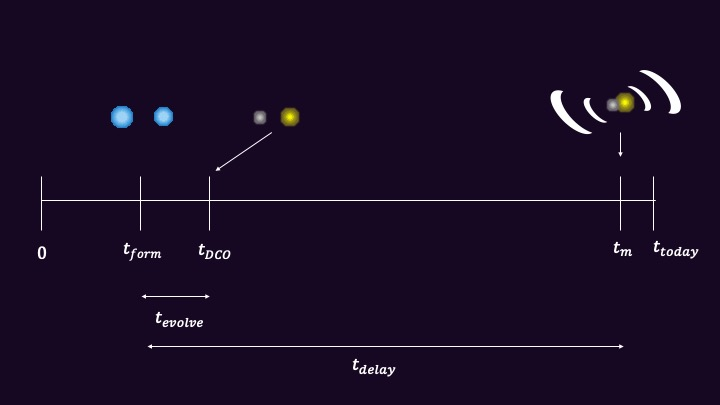
\includegraphics[width=\columnwidth]{../OtherImages/raw_figure_different_timescales.pdf} %angle=90,origin=c
    \caption{Schematic display of the different times in the formation and evolution of a binary system that impact the time \tmerger at which a  \bhnsSingle system will merge in the Universe. The relevant timescales are:  the moment the binary is formed at ZAMS from a gas cloud \tform, the moment of the double compact object (\ac{DCO}) formation \tDCO, the time at which the merger takes place \tmerger, the time it takes the binary to evolve from ZAMS to the \ac{DCO} system $\tevolve = \tDCO - \tform$, the inspiral time \tinspiral and the time between the binary is formed at ZAMS and inspirals $\tdelay = \tmerger - \tform$. We assume in our models that star formation started at redshift $z = 10$.   } 
   \label{fig:timescalesEvolution}
\end{figure}
%


We follow the \ac{PISN} and pulsational-\ac{PISN}  prescription from \citet{2019ApJ...882...36M} as implemented in \citet{2019arXiv190402821S}. 
The mass range of helium cores that undergo \ac{PISN} is shown to be a robust prediction (\citealt{2019ApJ...887...53F}) and we do not expect our particular choice for \ac{PISN} and pulsational-\ac{PISN} prescription to drastically influence our results (see also \citealt{2019arXiv190402821S}).  


The inspiral timescale $\tinspiral$ 
%on which the double compact objects spiral in 
as a result from orbital energy lost in \acp{GW}  is based on \citet{1964PhRv..136.1224P}.


%\begin{enumerate}[label=\arabic*)]
%
%\subsubsection{Stellar winds}
%\label{subsec:bhns-BPS-stellar-winds}
%%
% Line driven stellar winds are an important physical process leading to severe mass loss in  \ac{SN}  progenitors, although the precise mass loss rate and how it evolves in massive stars is uncertain and under debate \citep{2014ARA&A..52..487S,2017A&A...603A.118R}. For  hydrogen rich stars with temperatures $12 500 \leq T \leq 50 000$\Kelvin we implement the line-driven winds from  \citet{2000A&A...362..295V,2001A&A...369..574V} as implemented by \citet[][see their Eqs.~6 and 7]{2010ApJ...714.1217B} which scales with metallicity as\footnote{when taking into account the metallicity dependence of the wind velocity at infinity of $v_{\infty} \propto Z^{0.13}$ from \citet{1992ApJ...401..596L}} $\propto Z^{0.85}$,  which is found to be  in agreement with  observations \citep[][]{2007A&A...473..603M}.  This includes applying an additional luminous blue variable (LBV) wind mass loss of $f_{\rm{LBV}} \cdot  10^{-4}$\Msun\yearmin  independent of metallicity  for stars entering the \citet{1994PASP..106.1025H} limit, see also \citet{2014ApJ...796..121J}. We adopt $f_{\rm{LBV}} = 1.5$ \citep{2010ApJ...714.1217B}.  \floor{to do: add paper Coen? ask Coen/Ilya for other REFs needed)}
%%
%For hydrogen-poor helium stars (which can be observed as Wolf-Rayet stars \citealt{2007ARA&A..45..177C}) we use the winds as applied in  \citet{2010ApJ...715L.138B} which are based on wind rate estimates from  \citet{1998A&A...335.1003H} and the metallicity scaling ($\propto Z^{0.86}$) from \citealt{2005A&A...442..587V}).  In principle, a fraction of the stellar wind could be accreted by its companion, but this is currently not modeled in {\sc{COMPAS}}. 
%%
%	We assume all stellar winds are isotropic and account for the loss in specific angular momentum of the stars. 
%	
%%\floor{ figure out if Im reducing Hamman and Koesterke 98 by a factor of 10 for clumpiness following Yoon et al?}
%, see also appendix B \citet{2019MNRAS.490.3740N} for more details.	

%\subsubsection{Mass transfer stability}
%\label{subsec:method-BPS-mass-transfer-stability}
%%
%When a star expands and exceeds its Roche-lobe radius, mass transfer onto its companion can start. We use the approximation from \citet{1983ApJ...268..368E} for the Roche-lobe radius. The stability of the mass transfer phase is determined based on a comparison of the response of the radius of the donor to (adiabatic) mass loss $\zeta_{*} =  d \log(R_{*}) / d \log(m)$ with the response of the Roche-lobe radius $\zeta_{\rm{RL}} = d \log(R_{\rm{RL}}) / d \log(m)$  to  mass loss during the mass transfer \citep{1972AcA....22...73P,1987ApJ...318..794H,1997A&A...327..620S}.  We assume that if $\zeta_{*}  \geq \zeta_{\rm{RL}}$ that mass transfer is stable. 
%
%We approximate the response of the stars based on their stellar types with $\zeta_{*}  = 2$ for main sequence stars and  $\zeta_{*}  = 6.5 $ for hydrogen shell-burning (i.e. Hertzsprung gap) stars as implemented in \citet[][and references therein]{2018MNRAS.481.4009V} which are based on typical values from \citet{2015ApJ...812...40G}. For stars at later phases we use the fits from \citet{1987ApJ...318..794H,1997A&A...327..620S} for convective stars. 
%
%We assume for our fiducial model that a mass transfer phase from a stripped post-helium-burning star (i.e. case~BB mass transfer \citealt{,1981A&A....96..142D, 1993ARep...37..411T}) onto a \ac{NS} or \ac{BH} is always stable as suggested by  \citet{2015MNRAS.451.2123T,2017ApJ...846..170T}. \citet{2018MNRAS.481.4009V} show that this assumption leads to a better match of population synthesis models to the observed population of  Galactic \ac{NSNS} binaries. 


% Savonije & Takens (1976); De Greve & De Loore (1977)
%\begin{align*}
% d \log(R_{*}) / d \log(m) = 
% \begin{cases} 
% 	2 &\text{for main sequence stars}\\
% 	6.5 &\text{for Herzsprung-gap stars (HG)} \\
% 	
% \end{cases}
%\end{align*}
%based on models from (Ge 2015) Woods


%\subsubsection{Stable mass transfer}
%\label{subsec:method-BPS-stable-mass-transfer}
%%
%We assume that  stable mass transfer occurs on the donor`s thermal timescale and that the companion can 
%accrete until the entire envelope of the donor is accreted  (but see for example \citealt{2017A&A...608A..11G}) at a maximum rate of $\dot{m}_{\rm{acc}} = C \cdot m_{\rm{acc}} / \tau_{\rm{KH}}$, where  $C=10$ following \citet{2002MNRAS.329..897H},  $m_{\rm{acc}}$ is the mass of the accreting star and we approximate the thermal timescale with the  Kelvin-Helmholtz timescale,   $\tau_{\rm{KH}}$, of the donor. 
%
%We assume mass transfer onto a compact object is Eddington-limited. This assumption might not be valid, as suggested from studies including for example \citet[][]{1988ApJ...332..646A,2005ApJ...633..624V,2009MNRAS.397.1836G,2013Natur.493..187M,2014MNRAS.440L..91P,2016MNRAS.461.4496S,2018ApJ...856....6D}. However, van Son et al. (in prep.)  investigate  super-Eddington accretion in {\sc{COMPAS}} and show that this does not drastically change the estimated merger rates for \ac{BHBH} mergers.
%
%%\floor{(See also \citet{2015ApJ...805...20S} for more details.? stability MT)}
%If more mass is transferred from the donor than can be accreted we assume this mass is lost through the vicinity of the accreting star and lost through  `isotropic re-emission'  \citep[e.g.][]{1991PhR...203....1B,1997A&A...327..620S, 2006csxs.book..623T,1975MmSAI..46..217M} and adopt the isotropic loss in specific angular momentum accordingly  \citep[cf. e.g.][]{2008ApJS..174..223B}.  
%
%
%We distinguish between three different cases of mass transfer depending on the stellar phase of the donor star \citep[based on][]{1967ZA.....65..251K,1970A&A.....7..150L}.  Case A is when mass transfer is initiated from a main sequence donor (during core hydrogen burning), case B when mass transfer occurs after the end of core hydrogen burning (i.e. during hydrogen-shell burning or core-helium burning), and case C  when mass transfer is initiated after the end of core helium burning. 
%


%e.g., Soltan 1982; Novak 2013; see also Li 2012  (Page et al. 2013)!! . van Son et al. (2020)  investigate  super-Eddington accretion in {\sc{COMPAS}}.
%
%https://arxiv.org/pdf/1601.05473.pdf: 
%Observationally, evidence for near-Eddington or SE flows has been accumulating in recent years. A study of a large sample of active galactic nuclei (AGNs) suggests that many of them emit considerably more energy and have higher Eddington ratios than previously assumed (Netzer & Trakhtenbrot 2014). Kormendy & Ho (2013) have argued that the normalization of the local \ac{BH} scal- ing relations should be increased by a factor of five to MBH = 0.5% of the bulge mass. This increases the lo- cal mass density in BHs by the same factor, decreases
%the required mean radiative efficiency to 1 - 2%, and may be evidence for radiatively inefficient SE accretion (e.g., Soltan 1982; Novak 2013; see also Li 2012). At high redshifts, the very soft X-ray spectrum of ULAS J1120+0641 appears to suggest that this quasar is ac- creting at super-critical rates (Page et al. 2013). More- over, super-critical accretion onto stellar-mass BHs has been invoked to explain the nature of the ultraluminous X-ray sources (e.g., Gladstone et al. 2009; Middleton et al. 2013).


%and  observations of super massive Quasars in the early Universe \citep{2011Natur.474..616M}.
%showing that super-Eddington accretion is needed to explain the growth of BHs to  
%
%studies that show evidence for super-Eddington accretion rates from both theory  and observations \citep{2018ApJ...856....6D} \citep{2000ApJ...530L..93T}
%



%super-Eddington accretion was originally developed by Abramow- icz et al. (1988) to investigate scenarios where the Eddington lim- itation could be broken. Super-Eddington accretion models of ac- cretion onto stellar mass black holes have recently been investi- gatedbyanumberofauthors(Sa ̧dowski2009;Sa ̧dowskietal. 2014; Sa ̧dowski & Narayan 2016; Sa ̧dowski et al. 2016; Jiang et al. 2017) with results consistently showing that super-Eddington ac- cretion can be achieved with observational evidence also mounting to support super-Eddington accretion (e.g. Du et al. 2018).
%
%and from theory and simulations (e.g. \citealt{1982ApJ...256..681M, 2002MNRAS.335L..13K, 2005ApJ...628..368O,2007MNRAS.377.1187P, 2012MNRAS.425.2892W, 2015MNRAS.447L..60S,2015ApJ...804..148V,2016MNRAS.459..171S}).  
%
%, e.g.   ultra-luminous X-ray sources  \citep{2014Natur.514..202B, 2017Sci...355..817I,2017Sci...355..817I,2017MNRAS.466L..48I,2001ApJ...552L.109K, 2001ApJ...549L..77W}, narrow-line Seyfert-1 galaxies \citep{2000PASJ...52..499M, 2017MNRAS.471..706J}   , quasars \citep{2002A&A...388..771C,2012MNRAS.427.1867A} and the  rapid growth of super-massive BHs   \citep{1999MNRAS.308..302Z}  (Volonteri et al. 2015; Begelman $\&$ Volonteri 2017) 
%


% see https://arxiv.org/pdf/1703.10728.pdf, https://authors.library.caltech.edu/96477/1/1903.06844.pdf and https://arxiv.org/pdf/1709.02845.pdf

%see also the system SS433 \citep{2004ASPRv..12....1F},  
%(but see e.g. van Son et al. 2020 for a study where this assumption is investigated)
%
%\subsubsection{Common-envelope phase}	
%\label{subsec:method-BPS-common-envelope}
%%	
% Unstable mass transfer in a binary can lead to a common-envelope (CE) phase during which the two stars are engulfed in the shared envelope and drastically decrease their separation \citep{1976IAUS...73...75P,2001ASPC..229..239P}. CEs are thought to be especially relevant for the formation of  double compact objects in tight orbits \citep{1976IAUS...73...35V,2013A&ARv..21...59I}  \floor{add pop synth CEE studies like Dominik et al. 2012, Belczynski,2002,2018? (Alejandro says: maybe not, otherwise you need to cite 100s papers...)}.  
%We follow the simplified $\alpha$-$\lambda$ prescription from \citet{1984ApJ...277..355W,1990ApJ...358..189D} to parameterize the \ac{CE} phase. 
%We assume for the $\alpha$ parameter the value $\alpha=1$ in our fiducial model but vary this to $\alpha = 0.1$ and $\alpha=10$ (see Table~\ref{tab:variations-BPS}). For the $\lambda$ parameter we use the fitting formulas from \citet{2010ApJ...716..114X,2010ApJ...722.1985X}, which is similar to the $\lambda_{\rm{Nanjing}}$ parameter in \citet{Dominik:2012kk}. In this method the value of $\lambda$  depends on the stellar evolutionary stages of the stars (see also \citealt{2000A&A...360.1043D,2001ASPC..229..255D,2001A&A...369..170T,2016A&A...596A..58K}). 
%
%%(see e.g. Dewi & Tauris 2000, 2001; Kruckow et al. 2016).
%We assume that successful \ac{CE} ejections  lead to circularization of the orbit \citep{2013A&ARv..21...59I}. 
%%%
%%where the final separation is calculated by using
%%\begin{align}
%%\frac{a}{a_0} = 	\frac{m_{2,\rm{core}}}{m_2} \left(  1 + \frac{2}{\alpha \lambda} \frac{m_{2, \rm{env}}}{m_1}  \frac{a_0}{R} \right)^{-1}
%%\end{align}	
%%
% We also assume that a stellar merger occurs when one of the stars in a binary system fills its Roche-lobe immediately after the ejection of the \ac{CE} (and the \ac{CE} thus `failed'). 
% 
%We don't allow donor stars which are hydrogen shell burning (i.e. Hertzsprung gap stars) and engage in a \ac{CE} event to survive in our fiducial model. These donor stars are not expected to have developed a steep density gradient between core and envelope  \citep{2000ARA&A..38..113T,2004ApJ...601.1058I}  making it challenging to successfully eject the envelope. Instead, a merger takes place.  This implementation follows the `pessimistic' \ac{CE} scenario from \citet{Dominik:2012kk}.  The `optimistic' \ac{CE} scenario, on the other hand, assumes these systems can survive.    Which of the scenarios more accurately represents observations is still under debate.   Recently, \citet{2017MNRAS.472.2422M} show that the pessimistic scenario slightly better matches the predicted  \ac{BHBH}  rate.   \citet{2018MNRAS.481.4009V}  argue that there is no clear evidence to favor one of the scenarios over the other based on a study of Galactic \ac{NSNS}  binaries.  
%We decide to use the pessimistic model as fiducial assumption, similar to recent  population synthesis studies including \citet{2018MNRAS.480.2011G,2019ApJ...885....1W,2019MNRAS.490.3740N} and use the optimistic assumption as a model variation (see Table~\ref{tab:variations-BPS}). % and Belczynski, \href{arXiv:1806.00001v1}{Mapelli}
%	More details and discussion of the treatment of CEs in {\sc{COMPAS}} are discussed in \citep{2020arXiv200109829V}. 

	
%\todo{To do: check whether I also allow MS in CEE (like CEE paper Alejandro.. I dont think so) see hidden comment:} %Check if you have this in your pythonSubmit:
%    common_envelope_allow_main_sequence_survive = True      # Allow main sequence stars to survive CE. Was previously False by default 
%\floor{add If one of the stars in the post-CE binary is filling its Roche lobe immediately after \ac{CE} ejection, we assume that there is insufficient orbital energy available to eject the envelope and the binary evolution is terminated in a merger.}
%%



%\subsubsection{Core-collapse \ac{SN}  prescription}
%\label{subsec:method-BPS-ccSN}
%%
%%(Belczynski et al. 2012) This mass gap could be indicative of the \ac{SN}  explosion mechanism (Belczynski et al. 2012).
%We use the \textit{delayed} \ac{SN}  remnant mass prescription \citep{2012ApJ...749...91F}  to map the carbon-oxygen core masses of stars to compact object remnant masses during core-collapse \ac{SN}  events. We deviate with this choice from most binary population synthesis codes that typically  use instead the \textit{rapid} \ac{SN}  remnant mass prescription for their fiducial model (examples include \citealt[][]{2018arXiv181200012K, 2019arXiv191100903B},  but see e.g. also the discussion in \citealt{2019arXiv191203599E} on why this assumption may need to be revisited). The {rapid} prescription assumes \ac{SN}  explosions occur within 250 ms (compared to longer timescales assumed for the delayed prescription) and reproduces, by construction,  the  lower remnant mass gap between NSs and BHs that is apparent from  X-ray binary observations 
%\citep{1998ApJ...499..367B, 2010ApJ...725.1918O, 2011APS..APRH11002F} by a lack of BHs in the mass range between about the heaviest neutron stars  $\sim$ 2--3\Msun \citep{2016ARA&A..54..401O, 2017ApJ...850L..19M, 2019NatAs.tmp..439C,2019arXiv190801012T,2020arXiv200106102S} and  BHs of $\sim$ 4--7\Msun. \question{Should I discuss that  merging \ac{NS} product can fall in \ac{BH} gap?} % \citep{2015ApJ...801...90P,2019ApJ...882L..24A}. 
%% 


%	It is still under debate whether this lower \ac{BH} mass gap exists. Theoretical models of supernovae both predict a gap \citep{2014ApJ...785...28K,2015ApJ...801...90P} and a smoother (e.g. \citealt{1995ApJS..101..181W,2001ApJ...554..548F,2019arXiv191001641E})  distribution between \ac{NS} and \ac{BH} remnant masses. But see also \citet{2020MNRAS.491.2715B} who point out that it is very challenging to model remnant masses from supernovae explosions and that the compactness measure that is often used in these \ac{SN}  remnant mass studies is not a good metric for explodability of the supernova. 
%	Moreover, \citet{2012ApJ...757...36K}   show evidence that the apparent observed mass gap from BHs in X-ray binaries could be caused by systematic offsets in the \ac{BH} mass measurements.  
%	More recently, \citet{2019Sci...366..637T} found evidence for a $3.3_{-0.7}^{+2.8}$\Msun mass \ac{BH} observed in a non-interacting binary with a red giant, which is in addition of earlier observation of a speculated $\sim 2.44\pm0.27$\Msun \ac{BH} \citep{2002A&A...392..909C,2010AAS...21541905R,2011arXiv1107.1537D}. 
%	In addition,  \citet{2016MNRAS.458.3012W,2019arXiv190407789W} studied microlensing events of BHs based on  observations from OGLE-III and Gaia data release 2.  
%	They find evidence for a continuous distribution of stellar remnant masses and disfavor a mass gap between NSs and BHs (unless BHs receive natal-kicks above 20-80\kms).   
%	In addition, the LIGO-Virgo Collaboration reported at the time of writing three candidate \ac{GW} events in their O3 observation run with at least one component in the lower mass gap \citep{GCNS190924h,GCNS190930s,GCNSS200115j}.	
%%	We therefore conclude that based on the above, there is no clear evidence that the rapid remnant mass prescription  should be preferred in population synthesis simulations. 
%	
%Moreover, \citet{2018MNRAS.481.4009V} show that the delayed prescription better matches the observed distribution of masses of Galactic double \ac{NS} systems. 
%We  therefore adopt the delayed remnant mass prescription and vary this to the rapid prescriptions as one of our model variations (see Table~\ref{tab:variations-BPS}). \\
%	

%
% We fixed a small bug in the implementation of the delayed remnant mass prescription from  \citet{2012ApJ...749...91F} in  {\sc{COMPAS}}. 
% This bug  lead in previous simulations with the {\sc{COMPAS}} code incorrectly to an additional gap in the neutron star remnant mass distribution around  2.2\Msun. See Appendix~\ref{sec:app-Fryer-bug-fix} for more details. 
%
% 
% \floor{discuss with Edo:  \ac{SN} metallicity dependency; not in remnant function but in ZAMS to CO mapping}

%
%\subsubsection{Ultra-stripped supernova}
%\label{subsec:method-BPS-USSN}
%%
%Case BB mass transfer from a companion star onto a \ac{NS} or \ac{BH} in short period binaries leads to \floor{severe} stripping (i.e. leaving behind an envelope with mass $\lessapprox 0.1$\Msun) by the compact object and we assume the stripped star eventually undergoes an ultra-stripped \ac{SN}  (USSN) as shown by \citet{2013ApJ...778L..23T,2015MNRAS.451.2123T, 2015MNRAS.454.3073S, 2017MNRAS.466.2085M,2018MNRAS.479.3675M}. We follow with this the prescription of the fiducial model of \citet{2018MNRAS.481.4009V}, but we deviate by also assuming case BB mass transfer onto a \ac{BH}  leading to an ultra-stripped \ac{SN}  as suggested by \citet{2013ApJ...778L..23T,2015MNRAS.451.2123T}  and in agreement with the implementation of ultra-stripped \ac{SN}  in e.g.  \citet[][]{2018MNRAS.481.1908K, 2019arXiv191100903B}.   We calculate the remnant mass of an ultra-stripped \ac{SN}  using the \textit{delayed} Fryer prescription \citep{2012ApJ...749...91F}. 
%% \floor{make into 2 seperate points? USSN and case BB?}
%. Preliminary results with David Aguilera-Dena show they do, but think it has not been explicitly proved in the literature.
%\floor{check work by David Aguilera-Dena by time of publication (currently not out yet)}

%\subsubsection{Electron-capture \ac{SN}  }
%\label{subsec:method-BPS-ECSN}
%%
%We assume stars on the asymptotic branch with helium core masses between 1.6--2.25\Msun \citep{2002MNRAS.329..897H}  lead to electron-capture \ac{SN}  (ECSN) \citep{1980PASJ...32..303M, 1984ApJ...277..791N,1987ApJ...322..206N, 2008MNRAS.386..553I}, (lower  core masses will lead to the formation of white dwarfs). 
%	
%	If a star undergoes an electron-capture \ac{SN}  we set its remnant mass to 1.26\Msun, as an approximation to the solution of Equation~8 in \citet{1996ApJ...457..834T}. %$m_{\rm{baryonic}} - m_{\rm{grav}} = 0.075 m^2_{\rm{grav}}$ to the solution of the quadratic formula for the baryonic and gravitational remnant masses   from 
	
%	
%	 with degenerate oxygen-neon-magnesium cores above 1.38\Msun never develop an iron core and collapse due to electron captures onto the Magnesium and Neon leading to sudden drop in the electron-pressure support in the core and the rise of an electron-capture \ac{SN}  (Miyaji et al. 1980; Nomoto 1984,Nomoto 1987, 1987; Ivanova et al. 2008). In COMPAS we assume helium core masses between 1.6--2.25\Msun lead to electron-capture \ac{SN}  based on \citet{2002MNRAS.329..897H}. More recently, \citet{2004ApJ...612.1044P} argued  other ranges are more realistic and (\citealt{2015ApJ...801...32A}, Vinciguerra. in prep.) showed a different range could better reproduce observations of neutron stars. However, these conlusions haven't converged. 
	
	
%	We assume the baryonic mass of the degenerate ONeMg core leading to an ECSN is 1.38 M? (Nomoto 1987). We approximate the ECSN rem- nant mass as mECSN = 1.26 M? using the quadratic approx- imation mbar −mgrav = 0.075m2
%grav (Timmes et al. 1996)
%	%
%	%%%%%%%%%%%%%%%%%%%%%%%%%%%%%%%%%%%%%

	
%	
%	%%%%%%%%%%%%%%%%%%%
%\subsubsection{\ac{SN}  natal kicks and fallback}
%\label{subsec:method-BPS-SN-natal-kick-and-fallback}
%NSs and BHs receive \ac{SN}  kicks at birth.  
%	For core-collapse \ac{SN}  these natal kick magnitudes are drawn from a Maxwellian velocity distribution with a one-dimensional root-mean-square velocity dispersion of $\sigma = 265$\kms, based on observations of radio pulsar proper motions  \citep{2005MNRAS.360..974H}.
%	
%	For ultra-stripped and electron-capture \ac{SN}  we use instead  a  one-dimensional root-mean-square velocity dispersion of  $\sigma = 30$\kms  following \citet{2002ApJ...571L..37P,2004ApJ...612.1044P}, which is in agreement with the subset of double \ac{NS} and pulsars observed with low  velocities and small eccentricities  \citep{2010ApJ...719..722S,2016MNRAS.456.4089B, 2002ApJ...571..906B,2017ApJ...846..170T, 2017A&A...608A..57V, 2017JApA...38...40V}. 
%Combined, the magnitude of  \ac{SN}  kicks is thus drawn from a bi-modal distribution as suggested by \citet{1975Natur.253..698K,2002ApJ...568..289A}.
%		All natal kicks from supernovae are assumed to be isotropic  and we sample the kick polar angles $\theta_k$ and kick azimuthal angles $\phi_k$ from a unit sphere.  
%	 During the \ac{SN}  event a fraction of the ejected material, $f_{\rm{fb}}$, is assumed to fallback onto the compact object. We use the prescription from Eqs.~16 and 19 in  \citet{2012ApJ...749...91F} to determine this fraction and reduce the natal kick by a factor ($1-f_{\rm{fb}}$) accordingly. This typically reduces the natal kicks of BHs with carbon-oxygen cores above 11\Msun  (for the delayed \ac{SN}  prescription) to zero. This is in agreement with observations  that show evidence that  BHs might form with lower or no natal kicks although this is still under debate  \citep[][]{1999A&A...352L..87N,2012MNRAS.425.2799R,2013MNRAS.434.1355J,2015MNRAS.453.3341R,2016MNRAS.456..578M}. %,  see also \citealt{2013MNRAS.434.1355J}  and references therein. 
%	 %
%	 For ultra-stripped and electron-capture \ac{SN}  we use instead  a  one-dimensional root-mean-square velocity dispersion of  $\sigma = 30$ \kms  which is in agreement with the subset of double \ac{NS} / Pulsar systems observed with low velocities and small eccentricities \citep{2017ApJ...846..170T} (Tauris et al. 2017).  
	%bimodal  \ac{SN} distribution (e.g., Katz 1975; Arzoumanian et al. 2002).
	
%	All natal kicks from supernovae are assumed to be isotropic  and we sample the kick polar angles $\theta_k$ and kick azimuthal angles $\phi_k$ from a unit sphere. 
	
%	We reduce our parameter space by not drawing mean anomalies of the orbit at the moment of the supernova, as we assume the binary to be circular at the moment of the supernova. \floor{Should I add a reference of similar codes that do this (basically all)?}
	
%	don't draw a mean anomalies of the orbit are assum at the moment of the \ac{SN}  event from the range $[0,2\pi]$. \floor{(give ref? I could say: see e.g. dart board??)} \floor{double check the parameter ranges, is this right?}.

%\subsubsection{Pair-instability supernovae}
%\label{subsec:method-BPS-PISN}
%%
% The existence of a \ac{BH} mass gap of an absence of BHs with masses in the range $\sim 50$--$150$\Msun is suggested from both observations \citep{2017ApJ...851L..25F,2018ApJ...856..173T,2019PhRvX...9c1040A, 2019PhRvD.100d3012W, 2019MNRAS.484.4216R,2019arXiv191209708G} and theory \citep{1964ApJS....9..201F,1967PhRvL..18..379B,2017ApJ...836..244W}. Stars with helium cores in these mass ranges are thought to become unstable to electron positron pair production, eventually leading to a pair-instability \ac{SN}  (PISN) explosion that leaves behind no remnant  \citep{1964ApJS....9..201F,1967PhRvL..18..379B,1968Ap&SS...2...96F,2019ApJ...887...72L,2019ApJ...878...49W}.  In addition, there is also evidence from theory that stars with helium core masses in the range $\sim 30$--$60$ lead to pulsational-PISN \citep[e.g.][]{2017ApJ...836..244W,2016MNRAS.457..351Y,2017MNRAS.470.4739S,2019ApJ...882...36M, 2020arXiv200205077R}, where in several pulses material is ejected but a \ac{BH} still forms. These pulsations remove the hydrogen envelope of the star and cause the stars to form BHs with masses in a narrow range resulting to an excess of BHs around the range $\sim$35--45\Msun  which has also been suggested from observations \citep{,2018ApJ...856..173T,2019PhRvX...9c1040A}. 
%% leading to an excess of BHs in the range $\sim 30$--$45$\Msun \citep{,2018ApJ...856..173T}.  
%
%We follow the PISN and pulsational-PISN  prescription from \citet{2019ApJ...882...36M} as implemented in \citet{2019arXiv190402821S}. The location of the PISN is shown to be a robust prediction (\citealt{2019ApJ...887...53F}) and we don't expect our particular choice for PISN and pulsational-PISN prescription to drastically influence our results (see also \citealt{2019arXiv190402821S}).  

%\floor{add Mathieus paper when its out.}
%	\floor{should I say something about the metallicity at which this occurs or go in more depth to what `implementing marchant2018' means?} 
	
%	\floor{(mention results from \citet{2017MNRAS.470.4739S}?? )}
	
%\citep[e.g.][]{2014A&A...566A.146K, 2017MNRAS.464.2854K}
%\floor{finish Mathieu's comments:}
%\floor{ot sure that Kozyreva's citations are properly placed for this statement (she does spectral synthesis of the explosions, not work on the remnant), barkat+67 is more appropriate. Also, no need to cite Fowler & Hoyle 64 twice, once is enough, and maybe instead cite Leung+19 and Woosley 19. Finally, maybe you should spend an extra word explaining why the excess of \ac{BH} in the range 30-45Msun and you are missing citations to Spera, Mapelli et al. that implemented PPISN recipes based on Woosley's work in SEVN that are relevant.
%}	
	
	%2014A&A...565A..70K
	
	
%in the frame of reference of the exploding star and ran- domly drawn from a unit sphere. For the magnitude of the natal kicks of the SNe, we assume a bimodal distribu- tion (e.g., Katz 1975; Arzoumanian et al. 2002). For CCSN, we draw natal kick magnitudes from a Maxwellian velocity distribution with a one-dimensional standard deviation of σhigh = 265 km s−1 following the 3D pulsar velocity distri- bution derived by Hobbs et al. (2005) from a subset of their 2D observations. USSN and ECSN natal kick magnitudes are drawn from a Maxwellian velocity distribution with a one- dimensional standard deviation of σlow = 30 km s−1, follow- ing Pfahl et al. (2002a) and Podsiadlowski et al. (2004). This second component is introduced to match the observed low natal kicks in some Galactic DNSs (Schwab et al. 2010; Be- niamini & Piran 2016) as well as in isolated pulsars (Brisken et al. 2002), as the single-mode isolated pulsar velocity dis- tribution proposed by Hobbs et al. (2005) fails to predict the low-velocity pulsar population as discussed by Verbunt et	
	
	

%	
%
%\subsubsection{\ac{GW} inspiral time}	
%\label{subsec:method-BPS-GW-inspiral-time}
%%
%
%We determine the coalescence timescale on which the double compact objects spiral in as a result from orbital energy lost in \acp{GW}  by  \citep{1964PhRv..136.1224P}
%\begin{equation}
%	\tinspiral = \frac{15}{304} \frac{a_0^4 c^5}{G^3 m_1 m_2 (m_1 + m_2)} \tau(e_0),
%\end{equation}
%%% \cdot	 \left[  (1-e_0^2) e_0^{- \frac{12}{19}} \left( 1+\frac{121}{304}e_0^2  \right)^{-\frac{870}{2299}}  \right]^4
%where $a_0$ and $e_0$ are the separation and eccentricity of the binary after the second supernova, $c$ is the speed of light in vacuum,  $G$ is the Newtonian gravitational constant, $m_1$, $m_2$ are the two component masses of the binary and $\tau(e_0)$ is a function of the eccentricity given by
%
%\begin{align*}
%\begin{split}
%	\tau(e_0) = 	 \left[  (1-e_0^2) e_0^{- \frac{12}{19}} \left( 1+\frac{121}{304}e_0^2  \right)^{-\frac{870}{2299}}  \right]^4\\ 
%	 \cdot \int_0^{e_0} \frac{e^{29/19} (1+\frac{121}{304}e^2)^{\frac{1181}{2299}}}{(1-e^2)^{\frac{3}{2}}} \, \rm{d}e. 
%\end{split}
%\end{align*}
%%





%\floor{this might be important as many massive stars experience rapid rotation during their evolution (see \href{https://arxiv.org/pdf/1211.3742.pdf}{de Mink 2012 } and references therein)}

\subsubsection{The formation, evolution, inspiral and delay times}	
\label{subsec:method-BPS-different-timescales-binary}
%
%To calculate  \bhnsSingle merger rates, it is important to consider the different timescales that combined determine the time at which a system merges in our Universe. 
The time at which a \ac{DCO} merges, \tmerger,  is given by the sum $\tmerger = \tform + \tevolve + \tinspiral$, shown in Figure~\ref{fig:timescalesEvolution}, with $\tform$ the time at which the initial binary forms from a gas cloud since the   the beginning of star formation in the Universe, \tevolve the time it takes the binary from birth at the ZAMS to form a double compact object (i.e. until the second SN) and \tinspiral the time  it takes the double compact object to coalescence from the moment of the second SN. 
%These timzxes are schematically depicted in Figure~\ref{fig:timescalesEvolution}. 
The formation and inspiral time together form the delay time $\tdelay = \tevolve+ \tinspiral$, such that  
%
\begin{align}
\tform = \tmerger - \tdelay. 
\label{eq:delay-time}
\end{align}
%
%The different timescales are also depicted in .

\subsubsection{Initializing a population of \bhnsSingle mergers}
\label{subsec:selecting-a-population-of-BHNS-mergers}
%
%
For each binary population synthesis model  we evolve a population of about  $10^6$ binary systems per metallicity $\Zi$ from birth until they form a double compact object binary or otherwise merge or disrupt. From the population of \ac{DCO} binaries we select the \bhnsSingle systems. We also select only the binaries that merge in a Hubble time, (i.e. that have \tdelay $\leq t_{\mathcal{H}}$) with $t_{\mathcal{H}} =  \mathcal{H}_0^{-1} = 13..77$\,Gyr \citep{2016A&A...594A..13P}  for the WMAP9--cosmology \citep{2013ApJS..208...19H}\footnote{obtained from the astropy cosmology module, which has  $\Omega_{\rm{m}}=0.308, \Omega_{\Lambda}^0= 0.7185, \Omega^0_{\rm{b}}=0.04628$.} . 

We use {\COMPAS} to calculate and record properties such as the ages, masses, stellar radii, effective temperatures, velocities, eccentricities,  and separations of the binary at important evolutionary stages of the binary such as mass transfer episodes and supernovae. \COMPAS also records \tevolve and \tinspiral for each \bhnsSingle system. 


%Can you try to set the accretion efficiency to 0.5 and the specific  angular momentum = 1 (for the SMC metallicity I can if you want have a double check before if it makes any difference in the q distributions)



Throughout the rest of the paper we will use the notation \bhnsSingle for binaries containing a \ac{BH} and a NS. The notation BH--NS  (NS--BH) will be used when we explicitly refer to a \bhnsSingle binary where the \ac{BH} (NS) formed in the first supernova. The formation order is known in stellar evolution simulations but  not known in (gravitational-wave) observations.  The formation order is particularly important for spinning up the \ac{BH} or \ac{NS} and the formation of millisecond pulsars. 




\subsection{Calculating the \bhnsSingle formation rate per $M_{\rm{SFR}}$}
\label{subsec:method-BPS-merger-rate-per-M-SFR}
%


Using the selections in Section~\ref{subsec:selecting-a-population-of-BHNS-mergers} we obtain at the end of a simulation  a  population of  \bhnsSingle systems that merge in a Hubble time  simulated over 30 different metallicities.  However, the efficiency of \bhnsSingle merger formation is much higher in our simulations compared to their occurrence rate in the Universe because we model only a small fraction of the underlying stellar population   by, neglecting single stars, not simulating binaries with primary star masses below $5$\Msun and not drawing binaries from their initial birth distributions.

To calculate the \bhnsSingle formation rate, we therefore re-normalize the population synthesis model to obtain a formation rate of \bhnsSingle mergers for a given metallicity $\Zi$ per unit star forming mass, i.e. $\diff \Nform / \diff \MSFR$, and calculate the formation rate for \bhnsSingle mergers with a given delay time and final compact object masses in {\sc{COMPAS}} with
%
\begin{align}
%
&\rate_{\rm{form}}(\Zi, \tdelay, \monef, \mtwof) = \notag \\
& \frac{\diff^4 \Nform}{\diff \MSFR \diff \tdelay \diff \monef \diff \mtwof} (\Zi, \tdelay, \monef, \mtwof).
%
\label{eq:formation-rate-COMPAS}
\end{align}
%

We calculate this re-normalized formation rate by incorporating the {\sc{STROOPWAFEL}} weights and assuming a fixed binary fraction of $f_{\rm{bin}} = 0.6$, which  is  consistent with the observed intrinsic binary fraction for O-stars  \citep{2011IAUS..272..474S, 2015A&A...580A..93D, 2017A&A...598A..84A, 2017IAUS..329..110S}. This choice for the binary fraction is slightly lower than the 0.7 from \citet{2012Sci...337..444S} or the $f_{\rm{bin}}=1$ that is often assumed in binary population synthesis simulations.
% but likely better reflects effects from triples and metallicity dependence \floor{REF (Ilya/Stephen/Selma?)}. 
More details on the re-normalization of the \bhnsSingle formation rate can be found in  \CMP.


\subsection{Calculating the cosmological \bhnsSingle merger rate}
\label{subsec:method-MSSFR}
\bhnsSingle systems form from their initial stars in several million years, but their inspiral times typically span many Gyrs \citep{1994MNRAS.268..871T, 1998A&A...332..173P, 1999ApJ...526..152F, 2002ApJ...572..407B, 2016A&A...589A..64M,Mapelli:2017hqk}. 
%
The \acp{GW}  therefore typically originate from binaries formed at high redshifts and  from stars with low initial metallicities  \citep[see e.g.][]{2018MNRAS.480.2704L}.  
% Both the amount of star formation and the metallicity of the star forming gas is strongly dependent on redshift \todo{(add REF)}. 
% And since the stellar evolution outcome depends strongly on the metallicity of the stars, this results in the  \bhnsSingle merger rate being strongly impacted by the unknown metallicity-specific star formation history of our Universe. 
% We therefore 
% Both uncertainties can lead to order of magnitude uncertainties in the merger rates of double compact objects \citep{2019MNRAS.488.5300C, 2019MNRAS.490.3740N} 
%
The rate of \bhnsSingle mergers strongly depends on the star formation rate (SFR) and the metallicity of the stars, which both depend on the redshift at which the initial binary system is formed at ZAMS.  
%This is because at higher SFRs,  more binaries are formed and hence also more \bhnsSingle mergers form. 
The evolution of stars is strongly impacted by metallicity, which impacts mass loss through stellar winds,  the stellar radii (and radial expansion)  and  thereby the outcome of the evolution \citep[e.g.][]{1992A&A...264..105M}. The metallicity therefore strongly  impacts the rate of double compact object mergers and their characteristics such as final masses  \citep[see e.g.][]{2016MNRAS.462.3302E,2019MNRAS.482.5012C}.


%The \bhnsSingle merger rate is thus a function of the 
To calculate the \bhnsSingle merger rate  that can be observed with \acp{GW} today, we therefore first integrate the formation rate from Equation~\ref{eq:formation-rate-COMPAS} over  metallicities and use  the relation $\tform = \tmerger - \tdelay$ to obtain the merger rate for a binary with masses \monef, \mtwof at any given merger time \tmerger with

%The \acp{GW} that we observe today could therefore origin from binaries formed at high redshifts and  from stars with metallicities much lower than solar-metallicity \citep[see e.g.][]{2018MNRAS.480.2704L}.  Both the amount of star formation and the metallicity of the star forming gas is strongly dependent on redshift \todo{(add REF)}. And since the stellar evolution outcome depends strongly on the metallicity of the stars, this results in the  \bhnsSingle merger rate being strongly impacted by the unknown metallicity-specific star formation history of our Universe. Both uncertainties can lead to order of magnitude uncertainties in the merger rates of double compact objects \citep{2019MNRAS.488.5300C, 2019MNRAS.490.3740N} \floor{add pop synth REF for first unc.}. 
%
\begin{align}
%
&\rate_{\rm{m}} (\tmerger) = \frac{\diff^4 \Nmerger }{\diff \ts \diff \Vc  \diff \monef \diff \mtwof} (\tmerger)  \notag \\
%
		&= \int \diff Z  \int_0^{\tmerger} \diff \tdelay \, { \rm{MSSFR}}(\tform) \, \times \notag \\ 
		&\, \hspace{3cm} \rate_{\rm{form}}(Z, \tdelay, \monef, \mtwof),  
%
\label{eq:MSSFR-merger-rate}
\end{align}
%
where \ts is the time in the source frame of the merger, \Vc is the comoving volume, $\rate_{\rm{form}}$ is obtained using {\sc{COMPAS}} (see Section \ref{subsec:method-BPS-merger-rate-per-M-SFR}) and ${\rm{MSSFR}}(\tform)$ %
is the metallicity-specific \ac{SFR}  at formation time \tform. We obtain the \ac{MSSFR} by 
multiplying a \ac{SFR}   with a metallicity density function
%
\begin{align}
%
	&{\rm{MSSFR}}(z_{\rm{form}}) = 
	\frac{d^3 \MSFR}{d \ts d \Vc dZ}(z_{\rm{form}})  
	 \notag \\
	 &= \underbrace{\frac{d^2 \MSFR}{d \ts d \Vc }(z_{\rm{form}})}_\text{SFR} 
	 \times 
	 \underbrace{\frac{d \MSFR }{dZ}(z_{\rm{form}})}_\text{GSMF $+$ MZR}, 
	 \label{eq:MSSFR-equation}
\end{align}
%
where we wrote down the equations in redshift $z$ and used the short hand notation $z_{\rm{form}} = z(\tform)$.  We use for the metallicity density function a convolution between a \ac{GSMF} and  \ac{MZR} which are discussed below.



This  merger rate $\rate_{\rm{m}}$ is then converted to a local detection rate by  integrating over the co-moving volume and taking into account the probability \Pdet  of detecting a  \ac{GW} source (see Section~\ref{subsec:detection-probability}) with 


%
\begin{align}
\label{eq:rate_detector}
%
	&\rate_{\rm{det}}(\tdet, \monef, \mtwof) = 
	\frac{\diff^3 \Ndet}{\diff \tdet  \diff \monef \diff \mtwof} 
	\notag  \\
%
	&= \int 
	\diff \Vc  \,
	 \frac{\diff \ts}{\diff \tdet}  \,  
	 \rate_{\rm{m}}(\tmerger) \, 
	  \Pdet (\monef, \mtwof, \DL(z)),
%
\end{align}
%
where \tdet is the time in the detector (i.e. the observer) frame. 


In practice, the integral in Equation~\ref{eq:rate_detector} is estimated using  Monte Carlo estimates over redshift, metallicities and delay time bins. This method is similar to previous work by e.g.,   \citet{2013ApJ...779...72D, 2015ApJ...806..263D,2016ApJ...819..108B,2016MNRAS.458.2634M, 2018MNRAS.477.4685B, 2019MNRAS.482..870E, 2019PhRvD.100f4060B,2019arXiv190612257B, 2019MNRAS.482.5012C}. Our cosmological merger rate calculation follows closely the method of \citet{2019MNRAS.490.3740N}. Details of the method and  the derivation of the cosmological merger rate equations are given in \citet{2019MNRAS.490.3740N} and \CMP.


% 
\begin{table*}
%
\label{tab:MSSFR-variations}
\resizebox{\textwidth}{!}{%
\centering
\begin{tabular}{llll}
\hline
\hline
{xyz} index &  \ac{SFR}                     & \ac{GSMF}       & \ac{MZR}                        \\ \hline \hline
0 (fiducial)   				& \multicolumn{3}{c}{ phenomenological     \citet{2019MNRAS.490.3740N} }          \\
\hline
%
1              			       	& {\citet{2014ARA&A..52..415M}}  &  \citet{2004MNRAS.355..764P} & \citet{2006ApJ...638L..63L}   \\
%
2              					&  \citet{2004ApJ...613..200S}							& \citet{2015MNRAS.450.4486F} single Schechter   & \citet{2006ApJ...638L..63L} $+$ offset    \\
%
3              			      	& \citet{2017ApJ...840...39M}     		& \citet{2015MNRAS.450.4486F} double Schechter          &  \citet{2016MNRAS.456.2140M}             \\ \hline
\end{tabular}%
}
%
\caption{List of the assumptions for the metallicity-specifc star formation rate (MSSFR) models  that we explore in this study. All \NmodelsMSSFR \ac{MSSFR} models are obtained by combining a star formation rate (SFR) with a galaxy stellar mass function (GSMF) and mass-metallicity relation (MZR). See  Sections~\ref{subsec:method-MSSFR} and \ref{subsec:MSSFR-variations} for more details. The models are named in the convention $\mu\rm{xyz}$ with respectively $\rm{x, y, z} \in [1,2,3]$ the index numbers for the models used for the  \ac{SFR} , \ac{GSMF} and \ac{MZR} respectively.  For example, the combination of using the {\citet{2014ARA&A..52..415M}} \ac{SFR}  with the  \citet{2004MNRAS.355..764P} \ac{GSMF} and \citet{2016MNRAS.456.2140M}  \ac{MZR}  is labeled $\mu{113}$. The fiducial (phenomenological) model is not a specific combination but a parameterized model that is build to be flexible and is fitted to match the observed \ac{BHBH} rate and chirp mass distribution from the first two runs of LIGO and Virgo \citet{2019MNRAS.490.3740N}. The phenomenological  model has the label $\mu{000}$ }
%
\label{tab-MSSFR-variations-labels}
\end{table*}




\subsection{MSSFR prescriptions}
\label{subsec:MSSFR-variations}
%
We use combinations of assumptions for the \ac{SFR} , \ac{GSMF} and \ac{MZR} prescriptions that together make up the \ac{MSSFR} model in Equation~\ref{eq:MSSFR-equation}. These models are  summarized in Table~\ref{tab:MSSFR-variations} and described in \citet{2019MNRAS.490.3740N} and references therein. In total this results in \NmodelsMSSFR \ac{MSSFR}  variations: 27 from the combinations of \ac{SFR},  \ac{GSMF} and \ac{MZR}  and one from  the phenomenological model from  \citet{2019MNRAS.490.3740N}  that we use as  fiducial model. 


In Section~\ref{sec:results-variations} we show that the shape of the predicted \bhnsSingle distributions is relatively robust under these \ac{MSSFR} variations. We highlight in most figures the following three \ac{MSSFR} variations:

$\mathit{{\mu000}}$ --  This is our fiducial model which is the  phenomenological model from \citet{2019MNRAS.490.3740N}. This  model uses parameterized  equations for the \ac{SFR}  and the metallicity distribution, where the values of those free parameters  are found by combining the parameterized  \ac{MSSFR} prescriptions with a population synthesis outcome to find the  best fit to the \ac{GW} observations announced in the first two observing runs of LIGO and Virgo   \citep{2019MNRAS.490.3740N}. This work is also done with  {\sc{COMPAS}} using stellar-evolution assumptions that are similar to the ones assumed in this study, and we therefore expect the merger rates based on this \ac{MSSFR} choice and our fiducial simulations to be representative for the \ac{GW} observations from \acp{BHBH}. 

The  \ac{SFR}  that is found in the phenomenological model of \citet{2019MNRAS.490.3740N} follows the \ac{SFR}  shape of  \citet{2014ARA&A..52..415M, 2017ApJ...840...39M} but has a slightly higher \ac{SFR}  at higher redshifts. It also has a smaller \ac{SFR}  compared to \citet{2004ApJ...613..200S} who include an additional extinction in their model.  The  \ac{GSMF} and \ac{MZR}  are modeled by using a log-normal metallicity density distribution with a redshift independent standard deviation 
  $\sigma=0.39$  and  redshift dependent  mean $\mu(z)$, which follows the work of  \citet{2006ApJ...638L..63L}. 
%  This choice of \ac{MSSFR} matches well with \ac{GW} observations  found in the first two observing runs by LIGO and Virgo \citep{2019MNRAS.490.3740N}.
  

$\mathit{{\mu231}}$ -- This \ac{MSSFR}  uses the  \ac{SFR}   distribution from \citet{2004ApJ...613..200S}	 and  the \ac{GSMF} 		relation from  \citet{2015MNRAS.450.4486F}  (double Schechter) with the \ac{MZR} distribution of \citet{2006ApJ...638L..63L}. 

$\mathit{{\mu312}}$ -- This variation also uses the \ac{SFR}  distribution from \citet{2017ApJ...840...39M}  and the \ac{GSMF} distribution from \citet{2004MNRAS.355..764P} and the \ac{MZR} relation from \citet{2006ApJ...638L..63L} with the offset introduced by \citet{2019MNRAS.490.3740N} to account for the difference between   \citet{2006ApJ...638L..63L} and the observations from \citet{2005ApJ...635..260S}. 

%


\subsection{Detection probability  \Pdet of a source}
\label{subsec:detection-probability}
%

Whether a \bhnsSingle merger is detectable by a \ac{GW} interferometer network depends on its distance (i.e. redshift), orientation, inclination and source characteristics (such as component masses \monef, \mtwof).  
The detectability is described by a source signal-to-noise ratio (SNR). 
We follow the method from \citet{2018MNRAS.477.4685B} to calculate the probability of detecting \ac{GW} sources. We assume a SNR  threshold of ${\rm{SNR}} = 8$ for a single detector \citep{1993PhRvD..47.2198F}. %, such that sources with a higher SNR are detectable. 
The  SNR of the \bhnsSingle mergers are calculated by computing the source waveforms  using a combination of the LAL suite software packages {\sc{IMRPhenomPv2}} \citep{2014PhRvL.113o1101H,2016PhRvD..93d4006H,2016PhRvD..93d4007K} and {\sc{SEOBNRv3}} \citep{2014PhRvD..89h4006P,2017PhRvD..95b4010B}\footnote{see also \citet{lalsuite}}. % \floor{check REF, add LAL inference link?}. 
We marginalize over the sky localization and source orientation of the binary using the antenna pattern function from \citet{1993PhRvD..47.2198F}. The detector sensitivity is assumed to be equal to advanced LIGO in its design configuration \citep{2015CQGra..32g4001L,2016LRR....19....1A, 2018LRR....21....3A}, which includes the detectors from Advanced LIGO, Advanced Virgo and KAGRA.

We ignore the effect of \ac{BH} spin on the detectability of gravitational waves, which is expected to possibly increase  detection rates within a factor 1.5 \citep{2018PhRvD..98h4036G} as binaries with aligned spins are predicted to have larger  horizon distances \citep{2006PhRvD..74d1501C,2015CQGra..32j5009S}. 


\subsection{Tidally disrupted  BHNS}
\label{subsec:method-tidal-disruption-BHNS}
%

%Detecting \bhnsSingle mergers  with  electromagnetic counterparts is a golden grail in astronomy as it would confirm the origin of such transients and enables e.g.measurements of the \ac{NS} equation of state. There has been a big effort in finding such a counterpart, such as  to the possible BHNS merger S190814bv, but so far without results \citep[e.g.][]{2019ApJ...884L..55G, 2019ApJ...887L..13D, 2020arXiv200201950A}.   \floor{remove this paragraph?}

Simulations show that during a \bhnsSingle merger either the \ac{NS} gets tidally disrupted outside of the \ac{BH} innermost-stable-circular-orbit during the merger or the \ac{NS} instead plunges in,  depending on the mass ratio, \ac{BH} spin and  \ac{NS} equation of state  \citep{2011ApJ...727...95P, 2012PhRvD..86l4007F,2018PhRvD..98h1501F}. If the \ac{NS} is disrupted part of the disrupted material can form a disk and can eventually power a plethora of electromagnetic counterparts such as short GRBs and kilonovae \floor{find more original REF}\citep{2019MNRAS.486.5289B, 2020EPJA...56....8B}. 

We estimate the ejected mass  during a \bhnsSingle merger  using the ejecta mass equation  from \citet[][Equation~4]{2018PhRvD..98h1501F}. We use for this equation the   \ac{BH} and \ac{NS} masses  from {\sc{COMPAS}}. As the \ac{NS} equation of state and spins of the \ac{BH} are unknown we explore two variations for each: for the \ac{NS} radius we assume 11.5\km or 13\km consistent with respectively the APR equation of state \citep{1998PhRvC..58.1804A} and the recent NICER observations \citep[e.g.][]{2019ApJ...887L..24M}. For the \ac{BH} spin we explore  $\chibh = 0$ and $\chibh = 0.5$ consistent with all \acp{BH} to be non-spinning or all \acp{BH} having half the maximum spin value. See also \citet{2019PhRvL.123d1102Z} for a further discussion on the effect of different equations of state and  \ac{BH} spins on \bhnsSingle ejecta.  \floor{I might change to Bavera spin model instead}

%A subset of the \bhnsSingle mergers in our fiducial simulation have  final masses resulting in mass ratios $\qf = \mbhf/\mnsf$  that do not exceed $\qf = 3\, (5)$.  
%Such \bhnsSingle systems could disrupt the \ac{NS} outside of the \ac{BH} innermost-stable-circular-orbit during the merger for \acp{BH} with spins of $\chibh = 0\, (0.5)$ \citep[][]{2018PhRvD..98h1501F}. 
%\ac{NS} disruptions in \bhnsSingle mergers could potentially be observed  as electromagnetic counterparts to \bhnsSingle \ac{GW} observations such as a kilonova or short gamma-ray burst. 
%The values $\qf = 3\, (5)$ are approximate and based on Figure~5 from \citet[][]{2018PhRvD..98h1501F} when assuming a $1.35$\Msun \ac{NS} with a radius of $13$\km. 
%The exact mass ratios at which a NS gets disrupted and the amount of matter that is ejected strongly depend on e.g. the assumed \ac{NS} equation of state  \citep{2011ApJ...727...95P, 2012PhRvD..86l4007F,2018PhRvD..98h1501F}, see for more details Section~\ref{subsec:method-tidal-disruption-BHNS}. 





%\subsection{Sampling uncertainties}
%\label{subsec:method-uncertainties}
%%
%\floor{update or remove paragraph}
%%\todo{I will fill this in once I actually have done this. But probably just a 3 sentence paragraph about how I use bootstrapping to calculate sampling uncertainty}
%Bootstrapping is used to estimate $1\sigma$ sampling uncertainties on our formation rate. 
%




%%%%%%%%%%%%%%%%%%%%%%%%%%%%%%%%%%%%%%%%%%%%%
%%%%%%%%%%%%%%%%%%%%%%%%%%%%%%%%%%%%%%%%%%%%%
%%%%%%%%%%%%%%%%%%%%%%%%%%%%%%%%%%%%%%%%%%%%%
%%%%%%%%%%%%%%%%%%%%%%%%%%%%%%%%%%%%%%%%%%%%%
%%%%%%%%%%%%%%              RESULTS            %%%%%%%%%%%%%%%%%
%%%%%%%%%%%%%%%%%%%%%%%%%%%%%%%%%%%%%%%%%%%%%
%%%%%%%%%%%%%%%%%%%%%%%%%%%%%%%%%%%%%%%%%%%%%
%%%%%%%%%%%%%%%%%%%%%%%%%%%%%%%%%%%%%%%%%%%%%
%%%%%%%%%%%%%%%%%%%%%%%%%%%%%%%%%%%%%%%%%%%%%
%%%%%%%%%%%%%%%%%%%%%%%%%%%%%%%%%%%%%%%%%%%%%



%%
\section{Fiducial model}
\label{sec:results-fiducial}
%

%
\begin{figure*}
%
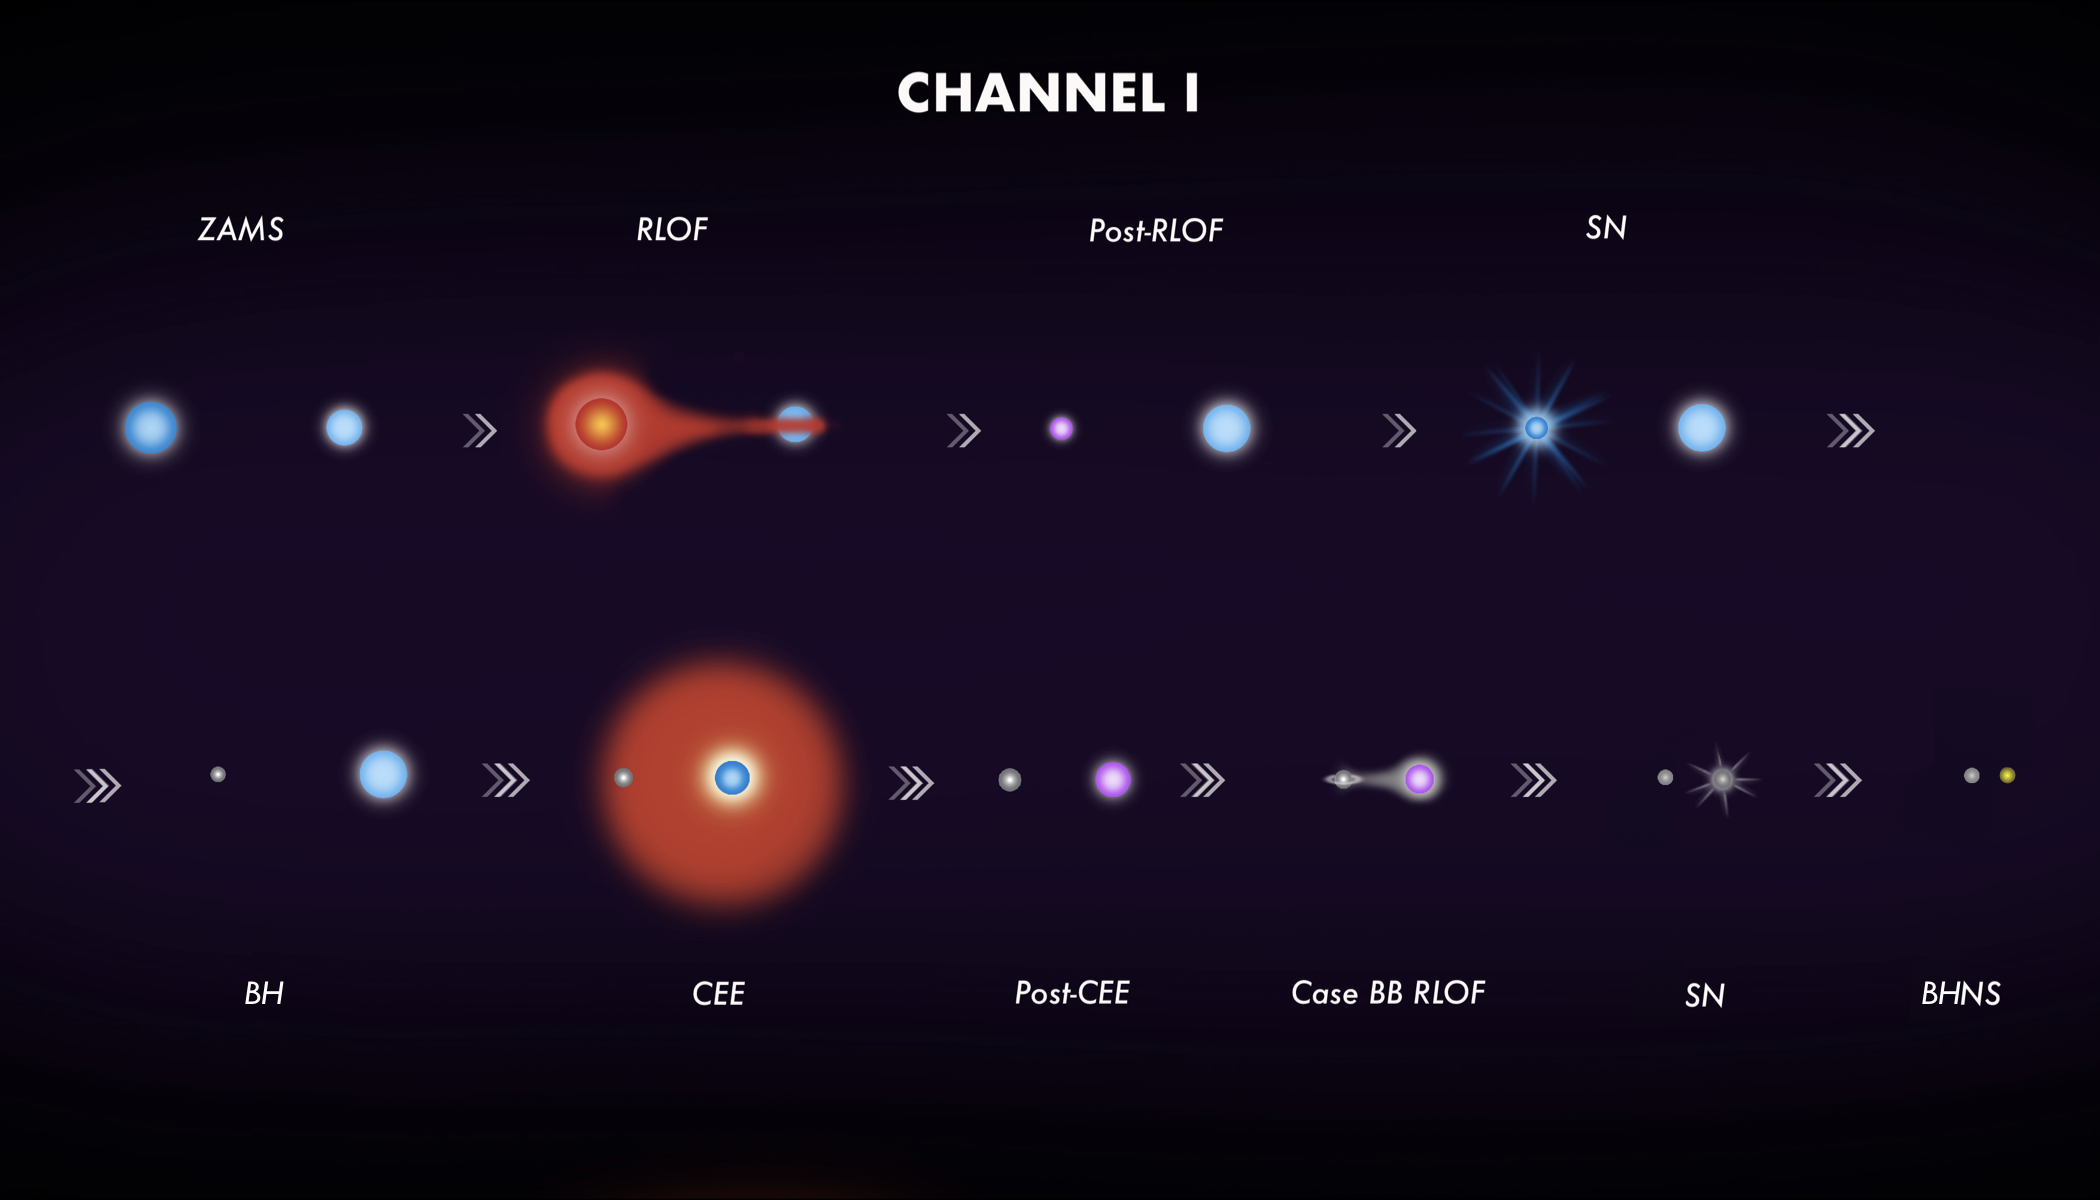
\includegraphics[width=1\textwidth]{../OtherImages/ClassicChannel}
   \caption{Schematic depiction of the classic formation channel as described in  Sect.~\ref{subsubsec:classic-channel}.  The acronyms are defined in the text.   The figure is based  on Fig~1. from \citet{2020arXiv200109829V} by T. Rebagliato, which is   \href{https://zenodo.org/record/3634498\#.XnS9ZC2ZNQI}{publicly available.} Adjustments to the original image made by S. Vinciguerra.}
    \label{fig:formation-channels-sketch}
%
\end{figure*}
%
%

In this section we describe the results of our population synthesis simulation for \bhnsSingle mergers for model \mAzero, which uses both our fiducial assumptions for the massive binary-star evolution (described in Section~\ref{subsec:method-BPS-assumptions} and Table~\ref{tab:population-synthesis-settings}) and our fiducial assumptions for the cosmic integration model  (see Table~\ref{tab-MSSFR-variations-labels}). 
We focus  on this model  to provide insight to a typical output of a \COMPAS simulation. 
This model choice is similar to earlier work done with {\COMPAS} and has been shown to match  the population of  \ac{NSNS} systems \citep{2018MNRAS.481.4009V} and the rate and mass distributions of the \ac{GW} sources \citep{2019MNRAS.490.3740N}.  



\subsection{Formation channels}
\label{subsec:bhns-BPS-formationChannels}
%

We identify four main groups of formation channels  described below. 
  The percentages, quoted in brackets after each header, indicate the fraction that each channel contributes to the total weighted number  of \bhnsSingle systems that  formed and merged in the Universe assuming the fiducial \ac{MSSFR} model. This is calculated using Equation~\ref{eq:MSSFR-merger-rate} and does not yet take into account the detection probability (which is discussed in Section~\ref{subsec:distributions-FIducial-GW-observable}). 
%   To calculate these percentages we average equally over the metallicity bins $Z_i$,  account for the sampling weight of each binary system in the simulation and normalize over the total rate of \bhnsSingle, given by $  \sum_i ( \rate_{\rm{form, c}}(\Zi)  /   \rate_{\rm{form}}(\Zi) )$, where $ \rate_{\rm{form, c}}$ is the \bhnsSingle formation rate for a given channel. \floor{iterate}
% \floor{numbers might still change a bit} 
%  The quoted percentages do not correspond to a physical occurrence rate of \bhnsSingle mergers in nature, as metallicities of stars in the Universe are not distributed following our grid points of  $Z_i$. \floor{do MSSFR weighting ? }
%  Nevertheless, we find that these quoted numbers are representative for the contribution of the channels in our later results (see Section \todo{X}) 
%  \floor{this is quite a long paragraph describing a nr that is not so important..?}. 
%
%The initial masses, separations and mass ratios for each channel are shown in Figure~\ref{fig:BHNS_ZAMSmasses}  for simulations with   $Z = 0.0142$ and  $Z = 0.001$ to represent, respectively,  solar metallicity (\citealt{2009ARA&A..47..481A}) and a low-metallicity environment. 
%

 
\subsubsection{(I) Classic channel (\PercentageStable)}
\label{subsubsec:classic-channel}
%
We find, in agreement with e.g., \citet[][]{2019MNRAS.490.3740N} for \ac{BHBH} mergers,  that the majority of the binaries  form a \bhnsSingle through the `classic'  formation channel where the binary experiences both a stable mass transfer and an unstable (CE) mass transfer phase. This classic channel is discussed in e.g. \citet[][]{1991PhR...203....1B,1973A&A....25..387V,2006csxs.book..623T,2008ApJS..174..223B} (see also \citealt{2018arXiv180605820M} and references therein). We schematically depict this formation channel in Figure~\ref{fig:formation-channels-sketch} and  describe it below in more detail for binaries that form a \bhnsSingle merger. \\
 %
 


The binaries in the classic channel are born with a wide range of initial separations  of  about $0.1$--$20$\AU  (see Figure~\ref{fig:BHNS_ZAMSmasses}). The initially most massive star (the primary) eventually expands and fills its Roche lobe initiating a mass transfer phase (Roche lobe overflow, RLOF) that is stable onto the initially less massive star (the secondary). This can either be case A, case B or case C mass transfer, 
%happen when the primary is at the end of the main sequence, is a Hertzsprung gap star, core helium burning star or post core helium burning star, 
leading to different sub-populations of binaries forming \bhnsSingle mergers. These sub-populations are particularly visible in the bottom left plot of Figure~\ref{fig:BHNS_ZAMSmasses} as the initial separation of the binary dominates the stellar type of the donor star at onset of the first mass transfer episode. Binaries in between those islands typically merge  before forming a \ac{DCO}, are disrupted during their evolution or instead form e.g., a \ac{NSNS} or BHBH. 
% 
 In our fiducial model the companion typically accretes a large fraction of   the mass that is lost from the primary star donor \citep[c.f.][]{2015ApJ...805...20S}.  Mass transfer typically ends when the donor has lost all of its hydrogen envelope.  The result for case A or B mass transfer is typically a stripped envelope star that is burning helium, which may be observed as a Wolf-Rayet star \citep{2007ARA&A..45..177C}.

Eventually, the stripped primary star ends its life in a \ac{SN}  and the first compact object, a \ac{BH} or NS, is formed. 
%This is typically a neutron star in our simulations, because of the low mass of the core of the progenitor. 
The binary needs to stay bound during the \ac{SN} to eventually form a \bhnsSingle. Typically, more than 80$\%$ of the binaries disrupts during the first \ac{SN} \citep[e.g.][]{2019A&A...624A..66R}, where disruption depends on the magnitude and orientation of the \ac{SN} kick, the separation of the binary and the amount of ejected mass (e.g., \citealt{1975A&A....39...61F,1983ApJ...267..322H,1998A&A...330.1047T,1999A&A...346...91B}).   
 
Later on, the secondary star also leaves the main sequence and expands to fill its Roche lobe.  This is the start of a reverse mass transfer phase from the secondary onto the compact object. 
 The extreme mass ratio at this moment in combination with an Eddington-accretion rate makes the mass transfer typically  non-conservative. This leads to a rapid hardening of the orbit faster than the radius of the secondary can respond as it loses mass. This leads the star to fill its Roche lobe even more as it loses mass,  resulting in dynamically unstable mass transfer and the start of a \ac{CE} event  \citep[e.g.][]{1997A&A...327..620S,2010ApJ...717..724G,2015ApJ...812...40G,2018MNRAS.481.4009V}.  During the \ac{CE} event  the separation of the binary rapidly decreases as the orbital angular momentum is lost to expel the CE.  If the \ac{CE} is ejected successfully, the result is a   close binary system consisting of a  \ac{BH} or \ac{NS} and a massive helium star.  Otherwise the system results in a merger of the star with the compact object, which can possibly form a  Thorne--{\.Z}ytkow object \citep{1977ApJ...212..832T}. %\floor{write fraction of successfull/ unsuccessfull?}
 
In a subset of the binaries there is a stable case BB  mass transfer phase after the \ac{CE} from the helium star onto the primary compact object.  This typically occurs when the secondary is a relatively low mas helium star as they expand to larger radii compared to more massive helium stars in the single star prescriptions of \citet{2000MNRAS.315..543H} implemented in \COMPAS (although  \citealt{2020arXiv200301120L}  point out that these prescriptions might underestimate  the stellar radii expansion of helium stars especially at lower metallicities, $Z \approx 0.001$). 

The helium star eventually forms a \ac{NS} or BH in the second \ac{SN}.   If the binary stays bound, a \bhnsSingle  binary is formed that gradually decays in separation under the emission of gravitational waves.  If the separation is small enough (typically $<10$\Rsun, see Figure~\ref{fig:BHNS_DCOmasses}) the \bhnsSingle will merge within \thubble.  
 
%
\subsubsection{(II) Only stable mass transfer channel (\PercentageBnoCE)}
%
In  about \PercentageBnoCE{}  of all  mergers the binary forms  similar to the classic channel (I) but does not experience an unstable mass transfer phase leading to a \ac{CE}. 
This channel thus only has  stable mass transfer phases    (c.f., \citealt[][]{Heuvel:2017sfe, 2019MNRAS.490.3740N}, see also e.g., \citealt[][]{2017MNRAS.465.2092P}). 
To still form  \bhnsSingle systems with semi-major axis $\lessapprox 10$\AU that can merge in \thubble, these  binaries typically experience a second stable mass transfer phase after the first  \ac{SN} from the secondary star onto the compact object that decreases the separation of the binary. 



\subsubsection{(III) Single-core \ac{CE} as first mass transfer   channel (\PercentageImmediateCE)}
%%%%%% CHANNEL UNSTABLE CASE C %%%%%%%%%%
%
In a tight window of initial separations ($\sim 10$\AU), the first mass transfer phase leads to an unstable single-core \ac{CE} event,  with only the donor star having a clear core-envelope structure.  The donor star in the \ac{CE} is typically a core helium burning star or a star on the giant branch. If the \ac{CE} is successfully ejected this leads to a tight binary star system. The primary star will eventually form a \ac{BH} in a \ac{SN}. From this moment the evolution follows Figure~\ref{fig:formation-channels-sketch} from the post-CE step: there is a case BB mass transfer phase onto the \ac{BH} after which the secondary eventually forms a \ac{NS}. In this formation channel the \ac{BH} always forms first. 

%
\subsubsection{(IV) double-core CE  as first mass transfer  channel  (\PercentageDCCE)}
%
In this channel the primary star fills its Roche lobe when both stars are on the giant branch and both stars  have  a core-envelope structure. The mass transfer is  unstable, leading to a double-core CE.  Both stars need to evolve on a similar timescale and, therefore,  have similar initial masses (i.e. $ \qi \sim 1$) as can be seen in the bottom panel of Figure~\ref{fig:BHNS_ZAMSmasses}. The further evolution of the binary proceeds similar to channel III, except that in most cases there is no case BB mass transfer phase and the \ac{NS} can also form first. 
This channel is similar to the channel described by \citet{1995ApJ...440..270B,1998ApJ...506..780B} and  later on \citet{Dewi:2006bx}.  \\
%

% The channels and fractions mentioned above roughly match with findings by \citet{2018MNRAS.481.1908K}


%
\begin{figure*}
\includegraphics[width=\textwidth]{../PlottingScripts/3_DCO-Population/BHNS_InitialParam.png}
   \caption{Initial parameters of binaries forming \bhnsSingle systems  that merge in a Hubble time for a binary population synthesis simulation with our fiducial model \mAzero  (see Section.~\ref{sec:method}) for metallicities $\Zi=0.001$ (left panels) and $\Zi=0.0142$ (right panels). Colors represent different formation channels, described in Section~\ref{subsec:bhns-BPS-formationChannels}. Each point represents one simulated binary system that lead to a \bhnsSingle merger. The areas of the points represent the statistical weight $w_{\rm{i}}$ (i.e. probability of occurrence)  of that binary in our simulation.  Dotted lines indicate some values of the parameters to guide the reader. }
   %
    \label{fig:BHNS_ZAMSmasses}
\end{figure*}
%   


%%%% FIGURE WITH FINAL BHNS PARAMETERS
\begin{figure*}
%
\includegraphics[width=\textwidth]{../PlottingScripts/3_DCO-Population/BHNS_FinalParam.png}
%
   \caption{Same as Figure~\ref{fig:BHNS_ZAMSmasses} but now for the final parameters  at \tDCO, the moment of the \ac{DCO} formation.  
%   \textbf{[top panels:]}  
%   \ac{NS} mass versus \ac{BH} mass of the \bhnsSingle binaries. 
   The gray areas  in the top panels denote the \ac{DCO}s that have final masses such that the \ac{NS} is tidally disrupted  outside the  \ac{BH} when assuming a \ac{NS} radius of 11.5\km or 13\km and  \ac{BH} spins of  $\chibh = 0$ or $0.5$ (based on  \citealt[][]{2018PhRvD..98h1501F}). 
%    \textbf{[bottom panels:]} 
%   eccentricity  versus semi-major axis of the \bhnsSingle binaries.
   The dashed black lines in the bottom panels show lines of constant $\tinspiral \in \{ 1000\yrs, 1\Myr, 1\Gyr,  \thubble \}$. 
   To calculate the period of the \bhnsSingle and the lines of constant inspiral time we assumed $\mbhf=10\Msun$ and  $\mnsf=1.4\Msun$.  } %  using \citet{1964PhRv..136.1224P}. 
%
  \label{fig:BHNS_DCOmasses}
\end{figure*}
%




%
\subsection{Initial properties \bhnsSingle mergers}
\label{subsec:bhns-BPS-ZAMSm1m2}
%

The locations  in the initial parameter space of the binaries (e.g.,  masses, mass ratios, and separations)  leading to the formation of a \bhnsSingle system that merges in a Hubble time are shown in Figure~\ref{fig:BHNS_ZAMSmasses}  for metallicities $\Zi=0.001$ and $\Zi=0.0142$, which represent respectively a low and solar \citep{2009ARA&A..47..481A} metallicity environment. 

As can be seen in the top panels of Figure~\ref{fig:BHNS_ZAMSmasses},  the majority of \bhnsSingle merger at metallicity $\Zi=0.001$ originate from binaries with  masses  $10 \leq $ \monei/\Msun $\leq 60$ and   $10 \leq $\mtwoi/\Msun $\leq 25$, whilst at solar metallicity this shifts to  $30 \leq $ \monei/\Msun $\leq 150$ and $13 \leq $\mtwoi/\Msun $\leq 25$ respectively. Higher metallicities correspond to stronger line-driven stellar winds, which lead to more mass loss in stars and lower mass carbon-oxygen cores compared to the same stars born at lower metallicities. These lower carbon-oxygen cores typically leave behind compact remnants with lower masses, and can therefore instead form \ac{NSNS} systems (compared to \bhnsSingle at lower metallicity). Subsequently, to make \bhnsSingle mergers, stars in  binaries at higher metallicities have to initially be more massive compared to binaries at lower metallicities. 

%The locations  in the initial parameter space of the binaries (e.g. their masses, mass ratios, and separations)  that lead to the formation of a \bhnsSingle system that merge in a Hubble time depend strongly on the metallicity. This is shown in Figure~\ref{fig:BHNS_ZAMSmasses} that shows the most important initial parameters of the mergers in our fiducial simulation for $Z=0.001$ and $Z=0.0142$ . 


\bhnsSingle mergers originate from mass ratios $0.2 \leq \qi \leq 1$ and $0.1  \leq \qi  \leq 0.6$ for  $\Zi=0.001$ and $\Zi=0.0142$ (see bottom panels  Figure~\ref{fig:BHNS_ZAMSmasses}).  
At higher metallicity, \bhnsSingle mergers typically come from only more extreme mass ratios as stronger stellar winds will equalize the more extreme mass ratio before the onset of mass transfer, making the mass transfer more stable and the system more likely to survive to form a \ac{GW} progenitor. 
%This is because at higher metallicities, stars self-strip more mass due to stronger stellar winds. This mass loss leads binaries starting initially with unequal (equal) mass ratios to typically becoming more equal (unequal) at the onset of the first mass transfer, compared to lower metallicities. Equal masses in the binary lead more often to stable mass transfer as the stability criteria is determined based on whether  the rate at which the accreting star can accept mass is  larger or similar to the rate at which the donor is losing mass, which is for evolved stars typically the thermal (Kelvin-Helmholtz) timescale. If the mass ratio is closer to one at the onset of mass transfer, the secondary is more likely to satisfy this criteria,   leading to stable mass transfer and survival of the system. All in all, this leads to \bhnsSingle mergers originating from initially more extreme mass ratios at higher metallicities. 

The initial separation of the binaries forming \bhnsSingle mergers spans the range $0.1 \leq \ai   \leq 25$\AU  with higher metallicity favoring slightly larger initial separations.  
The latter seems counter-intuitive, but comes from  subtle and indirect effects of the wind loss being stronger at higher metallicities.
As discussed above, the binaries at higher metallicities originate from initially more massive primary stars in the range $25$--$150$\Msun.  The radii of these stars typically expand more during the Herzprung-gap phase (case B mass transfer) in the stellar evolution tracks implemented in {\sc{COMPAS}}. For example, the most massive primary stars forming a \bhnsSingle expand
to approximately $2200\, (700)$\Rsun at $\Zi=0.0142\,$ $(\Zi=0.001)$.% (see Appendix~\ref{sec:app-radii-as-function-of-Z}). 
Since this expansion in combination with the initial separation determines when mass transfer happens, the binary needs to have a much larger initial separation at $\Zi=0.0142$ to form through the same channel as a binary with smaller separation at $\Zi=0.001$.
In addition,  the secondary star is typically more massive at the onset of a \ac{CE}, causing the binary to shrink more compared to lower metallicity binaries. 

The combination of effects described above cause almost all binaries at $\Zi=0.0142$ to form through just two formation channels: the classic channel and the channel with only stable mass transfer. This is in  agreement with \citet[][see their Table C1]{2018MNRAS.481.1908K}. 








\begin{table}[]
\caption{Properties of the \bhnsSingle at the moment of \ac{DCO} formation. In this Table, we list the symbols and units for each parameter, as well as the figure where the parameter is presented.}
\label{tab:properties_variables}
\resizebox{\columnwidth}{!}{%
\centering
\begin{tabular}{llll}
\hline
\hline
Property		 	& Symbol & Units  \\ \hline % & Figures 
\ac{BH} mass 	& \mbhf          	&     \Msun   \\%		       &   \ref{fig:BHNS_DCOmasses}, \ref{fig:BHNS_ObservableDistributions_per_metallicity}, \ref{fig:BHNS_DCO_observed}      \\
\ac{NS} mass 	& \mnsf				&      \Msun \\%		       &   \ref{fig:BHNS_DCOmasses}, \ref{fig:BHNS_ObservableDistributions_per_metallicity}, \ref{fig:BHNS_DCO_observed}              \\
Total mass 		& \mtotf          	&      \Msun 	 \\%	       &   \ref{fig:BHNS_ObservableDistributions_per_metallicity}, \ref{fig:BHNS_DCO_observed}               \\
Chirp mass  		& \mchirpf        	&       \Msun	 \\%	       &   \ref{fig:BHNS_ObservableDistributions_per_metallicity}, \ref{fig:BHNS_DCO_observed}          \\
Mass ratio  		& \qf        			&        -			 \\%	       &    \ref{fig:BHNS_ObservableDistributions_per_metallicity}, \ref{fig:BHNS_DCO_observed}          \\
Inspiral time 		& \tinspiral         &        \Gyr	 \\%	       &   \ref{fig:timescalesEvolution}, \ref{fig:BHNS_ObservableDistributions_per_metallicity}, \ref{fig:BHNS_DCO_observed}          \\
Semi-major axis&	\af      			&        \AU		 \\%	       &   \ref{fig:BHNS_DCOmasses}, \ref{fig:BHNS_ObservableDistributions_per_metallicity}, \ref{fig:BHNS_DCO_observed}          \\ 
Eccentricity		&	\ef      			&        -			    \\ \hline \hline %     &   \ref{fig:BHNS_DCOmasses}, \ref{fig:BHNS_ObservableDistributions_per_metallicity}, \ref{fig:BHNS_DCO_observed}          \\ \hline \hline
\end{tabular}%
}
\end{table}

%From left to right and up to down:    the \ac{BH} mass \mbhf, \ac{NS} mass \mnsf, mass ratio \qf = / ,  inspiral time, total mass nd chirp mass


\subsection{Final properties of  \bhnsSingle mergers  }
\label{subsec:bhns-BPS-DCOmasses}
%
%

%
%%%% FIGURE WITH METALLICITY DISTRIBUTIONS: 
\begin{figure*}
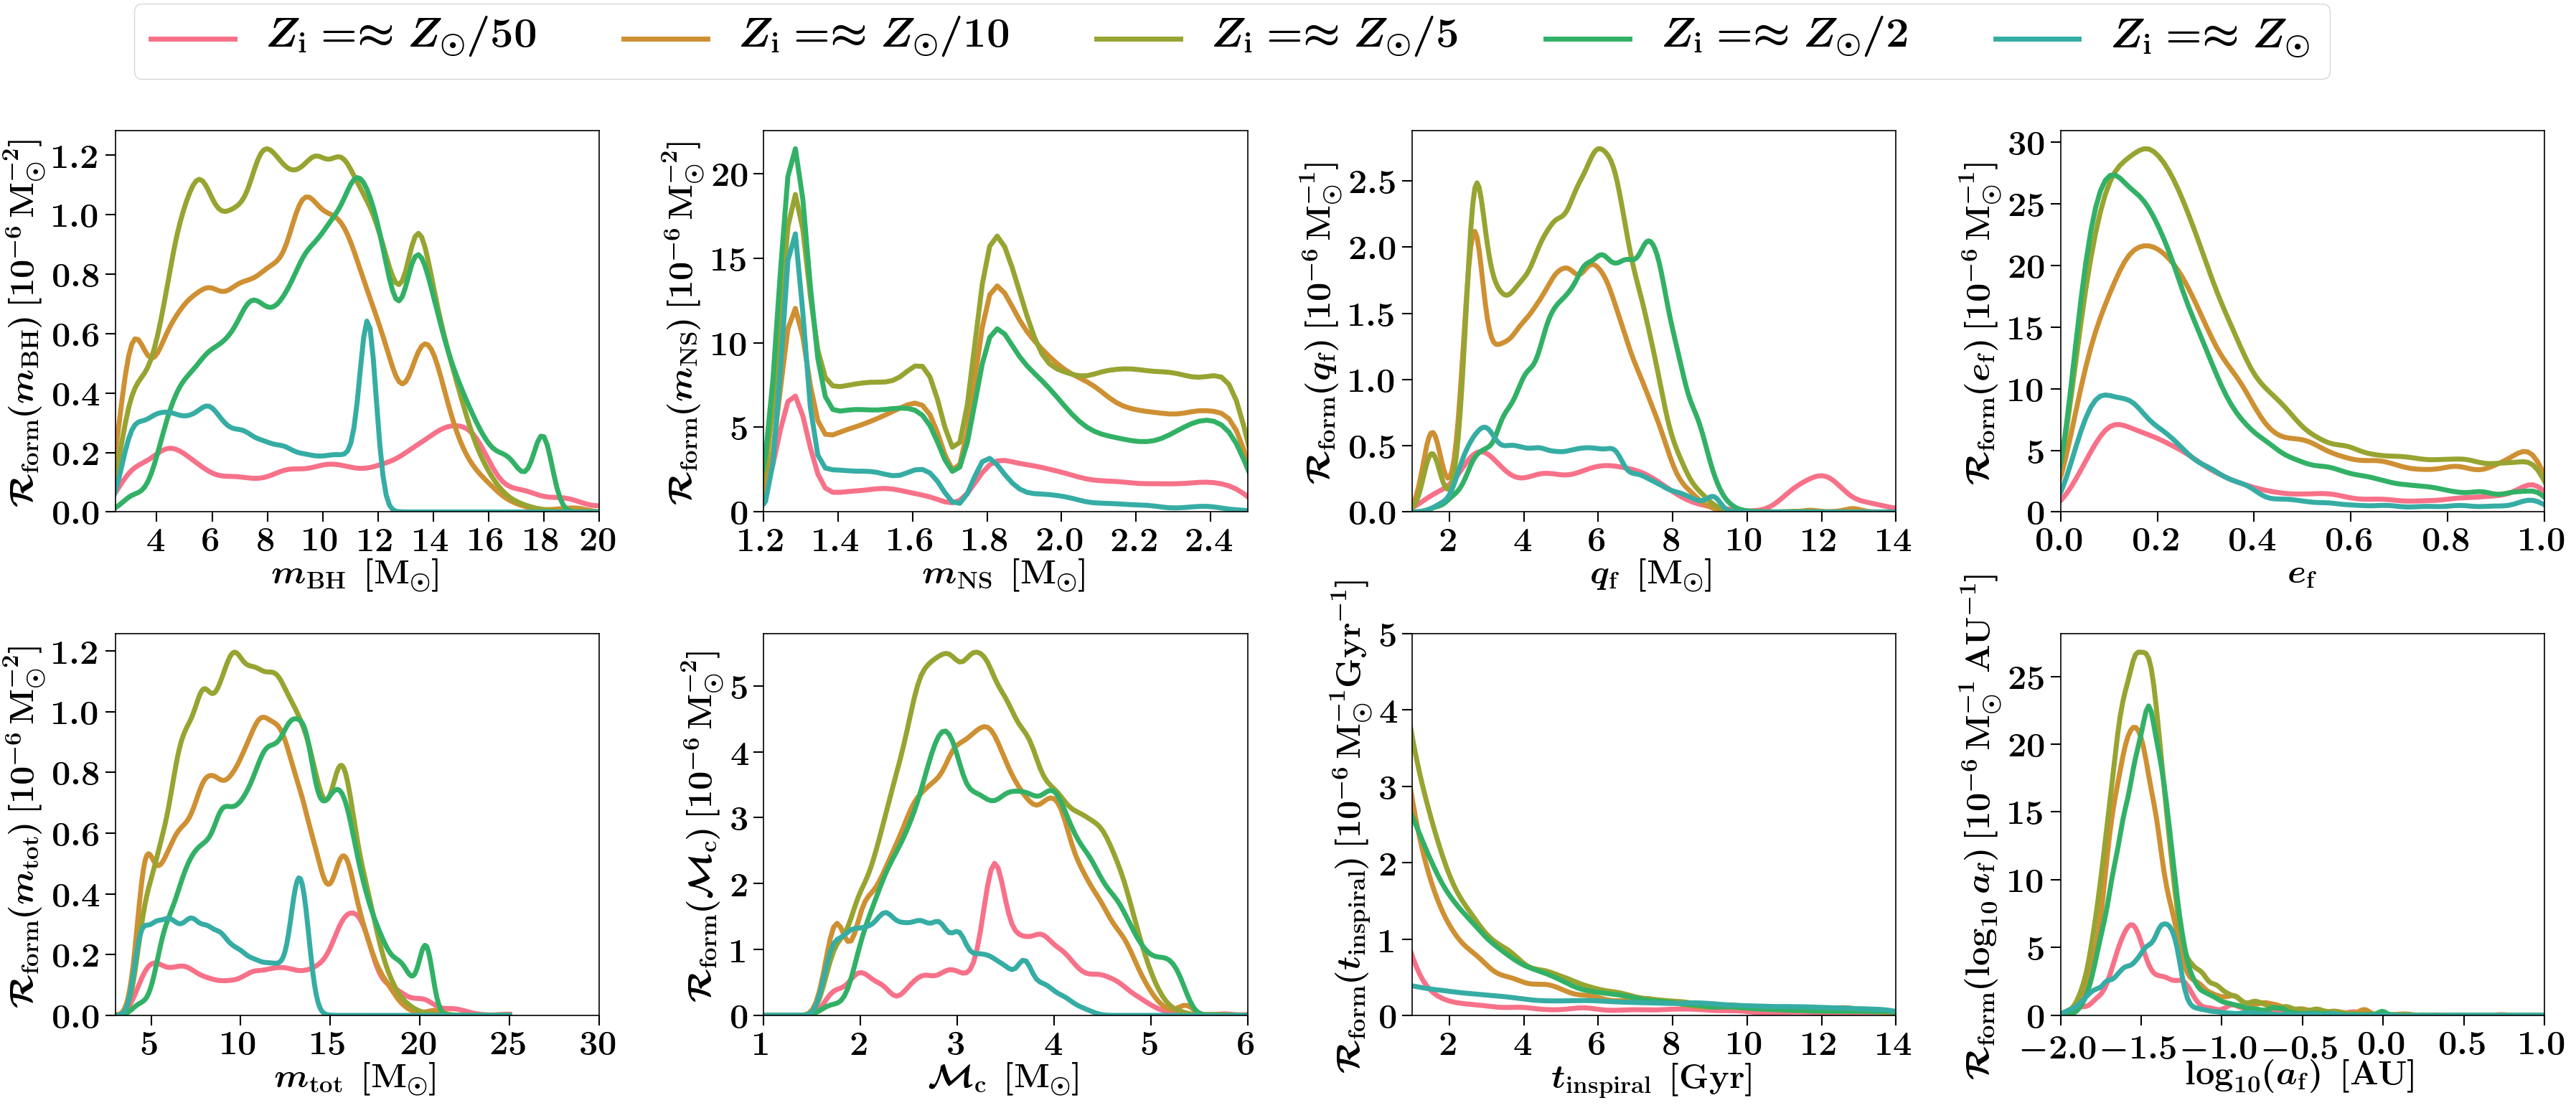
\includegraphics[width=1\textwidth]{../PlottingScripts/3_DCO-Population/CombinedZdistributions_horizontal.png}
   \caption{ Distributions of the characteristics of \bhnsSingle systems that merge in a Hubble time at the moment after the second  \ac{SN} for five different metallicities $\Zi$.  The yield is calculated using Equation~\ref{eq:formation-rate-COMPAS} and plotted using a weighted kernel density estimator with a kernel bandwidth of 0.01. We use the short hand notation $\mathcal{R}_{\rm{form}}(x)  \equiv  {\rm{d}}N /({\rm{d}}M_{\rm{SFR}} {\rm{d}}x) $ for variable $x$. The variables are given in Table~\ref{tab:properties_variables}. }
  \label{fig:BHNS_ObservableDistributions_per_metallicity}
\end{figure*}
%



The final characteristics of the \bhnsSingle systems at  \tDCO (after the second \ac{SN}) are shown in Figure~\ref{fig:BHNS_DCOmasses}. 
In addition, Figure \ref{fig:BHNS_ObservableDistributions_per_metallicity} shows the weighted histogram distributions (i.e. the yield of  \bhnsSingle mergers) for five different simulated metallicities \Zi  for typical \bhnsSingle characteristic at \tDCO.  
% that depicts the properties of the \bhnsSingle systems that merge in a Hubble time at the moment after the second \ac{SN} when the \ac{DCO} forms. 

%top panels of Fig~\ref{fig:BHNS_DCOmasses} show that
The   \bhnsSingle mergers have \acp{NS} with masses in the range $1.25 \leq \mnsf/\Msun \leq 2.5$ (where the maximum \ac{NS} mass is set to 2.5\Msun in our fiducial model). 
The discontinuity in the \ac{NS} remnant mass around 1.7\Msun is a result from the discontinuity in the proto-compact object mass equation at carbon-oxygen cores of $M_{\rm{CO}}= 3.5$\Msun  in the delayed \ac{SN} remnant mass prescription (Equation~18 in  \citealt{2012ApJ...749...91F}), see also Appendix~\ref{sec:app-Fryer-bug-fix} for more details. 
The over-density of remnant masses around $1.25\Msun$ comes from the  \ac{ECSN} and \ac{USSN} prescriptions that map many stars to a small mass range around 1.25\Msun  (see Section~\ref{subsec:method-BPS-assumptions} and \citealt{2018MNRAS.481.4009V}). 
 



	 The \acp{BH} in the \bhnsSingle binaries have masses in the range  $2.5 \leq \mbhf/\Msun \leq 20$ and $2.5 \leq \mbhf/\Msun \leq 12$ for metallicities  $Z=0.001$ and  $Z=0.0142$, but the \ac{BH} can extend to \mbhf $\approx 25$\Msun for extreme metallicities of \Zi $=0.0001$ as seen in the top left panel of Figure~\ref{fig:BHNS_ObservableDistributions_per_metallicity}. 
	 We find that \bhnsSingle binaries with \ac{BH} masses above 15\Msun are rare in agreement with e.g., \citet{2020arXiv200302277R}. 
At lower metallicities \bhnsSingle mergers are formed with more massive \acp{BH} compared to higher metallicities, as can be seen in the distributions of \mbhf, \qf,  \mtotf and  \mchirpf in Figure~\ref{fig:BHNS_ObservableDistributions_per_metallicity} that are more extended to higher masses for lower metallicities. 
This is because stars at lower metallicities lose less mass during their lives through  line-driven stellar winds leading to larger remnant masses.  

The delayed  \ac{SN} remnant mass prescription that we use does not force a \ac{BH} mass gap between $2.5$--$5\Msun$ and we therefore find \acp{BH} with masses close to the maximum \ac{NS} mass of $2.5\Msun$ as can be seen in Figures.~\ref{fig:BHNS_DCOmasses}  and \ref{fig:BHNS_ObservableDistributions_per_metallicity}. 

The over-density of BHs with remnant masses around $12\Msun$ in Figure~\ref{fig:BHNS_DCOmasses} is due to our prescription of LBV wind mass loss that maps a broad range of initial ZAMS masses to the same carbon-oxygen core masses and hence the same \ac{BH} remnant masses (see for more details Appendix B of  \citealt{2019MNRAS.490.3740N}). 
This also results for other metallicities in peaks in the \ac{BH} mass distribution around the highest \ac{BH} mass for that metallicity as can be seen in Figure~\ref{fig:BHNS_ObservableDistributions_per_metallicity}. 

%For  37$\%$(63$\%$) and 26$\%$(56$\%$), for respectively $Z=0.001$ and $Z=0.0142$  our \bhnsSingle mergers have final mass ratios that do not exceed $q_{\rm{final}} = m_{\rm{BH}} /  m_{\rm{NS}} = 3\, (5)$. 
A subset of the \bhnsSingle mergers in our fiducial simulation have  final masses such that the \ac{NS} disrupts outside of the \ac{BH} during the merger.  
%This is shown in Figure~\ref{fig:BHNS_DCOmasses} for respectively assuming a \ac{NS} radius and fixed spin for all \acp{BH} of: $(R_{\rm{NS}}, \chibh) \in [(11.5,0), (13,0), (11.5, 0), (13, 0.5)]$, where the \ac{NS} radius is in \km (see also Section~\ref{subsec:method-tidal-disruption-BHNS}).
In general it can be seen that only low mass \acp{BH} and low mass \acp{NS} result in a tidal disruption of the \ac{NS}. For higher \ac{BH} spins and less compact \acp{NS} more \acp{NS} in \bhnsSingle mergers will be tidally disrupted. 
  The fractions of \bhnsSingle mergers that are tidally disrupted  are approximately  $[4\%, 9\%, 19\%, 34\%]$  and $[20\%, 36\%, 48\%, 59\%]$ for $\Zi = 0.001$ and $\Zi = 0.0142$ for \ac{NS} radii and \ac{BH} spins $(R_{\rm{NS}}, \chibh) \in [(11.5,0), (13,0), (11.5, 0), (13, 0.5)]$.

%\ac{NS} disruptions in \bhnsSingle mergers could potentially be observed  as electromagnetic counterparts to \bhnsSingle \ac{GW} observations such as a kilonova or short gamma-ray burst. 
%The values $\qf = 3\, (5)$ are approximate and based on Figure~5 from \citet[][]{2018PhRvD..98h1501F} when assuming a $1.35$\Msun \ac{NS} with a radius of $13$\km. 
%The exact mass ratios at which a NS gets disrupted and the amount of matter that is ejected strongly depend on e.g. the assumed \ac{NS} equation of state  \citep{2011ApJ...727...95P, 2012PhRvD..86l4007F,2018PhRvD..98h1501F}, see for more details Section~\ref{subsec:method-tidal-disruption-BHNS}. 




%
%  This could potentially lead to an electromagnetic counterpart accompanying the merger. GRMHD simulations have shown that this happens for final mass ratios below about 0.3. We mark this area in Figure~\ref{fig:BHNS_DCOmasses} with a gray hashed line. On the other hand, a \ac{NS} in a \bhnsSingle merger that has a final mass ratio larger than about 0.3 will be completely swallowed by the \ac{BH} before being tidally disrupted. The critical final mass ratio for which a \ac{NS} can be tidally disrupted outside of the \ac{BH} innermost-stable orbit depends on the equation of state of the \ac{NS} and the spin of the BH. We describe in Sect.~\ref{sec:bhns-EjectedMass} a more detailed discussion on the properties of electromagnetic counterparts in our simulations.

%Mergers of BH-NS binaries (always resulting in a \ac{BH} as
%the resulting compact remnant) are expected to be accom- panied by the formation of an hyperaccreting disk only if the mass ratio between the \ac{BH} and \ac{NS} does not exceed the value ∼ 3−5, with the precise value depending on the equa- tion of state of the \ac{NS} and the \ac{BH} spin (Pannarale et al. 2011; Foucart 2012; Foucart et al. 2018). (see e.g. Bartos et al. 2013 for a review)


%[x_eccentricities_thousandYr,x_eccentricities_toneMyr, x_eccentricities_tGyr, x_eccentricities_tHubble]
 \bhnsSingle binaries that merge in a Hubble time typically have merger times in the range $1\Myr \leq t_{\rm{merge}} \leq \thubble$ at the moment of the \bhnsSingle formation, corresponding with semi-major axis between $1 \leq \af / \Rsun  \leq 100$,  as can be seen in the bottom panels of Figure~\ref{fig:BHNS_DCOmasses}. 
 Systems with larger semi-major axis still merge in a Hubble time if the binary is more eccentric as this decreases the inspiral time. 

A fraction of $\sim 1\%$ of the \bhnsSingle systems in the $Z=0.001$ simulation  forms with $t_{\rm{merge}} \sim  10^3\,$\yrs. 
These binaries form through the classic channel with stable case B mass transfer at the first mass transfer.
 The \ac{NS} eventually forms first and there is a reversed case BB mass transfer phase from the secondary onto the \ac{NS}. 
 This hardens the binary to a semi-major axis of  $\lesssim 1\Rsun$.
   These binaries can be of astrophysical significance as the mass transfer   onto the \ac{NS} can spin up the \ac{NS} due to the exchange of angular momentum \citet[e.g.,][]{1994MNRAS.269..455J,2008MNRAS.388..393K}, leaving behind a very tight millisecond-pulsar -- \ac{BH} system with short merger times. Moreover,  in such tight systems the stripped helium star can also tidally spin up, forming a highly spinning \ac{BH} (similar to e.g., \citealt{2016MNRAS.462..844K,2018MNRAS.473.4174Z,2020A&A...636A.104B,2018A&A...616A..28Q,2019arXiv190612257B}). Such binaries with  short delay times and $\chi_{\rm{eff}} >0$ could be distinguished with \ac{GW} observations  \citep{2018PhRvD..98d3002Z} or radio surveys \floor{REF?}.
    In addition, this subset of binaries with extremely short merger times and low mass \acp{BH} could be candidates for early r-process enrichment (c.f.. \citealt{2019ApJ...872..105S,2019arXiv191013436A, 2019ApJ...886....4Z}).



%The total yield of \bhnsSingle mergers peaks around \Zi $\sim 0.002$ as also discussed in the next section.  
%

%
%
\begin{figure*}
%   
    \centering
    \subfloat[]{{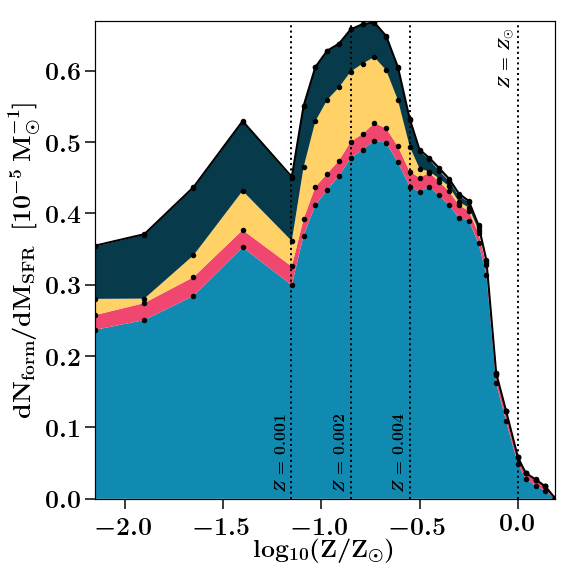
\includegraphics[width=1.0\columnwidth]{../PlottingScripts/3_DCO-Population/channelBHNS_pessimistic_small_4channels.png} }}%
    \qquad
    \subfloat[]{{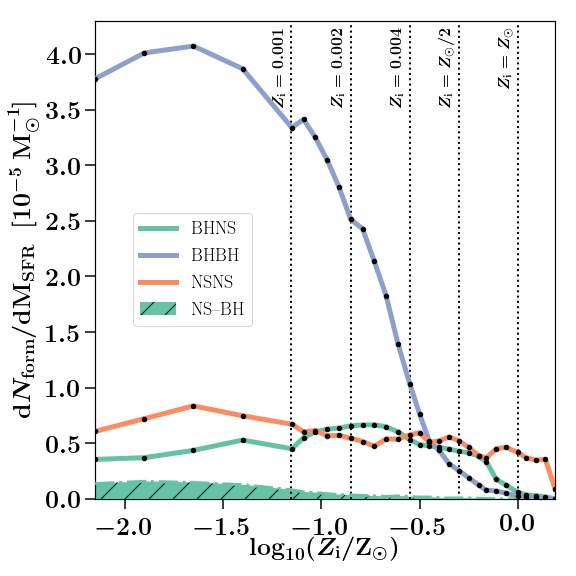
\includegraphics[width=1.0\columnwidth]{../PlottingScripts/3_DCO-Population/Rate_vs_Z_pessimistic_Fiducial.png} }}%
      \qquad
%    \caption{2 Figures side by side}%
   \caption{Number of double compact object mergers with  delay times $\tdelay \leq \thubble$  that form per unit star forming mass  (\MSFR) per  metallicity $\Zi$ in our fiducial model.  The left panel shows the \bhnsSingle rate with colours indicating the contribution of each formation channel (discussed in Section~\ref{subsec:bhns-BPS-formationChannels}). The right panel shows the  double compact object rates for BHNS,  \ac{BHBH} and \ac{NSNS}  mergers. The green hashed area shows the subset of \bhnsSingle mergers where the \ac{NS} forms in the first SN.    The 30 black scatter points denote the simulated \Zi.}
  \label{fig:BHNS_rate_per_metallicity}
\end{figure*}
%





%\subsection{Characteristic \bhnsSingle merger distributions as function of metallicity}
%
%%%%%%%
%
%The typical trends in metallicity are also visible in  Figure~\ref{fig:BHNS_ObservableDistributions_per_metallicity}, which shows histograms of the yield of  \bhnsSingle mergers for five different simulated metallicities \Zi  for typical \bhnsSingle characteristic at the moment after the second  \ac{SN} when the binary has formed the \bhnsSingle system (i.e. \tDCO). 
%
%At lower metallicities \bhnsSingle mergers are formed with more massive \acp{BH} compared to higher metallicities, as can be seen in the distributions of \mbhf, \qf,  \mtotf and  \mchirpf that are more extended to higher masses for lower metallicities.  
%This is because at lower metallicities stars have less strong line-driven winds and keep more of their envelope mass. % (see also Section~\ref{subsec:Metallicity-dependent-merger-rate-Rform}).
%There is typically a double peak in the  \ac{BH} mass distributions, with one of the peaks  around the righter most edge of the distribution. This is because our LBV wind mass loss prescription maps a range of massive stars that enter the Humphreys-Davidson limit  to the same \ac{BH} remnant masses. This is also seen in \citet{2010ApJ...714.1217B, 2015ApJ...806..263D, 2019MNRAS.490.3740N}. 






%This causes a double peak behavior in the total mass and chirp mass and mass ratio. 
%The mass ratio shows that most binaries have a more extreme mass ratio, caused by the \ac{BH} being more massive than the typical NS. However, in $X\%$ of the systems, the mass ratio is smaller than $1/3,( 1/5$), which are possible candidates to produce also  ejecta as the \ac{NS} is disrupted outside of the \ac{BH} innermost-stable-orbit. We find longer tails near equal mass ratios (compared to Figure9 Dominik 2012). This is both because our fiducial delayed prescription allows lower mass BHs, making it possible to have smaller mass ratios and because our large number of \bhnsSingle recovers more likely such tails of distributions. 





%%\floor{FLOOR TO DO: try to find trends in channels or \ac{NS} or \ac{BH} first (eccentricity prob depends on  \ac{SN} natal kick, which depends on \ac{NS} \ac{BH} first and USSN vs ccSN) -- so far checks didnt find any clear trends}
%

%\subsection{Formation order of double compact objects}
%\label{subsec:bhns-BPS-BHNSvsNSBH}
%\begin{figure*}
%%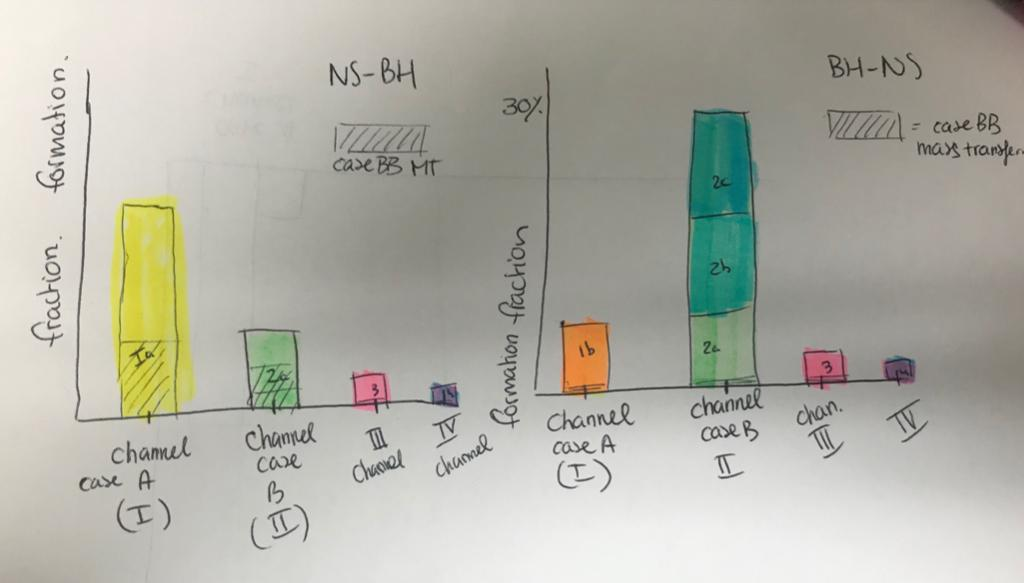
\includegraphics[width=\textwidth]{../PlottingScripts/3_DCO-Population/possibleFIG}
%   \caption{Possible fig to show BH--NS vs NS--BH fractions and to show ultra-stripped SN fraction}   
%  \label{fig:BHNSotherProperties}
%\end{figure*}




%%
%\subsection{BH--NS vs NS--BH }
%In our simulation $55\%$ ($45\%$) of the mergers are a  BH--NS  (NS--BH). The relative percentages between the two types of mergers changes between the formation channels and are shown in Figure~\ref{fig:BHNSotherProperties}. Our stable case A mass transfer channel always forms a NS--BH merger unless the second star explodes first (Ib, SN2 first). The other channels typically form a BH--NS system. 
%
%%The stable case A mass transfer channel always forms NS--BH mergers as the primary has transferred  a substantial amount of mass onto the secondary such that the primary forms the least compact object. In the stable case B mass transfer case $75\%$ of the binaries forms a BH--NS and only $25\%$ of the cases the \ac{NS} forms first. In the other channels the \ac{BH} forms first in $80\%$ of the cases (versus $20\%$ of the cases the \ac{NS} forming first). 
%
%% The number of NS--BH systems is strongly dependent on the stability and conservativeness assumptions of the mass transfer phase. This is because the initially less massive star has to accrete a substantial amount of mass from the primary star  in order to form the more massive compact object in the NS--BH binary,  even though it was initially less massive than the primary star. Similarly, the primary has to loose a substantial amount of mass to form the \ac{NS} in these NS--BH mergers.
%
%The formation order of the BH--NS and NS--BH systems is particularly interesting for the formation of millisecond-pulsar black hole binaries. In such systems the \ac{NS} is thought to spin up to a millisecond-pulsar by stable accretion through Roche Lobe overflow from the companion star onto the NS. This is only possible if the \ac{NS} forms first. Such systems would be extremely interesting for tests of GR \floor{REFs}.  A further discussion on this is in Section~\ref{sec:bhns-EjectedMass}.
%





%
%\subsection{Ultra-stripped second SN}
%\label{subsec:bhns-BPS-USSN}
%%
%The secondary star typically initiates the \ac{CE} phase after the primary star has formed a compact object. If the \ac{CE} is successfully ejected, the binary now consists of a stripped helium star with a compact object. Depending on the orbital separation and the radius of the stripped-helium star, the  star can fill its Roche lobe and initiate a second phase of mass transfer onto the compact object (Case BB Roche-lobe overflow). As the compact remnant accretes  at an Eddington limited rate, most of the donated mass is typically lost through jets from the binary system. This generally leads to shrinking of the orbit. In addition, the mass transfer can spin up the compact remnant and ultra-strip the donor star. This leads to an ultra-stripped star that later explodes as an ultra-stripped  \ac{SN} (Tauris et al. 2013, 2015 etc. ). 
%
%We find that a fraction $X\%$ of our \bhnsSingle mergers experiences an ultra-stripped SN. The relative fractions per channel are shown in Fig~\ref{fig:BHNSotherProperties}. Almost all ultra-stripped  \ac{SN} occur in binaries forming a BH--NS merger. In those binaries the \ac{BH} forms first and so the naked-helium star is the star that will form the \ac{NS} in the binary. The mass of these NS-progenitor naked-helium stars are typically lower compared to the helium star in the NS--BH binary that  form the BH. Lower mass helium stars are thought to expand more in radii during their evolution. As a result the NS-progenitor stars are more ikely to fill their Roche lobe and initiate a case BB mass transfer phase. More recent studies by (Laplace et al. 2019) show that more massive naked-helium stars might expand more, but this is not taken into account in our models. 
%



%\section{to discuss:}
%Even the mass of BHs in merging NSBHs does not change significantly with time (see the left-hand panel of Figure 5). Again, this originates from the fact that the merger effi- ciency of NSBHs born from metal-poor progenitors is orders of magnitude higher than the merger efficiency of NSBHs born from metal-rich progenitors (see Giacobbo & Mapelli 2018).
%Light BHs are more frequent than massive BHs in NS- BHs: most BHs in merging NSBHs have mass ≤ 10 M⊙, regardless of the merger time. The dearth of massive BHs is particularly strong in the case of run CC15α5.
%From the right-hand panel of Figure 5, we see that mas- sive neutron stars (NSs, mNS > 1.4 M⊙) are more com- mon than low-mass NSs in NSBHs. This holds in both runs, although the dearth of light NSs is even stronger in run CC15α5.
%Thus, merging NSBHs tend to have the maximum pos- sible mass ratio between the \ac{NS} and \ac{BH} (mNS/mBH ∼ 0.1 − 0.4 in our models, which enforce the mass gap between NSs and BHs). This can be explained with the fact that non- conservative mass transfer and \ac{CE} in close binaries tend to lead to compact objects of similar mass.
%The distribution of NSBH delay times (Figure 6) is much steeper than that of BBHs: there is a significantly larger number of merging NSBHs with short delay times with respect to BBHs (Dominik et al. 2013, 2015; Mapelli et al. 2018). Table 2 shows that ∼ 25−28% of NSBHs merg- ing in the last Gyr formed ≥ 10 Gyr ago, but ∼ 13−22% formed < 1 Gyr ago: even NSBHs, which formed in the last Gyr give an important contribution to the population of NSBHs merging in the local Universe.
%The metallicity distribution of progenitors of NSBHs follows the same trend as that of BBHs: the progenitors of NSBHs merging ≥ 12 Gyr ago tend to be more metal-poor than those of NSBHs merging in the last Gyr. However, the offset between the two populations is less evident than in the case of BBHs (the peak metallicity being Zpeak ∼ 10−3 and Zpeak ∼ 1−3×10−3 for NSBHs merging 12−13 Gyr ago and NSBHs merging in the last Gyr, respectively). The progenitors of merging NSBHs have Z ≤ 1 − 2 × 10−2 . There is no significant difference between run α5 and CC15α5.
%https://arxiv.org/pdf/1902.01419.pdf




 
 
 
 \subsection{Yield of \bhnsSingle mergers as function of metallicity}
%


The left panel of Figure~\ref{fig:BHNS_rate_per_metallicity} shows the contribution of the four formation channels to the yield of \bhnsSingle  mergers as a function of metallicity.   The  yield of  \bhnsSingle mergers peaks around metallicities $\Zi\approx 0.002$  ($\approx 0.14 \Zsun$) and is lowest around $Z \approx 0.0142 = \Zsun$ , in agreement with Figure~\ref{fig:BHNS_ObservableDistributions_per_metallicity} and e.g.  \citet[][]{2018MNRAS.480.2011G, 2019MNRAS.487....2M, 2019MNRAS.490.3740N}.
The classic formation channel (channel I) dominates the yield, although at metallicities below $\log_{10}(Z/Z_{\odot}) \approx -0.5$ the other formation channels also contribute.   

The \bhnsSingle yield peaks around $\Zi\approx 0.002$ due to  line-driven stellar winds scaling positively with metallicity in our simulations (see Section~\ref{subsec:method-BPS-assumptions}).
%
First, at higher metallicities,  higher  wind-loss rates strip more mass from the star leading to lower compact object masses in our {SSE} and  \ac{SN} remnant prescription. Especially lower mass \acp{BH}  receive larger natal kicks, have less mass fallback (leading to larger Blaauw kicks) and  smaller total system masses making them more likely to disrupt during the \ac{SN}.
Second, at higher metallicities,  binaries typically have wider separations after the second SN and will therefore have longer \tinspiral that may exceed \thubble. This is both because stellar winds widen the binary and because they result in stars with less massive envelopes, which reduces the amount of orbital hardening in mass transfer events (i.e., \ac{CE} and stable Roche-lobe overflow).  

 
For comparison, the right panel of Figure~\ref{fig:BHNS_rate_per_metallicity} shows the yield of  \bhnsSingle mergers together with the yield of \ac{BHBH} and \ac{NSNS} mergers. 
BHNS and \ac{NSNS}  have  similar yields up to \Zsun  where the \ac{NSNS} yield becomes significantly higher. The \ac{BHBH} rate, on the other hand, is significantly higher compared to the \bhnsSingle and \ac{NSNS} merger rates at metallicities $\Zi \lesssim 0.004$ in agreement with e.g. \citet[][]{2016MNRAS.462.3302E,2018MNRAS.480.2011G,2018MNRAS.474.2959G,2019MNRAS.482.5012C, 2019MNRAS.490.3740N}. 


It can also be seen from the right panel of Figure~\ref{fig:BHNS_rate_per_metallicity} that especially at lower metallicities there is a substantial fraction of \bhnsSingle mergers where the \ac{NS} forms in the first \ac{SN} (i.e. a NS--BH merger). These systems originate from binaries with $\qi \approx 1$, which only at lower metallicities form \bhnsSingle mergers (see also Figure~\ref{fig:BHNS_ZAMSmasses} and Section~\ref{subsec:bhns-BPS-ZAMSm1m2}).
 


%%%
 
%\subsection{Merger rate as a function of metallicity}
%\label{subsec:Metallicity-dependent-merger-rate-Rform}
%%
%%
%\begin{figure*}
%%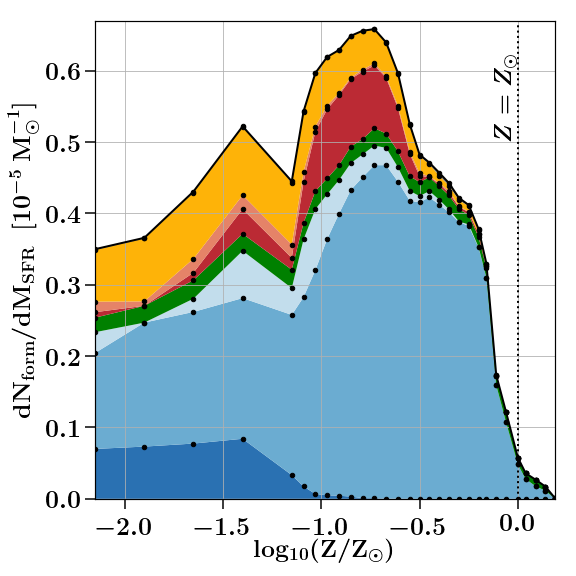
\includegraphics[width=\textwidth]{../PlottingScripts/3_DCO-Population/channelBHNS_pessimistic_small.png}
%%   \caption{Number of \bhnsSingle mergers per unit star forming mass  (\MSFR) for our grid of metallicities. Colours represent the different formation channels described in Section~\ref{subsec:bhns-BPS-formationChannels}. Black points denote the metallicities $\Zi$  that are  simulated. Lines between the simulation points show a linear interpolation between our models. }
%%   
%    \centering
%    \subfloat[]{{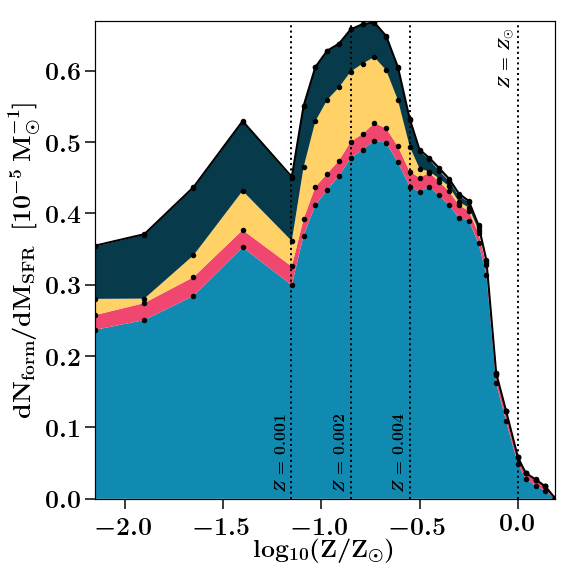
\includegraphics[width=1.0\columnwidth]{../PlottingScripts/3_DCO-Population/channelBHNS_pessimistic_small_4channels.png} }}%
%    \qquad
%    \subfloat[]{{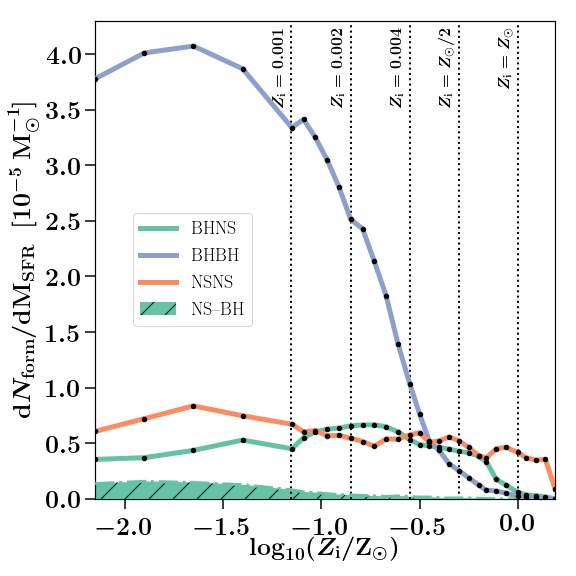
\includegraphics[width=1.0\columnwidth]{../PlottingScripts/3_DCO-Population/Rate_vs_Z_pessimistic_Fiducial.png} }}%
%      \qquad
%%    \caption{2 Figures side by side}%
%   \caption{Number of double compact object mergers with  delay times $\tdelay \leq \thubble$  that form per unit star forming mass  (\MSFR) per  metallicity $Z$ in our fiducial model for  {\sc{COMPAS}}.  \textbf{left:} only the \bhnsSingle rate with colours indicating the contribution of each formation channel (discussed in Section~\ref{subsec:bhns-BPS-formationChannels}, \textbf{right:} double compact object rates for BHNS (green) \ac{BHBH} (dark blue) and \ac{NSNS} (magenta) mergers. The green hashed area shows the subset of \bhnsSingle mergers where the \ac{NS} forms in the first SN.    \textbf{all:}  the 30 black scatter points denote the initial metallicities $\Zi$  that are  simulated. Lines between the simulation points show a linear interpolation between different metallicity outcomes. }
%  \label{fig:BHNS_rate_per_metallicity}
%\end{figure*}
%%
%
%
%The rate of \bhnsSingle systems that merge in a Hubble time per star-forming mass depends on the star formation metallicity. This is shown in the left panel of Figure~\ref{fig:BHNS_rate_per_metallicity}. 
%
%The general trend is that there are more mergers per unit star forming mass at lower metallicities, which is also found by  \citet[e.g.][]{2018MNRAS.481.1908K,2018MNRAS.480.2011G,2019MNRAS.490.3740N}. This is mostly a consequence from the line-driven stellar winds scaling positively with metallicity in our simulations (see Section~\ref{subsec:method-BPS-assumptions}):
%%
%
%First, at higher metallicities,  higher  wind-loss rates strip more mass from the star leading to stars with lower carbon-oxygen cores. These lower carbon-oxygen cores  result  in  lower compact object masses in the \citet{2012ApJ...749...91F} delayed  \ac{SN} remnant prescription in our \fiducial model. This leads both that  some  \bhnsSingle  systems instead  form  \ac{NSNS} systems at higher metallicities and to  lower  carbon-oxygen cores which are given  larger  \ac{SN} natal  kicks in our remnant mass prescription (see Section~\ref{subsec:method-BPS-SN-natal-kick-and-fallback}), which makes it more probable that the  \ac{SN}  disrupts the binary system lowering the number of \ac{GW} mergers. 
%Second, at higher metallicities, the stronger self-stripping through line-driven stellar winds  leads to stars losing more of their envelope mass. As a consequence a binary at higher metallicity typically has a lower total binary mass at the onset of the  \ac{SN} compared to lower metallicities. This makes the system more likely to disrupt during the  \ac{SN} as a consequence of the natal and Blaauw kick. 
%Finally, at higher metallicities,  binaries typically have wider separations after the second SN, which can also be seen from the bottom panels of Figure~\ref{fig:BHNS_DCOmasses}, and will therefore have longer inspiral time that may exceed the Hubble time. This is both because the stellar winds widen the binary and because they result in stars with less massive envelopes that reduces the amount of orbital hardening that typically happens during the mass transfer events (i.e., \ac{CE} and stable Roche-lobe overflow) in the evolution of the binary.  
%All the above effects cause the lower  \bhnsSingle merger rate  at higher metallicities in Figure~\ref{fig:BHNS_rate_per_metallicity}.
%At even lower metallicities, i.e., metallicities lower than about $1/10$-th solar, the \bhnsSingle rate decreases slightly as stellar winds are low enough that many carbon-oxygen cores stay massive enough to produce a \ac{BHBH} merger instead of a \bhnsSingle, as in agreement with findings by e.g.  \citet{2019MNRAS.482.5012C}. 
%
%
%In addition, the left panel in Fig~\ref{fig:BHNS_rate_per_metallicity} shows that formation channels other than the classic channel become only important at lower metallicities for \bhnsSingle mergers. 
%
%The right panel of  Figure~\ref{fig:BHNS_rate_per_metallicity} shows the rate of formation of \bhnsSingle systems that merge in a Hubble time in comparison with \ac{BHBH} and \ac{NSNS} mergers. It can be seen that 
%around solar metallicity the formation of \ac{NSNS} mergers dominates, whereas at metallicities $\log_{10}(Z/Z_{\odot}) \leq -0.5$ \ac{BHBH} mergers dominate the merger rate per unit star forming mass.  Interestingly, the BHNS and \ac{NSNS} formation rate are comparable for our fiducial model around metallicities lower than $\log_{10}(Z/Z_{\odot}) \leq -0.25$. 
%From this figure it is also apparent that among the double compact object types the \ac{BHBH} formation rate depends most strongly on metallicity, whereas the \ac{NSNS} and BHNS merger rate are more independent of metallicity. This is consistent with earlier findings by e.g. \citet[][]{2016MNRAS.462.3302E,2018MNRAS.480.2011G,2018MNRAS.474.2959G,2019MNRAS.482.5012C, 2019MNRAS.490.3740N}.
%
%It can also be seen from the right panel of Figure~\ref{fig:BHNS_rate_per_metallicity} that especially at lower metallicities there is a substantial fraction of \bhnsSingle mergers where the \ac{NS} forms in the first  \ac{SN} (i.e. a NS--BH merger). These systems origin from binaries that start initially with similar masses (i.e. $q \approx 1$, which only at lower metallicities form \bhnsSingle mergers (see also Figure~\ref{fig:BHNS_ZAMSmasses} and Section~\ref{subsec:bhns-BPS-ZAMSm1m2}).

%
%%\href{https://arxiv.org/pdf/1602.03790.pdf}{compare with this paper} compare with \citep{2016MNRAS.462.3302E}
%\href{https://arxiv.org/pdf/1811.03565.pdf}{and with this}


%
%\floor{The effects mentioned above don't change that much between low metallicities, and as a result the main effect is that the \bhnsSingle merger rate slightly decreases.}  \floor{I think this might be happening, but not sure..} 





%
%\begin{figure*}
%\includegraphics[width=\textwidth]{../PlottingScripts/3_DCO-Population/channelBHNS_pessimistic.png}
%   \caption{Number of \bhnsSingle mergers per unit star forming mass  (\MSFR) for our grid of metallicities. Colours represent the different formation channels described in Section~\ref{subsec:bhns-BPS-formationChannels}. Black points denote the metallicities $\Zi$  that are  simulated. Lines between the simulation points show a linear interpolation between our models. }
%  \label{fig:BHNS_rate_per_metallicity}
%\end{figure*}
%
%%
%\begin{figure}
%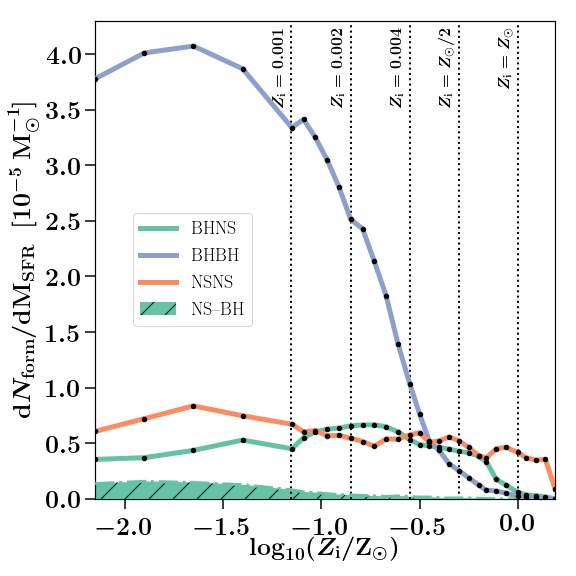
\includegraphics[width=\columnwidth]{../PlottingScripts/3_DCO-Population/Rate_vs_Z_pessimistic_Fiducial.png}
%   \caption{Number of \bhnsSingle mergers per unit star forming mass  (\MSFR) for our grid of metallicities. Colours represent the different formation channels described in Section~\ref{subsec:bhns-BPS-formationChannels}. Black points denote the metallicities $\Zi$  that are  simulated. Lines between the simulation points show a linear interpolation between our models. }
%  \label{fig:BHNS_rate_per_metallicity}
%\end{figure}
%%




%\subsection{\bhnsSingle characteristics  as a function of metallicity}
%\label{subsec:BHNS-mergerDistributions-asZ}
%
%\begin{figure*}
%\includegraphics[width=\textwidth]{../PlottingScripts/3_DCO-Population/CombinedZdistributions.png}
%   \caption{ Distributions of the characteristics of \bhnsSingle systems with \tmerger $\leq$ \thubble at the moment after the second  \ac{SN} for five different metallicities $\Zi$. From left to right and up to down:    the total mass $M_{\rm{tot}}$, mass ratio $q \equiv M_{\rm{BH}} / M_{\rm{NS}}$, chirp mass $\mathcal{M}_{\rm{c}}$, merger time $t_{\rm{merge}}$, \ac{BH} mass $ M_{\rm{BH}}$  and \ac{NS} mass $ M_{\rm{NS}}$. The yield is calculated using Equation~\ref{eq:formation-rate-COMPAS} (see also Appendix~\ref{sec:app-calculating-rate-BPS}) whereafter we plot the central points of the weighted histograms and connect these bin centers with a linear interpolation. The histogram binwidth is adapted to the number of \bhnsSingle and the range of the distribution.  }
%  \label{fig:BHNS_ObservableDistributions_per_metallicity}
%\end{figure*}
%%

%
%Figure~\ref{fig:BHNS_ObservableDistributions_per_metallicity} shows the histogram distributions of the \bhnsSingle characteristics for five different simulated metallicities $\Zi$  at the moment after the second  \ac{SN} and the binary has formed the \bhnsSingle system. 
%
%There are several trends in metallicity visible in the characteristics of the \bhnsSingle mergers.  First,  the yield (i.e. the area under the histogram) of \bhnsSingle mergers is highest around metallicities $Z= 0.001, Z=0.002$, which is also visible  in Figure~\ref{fig:BHNS_rate_per_metallicity} \todo{make these lines in Fig 5} and lowest at solar metallicity ($Z=0.0142$). 
%Second, at lower metallicities \bhnsSingle mergers are formed with more massive BHs compared to at higher metallicities, as can be seen in the plot of $M_{\rm{tot}}$,  ${M}_{\rm{BH}}$, $q$ and  $\mathcal{M}_{\rm{c}}$ that are more extended to higher masses for lower metallicities.  This is because at lower metallicities stars have less strong line-driven winds, and keep more of their envelope mass (see also Section~\ref{subsec:Metallicity-dependent-merger-rate-Rform}).
%
%
%There is a double peak in the  \ac{BH} masses, with one of the peaks  around the righter most edge of the distribution. This is because our LBV wind mass loss prescription maps a range of massive stars that enter the Humphreys-Davidson limit  to the same \ac{BH} remnant masses. This causes a sharp peak at the higher mass end in the \ac{BH} mass as also seen in (Fig 1 Belczynski 2010, Dominik 2012). 
%
%The neutron star mass, has a sharp peak at 1.3$\Msun$. This is because both US \ac{SN} and ECSN \ac{SN}  lead to low \ac{NS} remnant masses around $1.3\Msun$ see also section~\ref{subsec:method-BPS-ccSN}--\ref{subsec:method-BPS-ECSN}.
%
%%This causes a double peak behavior in the total mass and chirp mass and mass ratio. 
%%The mass ratio shows that most binaries have a more extreme mass ratio, caused by the \ac{BH} being more massive than the typical NS. However, in $X\%$ of the systems, the mass ratio is smaller than $1/3,( 1/5$) which are possible candidates to produce also  ejecta as the \ac{NS} is disrupted outside of the \ac{BH} innermost-stable-orbit. We find longer tails near equal mass ratios (compared to Figure9 Dominik 2012). This is both because our fiducial delayed prescription allows lower mass BHs, making it possible to have smaller mass ratios and because our large number of \bhnsSingle recovers more likely such tails of distributions. 
%







%The merger time
%
%peak in Mbh 
%peaks in Mns
%
%
%We find that $t_{\rm{merger}}$ can be as small as a few Myr as shown by (Dominik et al. 2012)
%
% $t_{\rm{merger}}$  distribution depends on metallicity. 
%
%\subsection{Delay times }
%\label{subsec:bhns-BPS-tdelay-distribution}
%%
% FROM SAFARZARDAH & BERGER 2019:
%After the formation of the BNS, the binary’s orbit decays through the emission of grav- itational waves on a timescale that depends on the bi- nary’s separation as t ∝ a4, where a is the semi-major axis of the binary at formation (Peters 1964). The dis- tribution of the merging times, therefore, depends on the distribution of the initial orbital separation modeled as dN /da ∝ a−β . The initial distribution of the O/B star (the progenitors of the NSs) is assumed to follow a power law dN/da ∝ a−1. If the binary goes through a common envelope phase, then the distribution of the separation becomes steeper and approaches dN/da ∝ a−3. There- fore, the expected merger times follow dN/dtmerge ∝ tΓ, where Γ ≡ −β/4 − 3/4. For those two limiting cases, Γ ranges from −1.5 to −1 (e.g., Belczynski et al. 2018).
%From population syn- thesis models tmin could be as short as a few Myr (Do- minik et al. 2012), but various effects could serve to set a minimum initial separation that will increase the value of tmin. Observationally,

%highly dependent on metallicity, the DTD for BNS sys- tems has been argued to be at most weakly dependent on metallicity (Dominik et al. 2012). The

%Recent simulations have shown that fast merging channels are needed to explain the fraction of all the metal-poor stars that are r-process enriched (Mat- teucci et al. 2014; Safarzadeh et al. 2018), as well as for r-process enrichment of ultra-faint dwarf galaxies (Sa- farzadeh & Scannapieco 2017; Safarzadeh et al. 2019).
%\subsection{eccentricity, neutron star mass, \ac{BH} mass, separation?}
%
%
%
%
%%
%%
%%
%\newpage
%
%\newpage
%
%\newpage
%
%\newpage
%

%

%\begin{figure*}
%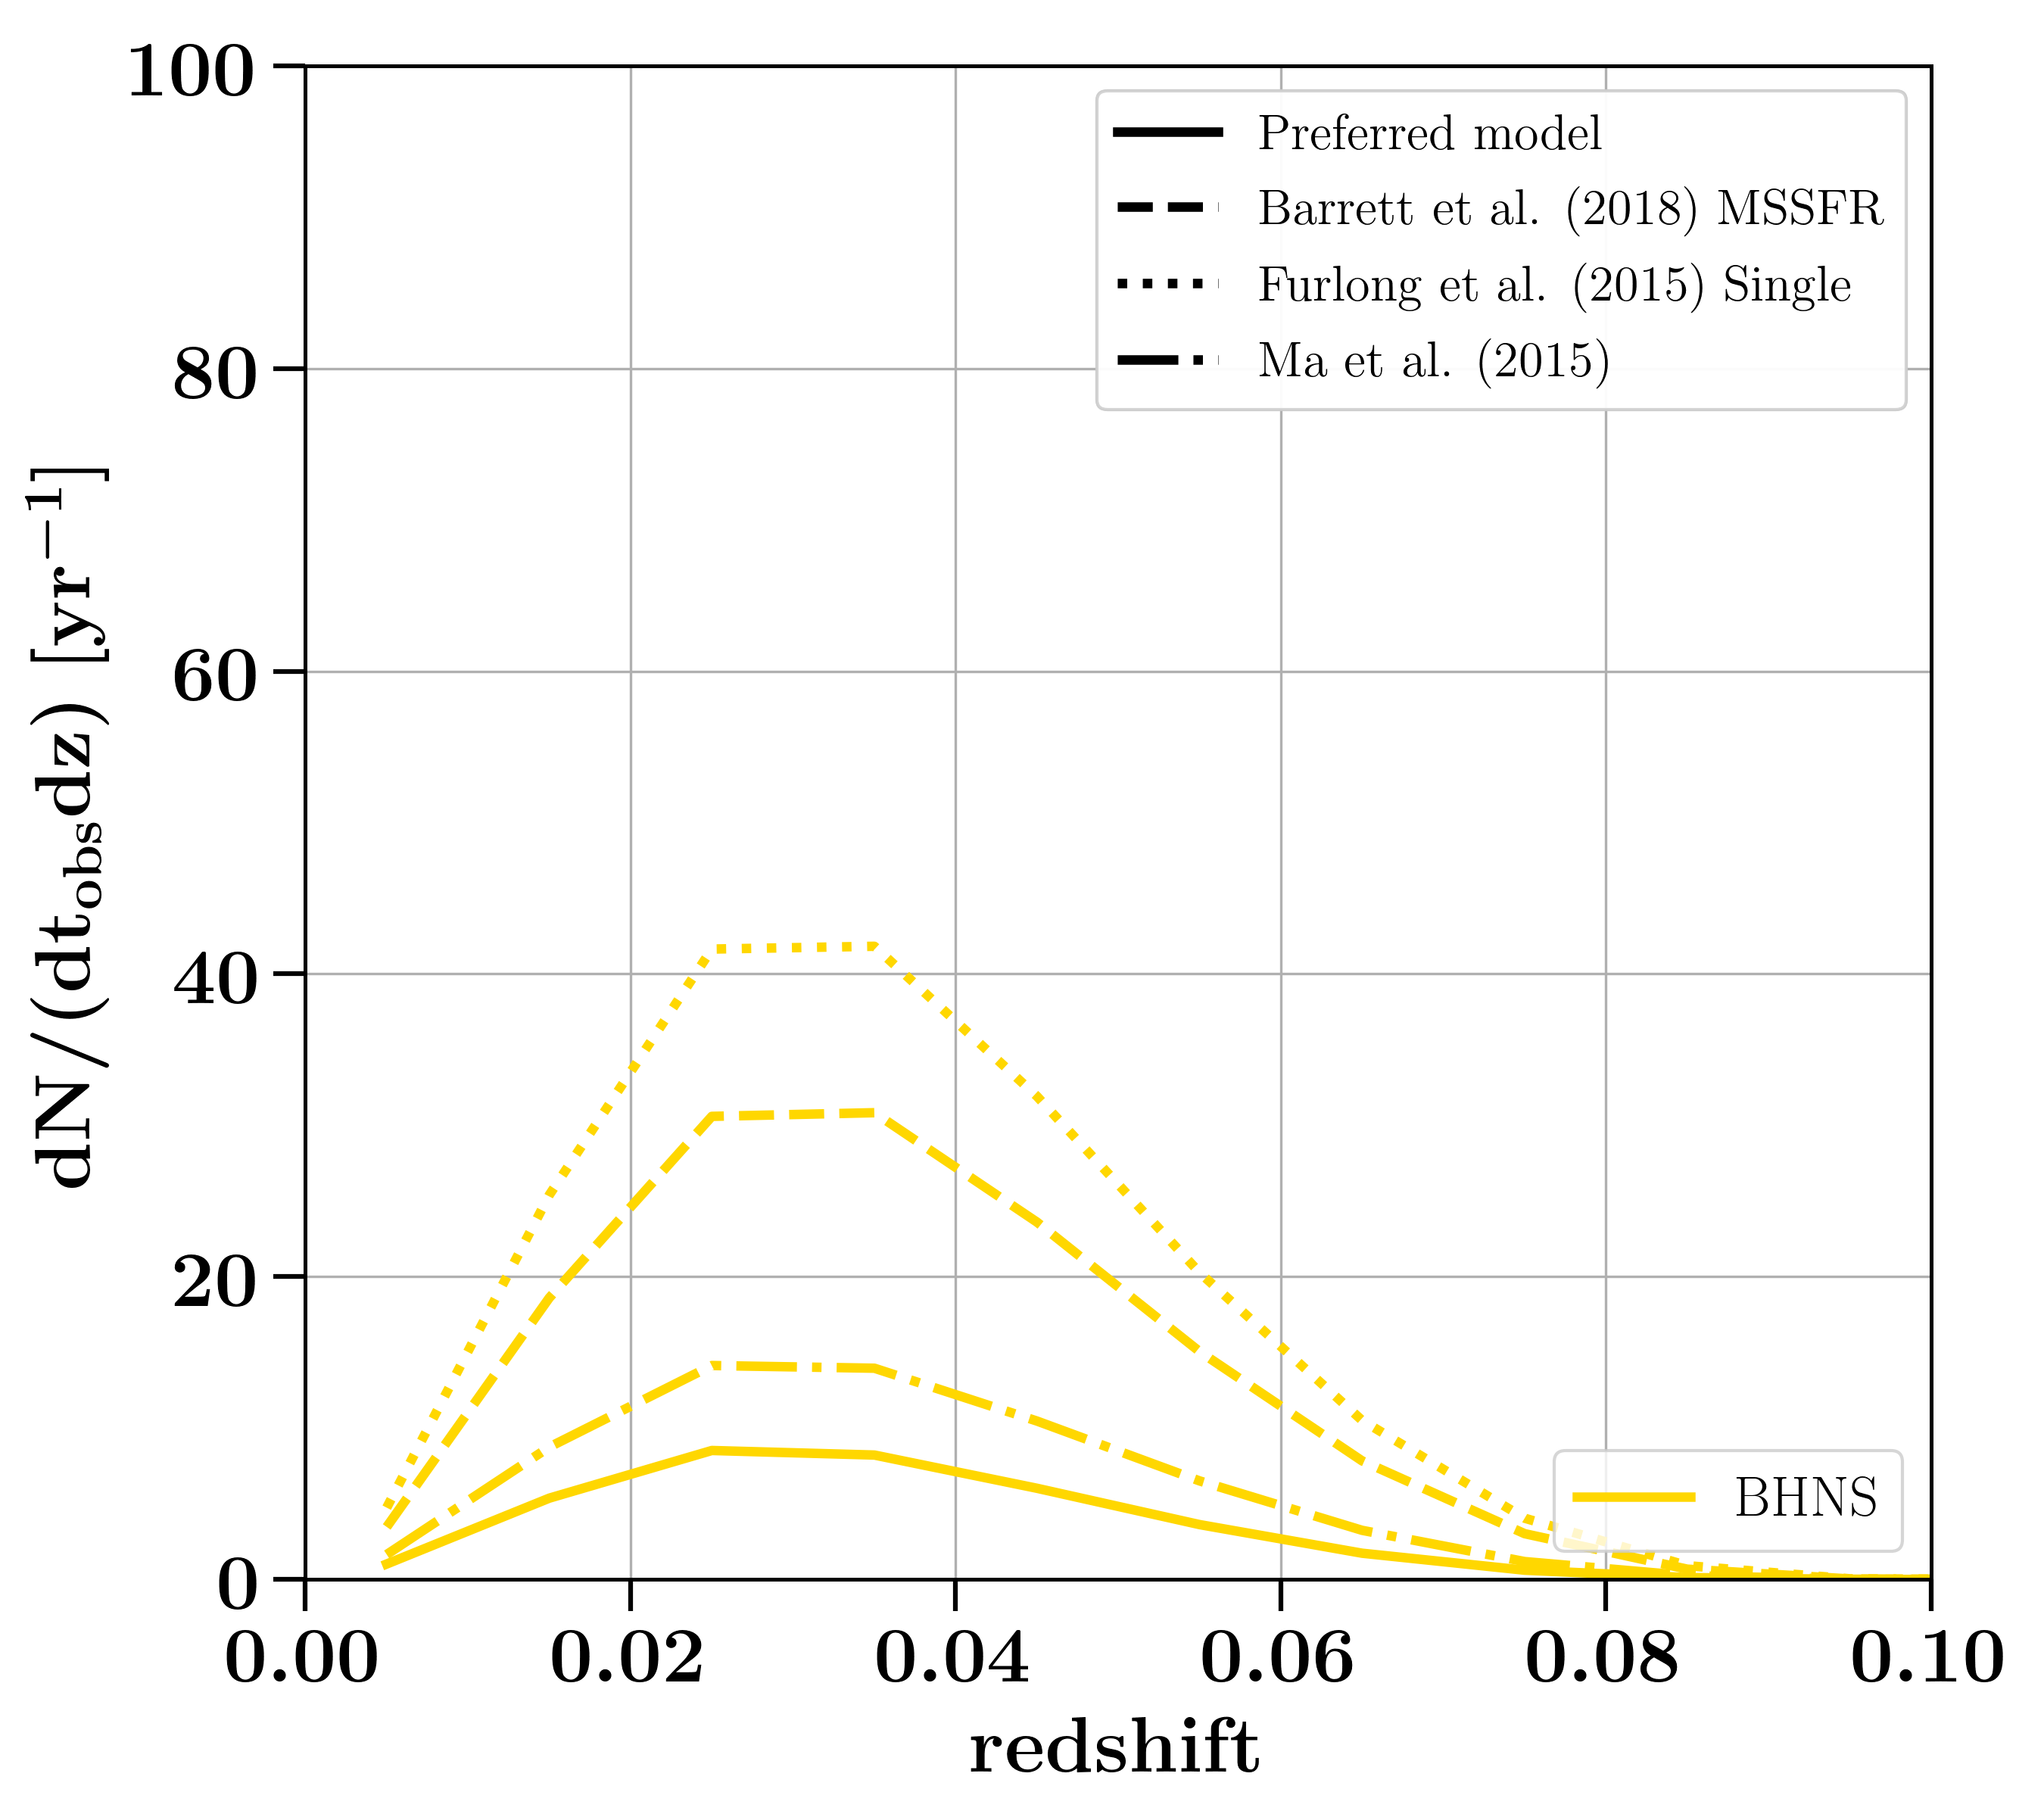
\includegraphics[width=\textwidth]{../PlottingScripts/4_MSSFR_observed/TotalMergerRateRedshiftObs-BHNS.png}
%   \caption{}
%  \label{fig:BHNS_DCO_c}
%\end{figure*}
%%
%



%
%\subsection{GW driven merger rates}
%
%
%\subsection{GW driven merger predictions}

%%
%\section{\ac{MSSFR} results fiducial simulation}
%\label{sec:bhns-MSSFR-fiducial}
%
%\href{https://arxiv.org/pdf/1811.03565.pdf}{compare with this}
%\subsection{BH--NS as a function of metallicity}
%





%%
%\begin{figure*}
%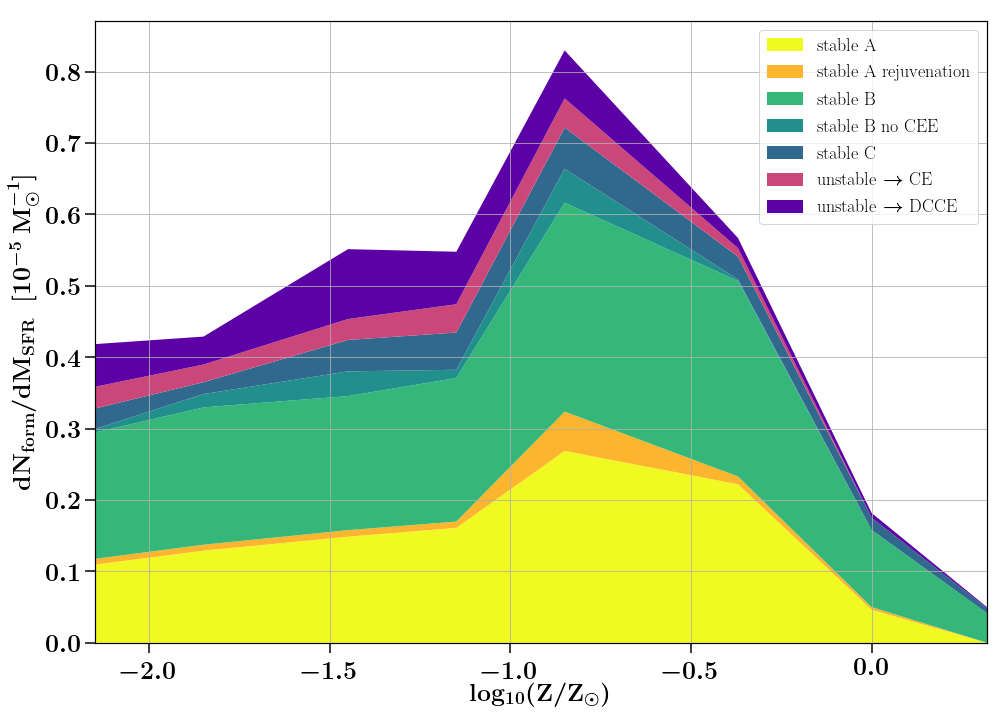
\includegraphics[width=.8\textwidth]{../PlottingScripts/3_DCO-Population/channelBHNS.png}
%   \caption{ }
%  \label{fig:BHNS_DCO_d}
%\end{figure*}
%
%The number of \bhnsSingle mergers is slightly  smaller at solar metallicity compared to lower metallicity. This is a result from (i) stronger stellar winds at higher metallicities that widens the binaries which increases the average time for a binary to merge.   And (ii) higher metallicities creating lower mass compact objects. These compact objects can less easily eject the \ac{CE} during a \ac{CE} event and therefore create less systems that survive this event. This leads to a slightly lower number of mergers. (iii) more massive compact remnants are more likely to survive the \ac{SN}  natal kick. 

%\begin{itemize}
%	\item GBH--NS rates change as function of metallicity
%	\item Also, distributions BH--NS change with Z, mostly \ac{BH} masses
%	\item 
%	\item assumptions for LIGO and Virgo O3
%	\item caveats
%	\item 
%\end{itemize}
%
%
%\section{BH--NS predictions for aLIGO}
%%
%


\subsection{Predicted GW observable \bhnsSingle distributions }
\label{subsec:distributions-FIducial-GW-observable}
%
%%% FIGURE : fiducial LIGO PREDICTIONS 




\begin{figure*}
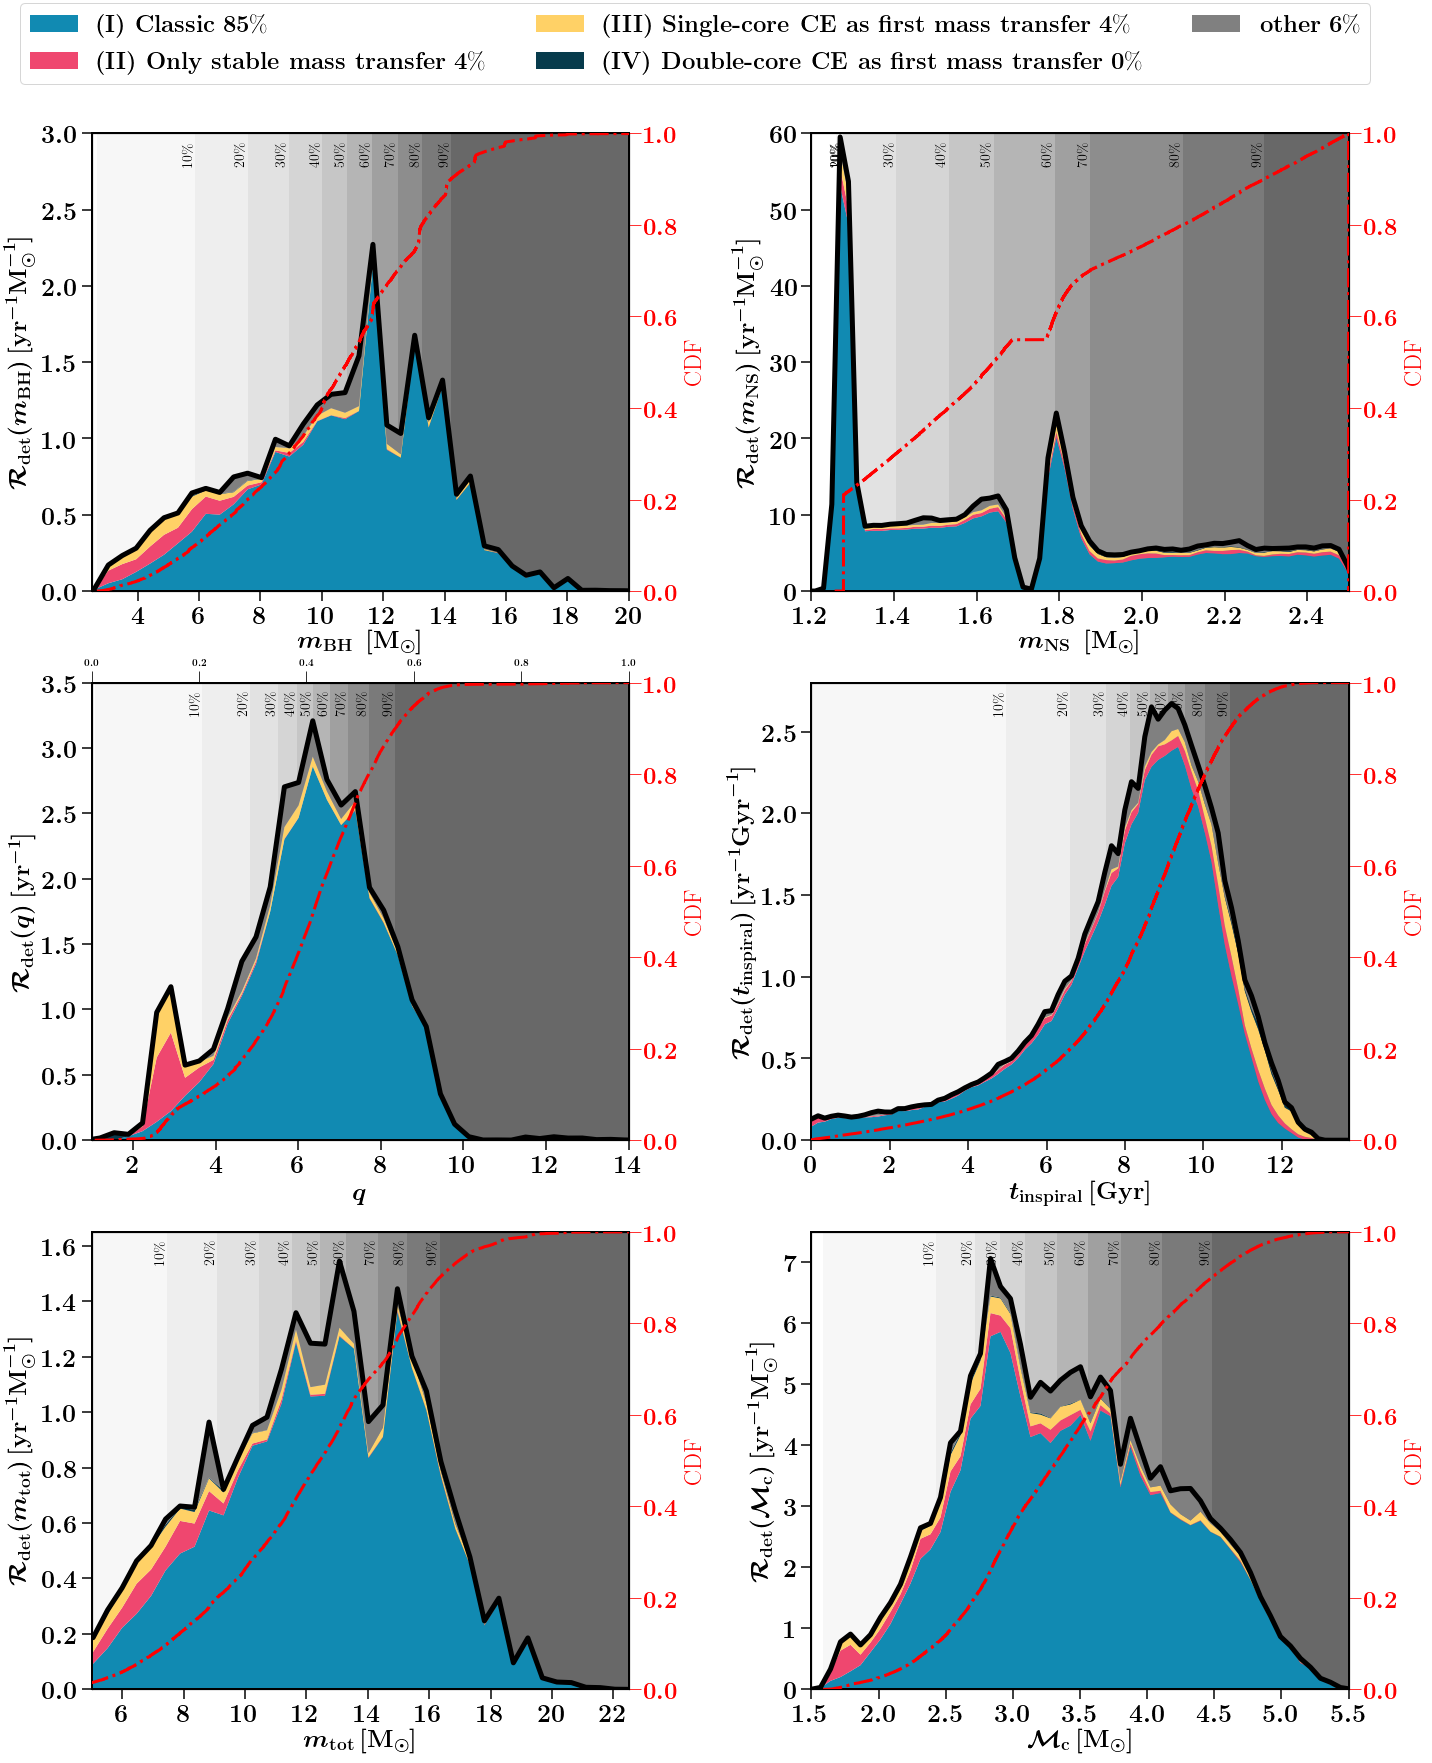
\includegraphics[width=.95\textwidth]{../PlottingScripts/7_Discussion/DistributionsFiducialchannels_observed_BHNS.pdf}
   \caption{ Predicted distributions of the  \bhnsSingle merger characteristics for our fiducial model for ground-based \ac{GW} detectors at design sensitivity.  From top to bottom and left to right we plot  \ac{BH} mass \mbhf, \ac{NS} mass \mnsf, mass ratio \qf = \mbhf / \mnsf,  inspiral time \tinspiral, total mass \mtotf and chirp mass \mchirpf. The yield is calculated using Equation~\ref{eq:rate_detector}. The colors in each graph, and the numbers quoted in the legend represent the percentage each formation channel contributes to the total observed yield presented in Section~\ref{subsec:bhns-BPS-formationChannels}.  The kde bandwidth factor are 0.25.  The gap in the \ac{NS} remnant mass distribution is caused by a discontinuity in the remnant mass prescription as discussed in Section~\ref{subsec:method-BPS-assumptions}. The red dashed-dotted lines show the cumulative distribution function (CDF). Gray areas indicate values for the CDF. }
  \label{fig:BHNS_DCO_observed}
\end{figure*}
%


The predicted distributions of \bhnsSingle characteristics as observed by the LVK \ac{GW} network at design sensitivity are shown in Figure~\ref{fig:BHNS_DCO_observed}. 
The distributions and yields are determined using Equation~\ref{eq:rate_detector}. These distributions are different from the \bhnsSingle distributions shown before as the detection probability \Pdet is added, taking into account that ground-based \ac{GW} detectors are  more sensitive to more massive systems and can only detect systems that merge in the horizon of the detector network.
The distributions for \ac{NSNS} and \ac{BHBH} mergers are given in Appendix~\ref{sec:app-fiducial-GW-predictions-for-BBH-BNS}. 


\subsubsection{Formation channels} 
Our fiducial model predicts that about  $90\%$ of the \bhnsSingle mergers  observed by the LVK network at design sensitivity forms through the classic formation channel (I) (see Section~\ref{subsubsec:classic-channel} and Figure~\ref{fig:formation-channels-sketch}). The classic formation channel produces relatively more massive \bhnsSingle systems, increasing the contribution of this channel to \ac{GW} observations. 
This  is different compared to the dominant channel for \ac{BHBH} and \ac{NSNS} mergers (see Appendix \ref{sec:app-fiducial-GW-predictions-for-BBH-BNS}).  For \acp{BHBH} $70\%$ of \ac{GW} detected  mergers are predicted to form through the only stable mass transfer channel (II)  \citep[c.f.][]{2019MNRAS.490.3740N}.  For \ac{NSNS} mergers about $60\%$ of the detected systems are predicted to form through the double-core \ac{CE} channel (IV).   
\bhnsSingle mergers are thus a good probe to study the formation of \ac{GW} sources that form through the classic formation channel compared to \ac{BHBH} and \ac{NSNS} mergers.  


\subsubsection{\ac{BH} mass} 
The fiducial model predicts that the \bhnsSingle mergers  will typically have $2.5 \leq \mbhf/ \Msun \leq 16$ with less than $5\%$ of observed \bhnsSingle mergers having $\mbhf >  15$\Msun (c.f.  \citealt[][]{2020arXiv200302277R}).  Progenitors for \bhnsSingle mergers with more massive \acp{BH}   typically lead to stellar mergers during the binary evolution.  
This is different for  \ac{BHBH} mergers where the majority of predicted \acp{BH} exceed  $15$\Msun (see Appendix~\ref{sec:app-fiducial-GW-predictions-for-BBH-BNS}). 


\subsubsection{\ac{NS} mass} 
 Our fiducial model predicts  a flat distribution in \ac{NS} mass with two peaks around $1.25$\Msun and 1.8\Msun. 
%The peaks are caused by the delayed remnant mass prescription and \todo{figure out peak 1.8\Msun} respectively. 
The \acp{NS} are  more massive compared to \ac{NSNS} mergers: about $ 70\% $ $(20\%)$ of the \bhnsSingle (NSNS) observations are predicted to have $\mnsf \geq 1.5$\Msun  \citep[c.f.][]{2018MNRAS.474.2959G}.
This mainly results from the \acp{NS} in  \bhnsSingle systems originating from more massive stars compared to \acp{NS} in \ac{NSNS} mergers. These more massive stars result in a more equal mass ratio stellar binary (since the binary also contains the  BH  progenitor), which is typically more likely to avoid a stellar merger and disruption during the \ac{SN}  in the binary evolution. 
Massive \acp{BH} in \bhnsSingle mergers typically have more massive \ac{NS} as can be seen in Figure~\ref{fig:BHNS_DCOmasses}, in agreement with e.g., \citet[][see Figure~7]{kruckow2018progenitors}.   
\bhnsSingle mergers are therefore important to study  \acp{NS} with \mnsf $> 1.5$\Msun. 



\subsubsection{Mass ratio} 
  The predicted \bhnsSingle merger mass ratios lie typically in the range $0.1 \leq \qf \leq 0.5$ where $\qf =\mnsf / \mbhf$ and peaks around  $\qf \approx 1/6$  (c.f. e.g. \citealt{2018MNRAS.474.2959G}) due to the typical \ac{BH} mass  around $\approx 13\Msun$. 
There is also a small second peak around $\qf \approx 1/3$ from contributions from channels II and IV (see Section~\ref{subsec:bhns-BPS-formationChannels}).  Compared to  \ac{BHBH} and \ac{NSNS} mergers where typically  more than 95$\%$ of the systems  have $\qf \leq 2$, \bhnsSingle mergers distinguish themselves by having more unequal compact object mass ratios (see Appendix~\ref{sec:app-fiducial-GW-predictions-for-BBH-BNS}). 


\subsubsection{Inspiral time} 
The \bhnsSingle inspiral times typically span \tinspiral $\sim [6,12]$\Gyrs.   
Although most \bhnsSingle that merge in a Hubble time are formed with   $\tinspiral \lesssim 2$\Gyr, the typical \ac{GW} observed system will have longer \tinspiral as a result from higher SFRs and  \bhnsSingle yields at higher redshifts (and longer lookback times).  
This is different compared to  \ac{NSNS} and \ac{BHBH} mergers that have inspiral times peaking at short inspiral times and a mixture of short and long inspiral times  (see Appendix~\ref{sec:app-fiducial-GW-predictions-for-BBH-BNS}). 
%This is because the inspiral time distribution is sensitive to the metallicity (and hence \ac{MSSFR} prescription) that the \ac{DCO} originate from (see for more details Section~\ref{subsec:results-MSSFR-MSSFR-variations}). 
The delay time distribution of these mergers can be constrained in the future from observations \citep{2019ApJ...878L..14S,2018ApJ...863L..41F} and might therefore help distinguishing \ac{MSSFR} and population synthesis models. 

\subsubsection{Total mass}
 The \bhnsSingle total masses lie in the range $5 \lessapprox \mtotf / \Msun \lessapprox 20$ and peak around \mtotf $\sim 15$\Msun. The total mass distribution follows the \mbhf distribution as the \ac{BH} mass dominates the total mass for \bhnsSingle mergers. 

\subsubsection{Chirp mass}
The predicted chirp masses of the  \bhnsSingle mergers lie in the range $1.5 \lessapprox \mchirpf/ \Msun \lessapprox  5.5$ with a broad peak around $\sim3.5$\Msun. 


Less than 10$\%$ of the \bhnsSingle systems have total masses or chirp masses that overlap with the distribution of total masses for \ac{NSNS} or \ac{BHBH} mergers. Together with the sharp boundaries between the \bhnsSingle versus \ac{NSNS} and \ac{BHBH} in the mass ratios and individual masses this information could make it possible to distinguish the different \ac{DCO} types from \ac{GW} observations \citep[c.f.][]{2013ApJ...766L..14H,2015ApJ...807L..24L,2015MNRAS.450L..85M,2018ApJ...856..110Y} even for our fiducial model that does not  assume a lower \ac{BH} remnant mass gap.





\subsection{\ac{NS} disruption} 
we predict that in $\sim [2\%, 6\%, 13\%, 24\% ]$ of the \bhnsSingle mergers detectable with ground-based \ac{GW} observatories at design sensitivity the \ac{NS} will be disrupted outside the \ac{BH} and can potentially have an electromagnetic counterpart. These percentages are given for when assuming respectively a \ac{NS} radius and fixed spin for all \acp{BH} of: $(R_{\rm{NS}}, \chibh) = [(11.5\km,0), (13\km,0), (11.5\km, 0), (13\km, 0.5)]$. For a given model, the highest fractions of \bhnsSingle mergers with nonzero ejecta mass is for systems with large \ac{NS} radii and large BH spins, where especially the spins of the \ac{BH} are dominant.  Even in the more pessimistic scenario we still expect $2\%$ of the observed \bhnsSingle mergers to disrupt the \ac{NS} outside the \ac{BH} inner-most-stable-orbit. 








\section{Varying model assumptions}
\label{sec:results-variations}
%



%%
\begin{figure*}
    \centering
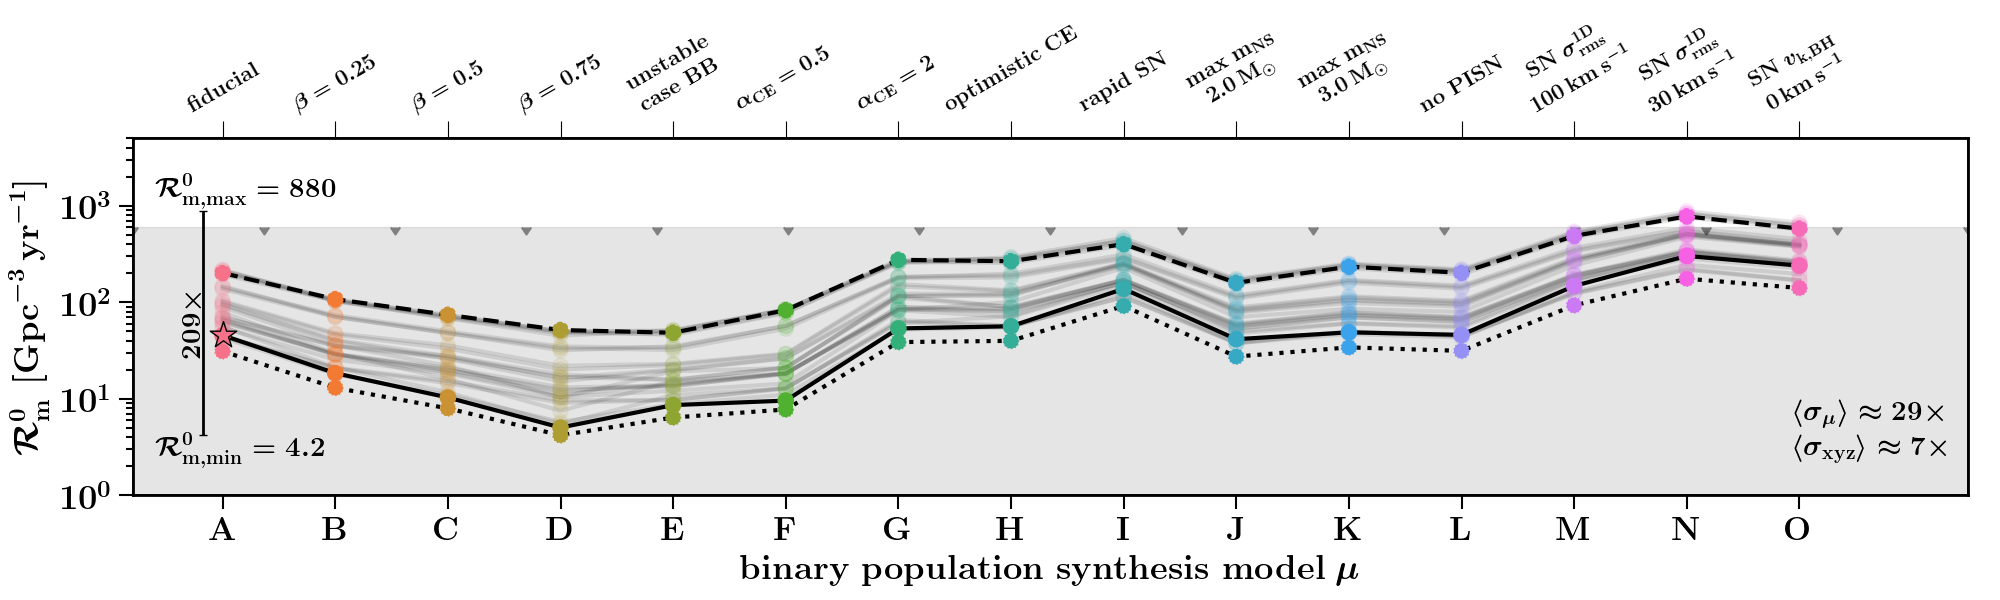
\includegraphics[width=1.0\textwidth]{../PlottingScripts/8_PredictedRates_BPS_and_MSSFR_variations/Rates_intrinsic_BHNS_Colors.png} %
    \caption{Predicted intrinsic rates for BHNS mergers  for different population synthesis and MSSFR models.  
    The rates are for mergers at $z=0$ without applying \ac{GW} selection effects. 
    We show for each of the \NmodelsBPS binary population synthesis model variation (given in Table~\ref{tab:variations-BPS}) the \bhnsSingle merger rates for the \NmodelsMSSFR variations in \ac{MSSFR} (given in Table~\ref{tab-MSSFR-variations-labels}). 
    Three \ac{MSSFR} variations: \rm{xyz}$=$000 (solid), 231 (dashed) and 312 (dotted)  are highlighted,  corresponding to our fiducial \ac{MSSFR} model and the models resulting in one of the highest and lowest rate predictions. The gray area shows the $90\%$ confidence interval for the observed \bhnsSingle rate  upper limit from  \citep{2019PhRvX...9c1040A}. Our fiducial model  (\mAzero) estimate is shown with a star symbol. On the right of the  panel  $\langle \sigma_{\mu}\rangle$ and $\langle \sigma_{\rm{xyz}}\rangle$ represent the mean scatter  in  rates caused over binary population synthesis and \ac{MSSFR} variations respectively. The minimum and maximum rates and the ratio between those are quoted on the left.  We use the short-hand notation $\rate_{\rm{m}}^0 \equiv (\diff \Ndet^2 / \diff \ts \diff \Vc)(\tmerger(z=0))$. }%
    \label{fig:IntrinsicRates}
\end{figure*}
%


%
\begin{figure*}
    \centering
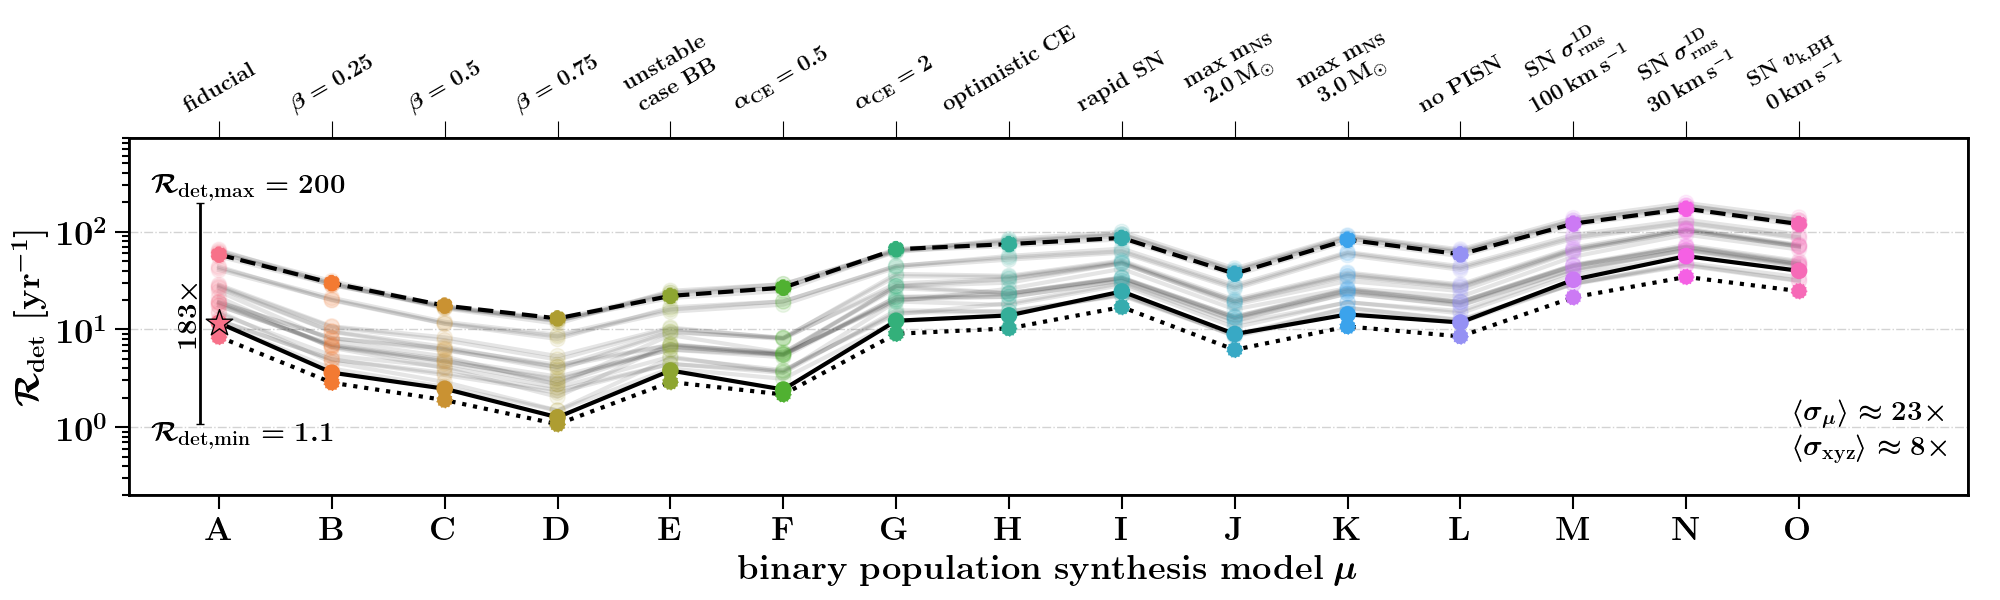
\includegraphics[width=1.0\textwidth]{../PlottingScripts/8_PredictedRates_BPS_and_MSSFR_variations/Rates_observed_BHNS_Colors.png} %
%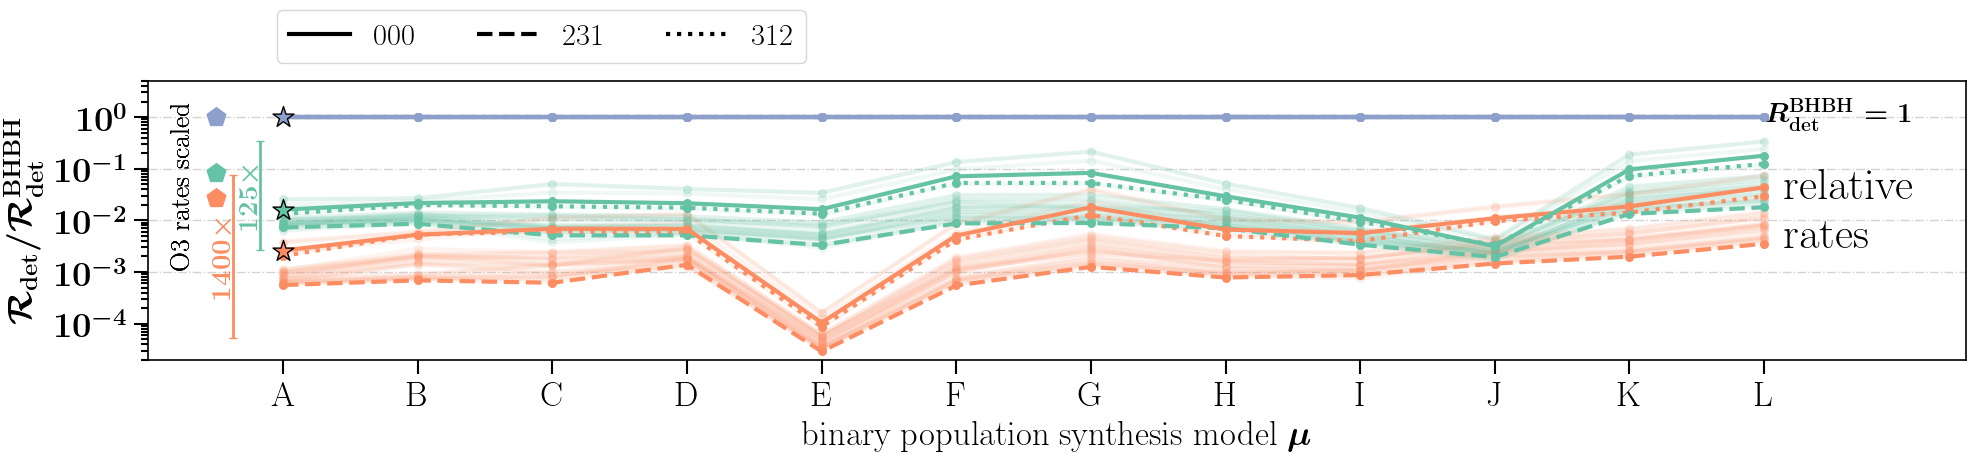
\includegraphics[width=1.0\textwidth]{../PlottingScripts/8_PredictedRates_BPS_and_MSSFR_variations/RatesRatios_observed.png} 
    \caption{Same as Figure~\ref{fig:IntrinsicRates} but for the predicted  detectable rates for a \ac{GW} network at design sensitivity. We use the short-hand notation $\rate_{\rm{det}} \equiv \diff \Ndet / \diff \tdet$.}%
    \label{fig:ObservedRates}
\end{figure*}
%


The predicted rates and characteristics of  \bhnsSingle mergers are sensitive to uncertainties in binary population synthesis and \ac{MSSFR}  model assumptions. 
After presenting the predictions for our fiducial model  \mAzero in Section~\ref{sec:results-fiducial} we compare in this section the predicted \bhnsSingle merger rates and characteristics for a total of \Nmodels  combinations of the \NmodelsBPS binary population synthesis and  \NmodelsMSSFR \ac{MSSFR} models. 
These model variations are summarized in Table~\ref{tab:variations-BPS} and~\ref{tab-MSSFR-variations-labels} respectively.  







\subsection{Intrinsic \bhnsSingle merger rates}
\label{subsec:results-variations-rates}
%
The predicted intrinsic rates for \bhnsSingle mergers are shown for different combinations of binary population synthesis and \ac{MSSFR} models in Figure~\ref{fig:IntrinsicRates}. 
These rates are calculated using Equation~\ref{eq:MSSFR-merger-rate}  and do not yet take into account the \ac{GW} selection effects.  
We find that the intrinsic \bhnsSingle merger rates are predicted to lie in the range $\rate_{\rm{m}}^0 \sim$ [\RateIntrinsicAzeroBHNSmin, \RateIntrinsicAzeroBHNSmax]  \GpcminThree \yearmin  and that our fiducial model predicts $\RateIntrinsicZero \approx \RateIntrinsicAzeroBHNS $\GpcminThree \yearmin.

Most of the predicted rates in Figure~\ref{fig:IntrinsicRates} are consistent with the observed $90\%$ confidence interval  for the \bhnsSingle merger rate upper limit from the first two \ac{GW} observing runs from \citet{2019PhRvX...9c1040A}. 
The exceptions are  the binary population synthesis models {G} (no BH kicks) and {L}  (low SN kicks) where some of the higher yield \ac{MSSFR} models  over-predict the upper limit for the observed intrinsic \bhnsSingle merger rate. 
In Section~\ref{sec:comparing-with-BHBH-and-NSNS} we show that these models also over-predict the observed intrinsic \ac{BHBH} merger rate although they are favored to match the observed intrinsic \ac{NSNS} rate. 



\subsection{GW detected \bhnsSingle merger rates}
\label{subsec:results-variations-rates-observed}
%
The predicted detected  rates for  \bhnsSingle  mergers  are shown in Figure~\ref{fig:ObservedRates}. 
These rates are calculated using Equation~\ref{eq:rate_detector} for a ground-based \ac{GW} detector network at design sensitivity. 
Our fiducial model predicts $\rate_{\rm{det}}  \sim \rateObsBHNS  \yearmin.$ Considering the \Nmodels model variations we find predicted  rates in the range $\rate_{\rm{det}} \sim [\RateObservedAzeroBHNSmin, \RateObservedAzeroBHNSmax]\yearmin$. 


\subsection{Fraction of \bhnsSingle mergers with possible electromagnetic counterparts}
\label{subsec:fraction-BHNS-with-EM-ejecta}
%
Figure~\ref{fig:ObservedRatesNSdisrupted} shows our predictions for the fraction of detected \bhnsSingle mergers for which the \ac{NS} is disrupted outside the \ac{BH}. We find that the fractions span the range $[0, 0.57]$.  
% innermost-stable-orbit which are potential sources to have a detectable counterpart to their \ac{GW} observation. If this is the case the ejected mass is nonzero.  
 The rapid \ac{SN} remnant mass prescription model (F)  gives the lowest fraction where for the 11.5\km \ac{NS} radius and zero \ac{BH} spin assumption no systems disrupt the \ac{NS} outside of the \ac{BH}. This is because model F  does not produce, by construction,  any \acp{BH}  with masses  $ \mbhf \lesssim6$\Msun which are the  \ac{BH} masses that can disrupt the \ac{NS} outside of the \ac{BH}  for the most pessimistic \ac{NS} radius and \ac{BH} spin assumption.  At the same time, model F also predicts the highest fraction of \ac{NS} disruptions as high as $\approx 0.57$ as this model has a relatively low fraction
of \bhnsSingle mergers with very massive \acp{BH} where the \ac{NS} always plunges in.


\subsection{BH--NS and NS--BH merger rates}
\label{subsec:fraction-BHNS-with-NSBH}
%


\bhnsSingle systems where the \ac{NS} forms first are interesting as the first formed \ac{NS} can spin up during mass transfer episodes and eventually form a millisecond-pulsar-\ac{BH} binary that is observable with radio telescopes. 
Detecting  such a system would provide a unique laboratory to test general relativity and alternative theories of gravity \citep{Wex:1998wt,KRAMER2004993, 2014arXiv1402.5594W} and will enable high precision  measurements of the  properties of black holes    \citep{1975ApJ...198L..27B,1975SvAL....1....2B}. However, to date, no pulsar--BH system has been observed through radio observations. This might not entirely be surprising as several studies estimate that the fraction of   pulsar--\ac{BH}  over \ac{NSNS} in our Milky Way is about $1/1000$ \citep{2005ApJ...628..343P}. Currently there are about 20 \ac{NSNS} known \citep[e.g.][]{tauris2017formation,2019ApJ...876...18F}. 


Figure~\ref{fig:ObservedRatesNSBH} shows for our \Nmodels model variations the fraction of \bhnsSingle mergers where the \ac{NS} formed first (NS--BH systems).  We predict fractions of NS--BH mergers  in  the range $[0.0011, 0.28]$. 
The highest fraction of NS--BH mergers is in the optimistic-\ac{CE} model (B). This is because most NS--BH systems form from binaries where the first mass transfer occurs relatively early on (case A or early case B mass transfer). In our model this phase of mass transfer is typically highly conservative and the stars can therefore exchange a large fraction of mass and reverse in masses, making the initial primary star the least massive star in the system and eventually form the \ac{NS}. Such systems also typically undergo a \ac{CE} phase initiated by a donor star on the Herzsprun gap, which are assumed to lead to a stellar merger in the pessimistic \ac{CE} models. An example of the evolution of such a binary is given in Appendix~\ref{app-example-of-evolution-NS-BH-system}. Such NS--BH systems might be distinguishable in \ac{GW} observations by measuring a high $\chi_{\rm{eff}}$ for the \ac{NS}. 

In addition,  NS--BH systems are thought to make up the majority of detectable pulsar-BH systems (compared to BH--NS systems) \citep{2020MNRAS.494.1587C}. In Appendix~\ref{sec:app-predicted-rates-intrinsic} we show that the fraction of NS--BH systems is similar for the intrinsic \bhnsSingle rates as compared to the \ac{GW} detectable rates. Detections of pulsar-BH systems through radio surveys can therefore add to the picture and help constrain  binary population synthesis models.   More detail is studied in future work.



%
\begin{figure*}
    \centering
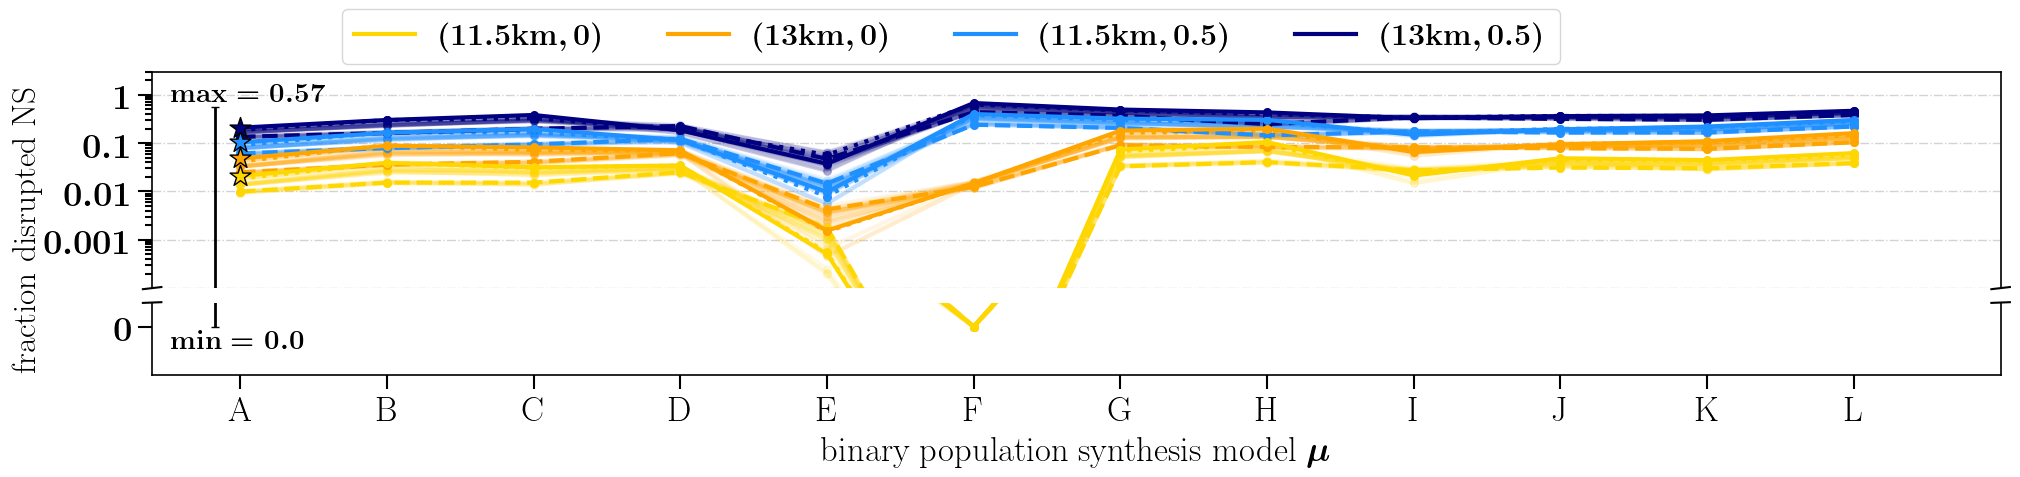
\includegraphics[width=1.0\textwidth]{../PlottingScripts/8_PredictedRates_BPS_and_MSSFR_variations/EMRatios_observedlog.png} 
    \caption{Same as Figure~\ref{fig:IntrinsicRates} but now showing the fraction of \ac{GW} detected \bhnsSingle mergers that disrupts the \ac{NS} outside of the \ac{BH}. Different colors show our different set of assumptions for the \ac{NS} radii and \ac{BH} spins.  }
%    observed rates that are obtained by taking into account the \ac{GW} selection effects (Section~\ref{subsec:detection-probability}). The percentage quoted on the y-axis is given by the ratio $\rate_{\rm{det}}^{\rm{NS--BH}}   / (100 \rate_{\rm{det}}^{\rm{NS--BH}})$}%
    \label{fig:ObservedRatesNSdisrupted}
\end{figure*}
%

%
\begin{figure*}
    \centering
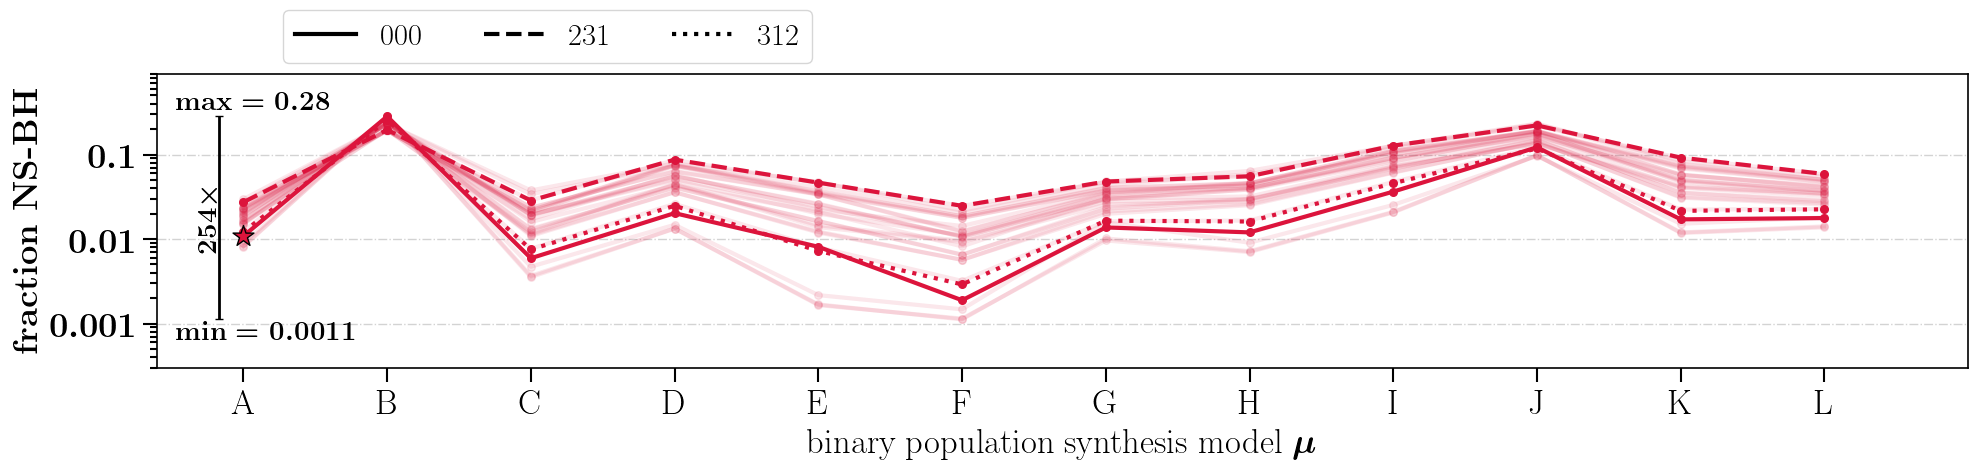
\includegraphics[width=1.0\textwidth]{../PlottingScripts/8_PredictedRates_BPS_and_MSSFR_variations/NSBHRatios_observedpercentage.png} 
    \caption{Same as Figure~\ref{fig:IntrinsicRates} but now showing the fraction of \ac{GW} detected \bhnsSingle mergers where the \ac{NS} forms first. } 
%    $\rate_{\rm{det}}^{\rm{NS--BH}}   / (100 \rate_{\rm{det}}^{\rm{BHNS}})$, where we fixed the total \bhnsSingle merger rate \bhnsSingle = BH--NS $+ $ NS--BH $=100$.}%
    \label{fig:ObservedRatesNSBH}
\end{figure*}
%



\subsection{Effect of varying binary population synthesis and \ac{MSSFR} assumptions  on the predicted  \bhnsSingle rates}
%
To quantify the scatter in the predicted rates  we calculate  the mean of the ratios between the maximum and minimum predicted rates given by
%
\begin{equation}
\langle \sigma_{\rm{\mu}} \rangle = \frac{1}{12} \sum_{\mu=A}^{\mu=L}
 \frac{\rm{max}(\rate_{\rm{m, \mu000}}^0,... ,\rate_{\rm{m, \mu333}}^0 )}{\rm{min}(\rate_{\rm{m, \mu000}}^0,... ,\rate_{\rm{m, \mu333}}^0 ) }, 
\end{equation} 
%

and 
%
\begin{equation}
\langle \sigma_{\rm{xyz}}\rangle = \frac{1}{28} \sum_{\rm{xyz}=000}^{\rm{xyz}=333}
 \frac{\rm{max}(\rate_{\rm{m, Axyz}}^0,... ,\rate_{\rm{m, Lxyz}}^0 )}{\rm{min}(\rate_{\rm{m, Axyz}}^0,... ,\rate_{\rm{m, Lxyz}}^0)}.
\end{equation} 
%

%
The  values for the scatter caused by binary population synthesis and \ac{MSSFR} uncertainties are quoted for our \bhnsSingle mergers   in  Figure~\ref{fig:IntrinsicRates} and \ref{fig:ObservedRates}.  
We find that for both the predicted intrinsic and detected \bhnsSingle merger rates  $\langle \sigma_{\rm{\mu}}\rangle \approx 30$ and $\langle \sigma_{\rm{xyz}}\rangle  \approx 10$. This means that variations from binary population synthesis assumptions  dominate the uncertainty in the predicted rates compared to \ac{MSSFR} variations for \bhnsSingle mergers.  We also find that the uncertainties in binary population synthesis and \ac{MSSFR} are somewhat independent:  the variation on the rates from \ac{MSSFR} uncertainty is typically $\approx 10$ for  any given binary population synthesis model and vice versa. 


%The variations in binary population synthesis models result in 
%average scatter in the predicted \bhnsSingle rates of $\langle \sigma_{\rm{\mu}}\rangle \approx 89\times$ and  $\langle \sigma_{\rm{\mu}}\rangle  \approx 80\times$ and scatter from \ac{MSSFR} of  $\langle \sigma_{\rm{xyz}}\rangle  \approx 8\times $ and $\langle \sigma_{\rm{xyz}}\rangle  \approx 9\times$ for intrinsic rates and detected rates respectively. 




%In total we see variations in the predicted detectable merger rates of factors $\sim 93\times, 123\times, 212\times$ for BHBH, \bhnsSingle and \ac{NSNS} mergers respectively. 


\subsubsection{Effect from binary population synthesis variations}


 The highest predicted \bhnsSingle rates are found in the binary population synthesis models A, B, F, G, K and L, which typically predict $\RateObserved \gtrsim 10$\yearmin.    The optimistic \ac{CE} model (B) is the variation on our fiducial model  where we allow Hertzsprung gap donors that engage in a \ac{CE} event to survive.  In this model the \bhnsSingle merger rate is therefore enhanced compared to the fiducial model as a significant number of \bhnsSingle systems forms through a \ac{CE} with a Hertzsprung gap donor. Figure~\ref{fig:ObservedRatesNSBH} shows that model B is especially important for forming a large fraction of NS--BH systems. Models  G, K and L all have lower \ac{BH} and/or \ac{NS} natal kicks compared to our fiducial model, which increases the fraction of systems that stay bound during the \acp{SN} and therefore increases the \bhnsSingle merger rate compared to our fiducial model. 
  
%In appendix \ref{sec:app-predicted-rates} we show that models G, K and L also increase the \ac{NSNS} merger rates whilst the   \ac{BHBH} rates stay similar. These models therefore  increase the ratio of \bhnsSingle and \ac{NSNS} mergers over \ac{BHBH} mergers.    Model F (rapid remnant mass prescription), on the other hand has slightly higher SN kick magnitudes which leads to more systems being disrupted and a slightly lower \bhnsSingle merger rate compared to the fiducial model as can be seen in Figure~\ref{fig:IntrinsicRatesApp_GSMF} and \ref{fig:ObservedRates}. 
%  
% 
Models H, I and J show that when we change  the mass transfer efficiency  to respectively $0.25, 0.5 $ and $0.75$ that this leads to a decreasing \bhnsSingle rate.  This seems counter-intuitive since higher values for $\beta$ correspond to more mass accretion by a star during mass transfer, which intuitively leads to the formation of more \acp{BH} and higher \bhnsSingle merger rates. However, there is another effect: the detectable  systems are highly biased towards tight binaries that merge within a Hubble time. As almost all our \bhnsSingle mergers go through a \ac{CE} phase, the more massive companion leads to a more massive shared envelope  that needs to be successfully ejected to avoid a stellar merger from the \ac{CE} event. This leads to  fewer \bhnsSingle systems as in agreement with findings by e.g.  \citet{kruckow2018progenitors}.  Figure~\ref{fig:ObservedRatesNSBH} shows that the fraction of  NS--BH mergers, on the other hand, increases for increasing $\beta$. This is because in this case the contribution of systems that merge as a result from a failed  \ac{CE} ejection is relatively low as these binaries form from typically initially lower mass stars and  will typically have a lower mass envelope in the \ac{CE} compared to BH--NS binaries. 

% model F has slightly larger kicks, thats why it reduces the kick slightly

%This is different for the \bhnsSingle and \ac{NSNS} rates where the scatter in predicted rates in our model variations is largest by the binary population synthesis assumptions. Especially for \ac{NSNS} mergers the model variations dominate. The \ac{MSSFR}  only makes the predicted \ac{NSNS} rates vary by a factor $\sim 5\times$ which is mostly because the formation yield of \ac{NSNS} is not as sensitive to metallicity compared with \ac{BHBH} (see Figure~\ref{fig:BHNS_rate_per_metallicity}). 
%
%For \bhnsSingle mergers, especially models C, D, E and J lead to low merger rates. For \ac{NSNS} mergers this is model E. \floor{interpertate this}
%
%We find that the predicted rates can vary factors of $\sim 48\times $, $109\times $ and $292\times $ for \ac{BHBH} \bhnsSingle and \ac{NSNS} respectively. 
%Future constrains from \ac{GW} observations on the predicted rates will help constrain between binary population synthesis and \ac{MSSFR} variations. Where \ac{BHBH} will especially be good probes to study \ac{MSSFR} and \bhnsSingle and \ac{NSNS} are probes for model variations. 


\subsubsection{Effect from \ac{MSSFR} variations  }
\label{subsec:effect-from-MSSFR-variations}

For a given binary population synthesis model, the highest predicted \bhnsSingle rates are from the \ac{MSSFR} models with the  \citet{2006ApJ...638L..63L}   \ac{MZR} (the models $\rm{xy}1$). For a fixed galaxy mass, this   \ac{MZR} relation results in lower star formation metallicities compared to the other \ac{MZR}  variations (see Appendix A of  \citealt{2019MNRAS.490.3740N} for more details). 
This leads to a higher fraction  of stars that form \acp{BH} and therefore to a higher yield of \bhnsSingle mergers. 
The other two MZR,    \citet{2006ApJ...638L..63L} $+$ offset and \citet{2016MNRAS.456.2140M}, corresponding to $\rm{xy}2$ and $\rm{xy}3$ respectively,   lead to lower \bhnsSingle  yields.  
We find that the \ac{MZR} dominates the uncertainty in the predicted rates, consistent with findings by e.g.  \citet{2019MNRAS.487.1675A, 2019MNRAS.488.5300C}.

For the \ac{SFR}  we find that the  \citet{2004ApJ...613..200S} \ac{SFR}  ($2\rm{yz}$)  typically has the highest yields, followed by the {\citet{2014ARA&A..52..415M}}  ($1\rm{yz}$) and  \citet{2017ApJ...840...39M}  ($3\rm{yz}$) \ac{SFR}  assumptions. 

For the GSMFs we find the highest yield is given by the  \citet{2015MNRAS.450.4486F} functions, either single or double Schechter,  which both give almost identical yields. 
On the other hand, the \citet{2004MNRAS.355..764P}  \ac{GSMF}  ($\rm{x}1\rm{z}$) leads to  relatively lower \bhnsSingle merger  yields. 

In total this leads to the \ac{MSSFR} models   $\rm{xyz}=231$ and $\rm{xyz}=312$  having (one of)  the highest and lowest \bhnsSingle merger yields for each binary population synthesis model,    as can be seen in Figures~\ref{fig:IntrinsicRates} and \ref{fig:ObservedRates}. Our fiducial \ac{MSSFR} model (000) also produces one of the lowest yields.   More details are presented in the figures in Appendix~\ref{sec:app-predicted-rates-MSSFR}.


%%% OLD PARAGRAPH
%
%The predicted intrinsic rates for BHBH, \bhnsSingle and \ac{NSNS} mergers are shown for different combinations of binary population synthesis and \ac{MSSFR} models in Figure~\ref{fig:IntrinsicRates}. 
%These rates are calculated using Equation~\ref{eq:MSSFR-merger-rate}  at redshift zero and do not yet take into account the \ac{GW} selection effects.  
% The intrinsic merger rates are in the ranges $\rate_{\rm{m}}^0 \sim$ [15, 740], [2.5, 1410] and [0.6,  440] \GpcminThree \yearmin for BHBH, \bhnsSingle and \ac{NSNS} mergers respectively. 
% 
%Most of the predicted rates in Figure~\ref{fig:IntrinsicRates} are consistent with the observed $90\%$ confidence interval of the rates from \citep{2019PhRvX...9c1040A,2020arXiv200101761T} with two exceptions.
%First, a subset of the \ac{MSSFR} variations overpredicts the  \ac{BHBH} merger rate for all binary population synthesis model variations. These are the \ac{MSSFR} models that have the  \citet{2006ApJ...638L..63L}   \ac{MZR} ($\rm{xyz}=\rm{xy}1$). For a fixed galaxy mass, this   \ac{MZR} relation results in lower metallicities compared to our other \ac{MZR} options (see Appendix A of  \citealt{2019MNRAS.490.3740N} for more details) which increases the formation of \acp{BH} and thereby  \ac{BHBH} mergers. 
%Secondly,   almost all  predicted \ac{NSNS} merger rates  are below the observed 90$\%$ confidence interval.  
% This finding is similar to other work on the isolated binary evolution channel  \citep[e.g.][]{2018MNRAS.474.2937C}. This could indicate  that the observed estimate from \ac{GW} observations might be an over-prediction caused by the small number of observations. Alternatively,   our binary population synthesis models might underestimate the efficiency of \ac{NSNS} merger formation. Examples could be that  binary population synthesis underestimates the expansion of low mass stars that lead to NSs. Or because \ac{CE} is more efficient .  \floor{add sGRB lines}
%
%We note that the \ac{GW} observed rates for  \ac{NSNS} mergers are larger compared to estimates from pulsars, see \citep{2018MNRAS.474.2937C} for a further discussion. 
% 













%
%Section \ref{subsec:results-variations-rates-observed} showed that the predicted rate of \bhnsSingle mergers can change more than three orders or magnitude by varying the \ac{MSSFR} and binary population synthesis prescriptions. In this  


\begin{figure*}
    \centering
%
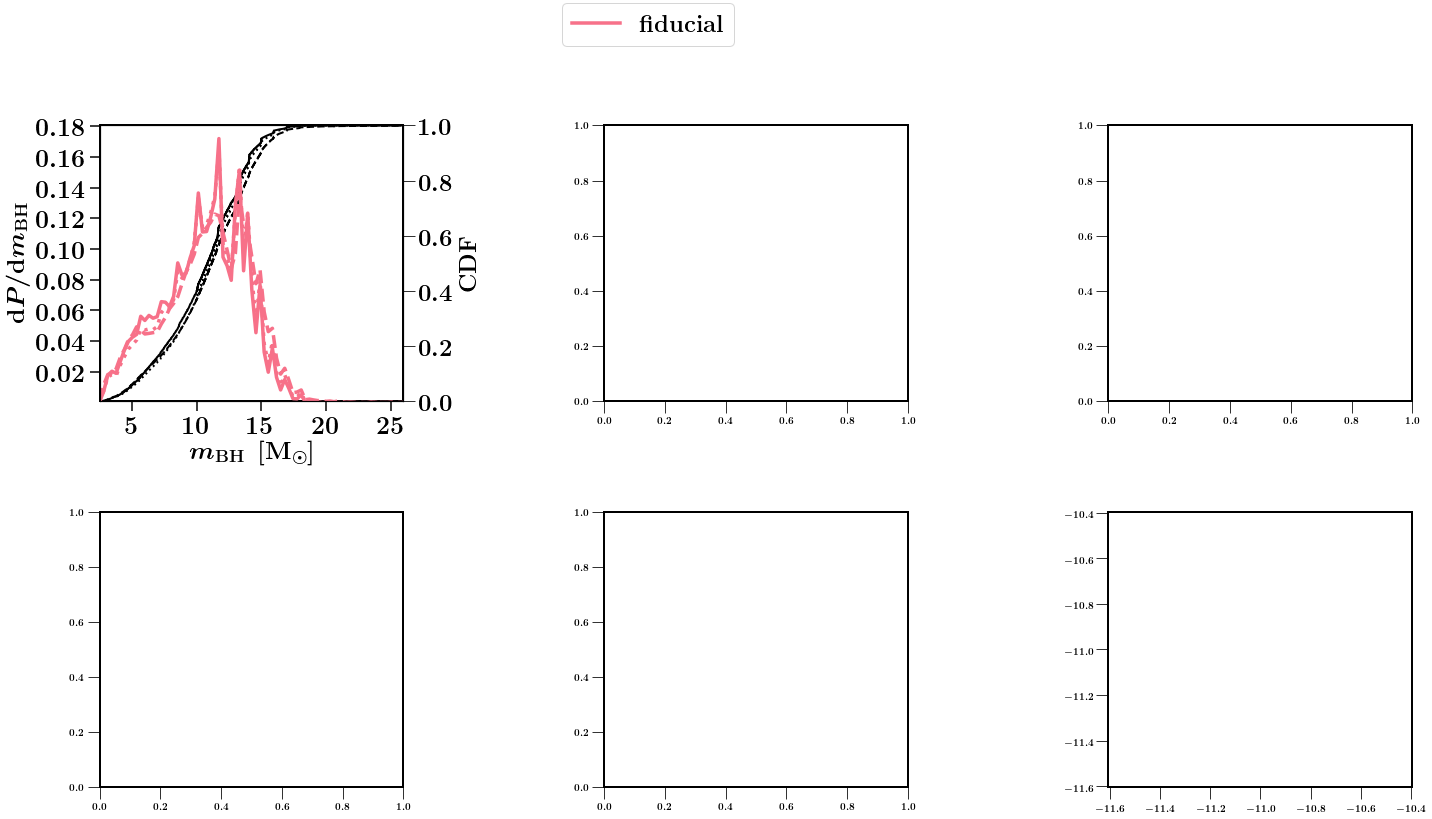
\includegraphics[width=1\textwidth]{../PlottingScripts/9_PredictedDistributions_BPS_and_MSSFR_variations/DistributionsModels_det_KDE.png} %
%
    \caption{Predicted distribution functions for the \Nmodels model variations for \bhnsSingle mergers. The distributions are weighted for the detection probability of a \ac{GW} detector network at design sensitivity. For each \bhnsSingle parameter we highlight the fiducial model (\mAzero) as well as model variations F and G. The distributions are plotted using a Gaussian kernel-density estimator with kernel bandwidths of as quoted in Table~\ref{tab:variations-BPS}. Only for the metallicities we use a different kernel density bandwidth of 0.1 for each model. }  
    \label{fig:Distributions_BHNS_kde}
\end{figure*}
%

\subsection{Predicted distribution functions}
%
%




\begin{figure*}
    \centering
%
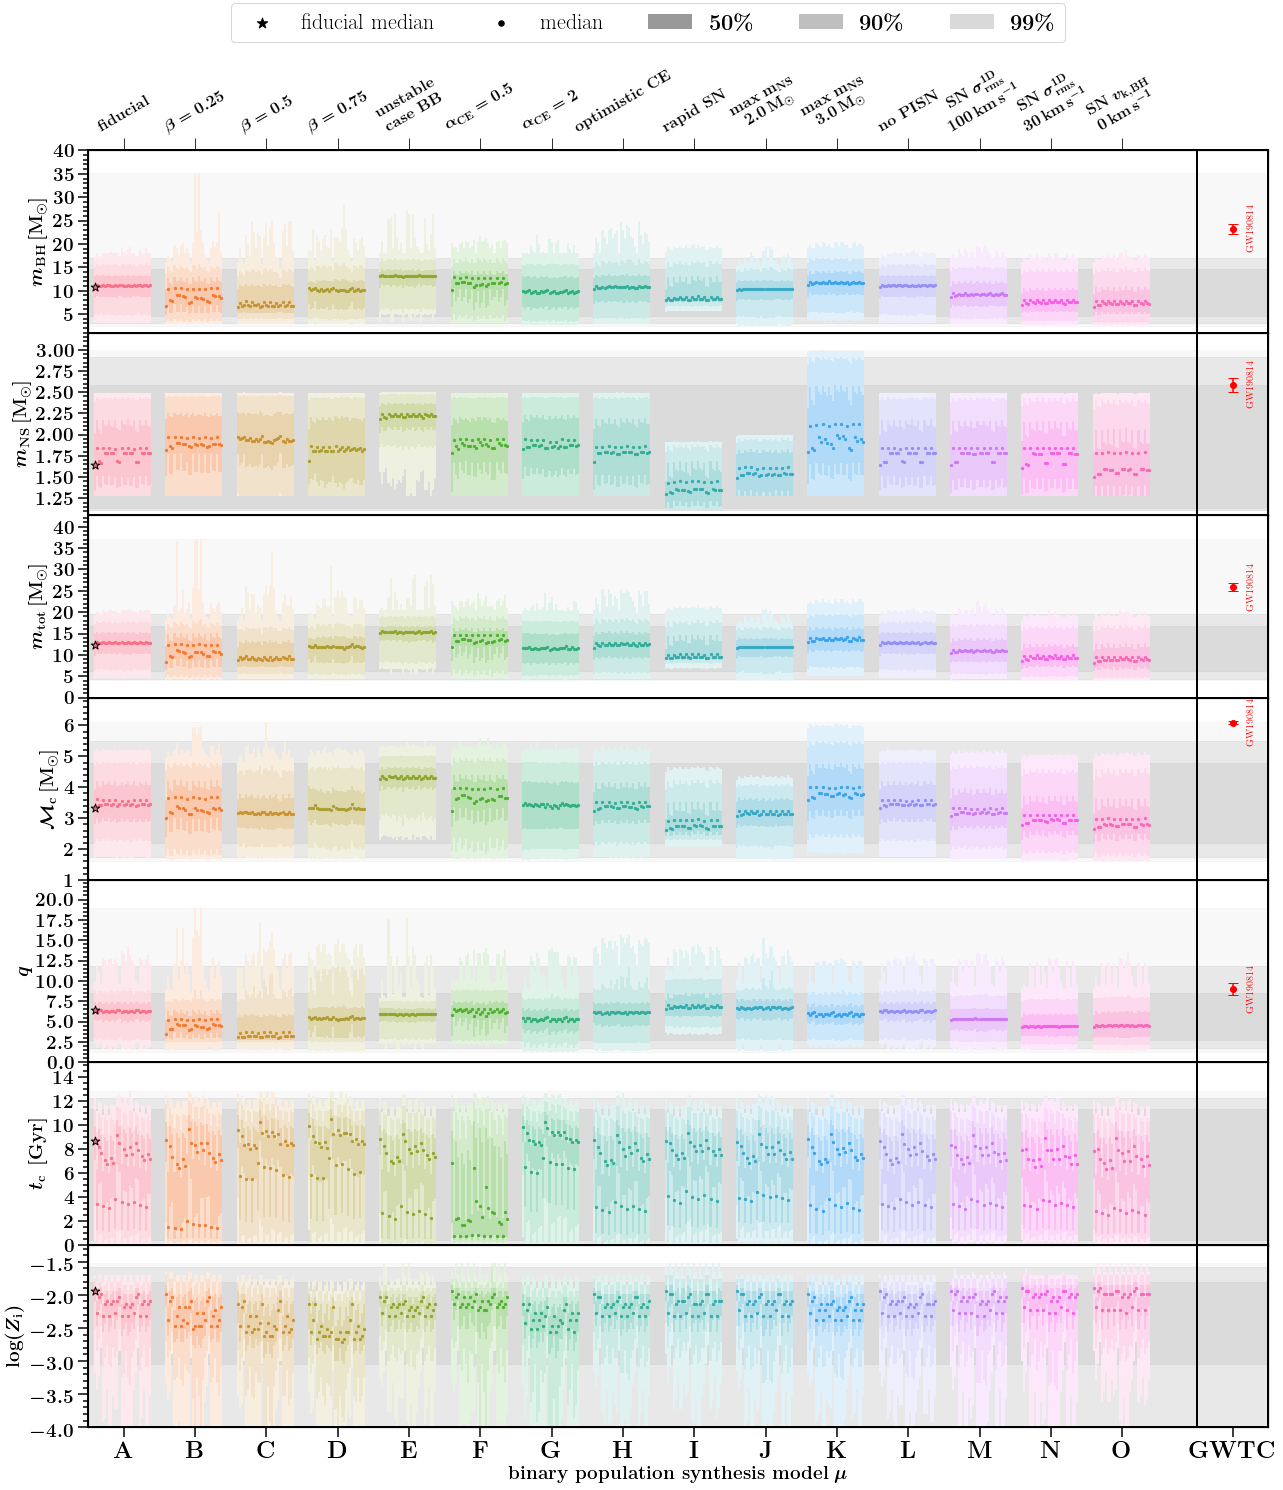
\includegraphics[width=1\textwidth]{../PlottingScripts/9_PredictedDistributions_BPS_and_MSSFR_variations/CDF_BPSandMSSFRvariations_Summary_BHNS_Z.pdf} %
%
    \caption{Confidence intervals for the predicted \bhnsSingle distributions for the variations of MSSFR and binary population synthesis models. 
    The distributions are weighted for the detection probability for a \ac{GW} network at design sensitivity. 
    For each binary population synthesis model we show for each \ac{MSSFR} variation the median (scatter points) and $90\%$ (dark colored bar) and $99\%$  (lighter colored bar) confidence intervals.  
    The gray areas show the range of the minimum and maximum 90$\%$ and 99$\%$ values over all model variations.
     The fiducial model (\mAzero) median values are shown with star symbols.   }
    %
    \label{fig:ConfidenceINtervals_BHNS}
\end{figure*}
%



\begin{figure*}
    \centering
%
\includegraphics[width=1\textwidth]{../PlottingScripts/9_PredictedDistributions_BPS_and_MSSFR_variations/PDF_BPSandMSSFRvariations_Summary_BHNS_Z.pdf} %
%
    \caption{Probability distribution functions for the predicted \bhnsSingle mergers  for the variations of MSSFR and binary population synthesis models studied in this paper. 
    The distributions are weighted for the detection probability for a \ac{GW} network at design sensitivity. 
    For each binary population synthesis model we show for each \ac{MSSFR} variation distribution function in a vertical bar. The color indicates the normalized probability of that bin.  }
    %
    \label{fig:PDF_BHNS}
\end{figure*}
%


In addition to the predicted rates, the shapes of the predicted \bhnsSingle distributions are sensitive to the binary population synthesis  and \ac{MSSFR} assumptions. To summarize and compare these effects, we discuss in this subsection the  shape of the \Nmodels distributions of the \bhnsSingle characteristics. We focus on showing the \bhnsSingle masses, mass ratio, total mass and chirp mass distributions as these are properties that will be measured by \ac{GW} observations. In addition, instead of the inspiral time we show the birth metallicity of the detected mergers.  The inspiral time and metallicity are highly correlated as mergers with longer inspiral times typically are formed with lower birth  metallicities. 


To summarize and compare the shape of the \Nmodels distributions we show three type of figures. First, Figure~\ref{fig:Distributions_BHNS_kde} shows all the predicted \bhnsSingle   distribution functions for our \Nmodels model variations on top of each other.   Second, Figure~\ref{fig:ConfidenceINtervals_BHNS} shows  the median and the $50\%$, $90\%$ and $99\%$ confidence intervals for  the predicted \bhnsSingle merger distributions. 
Finally,   Figure~\ref{fig:PDF_BHNS} shows the \Nmodels histograms for each of the   \bhnsSingle parameters in single bars next to each other.  The results for \ac{BHBH} and \ac{NSNS} mergers are discussed in Section~\ref{sec:comparing-with-BHBH-and-NSNS}.


% \ac{MSSFR}
% We also find that the median \ac{BH} mass could be used to rule out several binary population synthesis models (e.g. models such as A and F with median \ac{BH} mass around  versus models with a  low \ac{BH} mass.
%This is different compared to \ac{BHBH} mergers where typically have \acp{BH} masses well exceeding 20\Msun. 


\subsubsection{BH mass}
%
 Figure~\ref{fig:ConfidenceINtervals_BHNS} shows that in almost all of  our model variations  $90\%$ of the \bhnsSingle mergers have \ac{BH} masses  $\mbhf \sim [2.5, 17]\Msun$. We find that  most binary population models predict $<1\%$ of observed \bhnsSingle mergers will have \acp{BH} masses exceeding $\mbhf \gtrsim 20\Msun$. The exceptions are models B, I and J, where the $99\%$ confidence intervals reaches typically $25\Msun$ and model E where for one \ac{MSSFR} ($\rm{xyz}=231$) the $99\%$ confidence interval for $\mbhf$ reaches $30$\Msun. However, in those cases massive \acp{BH}   
 are still predicted to be rare among the  \bhnsSingle mergers. 
 Detecting more than 1$\%$ of   \bhnsSingle mergers with \ac{BH} masses exceeding $\approx 20$\Msun   would therefore support that a large fraction of the \bhnsSingle systems  formed from a different  formation channel such as in AGN disks or through dynamical formation, which predict a significant fraction of  \bhnsSingle mergers with  \acp{BH} exceeding 20\Msun \citep[][]{2020arXiv200302277R}.   Alternatively, it could constrain binary population synthesis and \ac{MSSFR} models as only a small fraction of our models is able to match such observations. 
 
Figure~\ref{fig:ConfidenceINtervals_BHNS} and Figure~\ref{fig:PDF_BHNS} also show that \bhnsSingle mergers with  $\mbhf \leq$5\Msun are  common  in most of the models. In all models, except models E (unstable case BB mass transfer) and F (rapid SN remnant mass model) the 90$\%$ confidence interval reaches below \mbhf $=5$\Msun. The sharp boundary in the minimum \ac{BH} mass for model F is caused by the rapid \ac{SN} remnant mass model, which assumes no \acp{BH} form with $\mbhf \leq 6\Msun$. Figure~\ref{fig:PDF_BHNS} shows that in models G, H, J and L detections of  \bhnsSingle mergers with $\mbhf \leq 6\Msun$   are most common.   


\subsubsection{NS mass}
The $90\%$ confidence intervals of the \bhnsSingle neutron star masses typically span a broad range  $\mnsf \sim [1.2, 2.3]$\Msun. Only  model  F (the rapid SN remnant mass model)  deviates drastically as the $90\%$ range shifts to $\mnsf \sim [1.1, 1.9]$\Msun and the most probable  \ac{NS} mass for \bhnsSingle mergers reaches below 1.2\Msun (see Figure~\ref{fig:PDF_BHNS}).
In most model variations we find  that the median \ac{NS} mass  is  $\gtrsim 1.8\Msun$ and that such massive \ac{NS} are thus common in \bhnsSingle mergers as can also be seen in the distribution functions. We show in Section~\ref{sec:comparing-with-BHBH-and-NSNS} that this is different to \acp{NS} in \ac{NSNS} mergers. 



\subsubsection{Total mass}
The \bhnsSingle total mass distributions follow the  \ac{BH} mass distributions as the \ac{BH} dominates the mass of the binary. Figure~\ref{fig:ConfidenceINtervals_BHNS}  shows that typically  $90\%$ of the predicted observed \bhnsSingle mergers will have $\mtotf  \sim [5, 18]\Msun$. 



\subsubsection{Chirp mass distribution}
Figure~\ref{fig:ConfidenceINtervals_BHNS} shows that  $90\%$ of the predicted observed \bhnsSingle mergers will have  $\mchirpf  \sim [1.7, 5]\Msun$.  The most probable chirp masses as shown in  Figures~\ref{fig:Distributions_BHNS_kde} and~\ref{fig:PDF_BHNS}, typically are in the range $\mchirpf \sim [2, 5]\Msun$. 

Figure~\ref{fig:PDF_BHNS} shows that both the total mass and chirp mass distributions are dissimilar between binary population synthesis models. The chirp mass and total mass  are one of the best constrained parameters from \ac{GW} observations.  This indicates that observations of \bhnsSingle mergers  are a good probe to distinguish between binary population synthesis models.  \floor{add how well chirp mass / total mass are measure, REFs??}


\subsubsection{Mass ratio distribution}
The $90\%$ confidence interval of the \bhnsSingle mass ratios $ (\qf \equiv \mbhf / \mnsf)$   is predicted in all models to  $\qf \sim [1, 12]$ (see  Figure~\ref{fig:ConfidenceINtervals_BHNS}). The median and most probable \bhnsSingle mass ratio for our fiducial model (A) is $\qf \approx 6$, but this moves as low as  $\qf \approx 2.5$ for models H, I and J   and as high as $\qf \approx 7$ for model F (see Fig.~\ref{fig:PDF_BHNS}).  Figure~\ref{fig:ConfidenceINtervals_BHNS} also shows  that in none of the models more than 1$\%$ of the \bhnsSingle mergers have mass ratios exceeding \qf $\geq 16$.  In addition, near equal mass ratios for \bhnsSingle mergers are rare.  We show in Section~\ref{sec:comparing-with-BHBH-and-NSNS} that  \ac{NSNS} and \ac{BHBH} mergers typically instead have $\qf \sim 1$. 


\subsubsection{Metallicities}
Figures~\ref{fig:ConfidenceINtervals_BHNS} and \ref{fig:PDF_BHNS} show that the range of the confidence intervals for the birth metallicities of the observed \bhnsSingle mergers strongly correlates with the \ac{MSSFR} prescription. This is mostly an effect from a combination of the \ac{MSSFR} prescriptions having different metallicity distributions in addition to the convolution with inspiral times from the \bhnsSingle mergers. Models with relatively higher metallicities origin from \ac{MSSFR} prescription that have the  \citet{2006ApJ...638L..63L} $+$ offset or \citet{2016MNRAS.456.2140M}  \ac{MZR} relation that for a given galaxy mass map to higher star formation metallicities.  
Figure~\ref{fig:PDF_BHNS} shows that typically the metallicities have values in the range $\log(\Zi/Z_{\odot}) \sim [-1, 0]$.
%(c.f.  \citealt[][]{2020arXiv200302277R}).  Progenitors for \bhnsSingle mergers with more massive \acp{BH}   typically lead to stellar mergers during the binary evolution.  
%This is different for  \ac{BHBH} mergers where the majority of predicted \acp{BH} exceed  $15$\Msun (see Appendix~\ref{sec:app-fiducial-GW-predictions-for-BBH-BNS}). 



\subsection{Effect from binary population synthesis and MSSFR variations on the shape of the distribution functions}
%

%\subsubsection{Effect from binary population synthesis variations}

We find that the variation in the predicted \bhnsSingle distribution functions is dominated by the binary population synthesis model. This can  be seen from the scatter in the median and  $50\%$ confidence intervals in Figure~\ref{fig:ConfidenceINtervals_BHNS} and especially by the variation in the probability distribution functions in Figure~\ref{fig:PDF_BHNS}, which are typically larger due to variations in binary population synthesis models compared to  \ac{MSSFR} variations. This is emphasized in Appendix~\ref{sec:app-Metallicity-density-function} where we  show in more detail that the normalized \bhnsSingle distributions are similar  under  \ac{MSSFR} variations. 
%with as example our Fiducial model. 

%Especially the total mass, chirp mass and \ac{BH} mass distributions of \bhnsSingle can be used to distinguish between models  
%
%The \ac{NS} mass distribution 


%
%From Figure~\ref{fig:ConfidenceINtervals_BHNS} and \ref{fig:PDF_BHNS} it is visible that especially the variation in binary population synthesis model dominates the   shape and typical values for the  predicted \bhnsSingle characteristics, whilst the change in \ac{MSSFR} relatively does not affect the distributions drastically.  
%





%%
%\begin{figure*}
%    \centering
%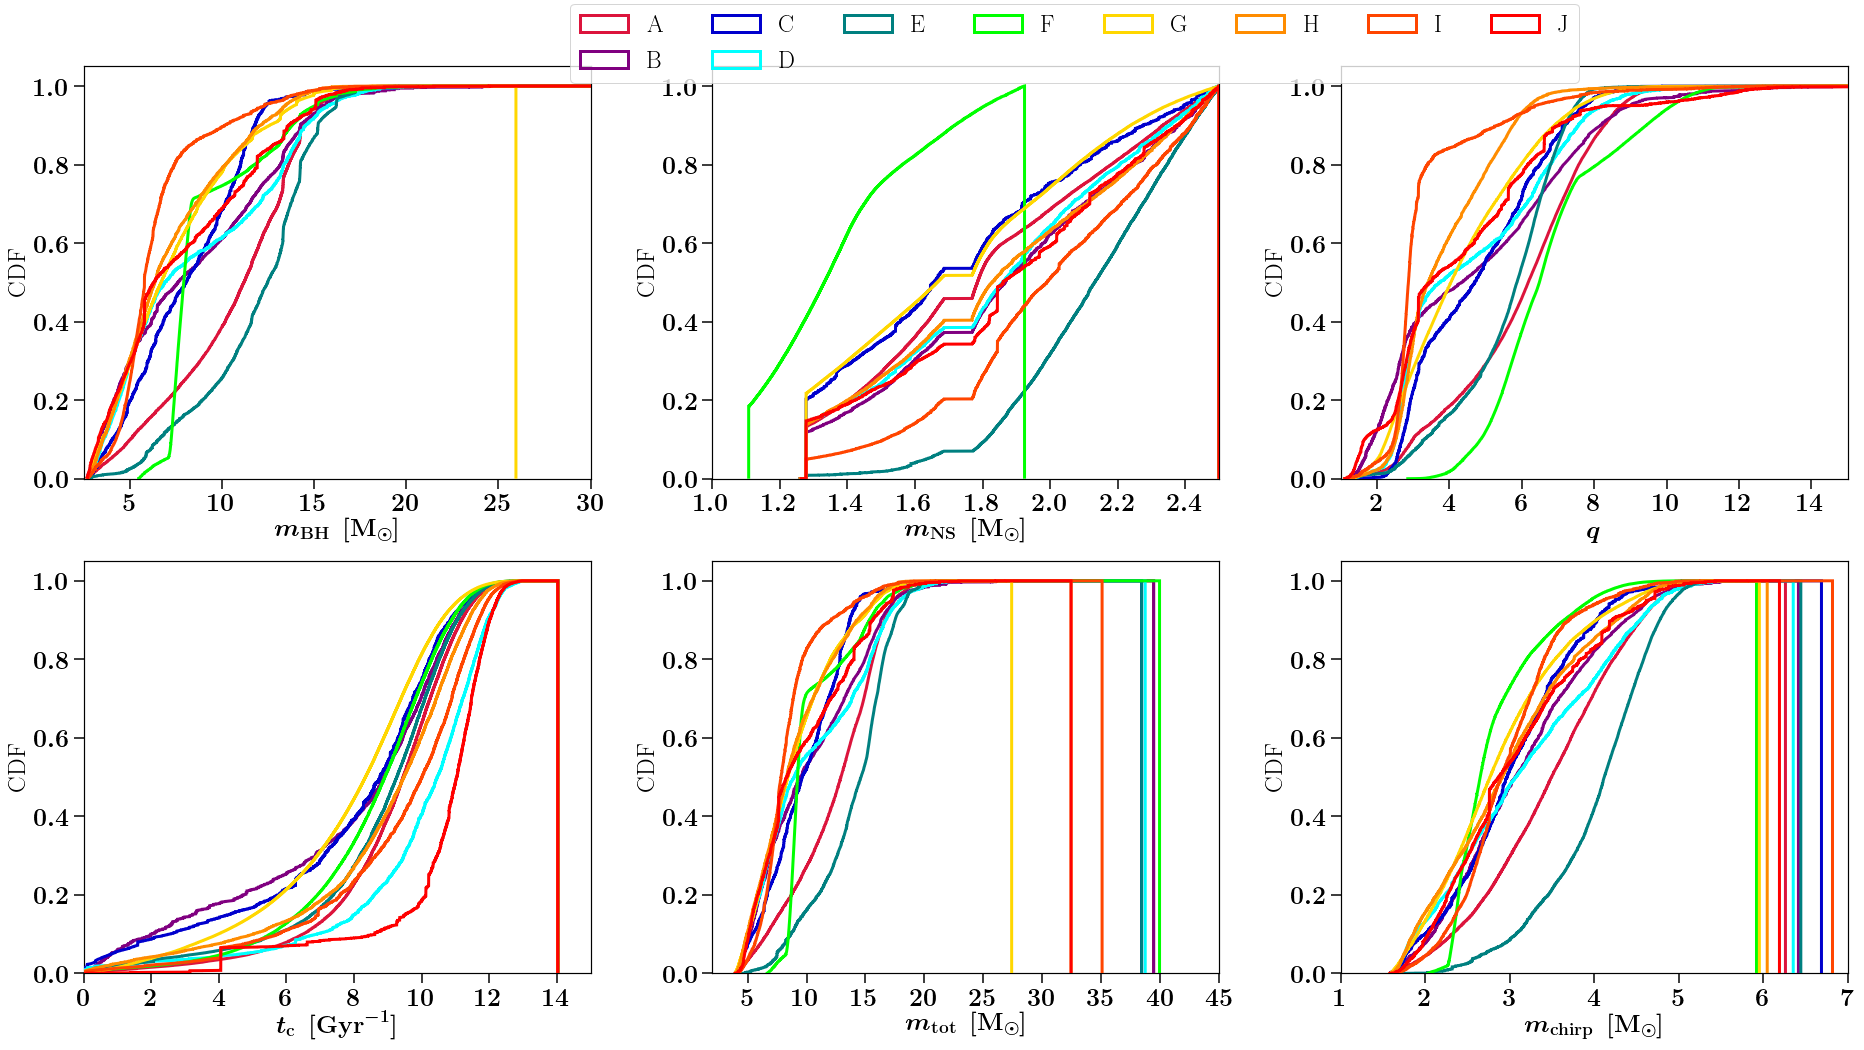
\includegraphics[width=1\textwidth]{../PlottingScripts/9_PredictedDistributions_BPS_and_MSSFR_variations/AllDistributions.png} %
%    \caption{}%
%    \label{fig:CDFs_BHNS_observed}
%\end{figure*}
%%
%
%




%%
%\begin{figure*}
%\label{fig:CDFs_BHNS_observed}
%    \centering
%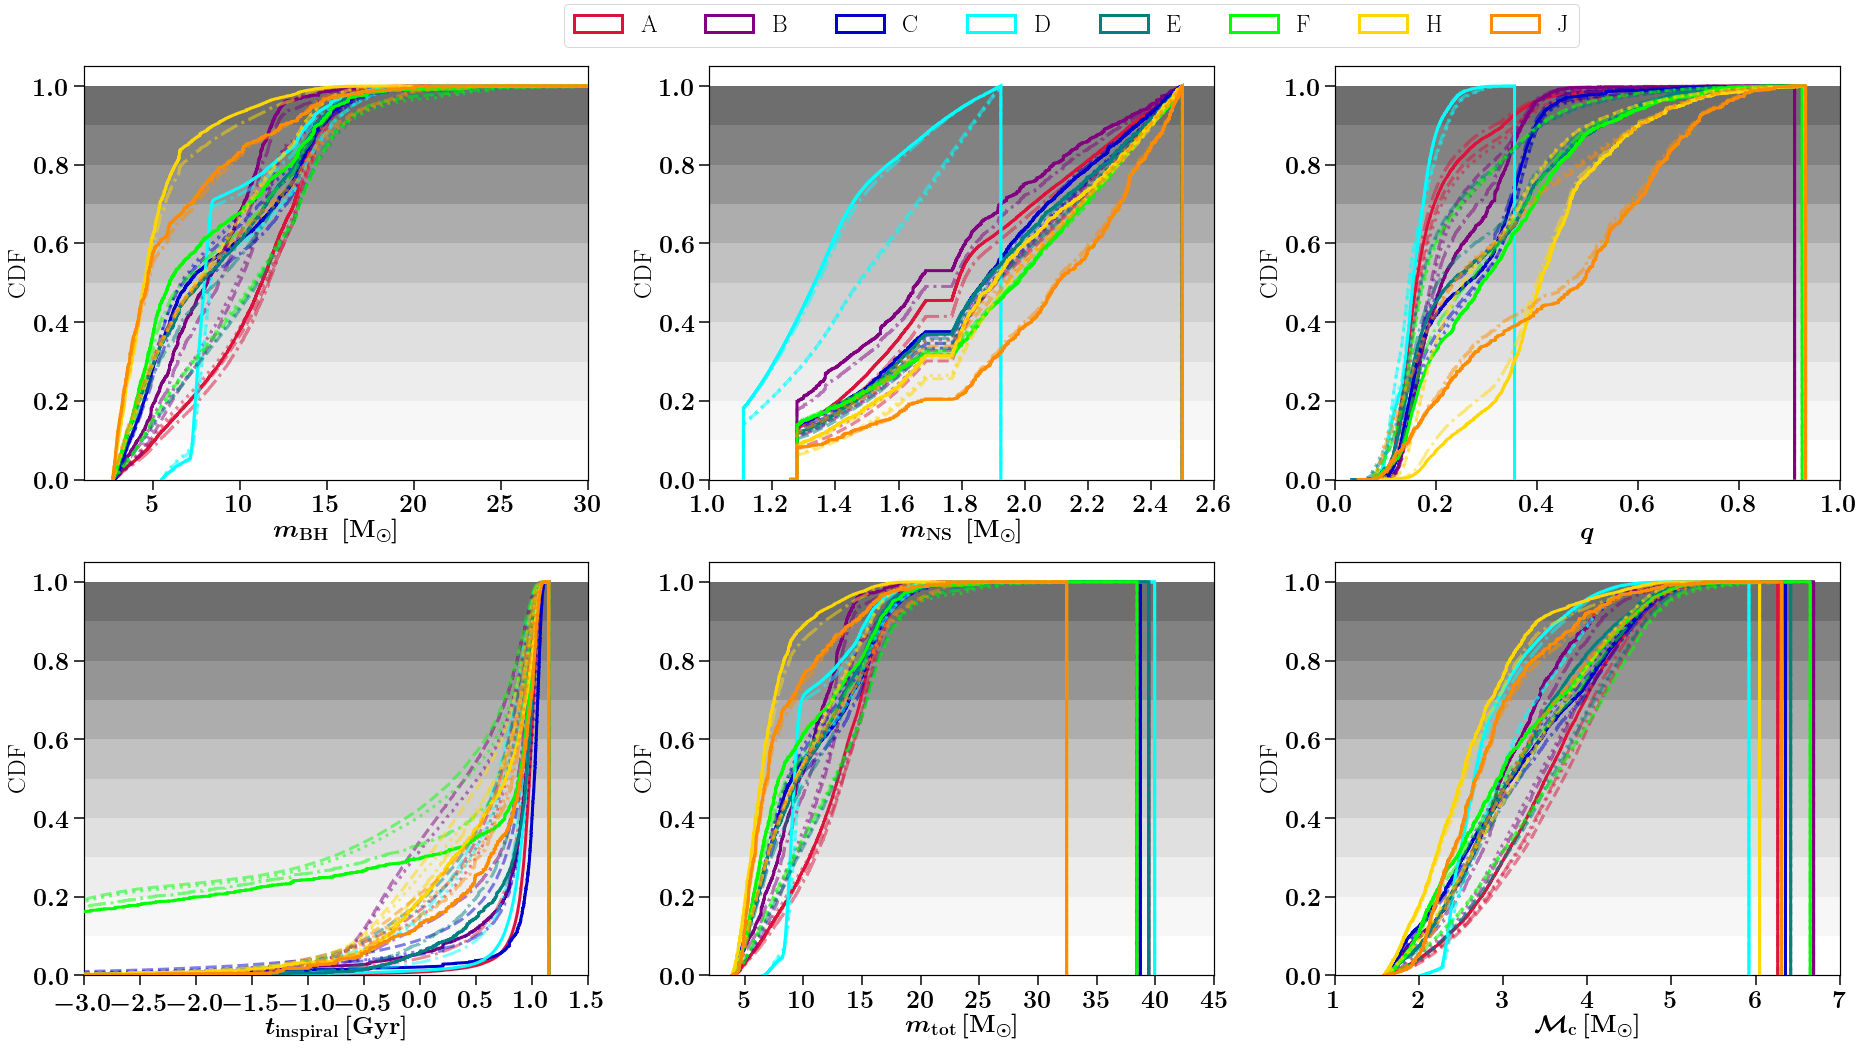
\includegraphics[width=1.0\textwidth]{../PlottingScripts/4_MSSFR_observed/DistributionsModels_observed_BHNS_CDF.pdf} %
%    \caption{}%
%\end{figure*}
%%







%%
%\begin{figure}
%    \centering
%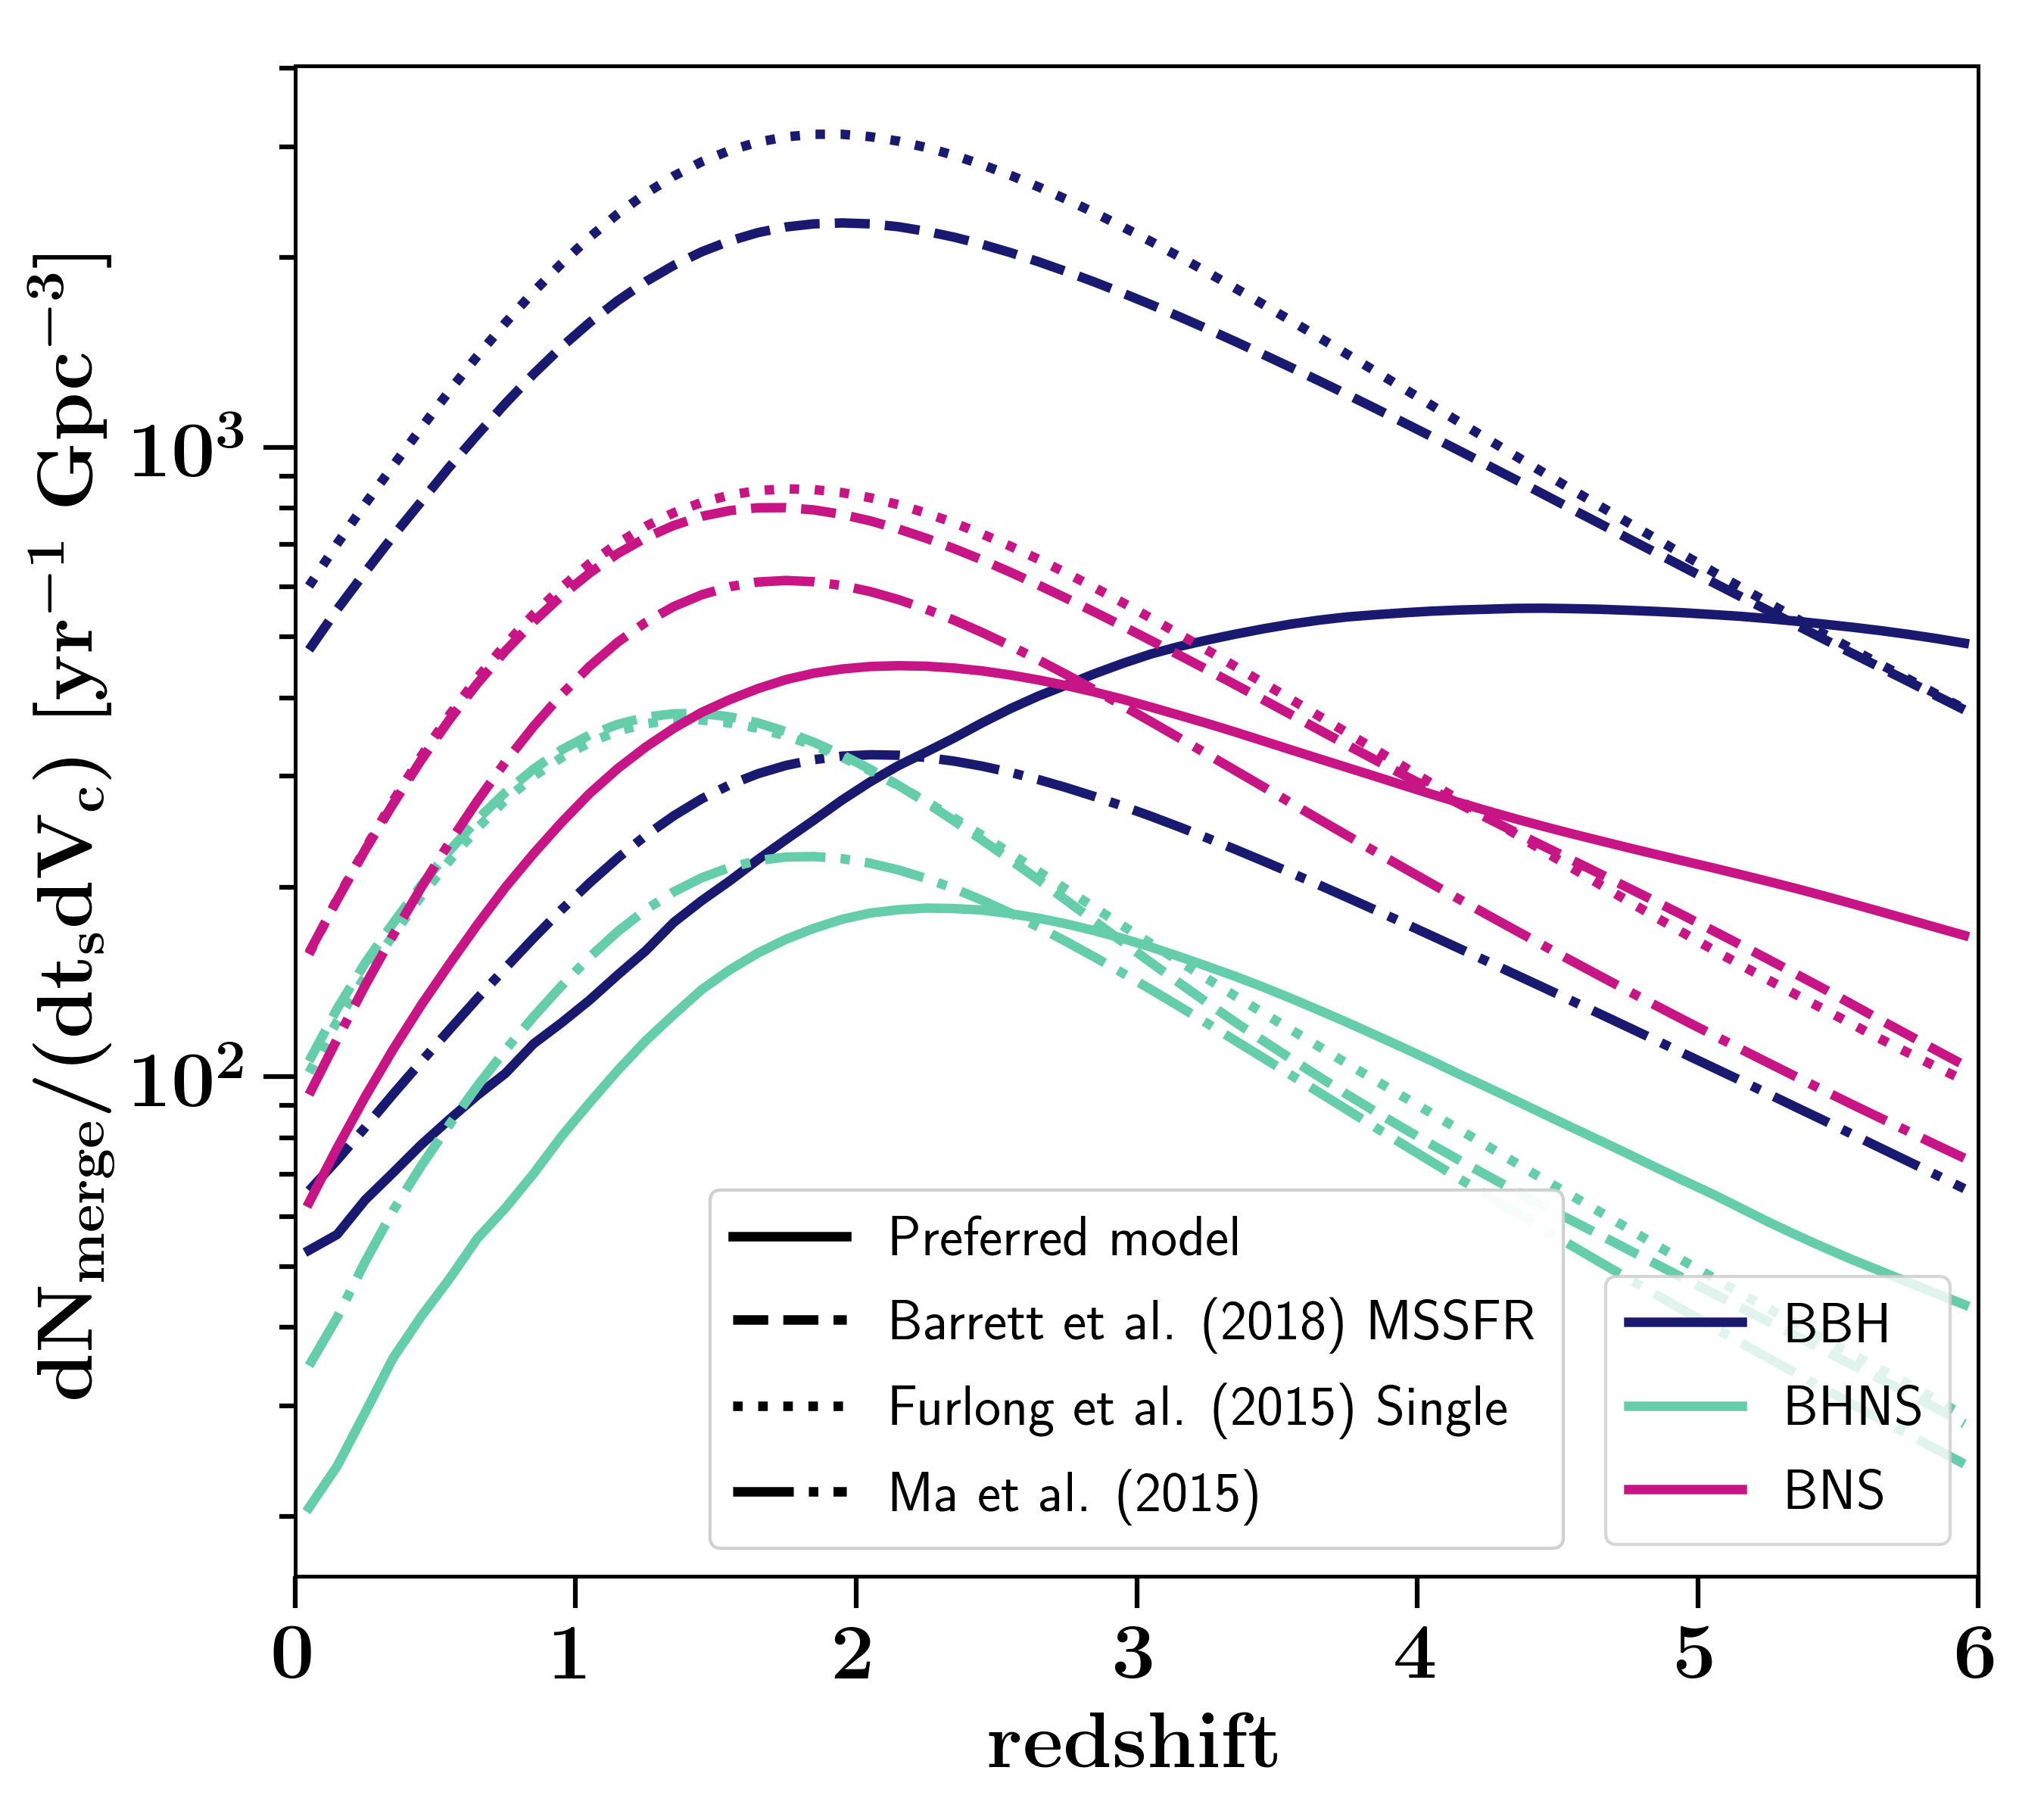
\includegraphics[width=1.0\columnwidth]{../PlottingScripts/5_DCOPerRedshift/TotalMergerRateRedshift.png} %
%
%\end{figure}
%%
%
%


%\begin{figure}
%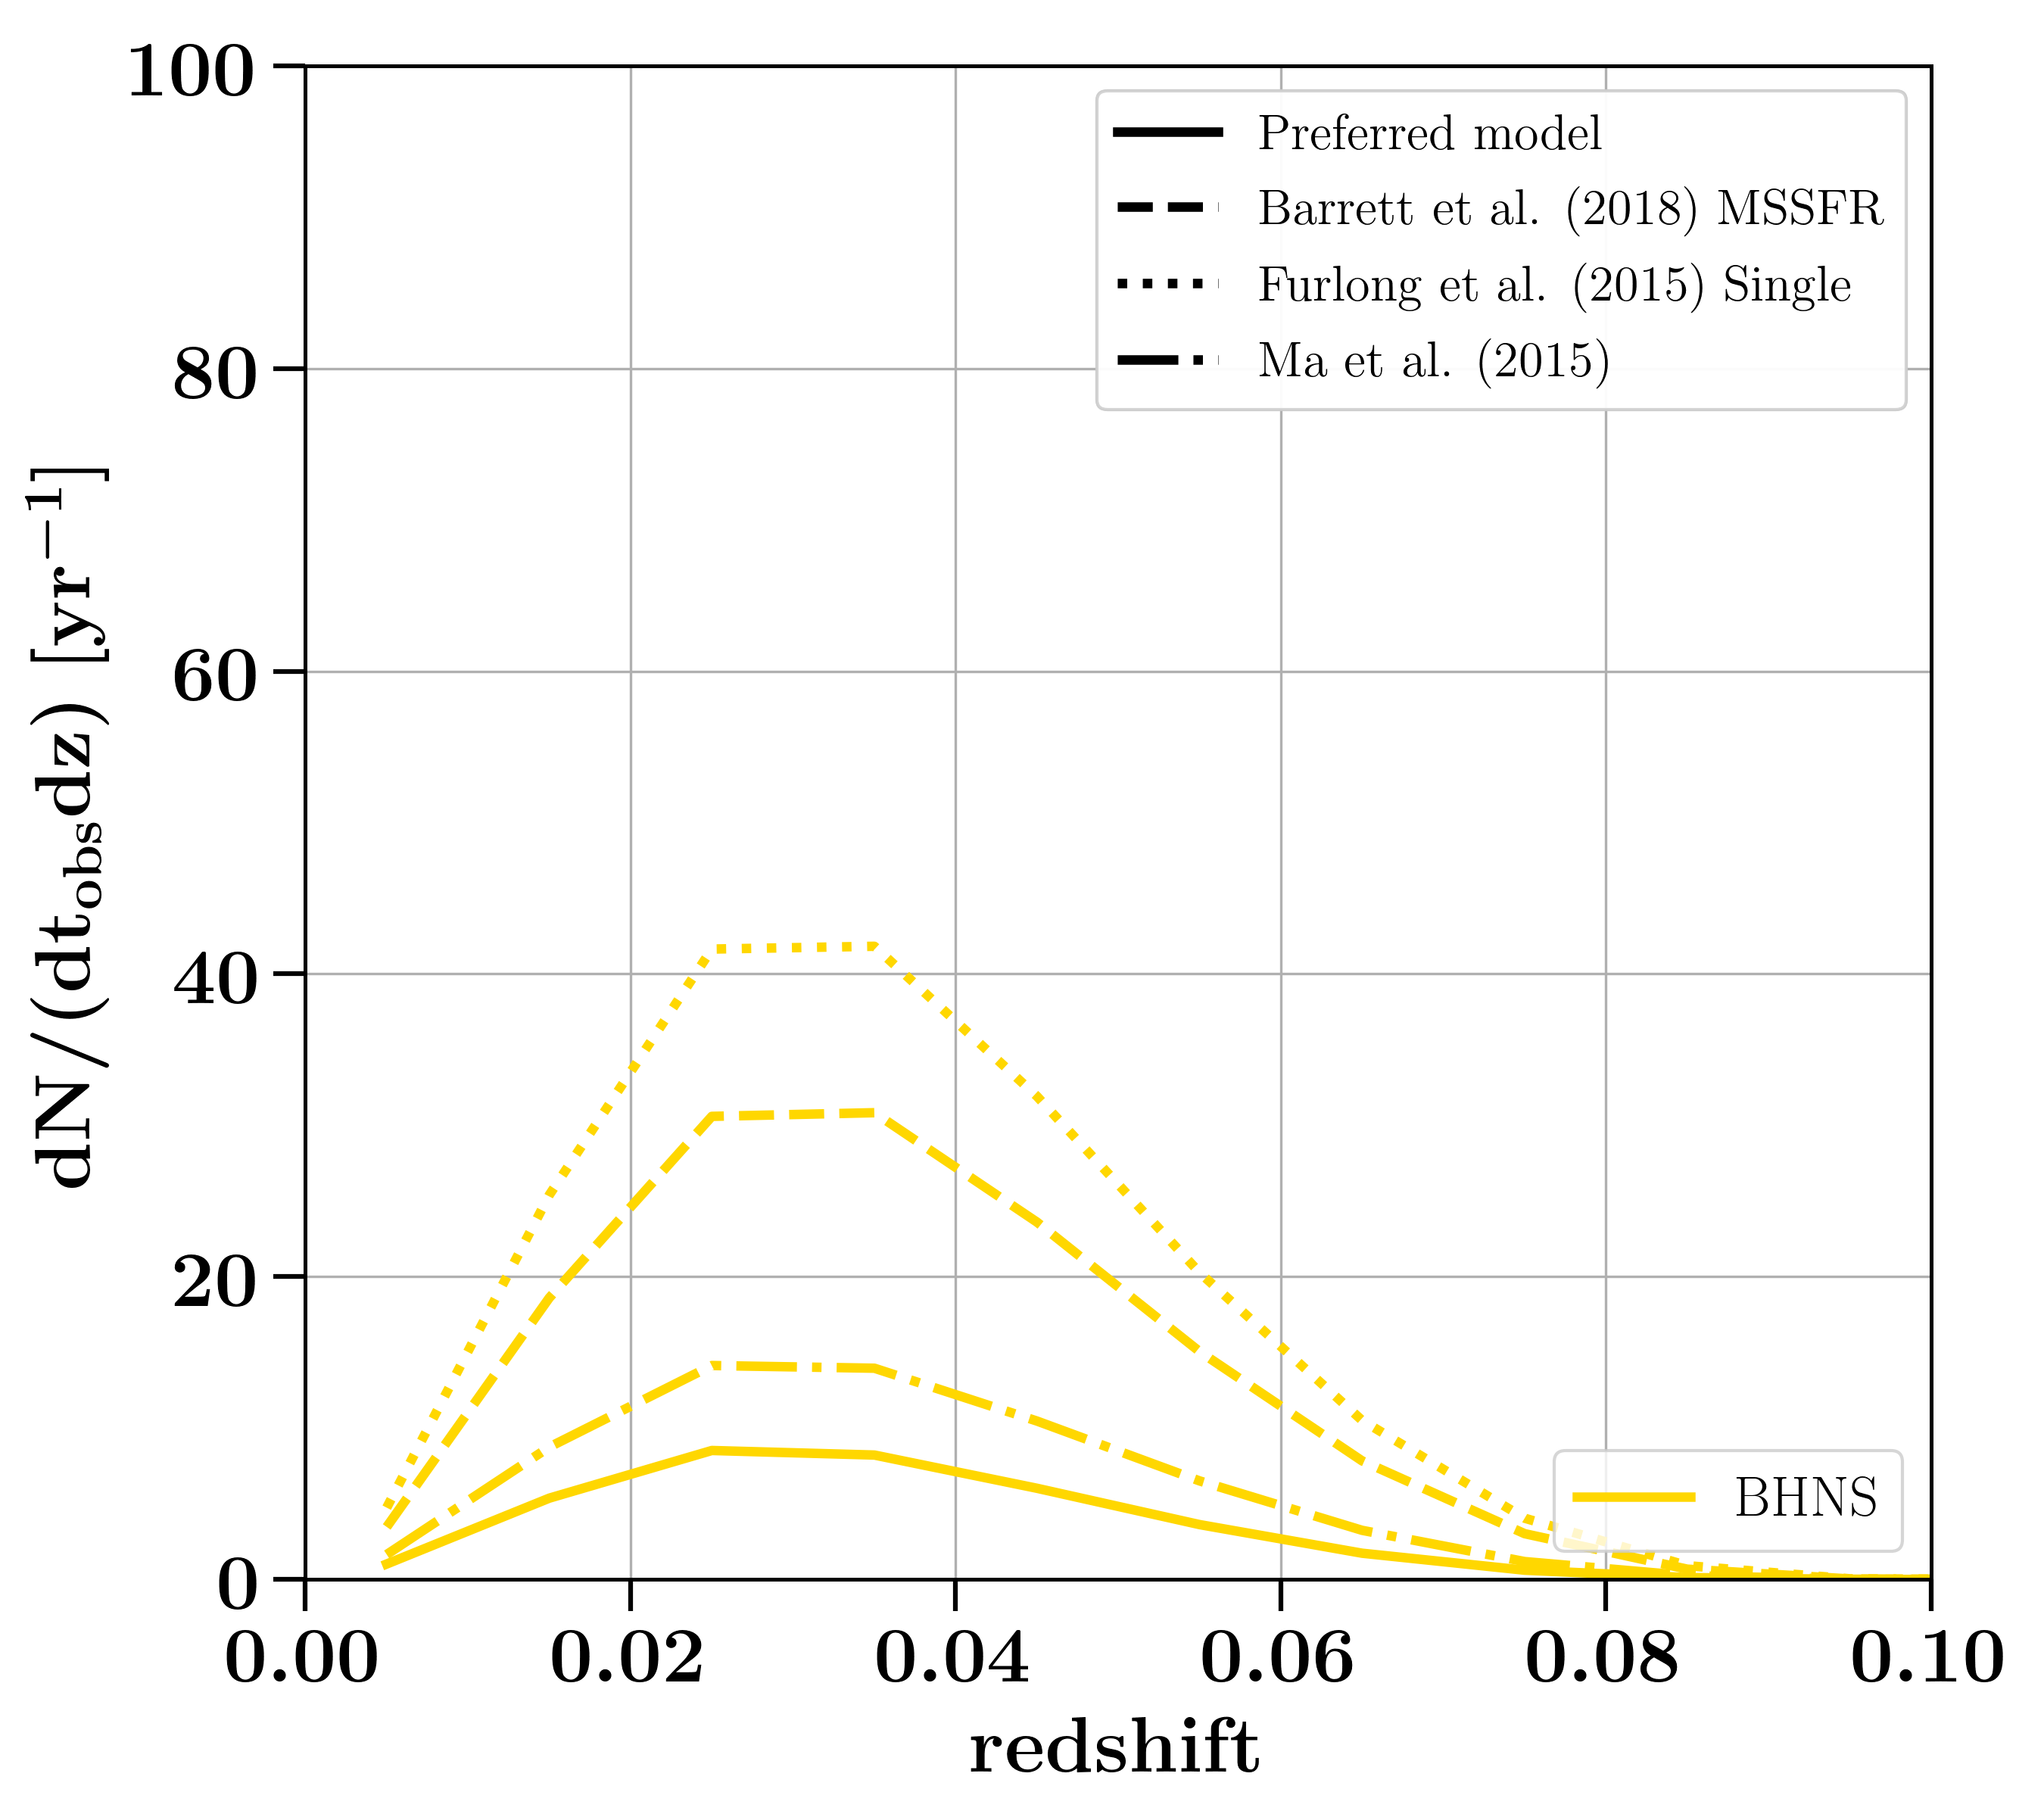
\includegraphics[width=1\columnwidth]{../PlottingScripts/4_MSSFR_observed/TotalMergerRateRedshiftObs-BHNS.png}
%   \caption{redshifts at which we will see \bhnsSingle mergers with LVK \ac{GW} network
%   }
%  \label{fig:BHNS_DCO_LVK-redshift}
%\end{figure}
%%

%\begin{figure}
%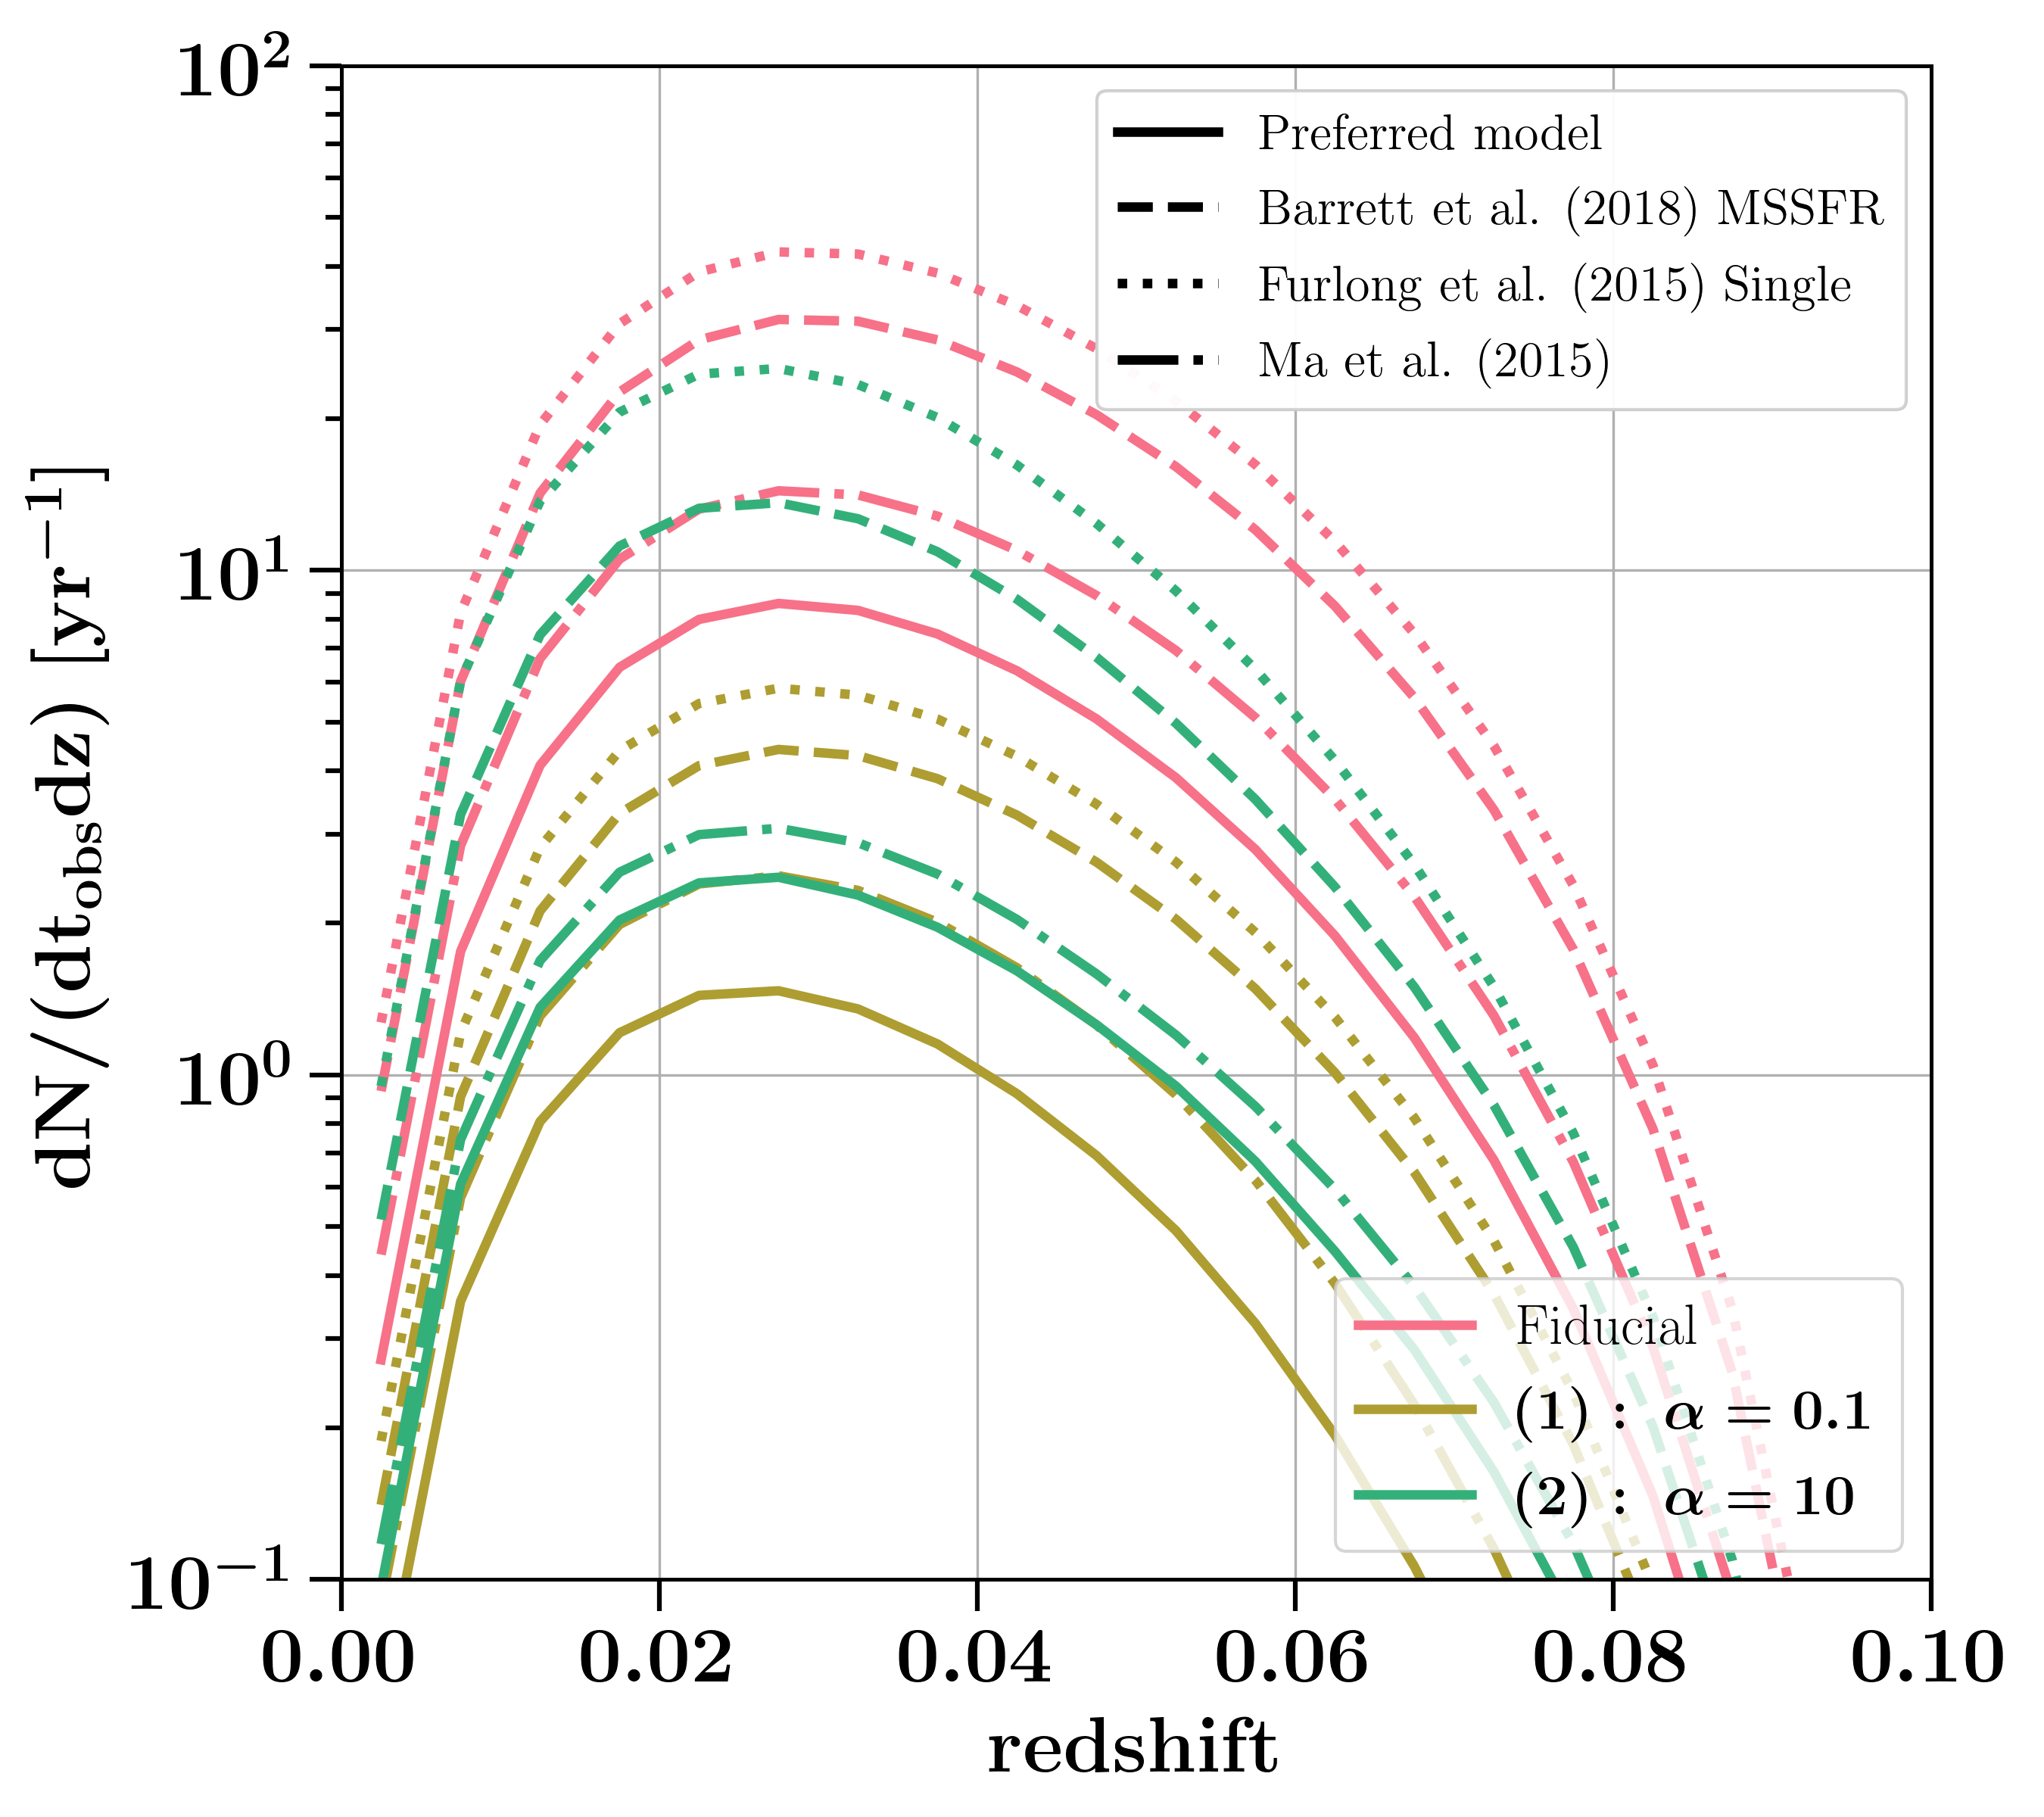
\includegraphics[width=1\columnwidth]{../PlottingScripts/4_MSSFR_observed/TotalMergerRateRedshiftObs-BHNS_models.png}
%   \caption{redshifts at which we will see \bhnsSingle mergers with LVK \ac{GW} network
%   }
%  \label{fig:BHNS_DCO_LVK-redshift}
%\end{figure}
%%


%\section{Other implications}
%
%
%\begin{itemize}
%	\item BH--Pulsar systems
%	\item LISA
%	\item UFD galaxies
%	\item 
%	\item Variations
%	\item 
%\end{itemize}

%%%%%% UFD: 

%% FROM MIKE ZEVIN

%ally (Qian &Woosley 1996; Thompson et al. 2001; Roberts et al. 2012; Martínez-Pinedo et al. 2012) and observation- ally (Wallner et al. 2015; Hotokezaka et al. 2015) as a pro- duction site for heavy r-process elements. The neutron-rich ejecta from neutron-star mergers (NSMs) is theorized to fill these open gaps in the periodic table, polluting the Uni- verse with the heaviest naturally-occurring elements (Lat- timer & Schramm 1974, 1976; Eichler et al. 1989; Meyer 1989; Davies et al. 1994; Ruffert et al. 1997; Rosswog & Liebend 1999; Freiburghaus et al. 1999). Over

%A number of observational campaigns have investigated
%the ubiquity of r-process enhancement in GCs. From a sam- ple of 11 low-metallicity GCs, Roederer (2011) found that 4 GCs showed clear signs of large r-process dispersion, 5 GCs showed no dispersion, and 2 GCs were more ambigu- ous with smaller levels of dispersion. Out of the 5 GCs that had no clear r-process dispersion, 2 show bimodal chemi- cal abundance ratios, possibly suggesting formation through the merger of 2 separate GCs that may have washed out ini- tial star-to-star dispersion (Yong & Grundahl 2008; Marino et al. 2009; Carretta et al. 2010).



\section{Comparison with \ac{BHBH} and \ac{NSNS} mergers}
\label{sec:comparing-with-BHBH-and-NSNS}
%
Ground-based \ac{GW} detectors observe all three flavors of \ac{DCO} mergers. In this section we discuss the  predictions for the rate and characteristics of \ac{NSNS} and \ac{BHBH} mergers for our set of \Nmodels models (see Table~\ref{tab:variations-BPS-BHBH-NSNS}). We  compare our predictions for \ac{BHBH} and \ac{NSNS}  mergers with the results we obtained for \bhnsSingle mergers in the previous section and in particular focus on what we can learn about  the binary population synthesis  and \ac{MSSFR} uncertainties from each population. 




\subsection{Intrinsic merger rates}
\label{subsec:comparing-BBH-BNS-intrinsic-rates}
%
Figure~\ref{fig:IntrinsicRatesBBHBNSBHNS} shows the predicted intrinsic merger rates for BHBH, \ac{NSNS} and \bhnsSingle mergers. 
We find $\rate_{\rm{m}}^{0,\rm{BHBH}} \sim [ \RateIntrinsicAzeroBHBHmin,  \RateIntrinsicAzeroBHBHmax]$\GpcminThree \yearmin and   $\rate_{\rm{m}}^{0,\rm{NSNS}} \sim [ \RateIntrinsicAzeroNSNSmin,  \RateIntrinsicAzeroNSNSmax]$\GpcminThree \yearmin. Our fiducial model predicts merger rates of  $\rate_{\rm{m}}^{0,\rm{BHBH}} \approx  \RateIntrinsicAzeroBHBH$\GpcminThree \yearmin and  $\rate_{\rm{m}}^{0,\rm{NSNS}} \approx  \RateIntrinsicAzeroNSNS$\GpcminThree \yearmin for \ac{BHBH} and \ac{NSNS} mergers respectively. 


Many of the  predicted rates in Figure~\ref{fig:IntrinsicRatesBBHBNSBHNS} are inconsistent with the observed $90\%$ confidence intervals from \ac{GW} observations from \citep{2019PhRvX...9c1040A,2020arXiv200101761T}. 
First, a large subset of the \ac{MSSFR} variations overpredicts the  \ac{BHBH} merger rate for all binary population synthesis model variations. An example is \ac{MSSFR} model $\rm{xyz} =231$, which is highlighted. These are the \ac{MSSFR} models that have the  \citet{2006ApJ...638L..63L}   MZR, which corresponds to star formation with relatively low metallicities  compared to the other MZRs, which increases the formation of \ac{BHBH} mergers (see also Section~\ref{subsec:effect-from-MSSFR-variations}).
Secondly,   almost all  predicted \ac{NSNS} merger rates  are below the observed 90$\%$ confidence interval.  
 This finding is similar to other work on the isolated binary evolution channel  \citep[e.g.,][]{2018MNRAS.474.2937C}. This could indicate  that the observed rate estimate from \ac{GW} observations might be an over-prediction caused by the small number of detections. This is especially likely since the current \ac{NSNS} constrained rate from \ac{GW}  observations is also higher compared to estimates from short gamma-ray bursts and the galactic \ac{NSNS} population. For example the lower limits from short gamma-ray burst, pulsar and kilonovae constraints range in $\rate_{\rm{m, min}}^{0,\rm{NSNS}} [50, 90]\GpcminThree \yearmin$ \citep{2012MNRAS.425.2668C, 2013ApJ...767..140P,2015ApJ...815..102F,2016NatCo...712898J} which is significantly lower compared to the lower limit of $\approx 200\GpcminThree \yearmin$ from \ac{GW} observations and would make most of our model predictions, except those from model E,  consistent with the constrains from observations.  
  Alternatively,   our binary population synthesis models might underestimate the efficiency of \ac{NSNS} merger formation. Examples could be that  binary population synthesis underestimates the expansion of low mass stars that lead to NSs \citep{2020arXiv200301120L}, that our binary population synthesis do not treat the stellar winds or mass transfer stability correctly,  or that our remnant mass prescription underestimates the fraction of \ac{NS} formation. Future studies should explore the impact of such uncertainties on the rates for all three types of \ac{DCO} mergers and whether future  constrains from observation are still in contradiction with the rate predictions. 
  See \citet{2018MNRAS.474.2937C} for a further discussion on this challenge. 
% \floor{add sGRB lines?}
%  Or because \ac{CE} is more efficient .  \floor{add sGRB lines}. We note that the \ac{GW} observed rates for  \ac{NSNS} mergers are larger compared to estimates from pulsars, 
 
 
% \floor{discuss sGRBs etc}
 

%
\begin{table}
\caption{List of the \NmodelsBPS binary population synthesis models simulated in this study. \\
 $^{*}$total number of data points in the combined simulation over 50 metallicity bins that consist of a \bhnsSingle  system that mergers in a Hubble time.}
\label{tab:variations-BPS-BHBH-NSNS}
\resizebox{\columnwidth}{!}{%
\centering
\begin{tabular}{lllrr}
\hline
$m$ 	& Physics that is changed & Variation  			& $\#$BHBH$^{*}$    & $\#$NSNS$^{*}$ 	\\ \hline
%
A      		& fiducial model        		& -     					& $ 7\,373\,980 $   & $588\,645$ 	\\
%
B      		&  \ac{CE}       		& optimistic     					& $7\,779\,848  $ & $633\,264$  	\\
%
C       		& \ac{CE}                    				& $\alpha = 0.5$ 	& $6\,962\,153 $ 	& $346\,757$ 	\\
%
D       		& \ac{CE}                    				& $\alpha = 2$  	& 	$  5\,567\,997$ & $1\,227\,670$	\\
%
E       		& case BB mass transfer 	& Unstable 			&   $8\,962\,233  $&  $1\,207$  \\
%
F       		& SNe                   				& Fryer rapid   		&  $ 6\,924\,908$ & $382\,295$  \\
%
G       		& SNe                   				& no \ac{BH} kick   		& $7\,608\,256$  & $1\,974\,997$  \\
%
H       		& mass transfer                  				& $\beta=0.25$  		& $7\,834\,458$ & $93\,469$ \\ 
%
I       		& mass transfer                  				& $\beta=0.5$  		&  $5\,840\,645$ &  $210\,071$ \\ 
%
J       		& mass transfer                  				& $\beta=0.75$  		& $4\,687\,882$ &  $883\,659$ \\ 
%
K      		& SN                 				& $\sigma=100$\kms  		& $6\,602\,452 $ & $1\,085\,652$ \\  
%
L       		& SN                  				& $\sigma=30$\kms  		& $ 6\,388\,040 $  & $1\,862\,721$  \\ 
\hline
\end{tabular}%
}
\end{table}


 

%%
\begin{figure*}
    \centering
%\includegraphics[width=1.0\textwidth]{../PlottingScripts/8_PredictedRates_BPS_and_MSSFR_variations/Rates_intrinsic_analysisFiducialMSSFR_linestyleColouring.png}
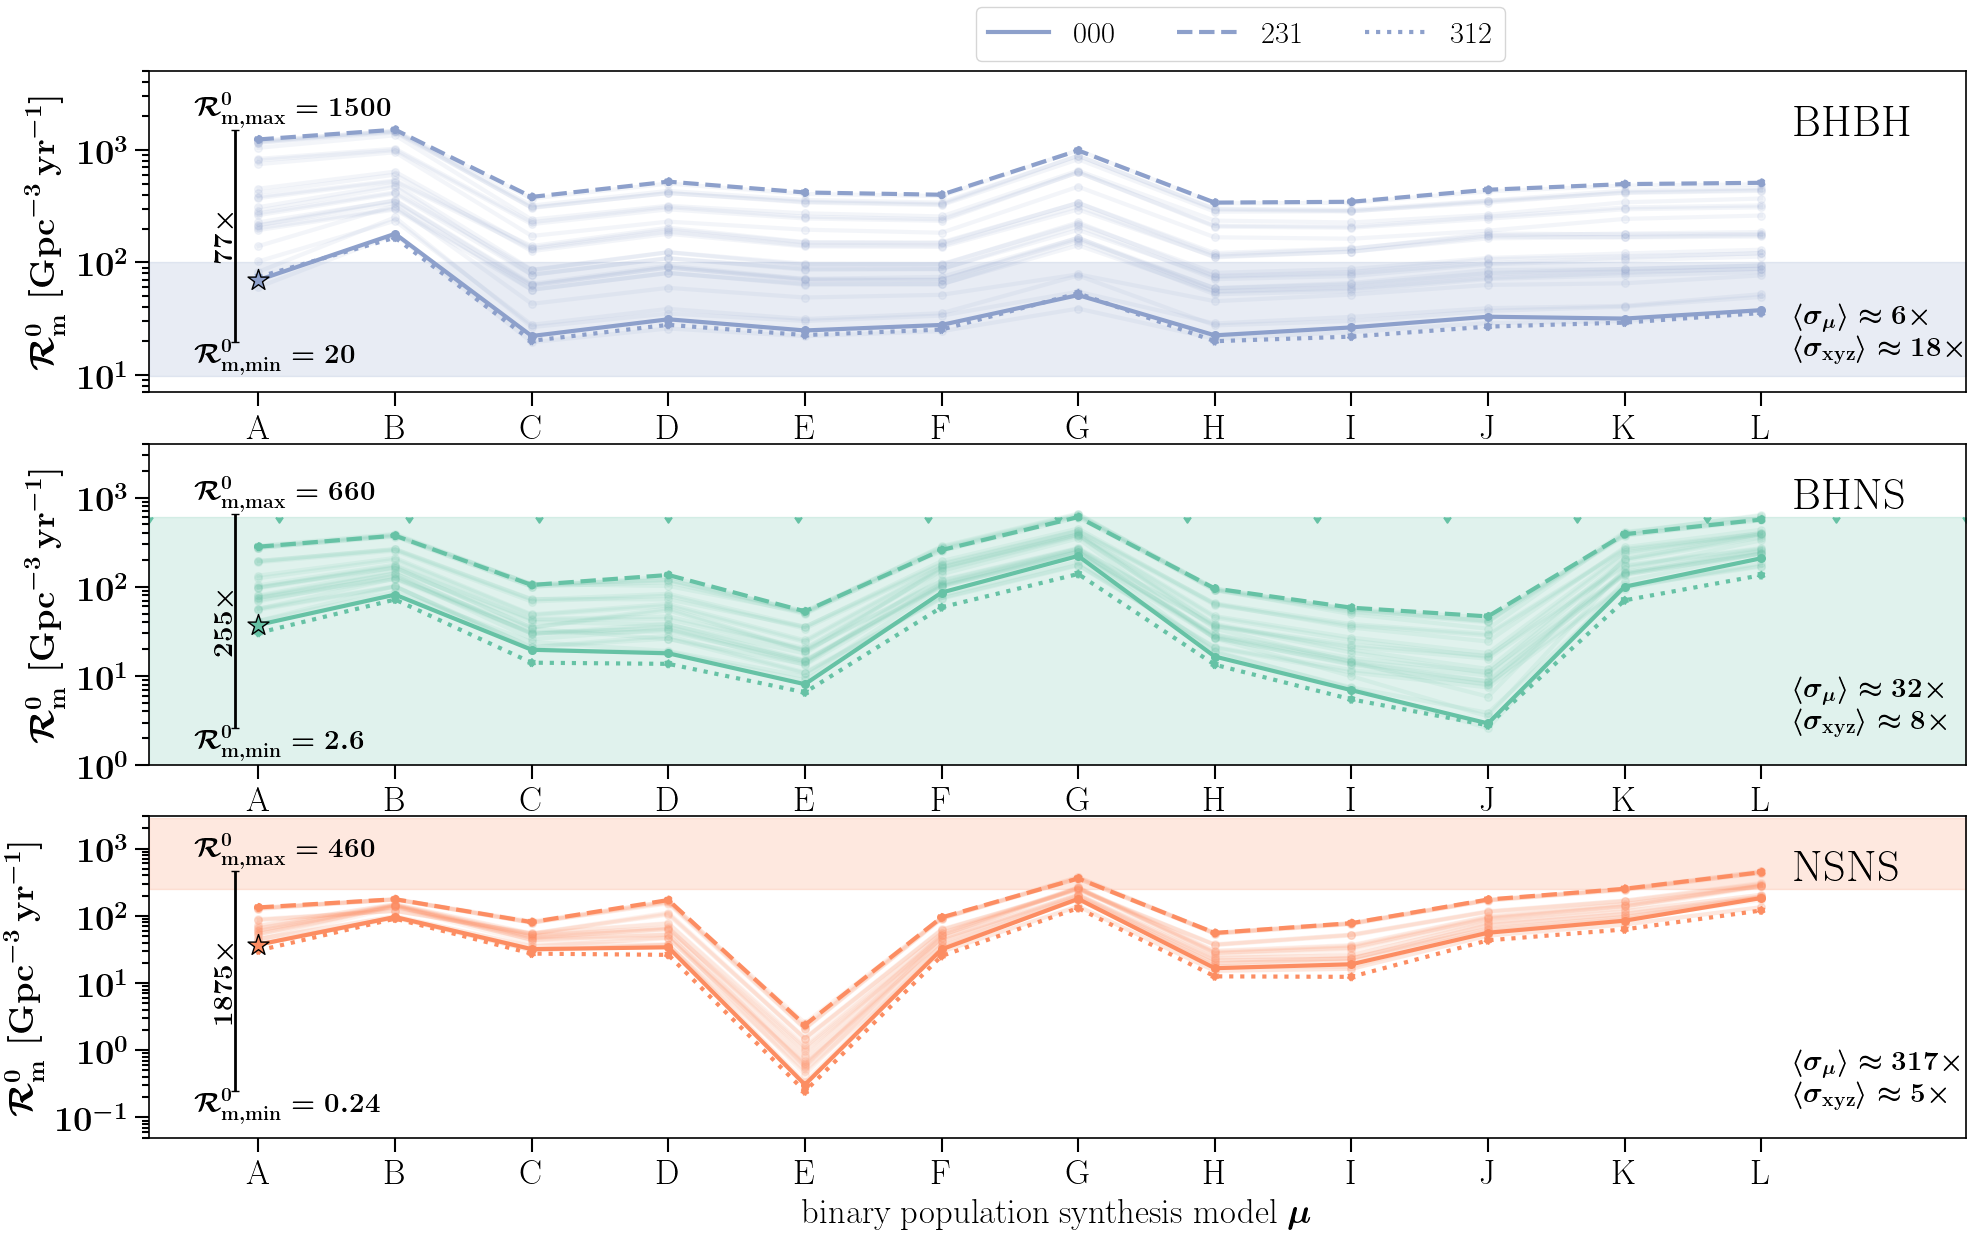
\includegraphics[width=1.0\textwidth]{../PlottingScripts/8_PredictedRates_BPS_and_MSSFR_variations/Rates_intrinsic_AllDCO.png}
\caption{Same as Figure~\ref{fig:IntrinsicRates} but for \ac{BHBH} (top panel), \bhnsSingle (middle panel) and \ac{NSNS} mergers (bottom panel). \question{the middle panel is the same as Fig.~\ref{fig:IntrinsicRates} should I keep the BHNS also here? If not, should I keep Fig.~\ref{fig:IntrinsicRates} the way it is or instead replace with this middle panel (green color)?} } 
 %
%    \caption{Predicted intrinsic rates of BHBH,  BHNS and \ac{NSNS} mergers for different population synthesis and MSSFR models (summarized in Table~\ref{tab:variations-BPS}, \ref{tab-MSSFR-variations-labels}).  
%    The rates are for mergers at redshift $z=0$ without applying \ac{GW} selection effects. 
%    For each binary population synthesis model the figure shows rates for the 28 variations in \ac{MSSFR} (Table~\ref{tab-MSSFR-variations-labels}). Four \ac{MSSFR} variations are highlighted.  In the background of each panel the  $90\%$ confidence interval for the observed rate by \citep{2019PhRvX...9c1040A,2020arXiv200101761T} are shown, where the \bhnsSingle is an upper limit. Our fiducial model  (\mAzero) estimates are shown with star symbols. On the right of each panel  $\langle \sigma_{\mu}\rangle$ and $\langle \sigma_{\rm{.x.y.z}}\rangle$ represent the mean scatter  in  rates caused over binary population synthesis and \ac{MSSFR} variations respectively. The minimum and maximum rates as well as the ratio between those are quoted for each merger type. We use the short-hand notation $\rate_{\rm{m}}^0 \equiv (\diff \Ndet^2 / \diff \ts \diff \Vc)(\tmerger(z=0))$. }%
\label{fig:IntrinsicRatesBBHBNSBHNS}
\end{figure*}
%

\subsection{Observed merger rates}

%
\begin{figure*}
    \centering
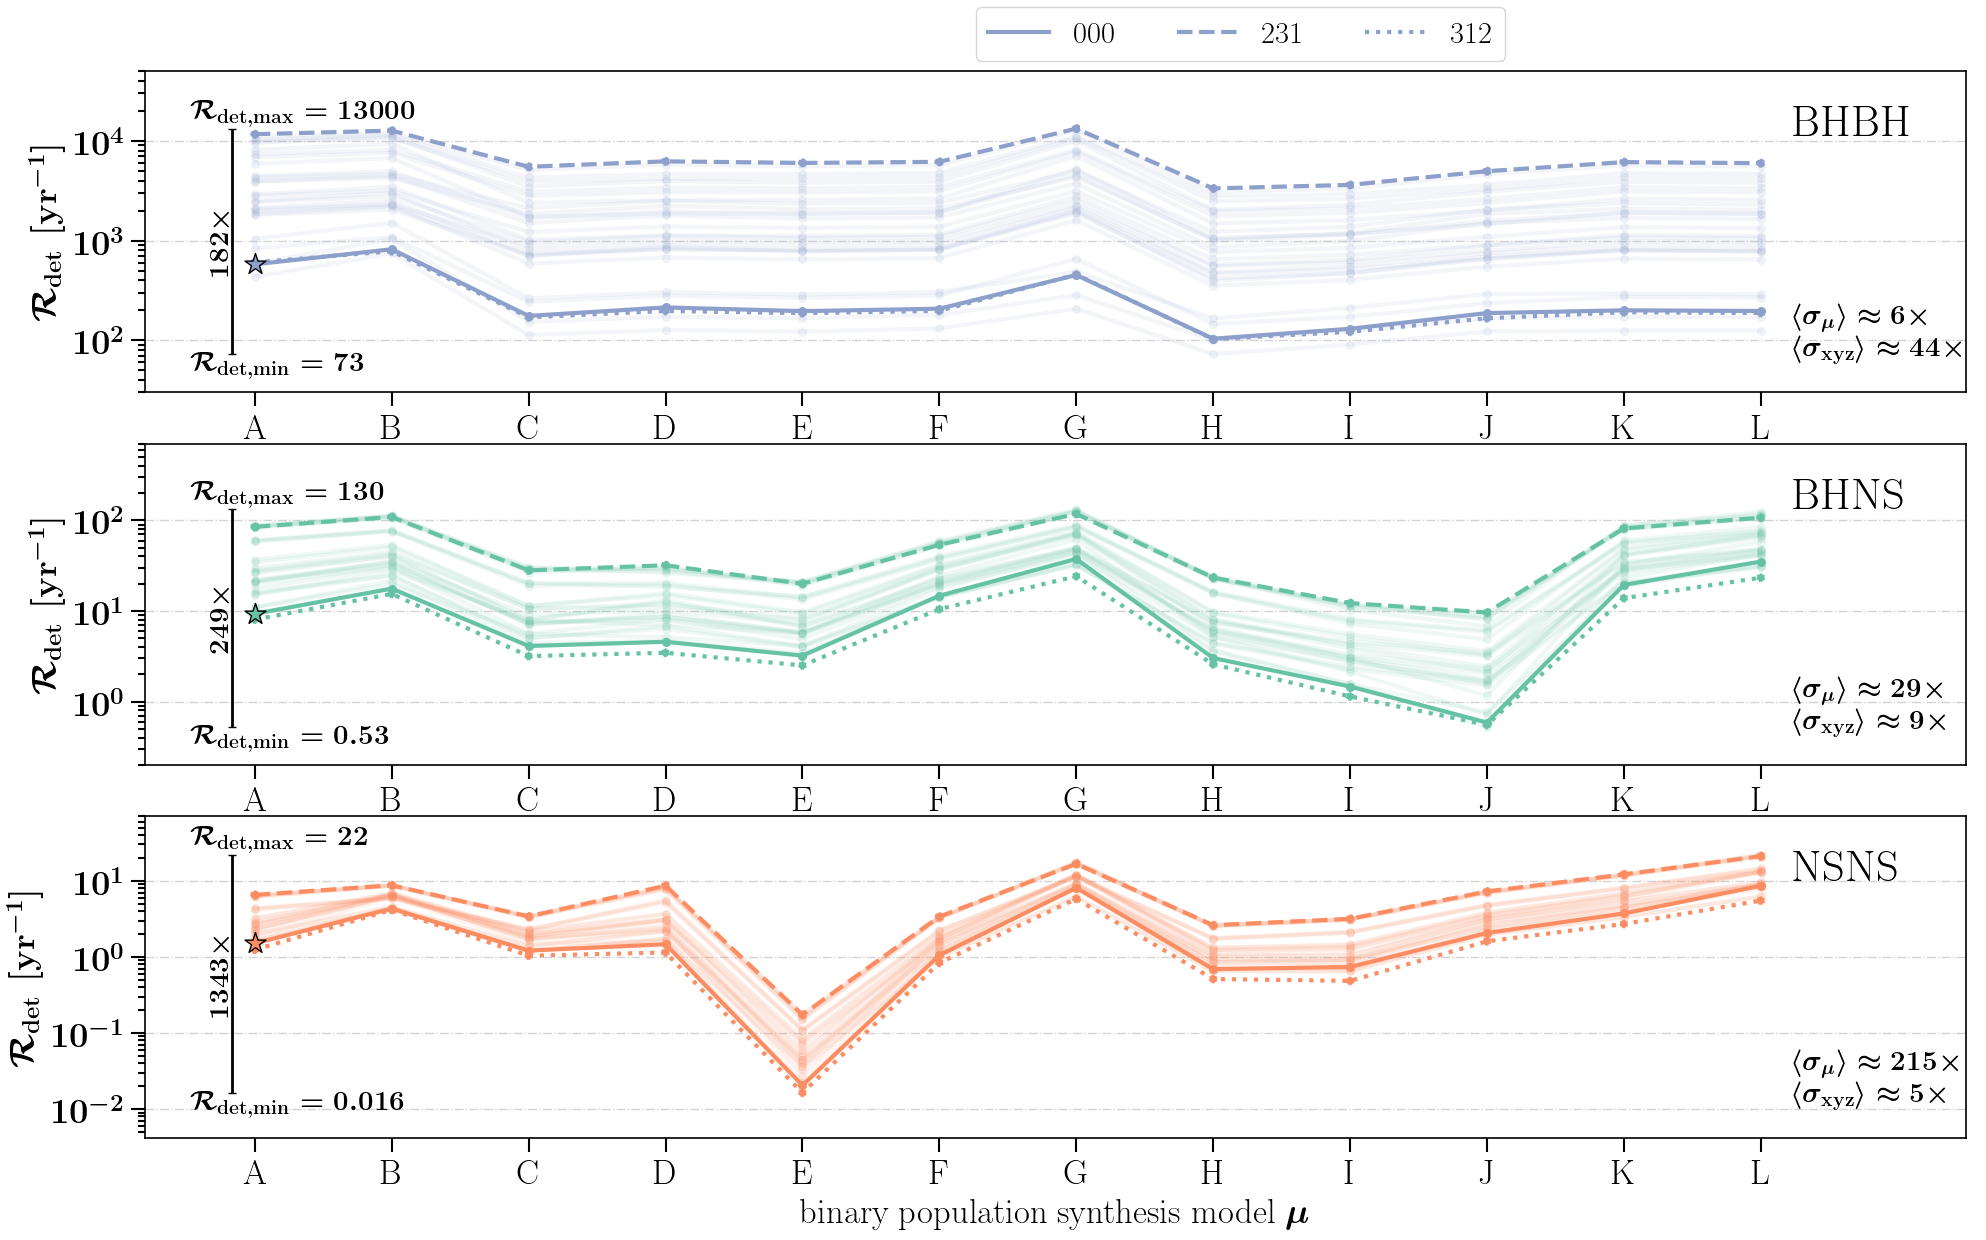
\includegraphics[width=1.0\textwidth]{../PlottingScripts/8_PredictedRates_BPS_and_MSSFR_variations/Rates_observed_AllDCO.png} 
%\includegraphics[width=1.0\textwidth]{../PlottingScripts/8_PredictedRates_BPS_and_MSSFR_variations/Rates_observed_analysisFiducialMSSFR_linestyleColouring.png} %
%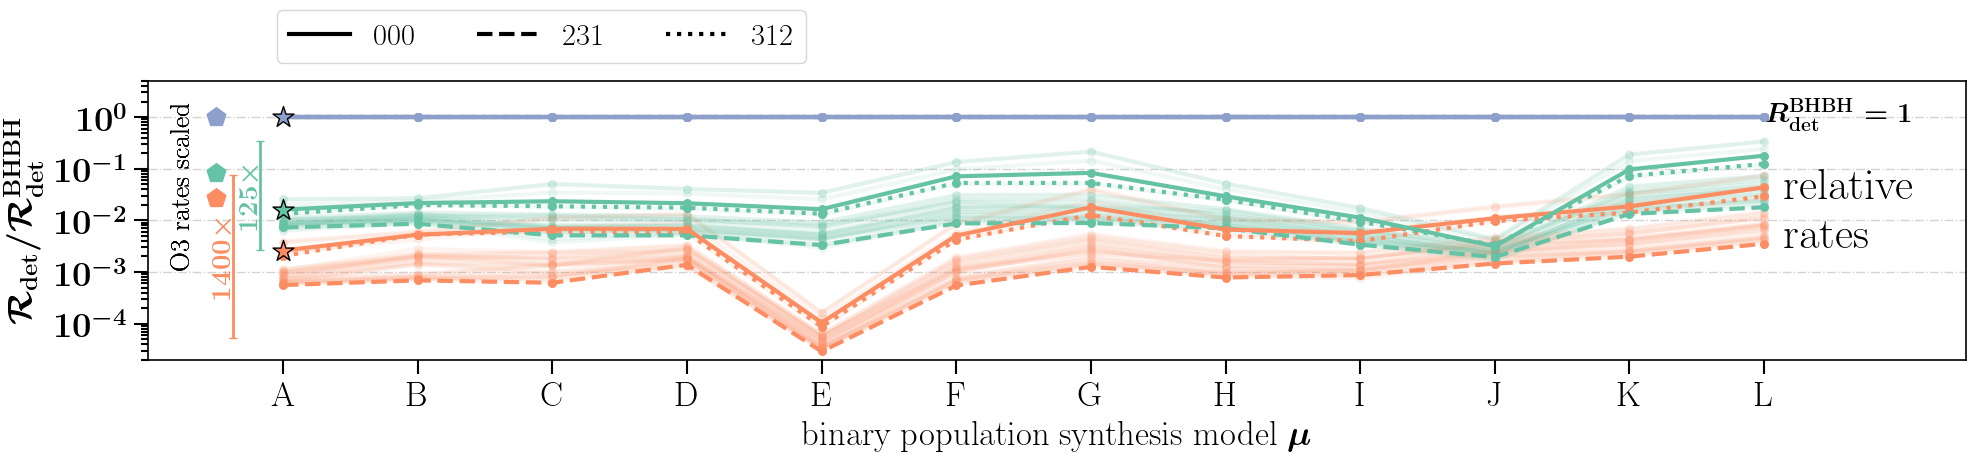
\includegraphics[width=1.0\textwidth]{../PlottingScripts/8_PredictedRates_BPS_and_MSSFR_variations/RatesRatios_observed.png} 
    \caption{Same as Figure~\ref{fig:IntrinsicRates} but showing the observed rates obtained by taking into account the \ac{GW} selection effects (Section~\ref{subsec:detection-probability}). We use the short-hand notation $\rate_{\rm{det}} \equiv \diff \Ndet / \diff \tdet$}%
    \label{fig:ObservedRatesBBHBNSBHNS}
\end{figure*}
%


The predicted detected merger rates for \ac{BHBH} and \ac{NSNS} mergers  are shown in Figure~\ref{fig:ObservedRatesBBHBNSBHNS}. 
Our fiducial model predicts detected rates of $\rate_{\rm{det}}^{\rm{BHBH}} \sim$\rateObsBHBH    \yearmin and $\rate_{\rm{det}}^{\rm{NSNS}} \sim$\rateObsNSNS   \yearmin for \ac{BHBH} and \ac{NSNS} respectively.  Considering the \Nmodels model variations we find predicted detected rates in $\rate_{\rm{det}}^{\rm{BHBH}}  \sim [\RateObservedAzeroBHBHmin, \RateObservedAzeroBHBHmax]\GpcminThree \yearmin$  and $\rate_{\rm{det}}^{\rm{NSNS}}  \sim [\RateObservedAzeroNSNSmin, \RateObservedAzeroNSNSmax]\GpcminThree \yearmin$, which ranges over  factors $\sim 180\times$ and $\sim 1340\times$ for \ac{BHBH} and \ac{NSNS} respectively. 


Figure~\ref{fig:IntrinsicRatesBBHBNSBHNS} shows that the optimistic \ac{CE} model (B) is an outlier and over-predicts  the observed \ac{BHBH} merger rate for all \ac{MSSFR} models. This model  allows binaries where a Hertzsprung gap donor star engages a \ac{CE} event to survive. This model also predicts   the highest \ac{BHBH} merger rates in other studies \citep[e.g.][]{2012ApJ...759...52D,2013ApJ...779...72D, 2015ApJ...806..263D, 2019MNRAS.490.3740N}. 

The other high predicted rates originate from models  G, K and L, which all favor lower (BH) SN natal kicks. These lower kicks result in  a smaller fraction of  binary systems disrupting during the \acp{SN} and to  higher yields of \bhnsSingle and \ac{NSNS} mergers whilst  the   \ac{BHBH} rates stay similar. These models therefore  also increase the ratio of \bhnsSingle and \ac{NSNS} mergers over \ac{BHBH} mergers.    


%
\begin{figure*}
    \centering
%    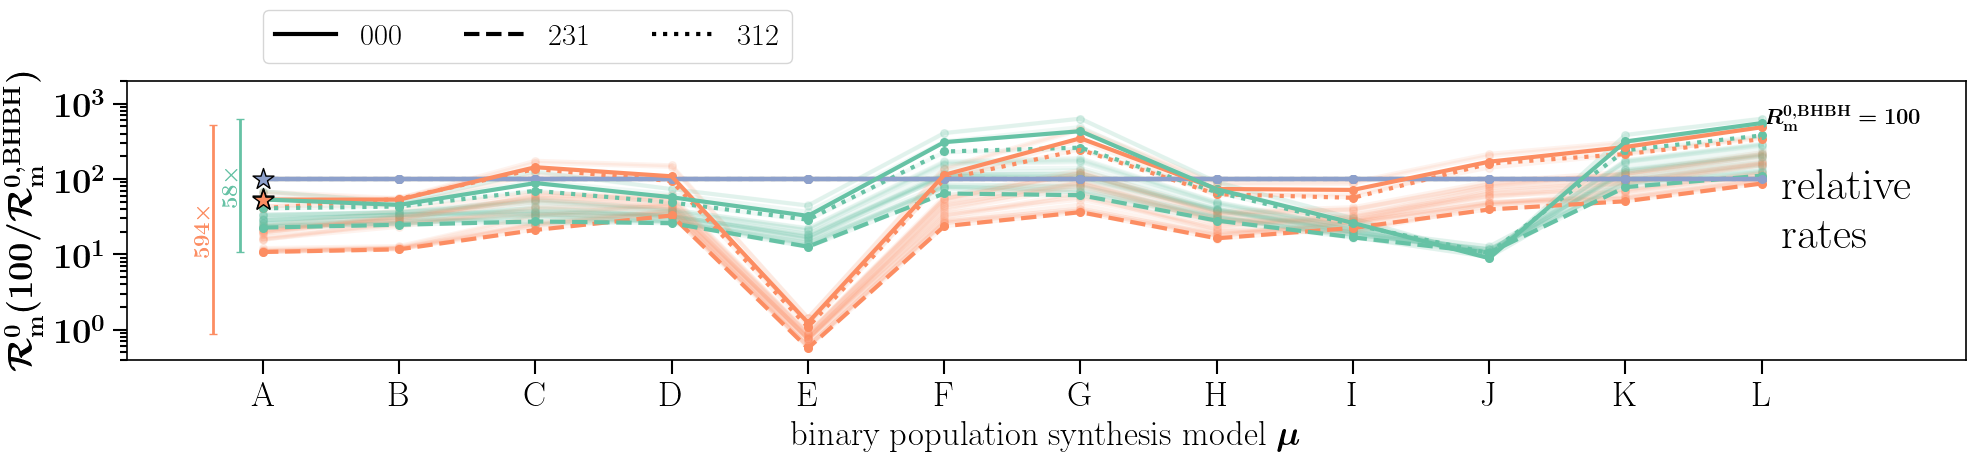
\includegraphics[width=1.0\textwidth]{../PlottingScripts/8_PredictedRates_BPS_and_MSSFR_variations/RatesRatios_intrinsic.png} 
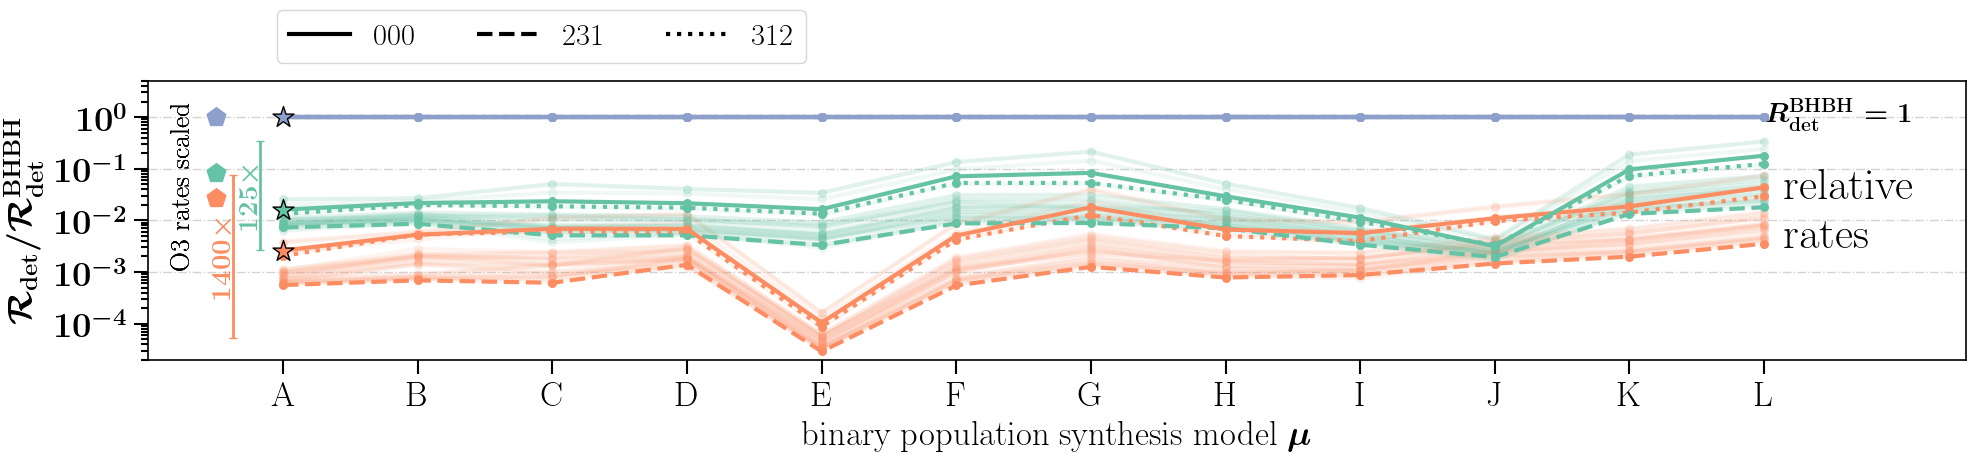
\includegraphics[width=1.0\textwidth]{../PlottingScripts/8_PredictedRates_BPS_and_MSSFR_variations/RatesRatios_observed.png} 
    \caption{Same as Figure~\ref{fig:IntrinsicRates} but  the observed rates that are obtained by taking into account the \ac{GW} selection effects (Section~\ref{subsec:detection-probability}). We use the short-hand notation $\rate_{\rm{det}} \equiv \diff \Ndet / \diff \tdet$. The rates are scaled relative to a fixed \ac{BHBH} rate of   $\rate_{\rm{det}}^{\rm{BHBH}}=100$\yearmin. Pentagon shapes show the O3 scaled number of alerts of each double compact object type. }%
    \label{fig:ObservedRatesRatiosBBHBNSBHNS}
\end{figure*}
%






The bottom panel  of Figure~\ref{fig:ObservedRatesBBHBNSBHNS} shows the relative merger rates when fixing the \ac{BHBH} rate to $\rate_{\rm{det}}^{\rm{BHBH}} = 100$\yearmin. We find that all our models predict a higher \bhnsSingle detection rate compared to \ac{NSNS} detections, except for the model where the mass transfer efficiency $\beta=0.75$ where \ac{NSNS} detections are more numerous.  This is in agreement to recent studies that also find higher \bhnsSingle merger rates compared to NSNS rates \citep{2019PhRvD.100f4060B}. However, other studies conclude that only in the optimistic CE simulation the \bhnsSingle merger detection rate surpasses the \ac{NSNS} rate  \citep{2015ApJ...806..263D}.
 In appendix~\ref{sec:app-predicted-rates-intrinsic} we show the relative intrinsic merger rates. In this case we find that more models predict similar or higher \ac{NSNS} rates compared to \bhnsSingle mergers but we also find several models with  higher intrinsic \bhnsSingle merger rates in contradiction with findings by e.g. \citet{2015ApJ...806..263D} who always find a higher intrinsic \ac{NSNS} rate compared to the \bhnsSingle merger rate.   %Compare with \citep{2019MNRAS.482.5012C}.

Section~\ref{sec:results-variations} showed that the \bhnsSingle rate decreases with increasing values for $\beta$ (models H, I, J). The \ac{NSNS} rate, on the other hand,  increases with increasing $\beta$. This leads that in particular $\beta$ is a variation that impacts the predicted ratios between \ac{NSNS} and \bhnsSingle mergers as can be seen in Figure~\ref{fig:ObservedRatesRatiosBBHBNSBHNS}.  Higher values for $\beta$ are preferred to match the \ac{NSNS} merger rate.  This is in agreement with recent findings from  \citet{2020arXiv200300195V} that suggest higher values for $\beta$ are preferred to match the observed Be-X-ray binary population. 
We conclude that comparing the relative rates between BHBH, \ac{NSNS} and \bhnsSingle mergers could therefore be especially informative  regarding models E, H, I, J, K and L. 


%: and the redshift dependent rate never surpasses, but only because the volume is larger). 

In the third observing run (O3) run by the gound-based \ac{GW} LVK network  there are about $\rate_{\rm{det}}^{\rm{O3}} \sim 50$  \ac{BHBH} detections expected.  If we scale the numbers from Figure~\ref{fig:ObservedRatesRatiosBBHBNSBHNS} to a \ac{BHBH} rate of 50 detection we find that our fiducial model predicts that for this number we expect about  $\sim 0.8 $ \bhnsSingle  and $0.1$ \ac{NSNS}  detections. Considering our \Nmodels model variations the predicted rates fall in the range $ \rate_{\rm{det}}^{\rm{O3}} \in  [0.14, 17]$ for \bhnsSingle and   $ \rate_{\rm{det}}^{\rm{O3}} \in  [0.0027, 3.8]$ per $50$ BHBHs. Where the rates on the higher end are from the models with no \ac{BH}- or low  SN natal kicks (models G, K and L).  
We also counted the number of double compact objects from the publicly available preliminary classification of \ac{GW} \href{http://chirp.sr.bham.ac.uk/alerts}{alerts} and found $37$ BHBH, $3$ \bhnsSingle and $1$ \ac{NSNS} mergers respectively, where we have not taken into account the mass gap events and only took into account events with a source origin probability classification of $\geq 90\%$. These numbers, scaled to a \ac{BHBH} rate of 100 events are shown with pentagon symbols in Figure~\ref{fig:ObservedRatesRatiosBBHBNSBHNS}. The current preliminary observed double compact object type ratios are on the high end regarding number of \bhnsSingle and \ac{NSNS} sources per BHBH and favor models G, K and L with low \ac{SN} kick magnitudes. Of course these preliminary number of \acp{DCO} are still uncertain. Once the new O3 catalog is out this will put tighter constrains on the possible models that can match the observed (relative) merger rates. 




%discuss relative rates.  Quote rates as found by first order classification. 
%

%\subsection{Uncertainty from binary population synthesis  on predicted rates}
%%








\subsection{Uncertainty from binary population synthesis and \ac{MSSFR} on the predicted rates}
%
Figure~\ref{fig:IntrinsicRatesBBHBNSBHNS} and \ref{fig:ObservedRatesBBHBNSBHNS} show that for \ac{NSNS} mergers the uncertainty from binary population synthesis models dominates  the scatter in the predicted rates compared to varying \ac{MSSFR},  similar to our findings for \bhnsSingle mergers as we showed in Section~\ref{sec:results-variations}. We find for \ac{NSNS}  $\langle \sigma_{\rm{\mu}}\rangle \approx 317, 215$ whereas   $\langle \sigma_{\rm{xyz}}\rangle \approx 5$ for both intrinsic and detected \ac{NSNS} rates.  
It can  be seen that especially model E is an outlier in the predicted rates for \ac{NSNS} mergers.  If we exclude the highest models we find instead $\langle \sigma_{\rm{\mu}}\rangle \approx 8,  9$  for intrinsic and observed \ac{NSNS} rates and   $\langle \sigma_{\rm{xyz}}\rangle \approx 4$ for both intrinsic and observed rates. 

 
For \ac{BHBH} mergers, on the other hand,  the \ac{MSSFR} variations dominate the predicted rates and we find $\langle \sigma_{\rm{\mu}}\rangle \approx 6$ whereas   $\langle \sigma_{\rm{xyz}}\rangle \approx 18$ and $44$.  %, whereas for 
We find that a subset of our chosen binary population synthesis model variations  such as models E, K and L do not drastically impact the \ac{BHBH} rate as these physics variations  mostly impact \acp{NS} and low mass \acp{BH}, which are only a small fraction of the \ac{BHBH} merger population. On the other hand, it is remarkable  that even changes in $\beta$ (models H, I, J) and  $\alpha_{\rm{CE}}$ (model C and D), barely impact the predicted \ac{BHBH} rates. Moreover, these model variations also do not significantly impact the shape of the \ac{BHBH} distributions as we  show later in this section.  We therefore suggest that \ac{BHBH} mergers are a good probe to constrain the \ac{MSSFR} models, whereas the \ac{NSNS} and \bhnsSingle merger rates can help constrain  the binary population synthesis models.

 


%
Compared to the intrinsic rates, the predicted detected rates are more sensitive to the \ac{MSSFR} prescriptions (especially for \ac{BHBH} mergers). This  is because \ac{GW} detectors are more sensitive to more massive double compact object mergers that typically form only at low metallicities. The yield of those mergers, that are detectable out to larger distances, depends strongly on the \ac{MSSFR} prescription. Therefore, typically $\langle \sigma_{\rm{\mu}}\rangle$ will be larger for the predicted detection  rates compared to the intrinsic rates. 
On the other hand, the scatter in predicted rates  from binary population synthesis variations $\langle \sigma_{\rm{xyz}}\rangle$ is stronger for the intrinsic rates compared to the detection weighted rates. This is because several model variations mostly impact lower mass remnants. Examples include model G, which assumes \acp{BH} receive no SN natal kicks and models K and L, which assume smaller SN kick magnitudes. 

%
%We show in Appendix~\ref{sec:app-BHBHandNSNS_CDF} that this is also  the case for the predicted \ac{NSNS} merger distributions. For \ac{BHBH} mergers, on the other hand,  the dominant factor affecting the shape of the distribution functions are the \ac{MSSFR} assumptions. 
%We  describe the shown \bhnsSingle parameters in more detail    below. 

\subsection{Comparison with the \ac{BHBH} and \ac{NSNS} distributions}
%
Similar to our results for \bhnsSingle we discuss in this section the shape of the  distribution functions for the   predicted \ac{BHBH} and \ac{NSNS} mergers characteristics.  These distributions are shown in figures~\ref{fig:ConfidenceINtervals_BHBH}--\ref{fig:PDF_NSNS}. 
%
\begin{figure*}
    \centering
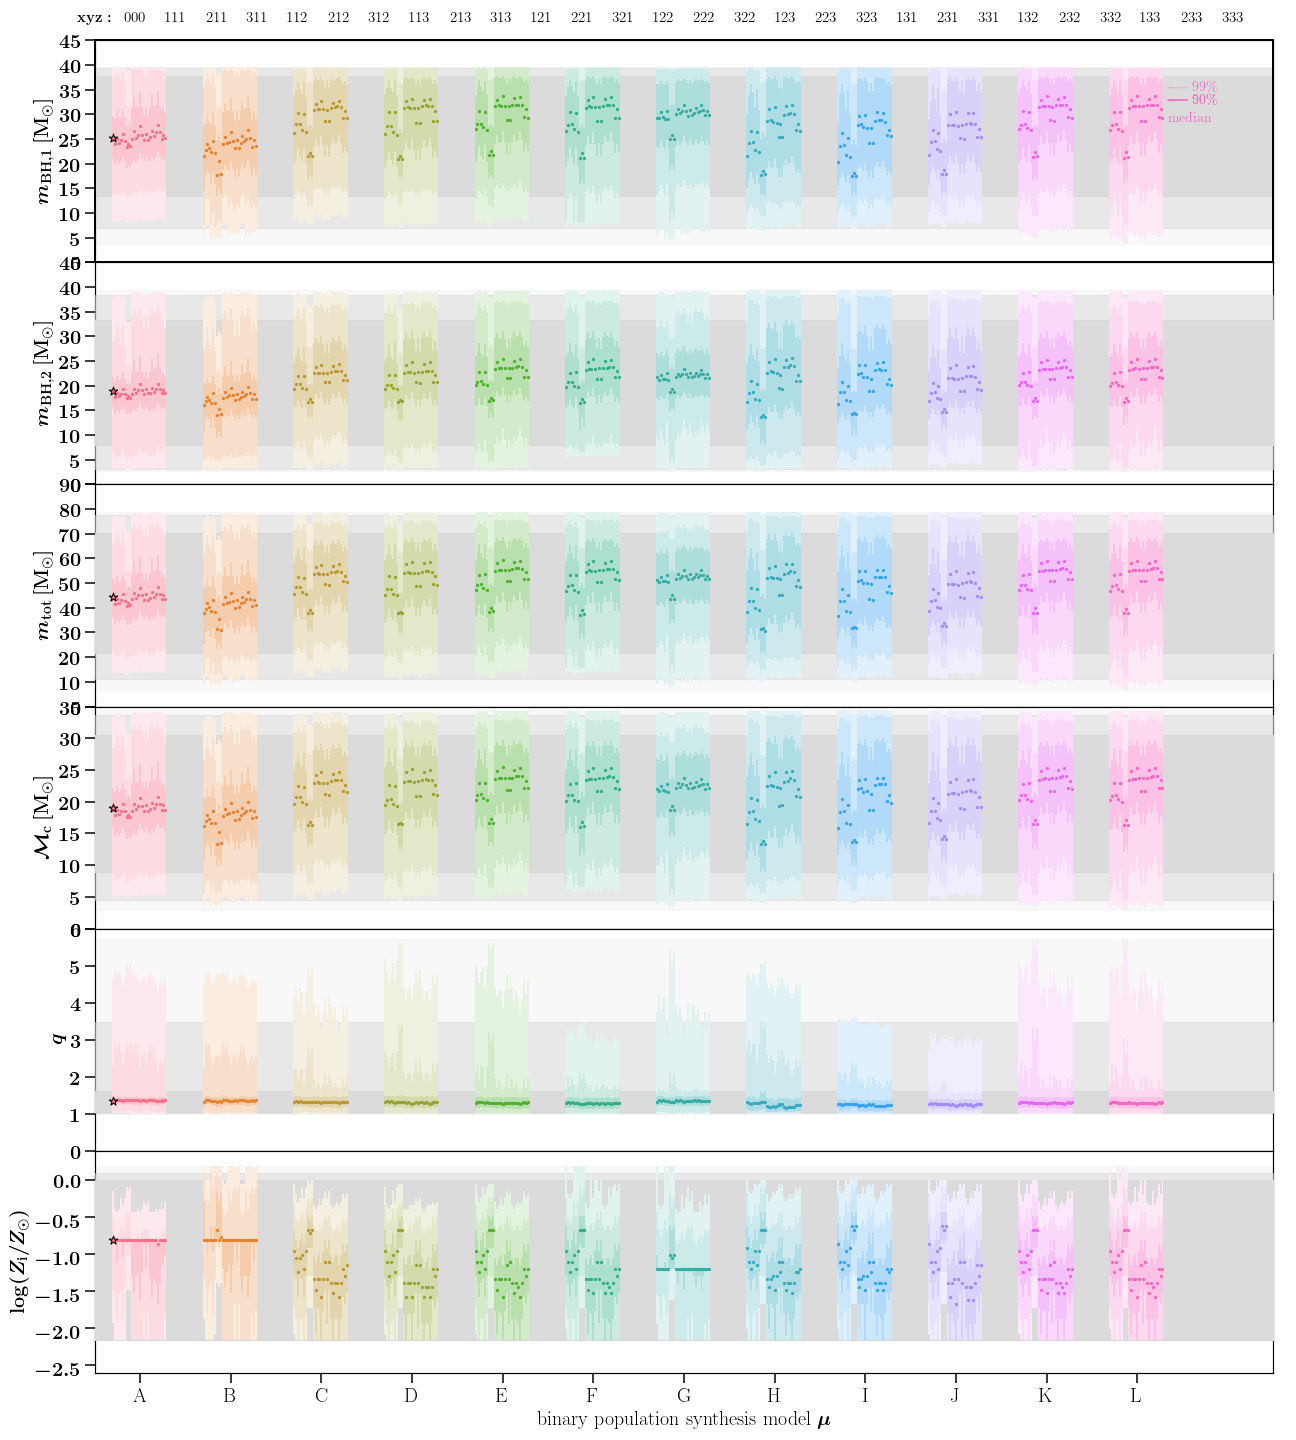
\includegraphics[width=1\textwidth]{../PlottingScripts/9_PredictedDistributions_BPS_and_MSSFR_variations/CDF_BPSandMSSFRvariations_Summary_BHBH_Z.pdf} %
\caption{Same as Figure~\ref{fig:ConfidenceINtervals_BHNS} but now for \ac{BHBH} mergers.}
    \label{fig:ConfidenceINtervals_BHBH}
\end{figure*}
%


\begin{figure*}
    \centering
%
\includegraphics[width=1\textwidth]{../PlottingScripts/9_PredictedDistributions_BPS_and_MSSFR_variations/PDF_BPSandMSSFRvariations_Summary_BHBH_Z.pdf} %
%
    \caption{Same as Figure~\ref{fig:PDF_BHNS}  for \ac{BHBH} mergers. The bar on the far right in each panel shows the distribution of the $90\%$ confidence intervals of the posterior samples of the observed BHBH from the O1 and O2 \ac{GW} run \citep{2019PhRvX...9c1040A}.  }
    %
    \label{fig:PDF_BHBH}
\end{figure*}
%


\subsubsection{BH mass distributions}
Although  \acp{BH} with  masses $\mbhf \lesssim 5\Msun$ are predicted to be common for \bhnsSingle mergers  this is not the case for \ac{BHBH} mergers, where we find that even when using the delayed SN remnant prescription  almost all models predict that less than 1$\%$ of the detected \ac{BHBH} mergers will contain a \ac{BH} with mass $\leq$5\Msun as can be seen in figures~\ref{fig:ConfidenceINtervals_BHBH} and~\ref{fig:PDF_BHBH}.  This indicates that even without forcing a lower \ac{BH} mass gap by construction with the rapid SN model,  \ac{BHBH} mergers with   \ac{BH} masses  $\leq$5\Msun  are predicted to be rarely detected with \ac{GW} observations. This indicates that  \bhnsSingle mergers are a better probe  compared to \ac{BHBH} mergers to explore the existence of the lower \ac{BH}  mass gap from  \ac{GW} observations. 

 Figure~\ref{fig:PDF_BHBH} shows that the most massive BH in the \ac{BHBH} merger typically has a mass in the range $ 12 \leq {\mbhf}_1/\Msun \leq  42$. The lack of \acp{BH} with masses $\gtrsim 40$\Msun\footnote{\ac{BH} formation is expected again above a helium core mass of $\sim 150$\,M$_\odot$ \citep{Woosley2002TheStars,Woosley2019TheLoss}} is because more massive \ac{BH} progenitors experience a pair-instability \ac{SN} where the \ac{SN} does not leave behind a \ac{BH} remnant as suggested from both observations \citep{2017ApJ...851L..25F,2018ApJ...856..173T,2019PhRvX...9c1040A, 2019PhRvD.100d3012W, 2019MNRAS.484.4216R,2019arXiv191209708G} and theory \citep{1964ApJS....9..201F,1967PhRvL..18..379B,2017ApJ...836..244W}.
  For some \ac{MSSFR} models there is a pile up of \acp{BH} with masses in $[35, 40]\Msun$ visible in  Figure~\ref{fig:PDF_BHBH}, which is a result from stars undergoing a pulsational pair-instability SN being mapped to similar \ac{BH} masses, something that also seems to be suggested from observations \citep{2018ApJ...856..173T,2019PhRvX...9c1040A}. The least massive BH in the \ac{BHBH} binary typically has masses $ 7 \leq {\mbhf}_2/\Msun \leq 32$. Compared to the \bhnsSingle mergers, 
the \acp{BH} in \ac{BHBH} mergers are typically  more massive. 




%Number of \ac{BHBH} mergers with low mass BHs is very dependent on model and MSSFR! So this will be a good prediction . 
%Only optimistic model makes \acp{BHBH} with mass smaller than 5. 
%
%Not so sensitive to even remnant mass function. 



\subsubsection{NS mass}
Figure \ref{fig:ConfidenceINtervals_NSNS} and~\ref{fig:PDF_NSNS} show that in almost all models the majority of \acp{NS} have masses around $\sim 1.3$\Msun. This is because in  the majority of \ac{NSNS} at least one of the stars experience either an \ac{ECSN} and/or \ac{USSN}, which  lead to \ac{NS} masses around 1.3\Msun  \citep[e.g.,][]{2017ApJ...846..170T,2018MNRAS.481.4009V}. 
Moreover, we find for \ac{NSNS} mergers that almost all models predict median \ac{NS} masses for both the most massive and least massive \ac{NS} below 1.8\Msun s and that \ac{NS} with masses $\geq 2\Msun$ are rare. The exception  is the binary population synthesis models with the unstable case BB mass transfer  (E) where the \ac{NS} typically are more massive.   This is because in this model the binaries that undergo case BB mass transfer merge before becoming a \ac{NSNS} system. Indicating that observing a lack of \ac{NSNS} mergers with the most massive \ac{NS} being below 1.4\Msun could suggest unstable case BB is a more representatitve model.  These observations are different from the \bhnsSingle mergers where Figure~\ref{fig:ConfidenceINtervals_BHNS} and~\ref{fig:PDF_BHNS} show that detecting systems with \acp{NS} masses above 1.8\Msun or 2\Msun is likely. 





%
%
%For the neutron stars we see that there are a few models that move around the nasses a lot , but MSSFR also does this (especially primary) . 


\subsubsection{Total mass}
%
Figure~\ref{fig:ConfidenceINtervals_BHBH} and ~\ref{fig:ConfidenceINtervals_NSNS} show that   for \ac{BHBH} and \ac{NSNS} mergers   $90\%$ of the total masses are predicted to lie in the ranges $\sim[11, 80]\Msun$ and  $\sim[2.5, 4.4]\Msun$ respectively. Only in models E and F the total \ac{NSNS} mass distribution are drastically different from the fiducial models. For \ac{BHBH} mergers, the total mass distributions are very similar except that some models slightly prefer more massive total masses. 

\subsubsection{Chirp mass}
%
The \ac{BHBH} and \ac{NSNS} mergers have for all \Nmodels model variations $90\%$ of the chirp masses lying in the ranges $\sim[5, 34]\Msun$ and $\sim[1.1, 2]\Msun$ respectively. This makes them very distinguishable from \bhnsSingle mergers, which 90$\%$ confidence interval typically lies in  $[2,5]\Msun$ We suggest that these distinguishable chirp mass population characteristics can be used to guide the choice of priors for population inference from \ac{GW} observations which will help distinguish between different double compact object types \citep[c.f.][]{2013ApJ...766L..14H,2015ApJ...807L..24L,2015MNRAS.450L..85M,2018ApJ...856..110Y}.




\subsubsection{Mass ratio}
For \ac{BHBH} mergers all our models remarkably predict a median \ac{BHBH} mass ratio around 1.4, indicating that if \ac{GW} observations have \ac{BHBH} mass ratios medians that are much higher that this might disfavor formation from isolated binary evolution. \ac{NSNS} mergers typically have mass ratios around $\qf \approx 1$. With the only exceptions model E and F where higher mass ratios are (also) preferred. 



\subsubsection{Metallicities}
%
The bottom panels of figures~\ref{fig:ConfidenceINtervals_BHBH}--\ref{fig:PDF_NSNS} show the shape of the birth metallicities of the BHBH and NSNS mergers. As expected, BHBH mergers typically originate from the lowest birth metallicities, namely typically $\log(\Zi) \sim [-2, 0.5]$, whereas NSNS mergers have the highest birth metallicities with  $\log(\Zi) \sim [-1, 0]$  also compared to \bhnsSingle mergers. The metallicity shifts to lower metallicities for BHBHs since the BHBH merger yield at those metallicities is much higher compared to higher metallicities.  The metallicities are also very dissimilar between the \ac{MSSFR} models, however birth metallicities are challenging to constrain from observations. 

\subsection{Uncertainty from binary population synthesis and \ac{MSSFR} on the predicted distribution functions}
%
Figure~\ref{fig:PDF_BHBH} shows that the normalized \ac{BHBH} distributions are relatively robust under changes in the binary population synthesis models and that the \ac{MSSFR} assumptions have a bigger impact on the shape of the BHBH distributions. 
Especially \ac{MSSFR} models 113, 213 and 313 are outliers  by predicting few \acp{BH} with masses in $30 \lesssim \mbhf / \Msun \lesssim 40$. The most right bar in the top panels of Figure~\ref{fig:PDF_BHBH} shows that these models are disfavored by the current \ac{GW} observations from GWTC-1.  We therefore predict that the \ac{GW} observed BHBH distributions will not be informative for binary population synthesis models and mostly informative in excluding \ac{MSSFR} models 113, 213 and 313. 

For NSNS mergers, the normalized distributions are also similar between most binary population synthesis models as can be seen in Figure~\ref{fig:PDF_NSNS}. Only model E and F are very dissimilar in the \ac{NS} mass distributions which also leads to distinguishable chirp mass and total mass distributions. The shaoe of the NSNS distributions is also similar under \ac{MSSFR} model variations. 

This is different compared to the shape of the \bhnsSingle distributions (Figure~\ref{fig:PDF_BHNS} where the shape of the distributions changes a lot with variations in binary population synthesis. We conclude, therefore, that among the \ac{DCO} merger types, especially the shape of the \bhnsSingle merger distributions will be informative to binary population synthesis model variations. 



%
\begin{figure*}
    \centering
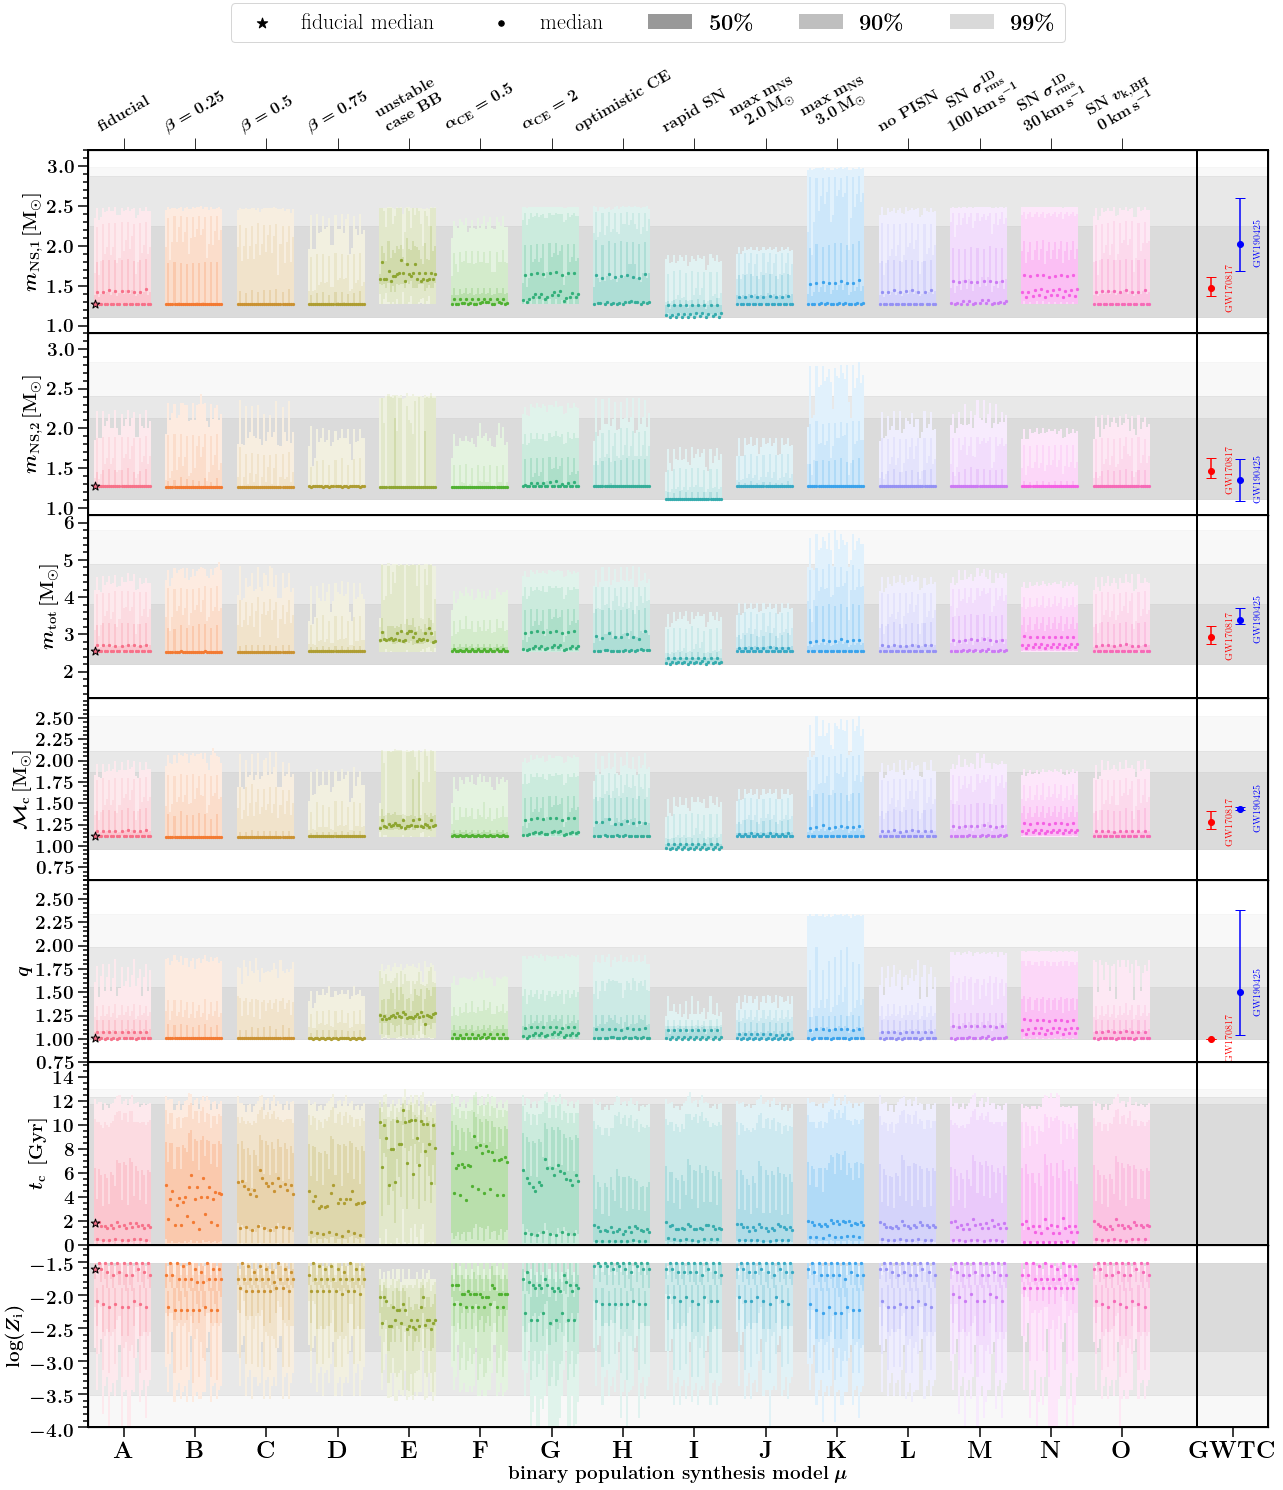
\includegraphics[width=1\textwidth]{../PlottingScripts/9_PredictedDistributions_BPS_and_MSSFR_variations/CDF_BPSandMSSFRvariations_Summary_NSNS_Z.pdf} 
\caption{Same as Figure~\ref{fig:ConfidenceINtervals_BHNS} but now for \ac{NSNS} mergers.}
    \label{fig:ConfidenceINtervals_NSNS}
\end{figure*}
%
\begin{figure*}
    \centering
%
\includegraphics[width=1\textwidth]{../PlottingScripts/9_PredictedDistributions_BPS_and_MSSFR_variations/PDF_BPSandMSSFRvariations_Summary_NSNS_Z.pdf} %
%
%
    \caption{Same as Figure~\ref{fig:PDF_BHNS} for \ac{NSNS} mergers. The bar on the far right in each panel shows the distribution of the $90\%$ confidence interval of the posterior samples of GW170817 from \citep{2019PhRvX...9c1040A}.   }
    %
    
%    \caption{Probability distribution functions for the predicted \bhnsSingle mergers  for the variations of MSSFR and binary population synthesis models studied in this paper. 
%    The distributions are weighted for the detection probability for a \ac{GW} network at design sensitivity. 
%    For each binary population synthesis model we show for each \ac{MSSFR} variation distribution function in a vertical bar. The color indicates the normalized probability of that bin.  It is visible that varying the binary population synthesis model $\mu$ dominantly affects the shape of the distribution and the most probable value for the characteristics of the detected \bhnsSingle mergers.  }
    %
    \label{fig:PDF_NSNS}
\end{figure*}
%




%%%%%%%%%%%%%%%%%%%%%%%%%%%%%%%%%
%%%%%%%%%%%%%%%%%%%%%%%%%%%%%%%%%%
%%%%%%%%%%%%%%%%%%%%%%%%%%%%%%%%%%

\section{Discussion }
\label{sec:discussion}






%We discuss prospects of identifying and characterizing black hole (BH) companions to normal stars on tight but detached orbits, using photometric data from the Transiting Exoplanet Survey (\url{https://arxiv.org/abs/1808.10856#})
%
%\url{https://arxiv.org/abs/1910.00822}
%We study the prospects of searching for black hole (BH) binary systems with a stellar-mass \ac{BH} and a non-compact visible companion, by utilizing the spectroscopic data of Large Sky Area Multi-Object Fiber Spectroscopic Telescope (LAMOST). they predict how many can be found. 
%
%
%BHNS CAN HELP FIND DETECT THE EOS  \url{https://arxiv.org/pdf/1103.3526.pdf}
%%Using recent post-Newtonian expressions and realistic equations of state to model these scenarios, we find that point-particle templates are sufficient for the detection of black hole-neutron star inspiralling binaries, with a loss of signals below 1% for both second and third-generation detectors. Such detections may be able to constrain particularly stiff equations of state, but will be unable to reveal the presence of a neutron star with a soft equation of state.


%The third observing run (O3) just finished and five alerts are already announced for \ac{GW} event candidates classified as a \bhnsSingle merger \citep[see the GCN alerts  by][]{GCNS190814bv,GCNS190910d,GCNS190923y, GCNS190930t,GCNS191205ah}.  

\subsection{Uncertainties beyond our models}

In this study we explored a total of \Nmodels models by varying \ac{MSSFR} and binary population synthesis assumptions. Below we discuss some of the main caveats of our study that should be further explored in future work. 

\subsubsection{SN remnant mass functions}
\label{subsec:discussion-delayed-vs-rapid-SN-remnant-mass}
One of the binary population synthesis models that resulted in drastic changes in the predicted  \bhnsSingle characteristics is model F that uses the \textit{rapid} SN prescription. Many binary population synthesis studies use the \textit{rapid} SN prescription instead of our default delayed SN remnant prescription. The {rapid} prescription assumes \ac{SN}  explosions occur within 250 ms (compared to longer timescales assumed for the delayed prescription) and reproduces, by construction,  the  lower remnant mass gap between NSs and BHs that is apparent from  X-ray binary observations 
\citep{1998ApJ...499..367B, 2010ApJ...725.1918O, 2011APS..APRH11002F} by a lack of BHs in the mass range between about the heaviest neutron stars  $\sim$ 2--3\Msun \citep{2016ARA&A..54..401O, 2017ApJ...850L..19M, 2019NatAs.tmp..439C,2019arXiv190801012T,2020arXiv200106102S} and  BHs of $\sim$ 4--7\Msun. 

%% \question{Should I discuss that  merging \ac{NS} product can fall in %\ac{BH} gap?} % \citep{2015ApJ...801...90P,2019ApJ...882L..24A}. 
%% 
	It is still under debate whether this lower \ac{BH} mass gap exists. Theoretical models of supernovae both predict a gap \citep{2014ApJ...785...28K,2015ApJ...801...90P} and no  gap (e.g. \citealt{1995ApJS..101..181W,2001ApJ...554..548F,2019arXiv191001641E, 2020arXiv200304320C})  in the mass distribution between \ac{NS} and \ac{BH} remnant masses. But see also \citet{2020MNRAS.491.2715B} who point out that it is very challenging to model remnant masses from supernovae explosions and that the compactness measure that is often used in these \ac{SN}  remnant mass studies is not a good metric for explodability of the supernova. 
	Moreover, \citet{2012ApJ...757...36K}   show evidence that the apparent observed mass gap from BHs in X-ray binaries could be caused by systematic offsets in the \ac{BH} mass measurements.  
	More recently, \citet{2019Sci...366..637T} found evidence for a $3.3_{-0.7}^{+2.8}$\Msun mass \ac{BH} observed in a non-interacting binary with a red giant, which is in addition of earlier observation of a speculated $\sim 2.44\pm0.27$\Msun \ac{BH} \citep{2002A&A...392..909C,2010AAS...21541905R,2011arXiv1107.1537D}. 
	In addition,  \citet{2016MNRAS.458.3012W,2019arXiv190407789W} studied microlensing events of BHs based on  observations from OGLE-III and Gaia data release 2.  
	They find evidence for a continuous distribution of stellar remnant masses and disfavor a mass gap between NSs and BHs (unless BHs receive natal-kicks above 20-80\kms).   
	In addition, the LIGO-Virgo Collaboration reported at the time of writing three candidate \ac{GW} events in their O3 observation run with at least one component in the lower mass gap \citep{GCNS190924h,GCNS190930s,GCNSS200115j}.	
%	We therefore conclude that based on the above, there is no clear evidence that the rapid remnant mass prescription  should be preferred in population synthesis simulations. 
	Moreover, \citet{2018MNRAS.481.4009V} show that the delayed prescription better matches the observed distribution of masses of Galactic double \ac{NS} systems. 
We  therefore decided to adopt the delayed remnant mass prescription as the fiducial model. 
	
In practice, both the delayed and rapid \ac{SN} model might not represent the \ac{SN} remnant mass distribution and future work should therefore explore other alternatives. Examples include the \citet{2016MNRAS.460..742M} prescription used in \citet{2018MNRAS.481.4009V} and the more probabilistic remnant mass function from \floor{Mueller and Mandel in prep.}

\subsubsection{ECSN prescription}
Another important assumption that can change the final masses of the \bhnsSingle distributions which needs to be further explored in the future is the helium core mass limit that leads to \ac{ECSN}. Several values are used in the literature. E.g., recently \citet{2004ApJ...612.1044P} argued  that helium core ranges of 1.4--2.5\Msun are more realistic and \citet{2015ApJ...801...32A} and Vinciguerra. (in prep.) show a different electron-capture range (resp. 2--2.5\Msun and 1.85--2.25\Msun, where the latter is based on \citealt{2008ApJS..174..223B}) could better reproduce observations of neutron stars. 
Future work should explore how changing this limit affects the predicted rate and characteristics of \bhnsSingle mergers.  



%
%\subsection{Mass transfer stability}
%\floor{discuss Coen his paper}
%
%











%
\subsubsection{MSSFR}
There are several uncertainties within \ac{MSSFR} that we have not explored in this study. 
First, all our \ac{MSSFR} models are described by simply parameterized MZR, \ac{SFR}  and \ac{GSMF} functions that do not take into account the likely dependencies between the prescriptions \citep[e.g.][]{2020arXiv200106025K}. 
Second, the relations are often based on a limited set of observations that do not explore the large range of redshifts where the observed \ac{GW} mergers might origin from \citep[e.g.][]{2020ApJ...893..111L}. 
In addition, one of the main uncertainties in \ac{MSSFR} is the definition of the solar metallicity value.  In this study we follow  \citet{2019MNRAS.490.3740N} by defining the solar metallicity as $Z_{\odot}=0.0142$ and the solar oxygen abundance as $\log_{10}[O/H]+12 = 8.69$ based on \citet{2009ARA&A..47..481A}. However, the assumptions for the solar metallicity and solar oxygen abundance vary across observations and theoretical studies of the MZR, \ac{GSMF} and \ac{SFR}  relations \citep[e.g.,][]{2019MNRAS.488.5300C}.  \citet{2019MNRAS.490.3740N} show that the variation of the relation between solar metallicity and the scaling with the solar oxygen abundance can add a  factor $3\times$ in the predicted rates for \ac{BHBH} mergers. 


%Extremely cool MZ paper: 
%\url{https://arxiv.org/pdf/1910.00597.pdf}
%The Mass-Metallicity and the Fundamental Metallicity Relation revisited on a fully Te-based abundance scale for galaxies [GA] The relationships between stellar mass, gas-phase metallicity and star formation rate (i.e. the Mass-Metallicity, MZR, and the Fundamental Metallcity Relation, FMR) in the local Universe are revisited by fully anchoring the metallicity determination for SDSS galaxies on the Te abundance scale defined exploiting the strong-line metallicity calibrations presented in Curti et al. (2017)



%\href{https://arxiv.org/abs/2001.06025}{SFR-mass relation paper note} 

%\url{https://arxiv.org/abs/1910.04168} discusses that the SF and galaxy mass is not well known for redshifts higher than 2. and helps improving this. 


\subsubsection{Initial conditions}
For our models we now assumed fixed initial distributions such as for the initial masses and separation distributions. In practice these distributions are uncertain \citep[e.g.,][]{2018Sci...359...69S}. Moreover, there is also evidence that some might  be metallicity or redshift dependent \citep[e.g.,][]{2018ApJ...855...20G}, which is not taken into account in this study. 

Studies have suggested that for a given binary population synthesis model a change in initial conditions mostly alters the rate of double compact objects but  does not affect drastically the merger properties. \citep{2015ApJ...814...58D}.
Future work should explore how uncertainties from initial conditions changes the predicted rates and distributions for BHNS mergers. 



%IMF slope might be more shallow 
%
%
%from de Mink and belczynski 2015: There are relatively few formation channels for double compact object mergers. For a given model of evolution, these formation channels originate from a rather narrow volume of initial parameter space (the formation volume). Change of initial conditions alters the number of the progenitor binaries in the formation volume, but has very little effect on the binary merger properties. This insensitivity is not just connected to the specific initial conditions considered here, but is of more fundamental nature. It is a robust result that has also been found in connection to other compact object binaries. For example by Kalogera $\&$ Webbink (1998) in the context of low-mass X-ray binaries, and see also Belczynski et al. (2002).
%
%


%
%
%\subsubsection{remnant mass function }
%
%\subsubsection{additional uncertainties MSSFR:}
%from unknown solar metallicity
%%\subsection{Galactic BH--NS }
%%
%%
%%
%
%\subsection{BH--MSP systems}
%
%
%\subsection{standard candals}
%The observed drop-off in the abundance of  45Msun black holes can be used to probe cosmic expansion by making binary black hole mergers``standardizable`` (Farr et al. 2019). 
%
%
%\subsection{Arxiv discussion}
%% The precise determinations of stellar mass at $\sim$1% provide important constraints on stellar evolution models. Accurate parallax measurements can also serve as independent benchmarks for the next Gaia data release. Aims. We aim at measuring the masses and distance of binary systems with a precision level better than 1% using a fully geometrical and empirical method. http://arxiv.org/abs/1910.03393
%
%
%
%
%
%
%\section{stuff from papers:}
%
%%\subsection{Simulation set up}
%%\begin{itemize}
%%	\item one model
%%	\item 30 different metallicities
%%	\item 1 million binaries per metalicity
%%	\item pop synth + \ac{MSSFR} 
%%	\item how do we select BH--NS and NS--BH
%%\end{itemize}
%%
%%
%
%\subsection{IMF}
%From \url{https://arxiv.org/pdf/1910.01126.pdf}
%
%The present--day generally accepted IMF[11] can thus be well represented by the canonical two-part power-law function with$ x = 0.3$ for $0.1 < $m/Msun $< 0.5$ and $x = 1.3 $for $0.5 leq$ m/Msun $< 150$. This IMF shape was confirmed[12]
%
%Recent observations have uncovered a dependency of the IMF on metallicity and density[15], [16], and infrared surveys have shown stars to form in long and thin molecular cloud filaments[17], challenging the gravo-turbulent theory of the IMF.

%
%\subsection{wind prescription}
%we use wind mass loss rates by \citet{2000A&A...362..295V,2001A&A...369..574V}. Where the line-driven wind loss scales with metallicity as $Z^{m}$ with $m\approx 0.69$, which is found to be  in agreement with  observations \citep[][]{2007A&A...473..603M}. Although the amount of mass loss is uncertain \cite{2014ARA&A..52..487S, 2017A&A...603A.118R} -  see also a review by \citep{2014ARA&A..52..487S} for more information.
%\subsection{case BB MT}
%The starting point of all these calculations (tight systems containing a naked helium star and a \ac{NS} with orbital period, Porb $< 2$ days) is a continuation of the expected outcome of common envelope (CE) evolution in high-mass X-ray binaries. Of particular interest is mass transfer by Roche-lobe overflow (RLO) initiated by the helium star expansion after core helium exhaustion (so-called Case BB RLO).
%%Tauris 2015
%\subsection{USSN}
%we now don't allow USSN for case BB onto a \ac{BH} 
%
%\textbf{tauris2015}
%I found this in Tauris2015, when they calculate the USSN rate : 
%"On the other hand, we have to include similar systems producing black hole–NS binaries and also add the number of systems (a factor of a few) which were disrupted as a consequence of the dynamical effects of the second  \ac{SN} explosion, and are therefore not contributing to the estimated merger rates quoted above."
%Which seems to suggest that Tauris thinks that USSN are formed in BH-NS binaries, if the \ac{BH} forms first (and thus the USSN star is the pre-NS)  %
%%https://iopscience.iop.org/article/10.1088/2041-8205/778/2/L23/pdf
%The explosion of ultra-stripped stars in close binaries can lead to ejecta masses $\leq0.1 M_{\odot}$ and may explain some of the recent discoveries of weak and fast optical transients.
%
%
%The total amount of helium in this envelope is 0.033Msun. The ultra-stripped nature of our model is achieved because the helium star is forced to lose (almost) its entire envelope in a very tight orbit where a \ac{NS} can fit in.
%%https://watermark.silverchair.com/stv990.pdf?token=AQECAHi208BE49Ooan9kkhW_Ercy7Dm3ZL_9Cf3qfKAc485ysgAAAl4wggJaBgkqhkiG9w0BBwagggJLMIICRwIBADCCAkAGCSqGSIb3DQEHATAeBglghkgBZQMEAS4wEQQMDnT5Wc8OYSqJBrW0AgEQgIICERaGRzgIOiqhB_3Emkt0HOzs_QrLS9snb99E0wHmM41oca9I5z4tNYkEpiPlg7Z8xDdOD31N7qwvGiSUOH5vGJxEKPEK5WHAe8-6NIYc70InoJ_ApOZUU_jW8SQu0ukAUlOaCyzyUGWPJkVTHgEb5SSRHq03kw-6TIQHVarRQo5EzejN1fXlOZgAJ6claZL7gPji9M6WwEZm4e_6Cxzczm9ekynhHy05_H7mC9sVcejPbp-33_yzxCpL6kkOwEvXwbOV4_WC6F_Effjet5FWIj3oh948r37v1NHVuk2K6GGO7A10h9eExvTZzXDL06G2qzRqj2WOKmWKgB1iloWJdhECyoIrjVYPV8gKgsw9SvztCxX7VULHAw42BG4derqsGNmT-bFc1LIbDygwQ8rS3Uuxd-0DDf71J-d5dsxfpf78xl1mpU-uxJaGqbm--h0pAQpOnX_Y2i9k1pIriaxyi4KwVRptO-WqrKYSxySBMZOGHz_SqBoCWjMYruBoVVaK5iTye1X3vZiN-XzjDRGdAZti1IlogcghQzpf9WB0vfRUhWvWqfRMQ0dtlX2t0r9l8-YOVtpAF7SoKLIKioJzWNIM1mONUpVVdWD5z4QJhfe7n72Vlx3yxBZ-J4eFpOxhFfn4rIj4H63Nb2C0CCNcCqYfMpqsZXu_3iLlatfVL2-6DrA1Z3kPAqn4Cq3tFNFbKag
%
%
%In other words, ultra-stripped SNe are exploding stars which contain envelope masses $\leq 0.2$M and having a compact star companion. The compact nature of their companion allows for extreme stripping in a tight binary, in some cases yielding an envelope mass $\leq 0.008$Msun %10.1093/mnras/stv990
%%Ultra-stripped supernovae: progenitors and fate 
%
%It has recently been demonstrated (Tauris et al. 2013, 2015)
%that close--orbit DNS systems (i.e., those that are tight enough to merge within a Hubble time due to GWs) must form via ultra-stripped SNe when the last star explodes. The reason being that Case BB RLO, i.e., mass transfer via Roche-lobe overflow from a naked helium star in the post-HMXB/post-CE system, causes the \ac{NS} to significantly strip its evolved helium star companion almost to a naked metal core prior to its explosion. This has an important effect on the number and properties of surviving DNS systems-in particular, in terms of their kinematic properties-as we shall discuss rigorously in more
%%Tauris DNS 
%
%
%% from Combine 
%If the exploding star forms the second-born compact star of the binary, it undergoes an ultra-stripped  \ac{SN} (Tauris et al. 2013, 2015; Suwa et al. 2015; Moriya et al. 2017) because of severe mass stripping by the nearby compact object, leaving an almost naked metal core at the time of the explosion. For such ultra-stripped SNe we apply w1Drms $= 30$ km /s,
%in accordance with the many double \ac{NS} systems observed with small eccentricities of $e <
%\sim 0.2$ (Tauris et al. 2017).\\
%
%
%\textbf{COSMIC has it:}
%\url{https://cosmic-popsynth.github.io/docs/latest/inifile/index.html}
%Reduces kicks according to the sigma div selection for ultra-stripped supernovae which happen whenever a He-star undergoes a \ac{CE} with a compact companion
% 
%
%\subsection{Optimistic vs Pessimistic}
%\textbf{Vigna--Gomez 2018}
%We allow donor stars which engage into a \ac{CE} phase during hydrogen shell burning (HG) to survive the event and expel the common envelope if allowed by the energy condition. This assumption is labeled ``optimistic``CE in the literature (Dominik et al. 2012), while the alternative, ``pessimistic`` CE, always leads to a merger for HG donors.
%
%\textbf{Dominik2012:}
%The impact of the \ac{CE} outcome on binary populations
%depends strongly on the evolutionary stage of the donor, as first discussed in Belczynski et al. (2007). The Standard model does not allow for \ac{CE} events with HG donors. These stars are not
%expected to possess a clear core-envelope structure (Ivanova and Taam 2004), thus making it difficult for them to eject their outer layers during the \ac{CE} phase. In our Standard model all \ac{CE} events with HG donors lead to a prompt merger before a DCO binary is formed, regardless of the aforementioned energy balance. The
%%http://dx.doi.org/10.1088/0004-637X/806/2/263
%
%
%\textbf{Mapelli}
%Finally, we have revised the treatment of Hertzsprung gap (HG) donors in CE: HG donors are assumed to always merge with their companions if they enter a \ac{CE} phase. This is justified by the fact that HG stars have not yet developed a steep density gradient between core and envelope, and allows us to match the merger rate of BHBs (Mapelli et al. 2017) inferred from LIGO--Virgo observations (Abbott et al. 2016a).
%%arXiv:1806.00001v1
%
%\textbf{Wiktorowics and Belczynksi}
%%https://arxiv.org/pdf/1907.11431.pdf
%We assume that non-DCO mergers occur in the follow- ing situations:
%(1) failed envelope ejection during a \ac{CE} event (e.g. Justham et al. 2014),
%(2) donor in a \ac{CE} phase haven’t developed a clear boundary between core and the envelope (e.g. MS and HG donors; Ivanova and Taam 2004),\\
%
%\textbf{Olejak Belczynski }
%2.3. Hertzsprung gap stars in common envelope
%We calculated two \ac{CE} models (marked as A and B) which represent different scenarios for binary system with Hertzsprung gap star (HG) as a donor in the \ac{CE} phase. In model B we assume that all of such binary systems merge during \ac{CE} and possibly create a single BH. In model A we let such a system to survive \ac{CE} phase on the energy balance calculations (Webbink 1984). Currently it is not well known which scenario operates (Ivanova and Taam (2004)).
%
%%We present population synthesis statistical estimates of the cur- rent Milky Way black hole population properties. We used the most current version of the StarTrack code with standard physics (Sec. 2) and processed the data with the new star formation rates and metallicity distribution model of our Galaxy, based on theo- retical models and observations. We show results for two mod- els: A and B, which correspond to different scenarios of a \ac{CE} phase (Sec. 2.3). We find that:
%%1) At the current moment the Milky Way (disk+bulge+halo) contains about 1.6 × 108 single black holes with average mass 13 M⊙ and 9.3 × 106 black holes in binary systems with average mass 19 M⊙.
%%2) There are three main formation channels of single BHs: ∼ 35% are remnants of massive single star evolution, ∼ 40% formed in binary systems merger, ∼ 25% of single BHs orig- inate from disrupted binary systems during black hole/neutron star formation.
%%3) The most massive black hole in simulation comes from old, low in metal environment of Galactic halo. It formed in MS-He stars coalescence and its mass is as large as ∼ 130 M⊙.
%%4) Black holes in binary systems constitute ∼ 10 % of the whole Galactic \ac{BH} population. Most of BHs in binary systems are in \ac{BHBH} configuration. The fraction of black hole binaries with non compact companion is small, about 0.3 % of all Galactic BHs.
%%-We estimate how double compact object systems merger rates (BHBH, BH-NS and NSNS) have changed along with the Galaxy star formation. Current Galactic merger rates depend on model and they are estimated at ∼ 81/3 Myr−1 for BHBH, ∼ 9/1 Myr−1 for BH-NS and ∼ 59/14 Myr−1 for \ac{NSNS} systems.
%%5) We constrain that only ∼ 0.005 % of total Galactic halo mass (including dark matter) could be hidden in the form of stellar ori- gin BHs which are not detectable by current observational sur- veys
%%6) Only ∼ 5 % of single BHs and 0.001 % of binary BHs have enough high velocities to escape from Galactic potential.
%%On Figure 6 we show how the total number of BHs formed in the Milky Way have been changing since the Milky Way forma- tion till current time with assumed star formation rates and star metallicity distribution (Sec.2.5) for two evolutionary models A and B.
%\subsection{DELAYED FRYER}
%1) The defaults are in some sense meaningless. They are intended as something like a best guess, but we will always want to demonstrate how variations away from this default affect our conclusions. For this reason I don't think it really matters which one we choose as default.
%2) Rapid reproduces NS-BH mass gap. By construction, it does this. However since it is not clear whether this gap is real, or due to some selection effect, I do not find this a compelling reason to prefer it 
%3) The rapid prescription does not reproduce the observed DNS masses. As we showed in Alejandro's paper, the rapid prescription (combined with other COMPAS defaults) does a miserable job of reproducing the observed DNS masses. Delayed did a bit better.
%4) For massive BHs formed through complete fallback, the two prescriptions are the same, so again there is no real reason to prefer one over the other
%From Alejandros paper:
%In fact, the  RAPID  \ac{SN} mechanism (01) allows for low-mass NSs which would be difficult to differentiate from NS–white dwarf binaries; there are several non-confirmed DNSs or poorly constrained DNS masses in the region favoured by the “rapid” mechanism (01) (Ozel et al. 2010; Ozel $\&$ Freire 2016). On the other hand, the seven existing well-constrained mass measurements in this study are inconsistent with the predictions of the fiducial model (01) at a $>$ 4sigma level. None of these seven measurements fall below a chirp mass of 1.1 Msun, while 83 per cent of DNSs in the fiducial model have lower chirp masses. This suggests that the RAPID mechanism under-predicts the amount of collapsed mass for the lowest-mass NSs for both ECSNe and USSNe.
%
%Fryer rapid, on the other hand, is hardcoded to have a maximum of 2.0 solar masses. So, if you use the rapid Fryer, it will make no different.\\
%
%
%\textbf{ERTL and Woosley 2019}
%ERTL and Woosley \url{1910.01641} find : Lower mass black holes exist though, on down to the maximum neutron star mass. There is no unpopulated ``gap``.
%
% The most obvious difference of the helium-star explosions compared to the single-star models of Sukhbold et al. (2016) (see also Appendix A) is the greater number of cases with significant fallback.
% 
% These fill in a ``gap`` in the remnant mass distribution that might have existed between gravitational masses of about 2 to 6Msun. Most cases where black holes are formed by fallback are associated with progenitors that explode very late (texp$\sim$ 2 s) at the time when the infalling point with entropy per baryon 6.0 reaches the shock. 
% Such cases form massive proto-neutron stars (see sect 4.1) that explode with relatively low energies (about 1--4 $\cdot 10^{50}$ erg) and eject no iron-group material (in the absence of mixing). The fallback includes much of the progenitor mass. Typically 2--3Msun are still ejected in models with standard mass loss, but only 1--1.5Msun for the most massive helium stars with enhanced mass loss
%
%The smaller mass black holes are made by fallback after the initial launch of a successful shock. The lowest mass black holes made in any models for the W18 central engine were 2.29, 2.31, and 2.56Msun, which came from stars with initial helium star masses of 22.0, 21.25, and 22.25Msun, respectively. The
%
%although \url{http://arxiv.org/abs/1909.04152} show that explodability and 1d and 2d simulations like above are not the way to do it. True nature of remnant is unknown. 
%


%\section{EM counterparts}
%
%\subsection{BH spins}
%Finally, as has been noted by other authors, these results may point to the simple fact that binary black hole component spins are intrinsically small (Farr et al. 2017; Tiwari et al. 2018; Wysocki et al. 2019). (from \href{https://arxiv.org/pdf/2001.06051.pdf}{this paper})
%
%\href{http://arxiv.org/abs/2001.04474}{detections of binary-black-hole mergers revealed the ubiquity of massive black holes (Abbott et al. 2019), some of which may be spinning rapidly (Venumadhav et al. 2019).}
%
%\subsection{GRB and kick}
%Mikes paper \url{https://arxiv.org/abs/1910.03598}
%\subsection{BH--NS vs \ac{NSNS} kilonova}
%
%\url{https://arxiv.org/pdf/1210.6549.pdf}
%We find that collisions between neutron stars and
%stellar mass black holes, which, due to their larger capture radius, should dominate over \ac{NSNS} collisions by a factor of $\sim$ 5 (Lee et al. 2010), eject significantly larger amounts of matter, typically $\sim$0.15 \Msun. Unless equation of state or relativistic gravity effects dramatically modify these results, the overall rate of compact object collisions should therefore be seriously constrained, otherwise r-process elements would be substantially overproduced.
%
%\url{https://arxiv.org/pdf/1611.09822.pdf}
%We find that the more promising dynamic ejecta models from \ac{NSNS} mergers reach K-band peak magnitudes in excess of -15 (model N5 with a mass ratio close to the observed \ac{NSNS} binary J0453+1559; see right panel of Figure 9), while the brightest NSBH dynamic ejecta model reaches values beyond -16. The wind models with parameters inspired by neutrino-driven winds from an NSNS-merger peak below -13, while models mimicking unbound torus matter (Just et al. 2015; Wu et al. 2016) reach peak values of -14 and - with only slightly increased mass and velocity parameters – they can reach close to -16 (Figure 11).
%
%
%\url{https://arxiv.org/pdf/1910.01617.pdf}
% For BH--NS mergers, in the (possibly rare) subset of low-mass/high--spin BHs which disrupt the \ac{NS} well outside the horizon, the red kilonova will be more luminous, and extend to higher velocities, than in the \ac{NSNS} case due to the greater quantity of tidal tail ejecta. As in the prompt collapse of a NSNS, the blue component-if present-will arise from the relatively low-velocity disk wind and thus could be blocked for equatorial viewers by the lanthanide-rich tidal tail ejecta
%
%\label{sec:bhns-EjectedMass}
%\begin{itemize}
%	\item detection of GW170817 has confirmed that double compact object mergers can produce r-process enrichment
%	\item two known UFD galaxies are observed to be r-process enriched  which can be explained with one merger event 
%	\item Safarzadeh et al. showed that this could be by highly eccentric or short separation born \ac{NSNS} binaries
%	\item However, literature has shown that BH--NS are also r-process enrichment sources 
%	\item such systems are more massive and will have smaller $v_{\rm{sys}}$ and $v_{\rm{kick, reduced}}$ and can therefore play an important role for UFD galaxies.  
%	\item here we study the possible role of  BH--NS in enrichment of UFD galaxies.
%\end{itemize}
%
%
%In the case of a \ac{NSNS} merger, tidal disruption during the inspiral phase leaves behind an accretion torus surrounding the merged object (either a \ac{NS} or a BH), unless the two NSs have identical masses (Shibata et al. 2006; Rezzolla et al. 2010; Giacomazzo et al. 2013; Hotokezaka et al. 2013; Kiuchi et al. 2014; Ruiz et al. 2016; Radice et al. 2016).
%An energetic engine can be driven by rapid accretion onto to the remnant object and/or by dipole radiation losses if the remnant is an hypermassive or stable \ac{NS} (Giacomazzo & Perna 2013; Ciolfi et al. 2017). Growth and collimation of magnetic fields during the merger, as well as neutrino losses, are then believed to power a relativistic outflow. Dissipation within the expanding flow, and later interaction of the flow with the interstellar medium, gives rise to radiation that spans a wide window in the electromagnetic spectrum, from high-energy γ-rays down to the radio. This basic scenario has been observationally confirmed with the recent event GW170817/GRB170817A (Abbott et al. 2017). Mergers
%Mergers of BH-NS binaries (always resulting in a \ac{BH} as
%the resulting compact remnant) are expected to be accom- panied by the formation of an hyperaccreting disk only if the mass ratio between the \ac{BH} and \ac{NS} does not exceed the value ∼ 3−5, with the precise value depending on the equa- tion of state of the \ac{NS} and the \ac{BH} spin (Pannarale et al. 2011; Foucart 2012; Foucart et al. 2018). (see e.g. Bartos et al. 2013 for a review)

%Additionally note that, independently of the post-
%merger EM signal, a fraction on the order of a few ×10−3 of the GW sources is expected to be accompanied by an SN-type precursor (Michaely & Perets 2018). This is due to the fact that the distribution of the delay time between the last  \ac{SN} explosion and the binary merger has a non-negligible tail of ultra-short times, on the order of 1-100 yr (see also (Dominik et al. 2012)).
%\subsubsection{UFD galaxy properties}
%\begin{itemize}
%	\item UFD enriched candidates
%	\item virial radius of those galaxies
%	\item masses of UFD
%	\item we therefore take the following values for the properties of the UFD: 
%\end{itemize}
%
%
%\subsubsection{Definition of a candidate BH--NS}
%we take a similar definition as in 
%
%
%
%
%\subsubsection{stay in Halo}
%\begin{itemize}
%	\item we consider 2 type of halo`s with 1.3 kpc and 4.6 kpc halo
%	\item escape velocities are X and Y 
%	\item masses are X and Y 
%\end{itemize}
%
%\subsubsection{what fraction of BH--NS systems produces r-proces enrichment}
%\label{subsec:EMcounterparts}
%%
%%REF suggest that similar to \ac{NSNS} mergers, BH--NS mergers can be a r-process site. 
%Simulations show that, in the case of a BH--NS merger, the \ac{NS} can either (i) plunge into the black hole or (ii) tidally disrupt, dependent on the mass ratio, spins and \ac{NS} equation of state (EOS). If the \ac{NS} is dirsupted, a fraction of the material can be ejected 
%
% most of the matter will fall onto the black hole within a few subseconds. However a small fraction of the material can stay bound and form a disk and a fraction of the matter might be unbound and ejected during the merger. In this case the BH--NS constitutes an r-process site that can enrich 
%
%
%\begin{itemize}
%	\item it is thought that some cases \ac{NS} plunges into the \ac{BH} in a BH--NS merger
%	\item this is dependent on spin, EOS, mass ratio of BH--NS system
%	\item we use Foucart +2018 to determine the ejecta mass. This is given by the following equation. it uses the following assumptions 
%	\item we plot the dependency on spin (and how much mass is ejected) 
%	\item show plot Mass \ac{BH} vs (see Foucart) 
%\end{itemize}
%
%
%%\begin{figure*}
%%	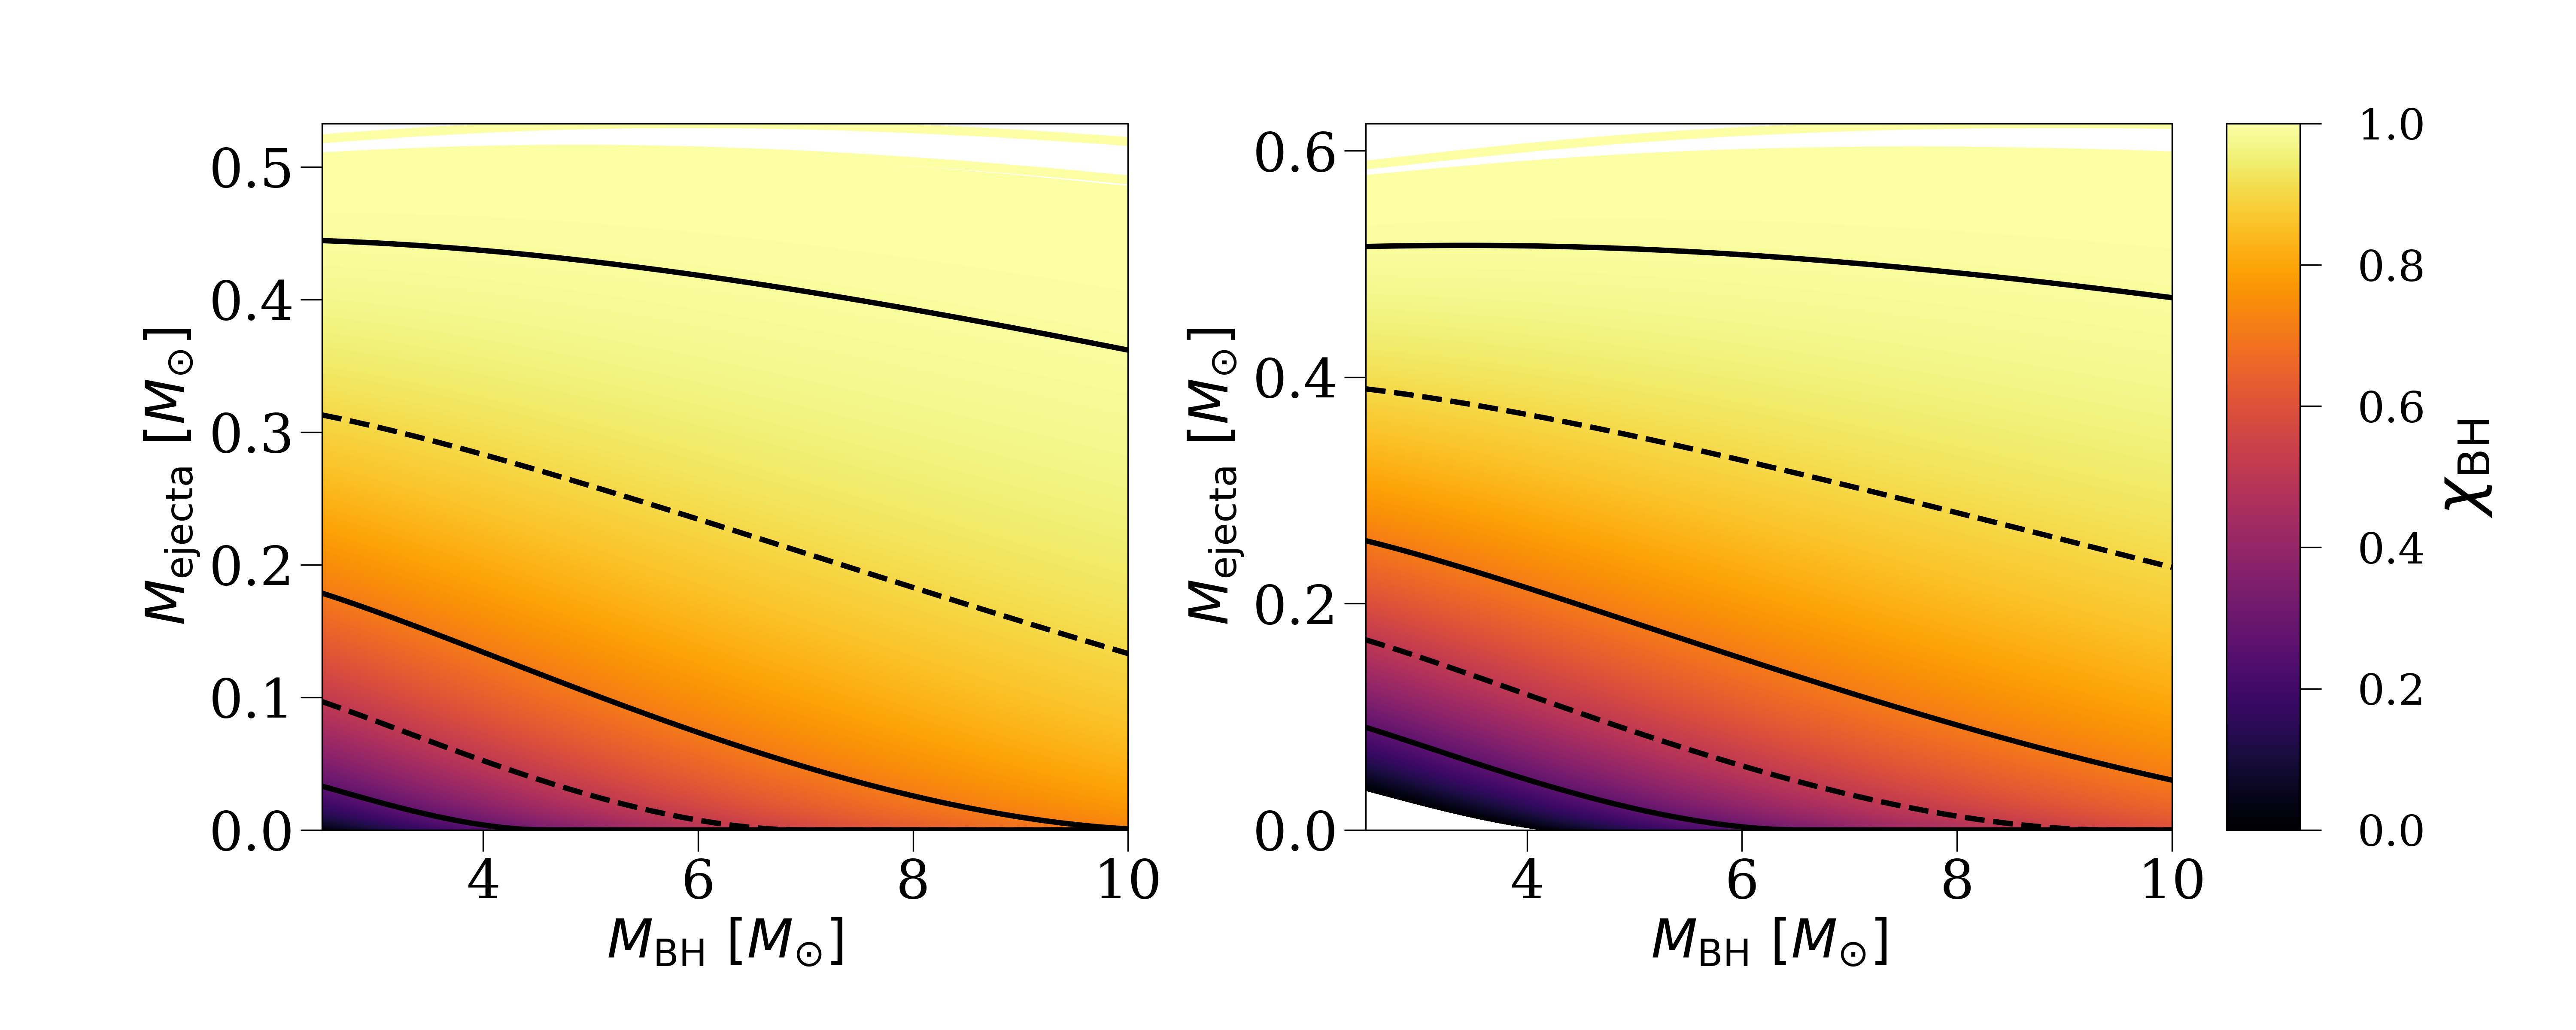
\includegraphics[width=1\textwidth]{../PlottingScripts/imagesUFDandRatios/PredictedMej.png} %CPUVsUncertaintySingleTogether.pdf}
%%    \caption{}
%%%    The number of binaries found of the target population  $N_{\mathrm{T}}$ as a function of the total number of binaries $N_{\text{binaries}}$ sampled for the traditional sampling method (gray dashed line) and the sampling method presented in this study (solid colored line). The four different panels show the simulations for each of the four target subpopulations. In each panel the duration of the exploratory phase is shown with a hashed gray area.  In the background the standard Poisson fractional uncertainties  of $0.3, 1$ and $3\%$ are shown with a dashed line.  } 
%%    \label{fig:PredictedMej}
%%\end{figure*}
%%%
%
%
%
%\subsubsection{Role of BH--NS compared to \ac{NSNS} }
%\begin{itemize}
%	\item drake formula for rate of candidate 
%\end{itemize}
%
%\begin{equation}
%	\mathcal{R}_{\rm{candidates}} \approx \mathcal{R}_{\rm{merger}} \times f_{\rm{merges \ in \ halo}} \times f_{\rm{enriches}}
%\end{equation}
%
%
%%
%
%\subsubsection{rates of BH--NS candidates versus \ac{NSNS} candidates }
%Table~\ref{tab:summary-simulations} summarizes the results from our binary population synthesis simulations focusing on the candidate systems that can enrich UFD galaxies from the different models simulated in this paper. The weight quoted in the table represent the number of candidate systems expected to form out of $10^6$ binaries drawn from the birth distributions as described in Section~\ref{sec:method}. 
%The weight  of BH--NS candidates in our \fiducial model is \fexplTwo, \EffExplTwo and   \EffRefTwo  for respectively assuming a black hole spin of $ \chi_{\rm{bh}} = 1, \chi_{\rm{bh}} = 0.5, $ and $\chi_{\rm{bh}} = 0$. 
%%The first column shows the physical models simulated in this work, where we show the  the different BH--NS simulations and the results for our \fiducial \ac{NSNS} simulation for comparison.
%%The 2nd -- 4th columns show the total weight of the candidate systems in our simulation, which are defined as all the BH--NS or \ac{NSNS} mergers that merge well within a halo with mass of $M \approx 10^9 \, M_{\odot}$ $(10^8 \, M_{\odot})$, with$ r_{\rm{vir}} \approx 4.6 \rm{kpc}$ $( \approx 1.3 \rm{kpc})$ with redshift $ z = 6 $ ( $ z =  10 $). Where the different columns represent different assumptions for the spin of the black hole in the $BH--NS$ binary of $\chi_{\rm{bh}} = 1, \chi_{\rm{bh}} = 0.5, $ and $\chi_{\rm{bh}} = 0$. 
% 
% 
 %%% TABLE
%\begin{table*} %{Summary of Adaptive Importance Sampling method results \\}
%\centering
%\label{tab:comparison2}
%\begin{tabular}{|l|c|c|c|c|c|c|c|}
%\hline
%\hline
%  Model		    &   weight candidates   &   weight   candidates  		&    weight  candidates  &  weight  all    & Fraction &   $\#$ candates /   	\\
%    &    $\chi_{\rm{bh}}=1$   &  $\chi_{\rm{bh}}=0.5$ 		&   $\chi_{\rm{bh}}=0$   &    &  &    $\#$ all mergers  	\\ \hline 
%NSNS \fiducial    &  \fexplOne  & \EffExplOne  & \EffRefOne & \NxMCOne   & \NxAISOne & \gainOne  \\ \hline
%BH--NS  \fiducial   &  \fexplTwo  & \EffExplTwo  & \EffRefTwo & \NxMCTwo   & \NxAISTwo & \gainTwo  \\ %\hline
%BH--NS   $Z=0.002$   &  \fexplThree  & \EffExplThree & \EffRefThree & \NxMCThree   & \NxAISThree & \gainThree  \\ %\hline
%BH--NS reduced kick  &  \fexplFour  & \EffExplFour  & \EffRefFour & \NxMCFour   & \NxAISFour & \gainFour  \\
% BH--NS $\alpha =0.1$       &  \fexplFive  & \EffExplFive  & \EffRefFive & \NxMCFive   & \NxAISFive & \gainFive  \\
%  BH--NS $\alpha =10$  &  \fexplSix  & \EffExplSix  & \EffRefSix & \NxMCSix   & \NxAISSix & \gainSix  \\ 
%  BH--NS Fryer \texttt{RAPID}  &  \fexplSeven & \EffExplSeven  & \EffRefSeven & \NxMCSeven   & \NxAISSeven & \gainSeven  \\  
% \hline
%\end{tabular}
%\caption{The total weight (i.e. number) of double compact objects formed out of $10^6$ binaries simulated in each model. The total weight is derived from combining the probability of occuring of each binary in the simulation and equals `the number of binaries out of the total simulation`.  A description of the models is given in Section \ref{subsec:method-COMPASmodel}.  The 2nd to 4th column give the total weight of double compact objects that merges well within the virial radius of  a halo with mass $10^9 M_{\odot} \ (r_{\rm{vir}}   = 4.6 \, \rm{kpc})$ at $z \approx 6$. In parenthesis the total weight of the systems is shown that merge within a halo of mass   $10^8 M_{\odot} $ $ (r_{\rm{vir}}   = 1.3 \, \rm{kpc})$ at $z \approx 10$. The fifth column shows the total weight of all double compact object systems that merge within a Hubble time, and the sixth column shows the fraction  of all double compact object mergers that is a candidate system. The last column shows the total number of binaries out of $10^6$ that evolved to a candidate and to all double compact object systems.  }
%\label{tab:summary-simulations}
%\end{table*} 



%
%\subsection{BH--Pulsars}
%Detecting  \bhnsSingle systems with a pulsar would provide a unique laboratory to test general relativity and alternative theories of gravity \citep{Wex:1998wt,KRAMER2004993, 2014arXiv1402.5594W} and will enable high precision  measurements of the  properties of black holes    \citep{1975ApJ...198L..27B,1975SvAL....1....2B}. However, to date, no BH--pulsar system has been observed through radio observations. This might not entirely be surprising as several studies estimate that the ratio between  \ac{BH}--pulsar  and \ac{NSNS} in our Milky Way is about one in a 1000 \citep{2005ApJ...628..343P}. Currently there are about 20 \ac{NSNS} known \citep[e.g.][]{tauris2017formation,2019ApJ...876...18F}.  A more in depth study of predictions for BH--pulsars from COMPAS is done in \floor{Debatri in prep.}


%Similar to  \citep{2016A&A...596A..58K} we estimate that 







%\https://arxiv.org/abs/1804.06014
%We have performed population synthesis calculation on the formation of binaries containing a black hole (BH) and a neutron star (NS) in the Galactic disk. Some of important input parameters, especially for the treatment of common envelope evolution, are updated in the calculation. We have discussed the uncertainties from the star formation rate of the Galaxy and the velocity distribution of \ac{NS} kicks on the birthrate (∼0.6−13Myr−1) of BH/NS binaries. From incident BH/NS binaries, by modelling the orbital evolution duo to \ac{GW} radiation and the \ac{NS} evolution as radio pulsars, we obtain the distributions of the observable parameters such as the orbital period, eccentricity and pulse period of the BH/pulsar binaries. We estimate that there may be ∼3−80 BH/pulsar binaries in the Galactic disk and around 10\% of them could be detected by the Five-hundred-meter Aperture Spherical radio Telescope.
%
%\subsection{Variations}
%\label{subsec:bhns-discussion-variations}
%
%\href{https://arxiv.org/pdf/1708.07885.pdf}{compare with variations this paper}


%\subsection{learn about \ac{BH} mass function}
%%
%see \href{https://arxiv.org/pdf/2002.02981.pdf}{this paper}

%\subsection{Rates ratios}
%From Dominik2012
%One exception is the Optimistic \ac{CE} model, in which the merger rate per unit volume is large enough (while still being lower than for \ac{NSNS} systems at all redshifts) that BH--NS detection rates are larger than \ac{NSNS} rates because they are observed farther (see Table 1 and Figure 6).

%%
%\subsection{relativeRates}
%%
%

%\subsection{BH--NS}
%might be needed for early r-process enrichment \href{https://arxiv.org/pdf/1601.06966.pdf} t%202020-02-06%2022.23.12.png?dl=0

% UNDO DO THIS FOR UFD galaxy rates plots
%
%\begin{figure*}
%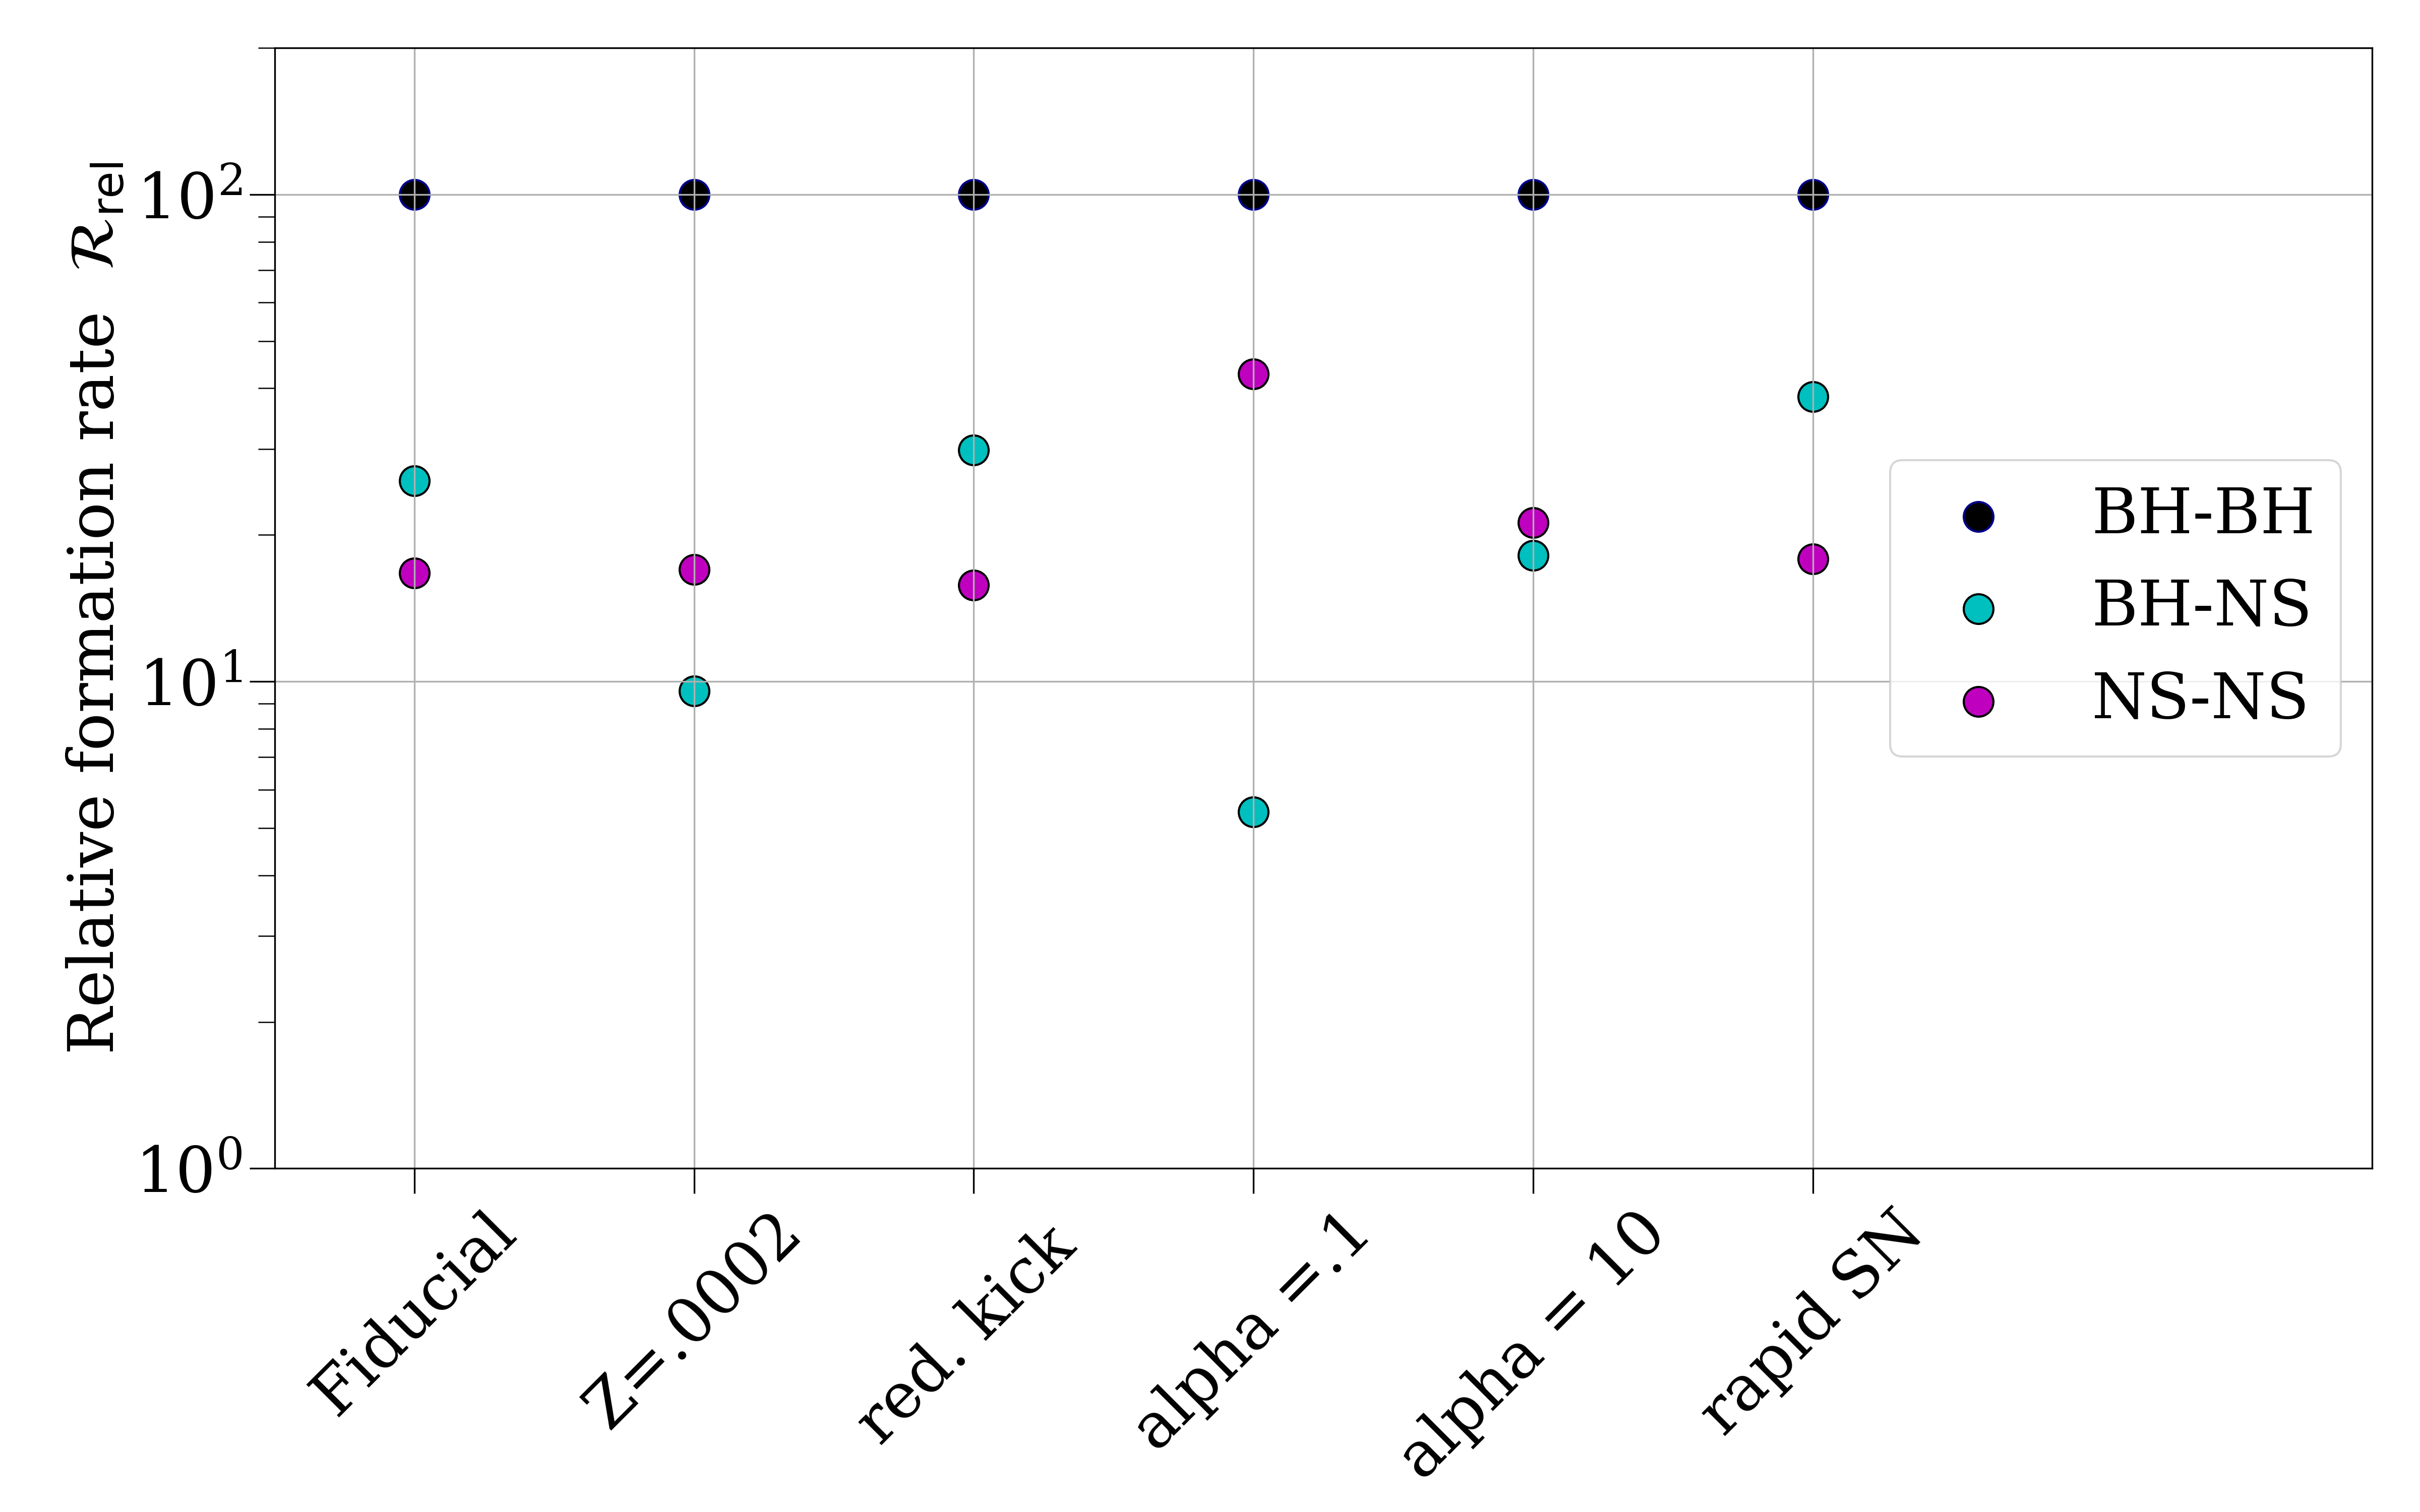
\includegraphics[width=.8\textwidth]{../PlottingScripts/imagesUFDandRatios/relativerates_formation.png}
%   \caption{ }
%  \label{fig:BHNS_DCO_j}
%\end{figure*}
%%
%
%%
%\begin{figure*}
%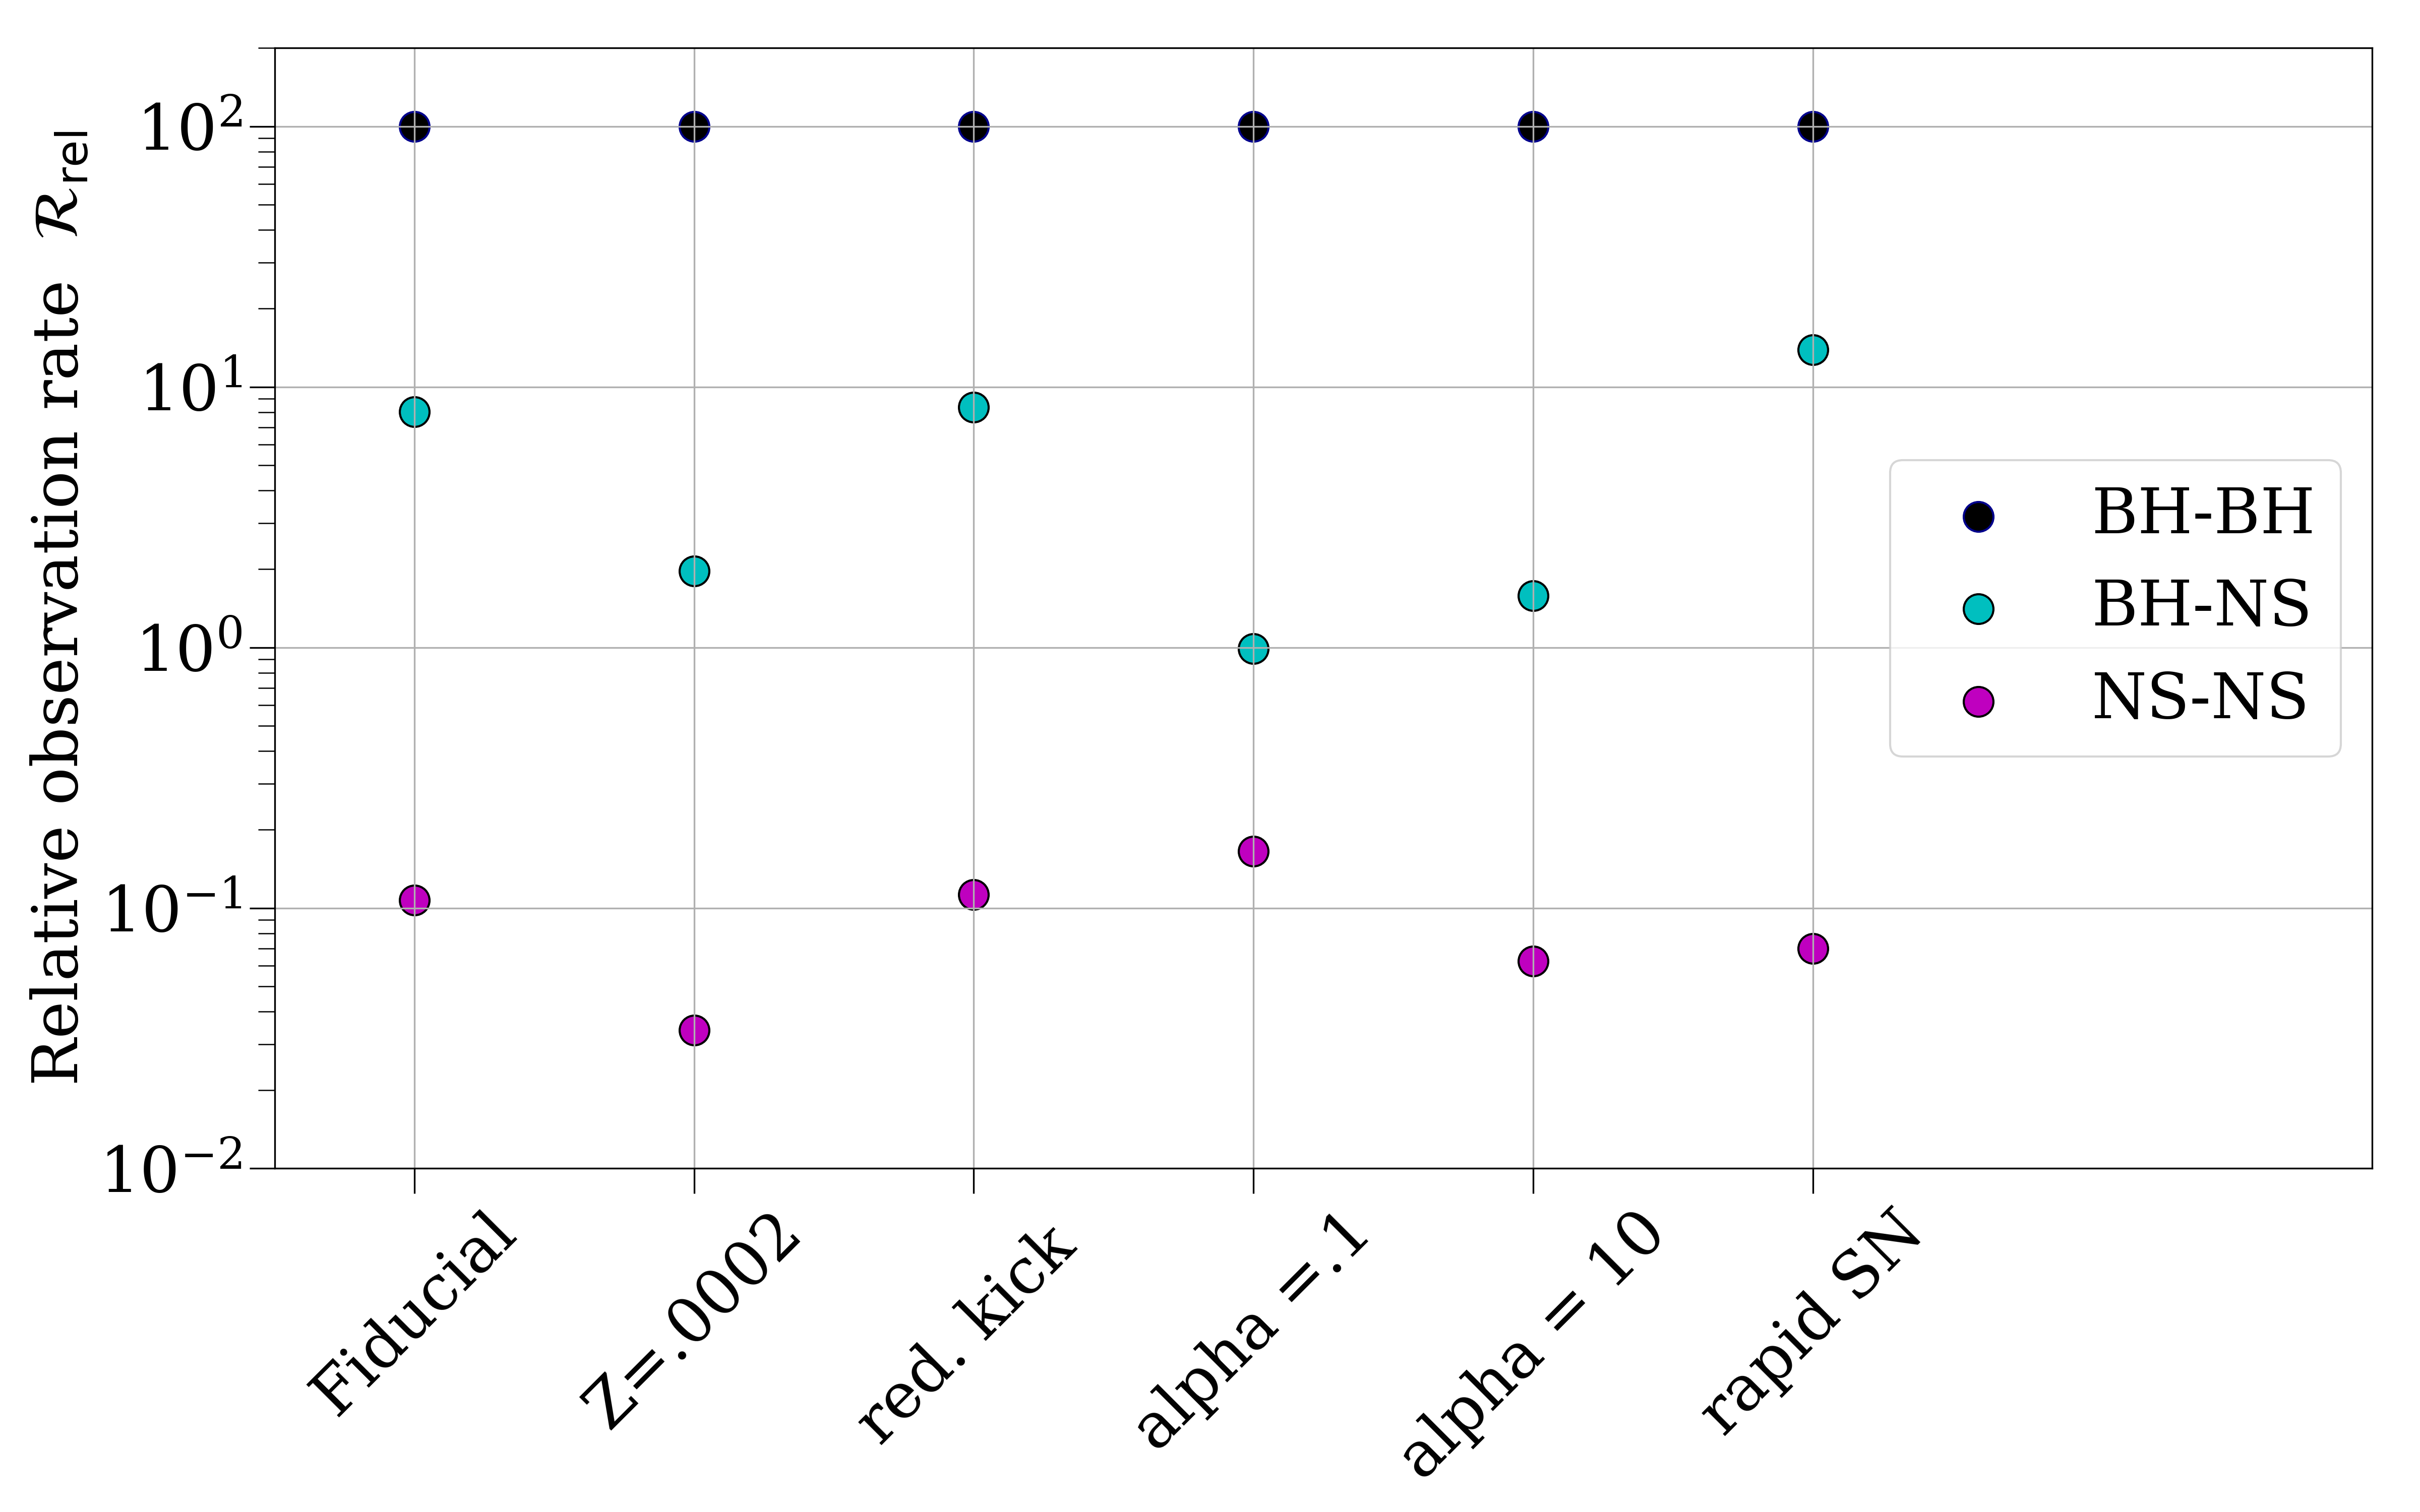
\includegraphics[width=.8\textwidth]{../PlottingScripts/imagesUFDandRatios/relativerates_observed.png}
%   \caption{ }
%  \label{fig:BHNS_DCO_k}
%\end{figure*}
%%

%\subsubsection{properties in vsys and time frame, and eccentricity versus separation frame }
%
%\begin{figure*}
%	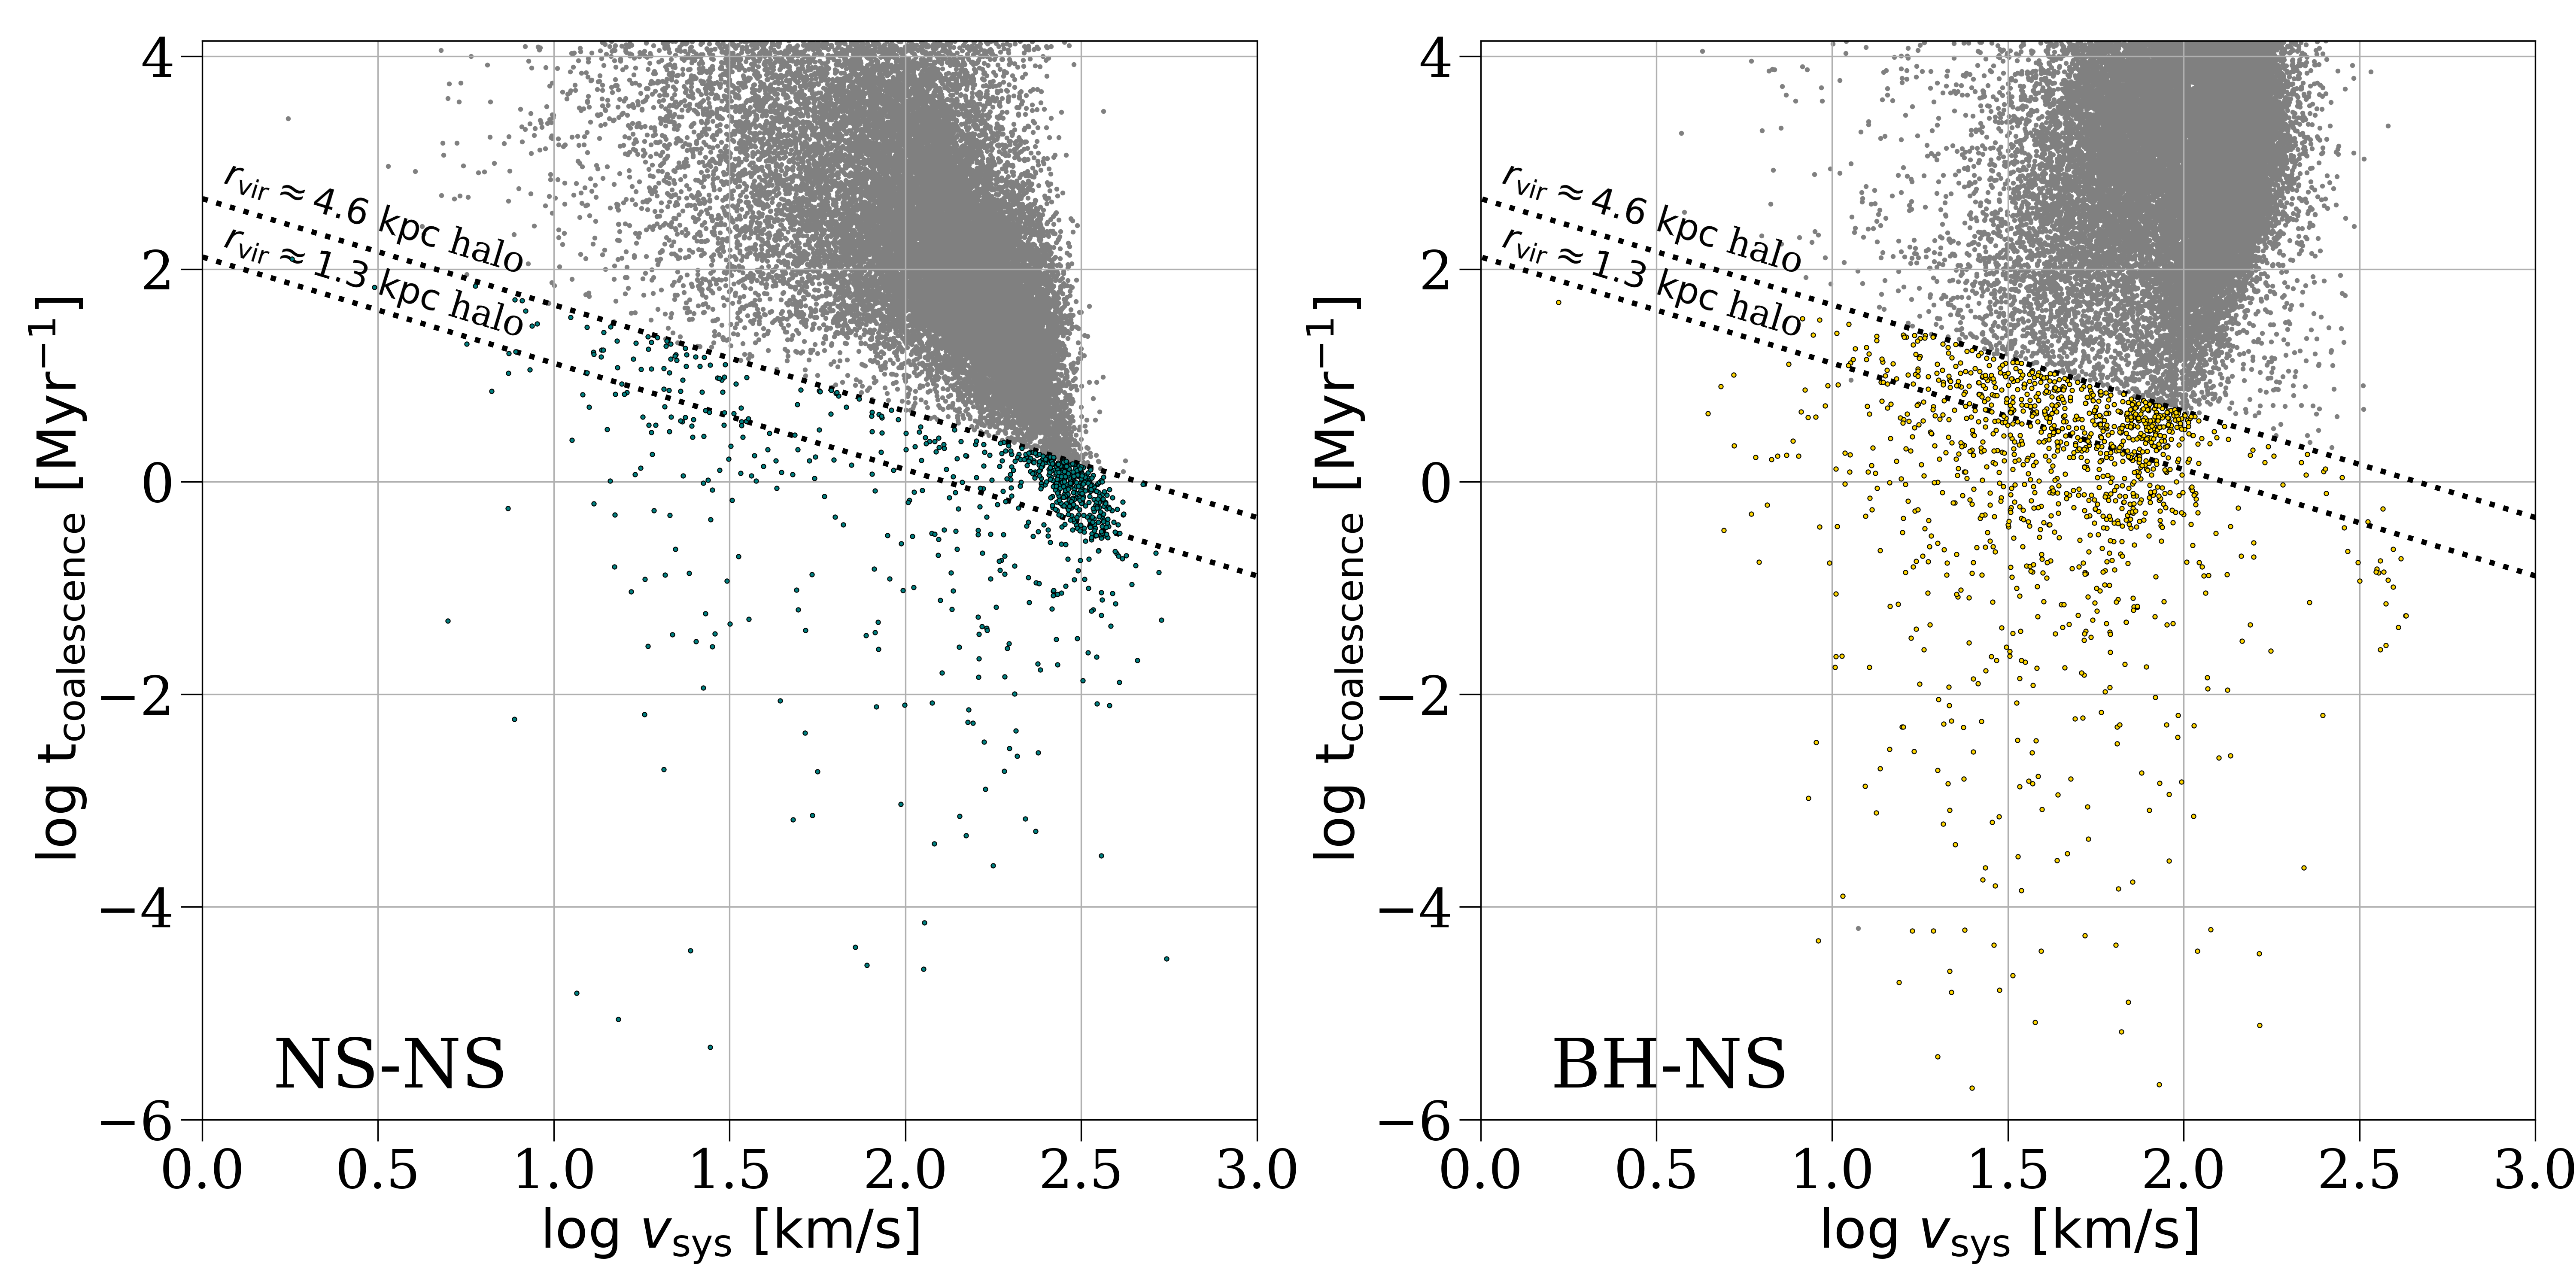
\includegraphics[width=1\textwidth]{../PlottingScripts/imagesUFDandRatios/scatterCandidates_Xeff.pdf} %CPUVsUncertaintySingleTogether.pdf}
%    \caption{The systematic velocity of the binary system versus the coalescence time, at the moment the double compact object formed. \textbf{[left panel:] } \ac{NSNS} mergers and candidates,   \textbf{[right panel:] } BH-NS mergers and candidate systems when assuming a high spinning \ac{BH} with  $\chi_{\rm{bh}} = 0.97$. In grey all double compact object mergers of that modeled population. A small subset of those mergers, merges well within the radius of a halo of $10^9 M_{\odot} \ (r_{\rm{vir}}   = 4.6 \, \rm{kpc})$ at $z \approx 6$ or a halo of mass   $10^8 M_{\odot} $ $ (r_{\rm{vir}}   = 1.3 \, \rm{kpc})$ at $z \approx 10$.   Dotted lines indicate the maximum $v_{\rm{sys}} \times t_{\rm{coalescence}}$ that is needed to merge within those halos}
%    \label{fig:NbinariesVsNHits}
%\end{figure*}


%
%\begin{figure*}
%	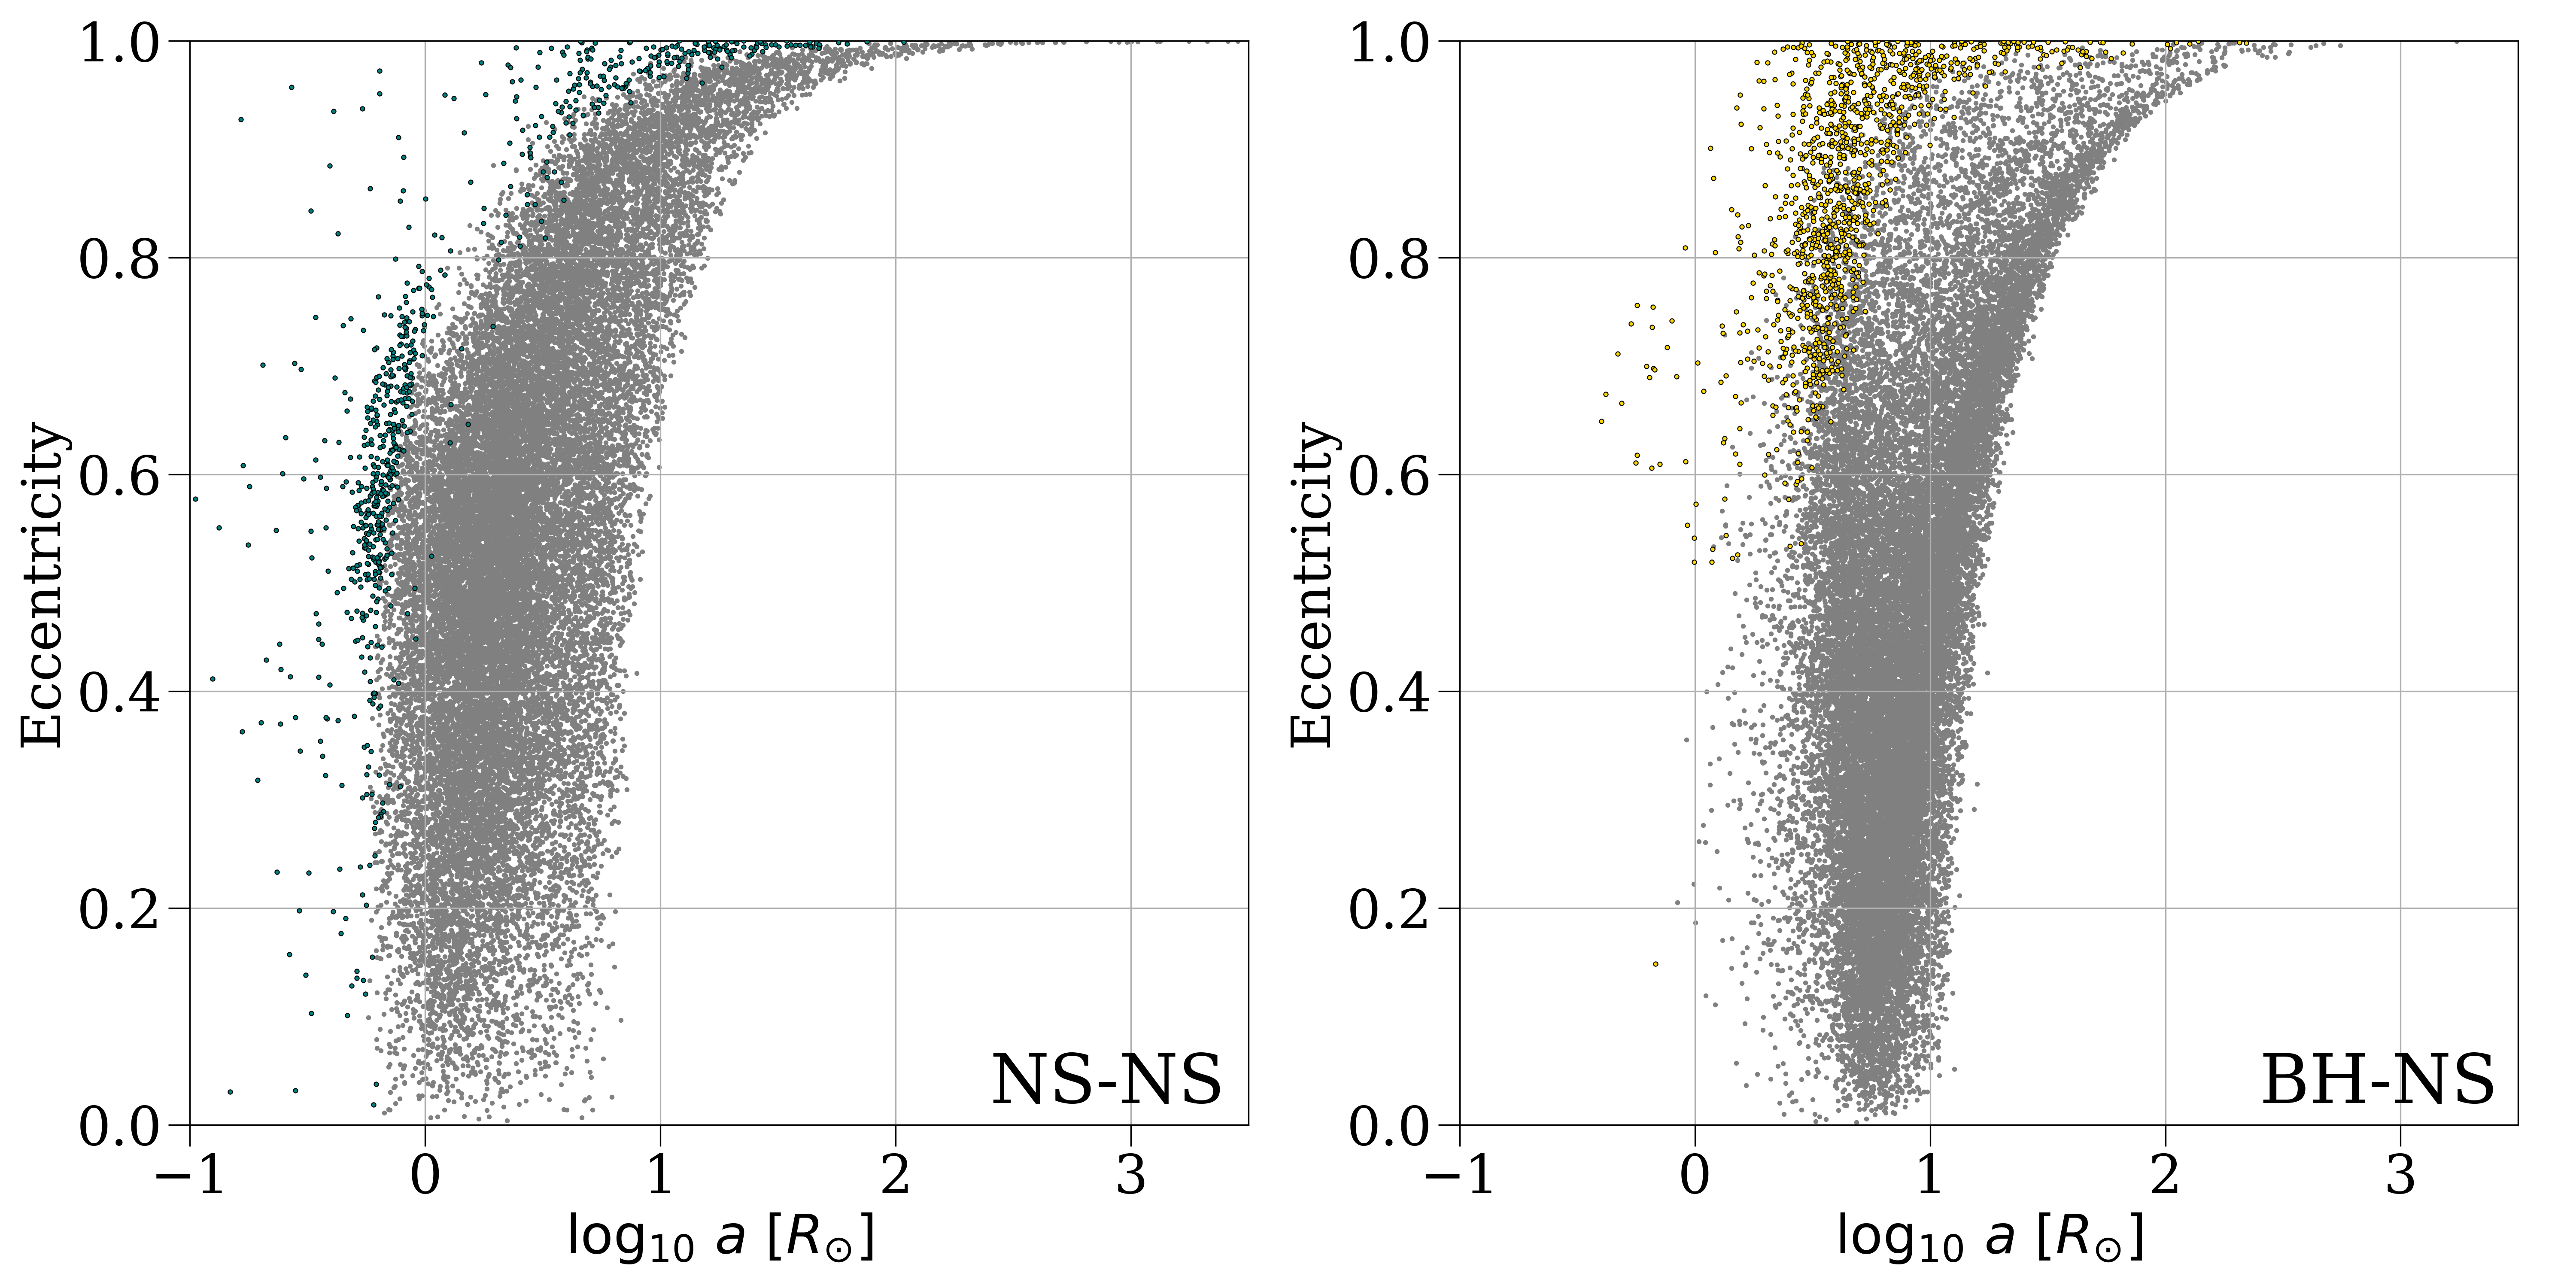
\includegraphics[width=1\textwidth]{../PlottingScripts/imagesUFDandRatios/scatterCandidates_Xeff_II.pdf} %CPUVsUncertaintySingleTogether.pdf}
%    \caption{The separation  of the binary system versus the eccentricity at the moment the double compact object formed. The systems that merge well within the halo of an UFD are coloured with blue or yellow.  \textbf{[left panel:] } \ac{NSNS} mergers and candidates,   \textbf{[right panel:] } BH-NS mergers and candidate systems when assuming a high spinning \ac{BH} with  $\chi_{\rm{bh}} = 0.97$. In grey all double compact object mergers of that modeled population.}
%    \label{fig:NbinariesVsNHits}
%\end{figure*}


%\subsubsection{properties of the candidate systems}
%\begin{itemize}
%	\item systematic velocities
%	\item natal kick properties
%	\item \ac{BH} vs \ac{NS} forms first  (do this here or in formation channel discussion) 
%	\item traveled distance
%\end{itemize}
%%
%\begin{figure*}
%	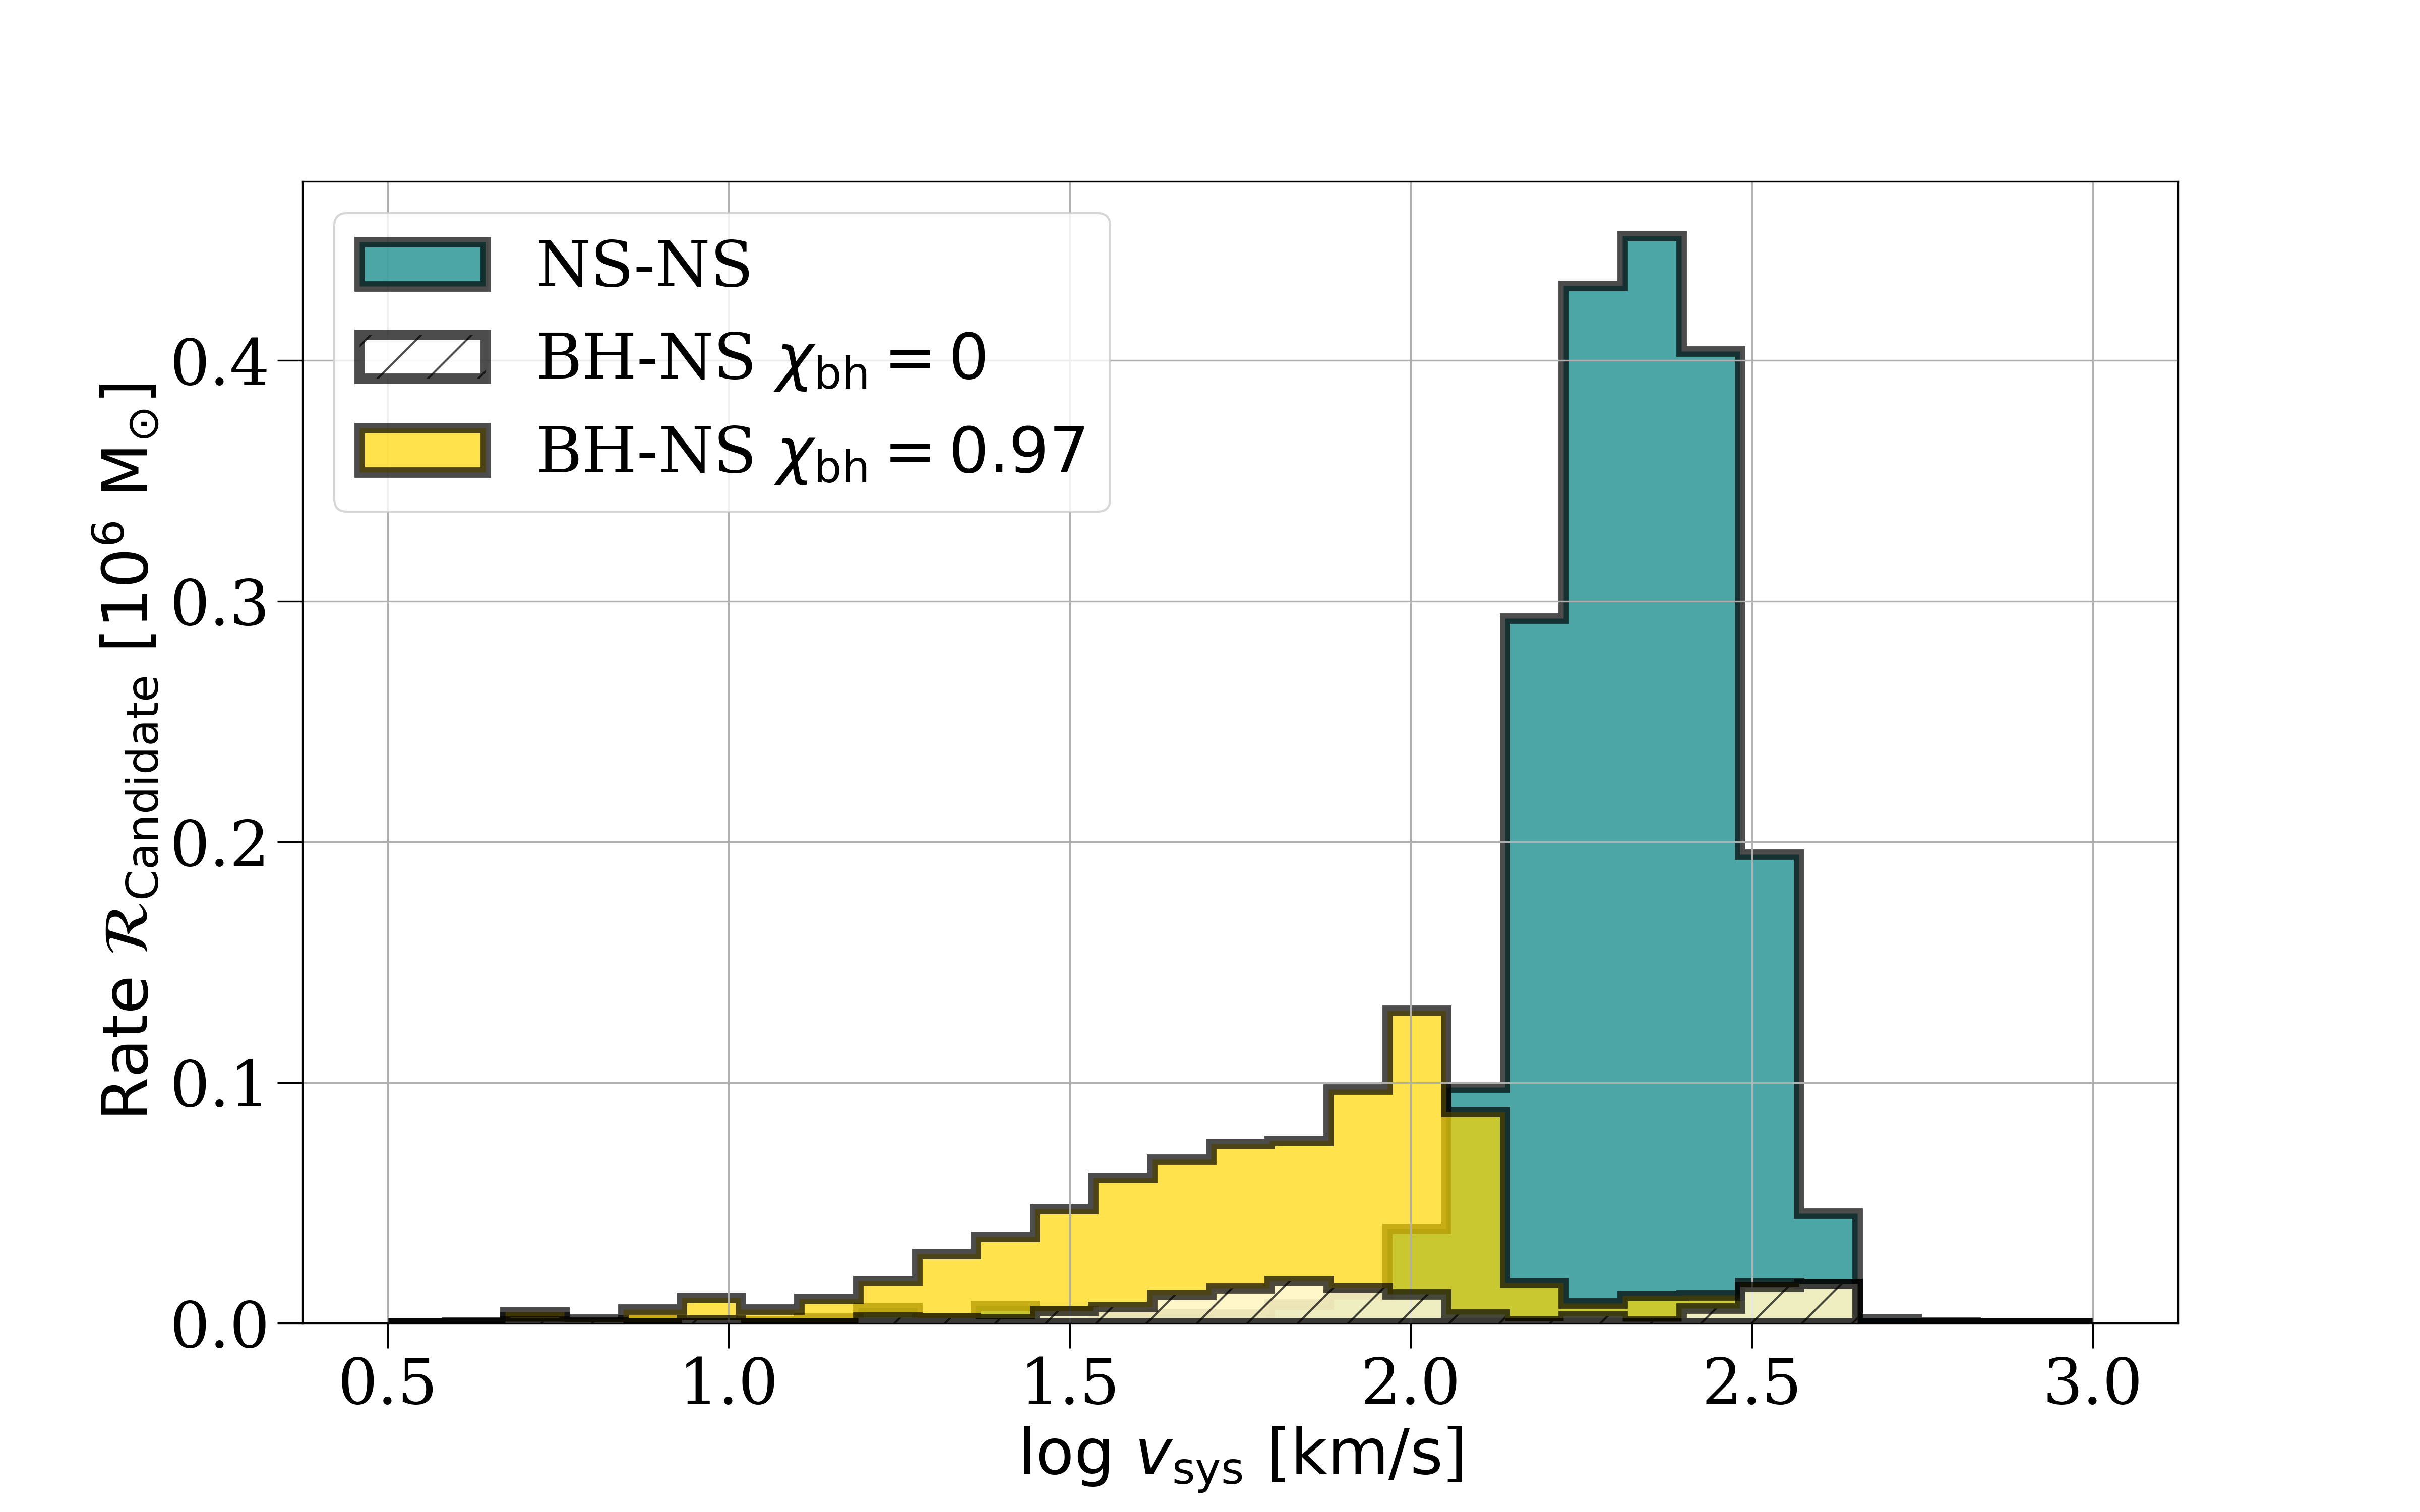
\includegraphics[width=1\columnwidth]{../PlottingScripts/imagesUFDandRatios/tsystematicPDF.pdf} %CPUVsUncertaintySingleTogether.pdf}
%    \caption{Distribution function of the systematic velocity of the candidate binaries after the second supernova. In blue the distribution for \ac{NSNS} candidates are shown, whereas in yellow the distribution for BH--NS systems is shown assuming a black hole spin of  $\chi_{\rm{bh}} = 0.97$ (where the hatched  area shows the distribution of BH--NS candidates if $\chi_{\rm{bh}} = 0$. It is clearly visible that \ac{NSNS} and BH--NS candidates have a distinct distribution function for $v_{\rm{sys }}$ with BH--NS having overall smaller systematic velocities}
%%    The number of binaries found of the target population  $N_{\mathrm{T}}$ as a function of the total number of binaries $N_{\text{binaries}}$ sampled for the traditional sampling method (gray dashed line) and the sampling method presented in this study (solid colored line). The four different panels show the simulations for each of the four target subpopulations. In each panel the duration of the exploratory phase is shown with a hashed gray area.  In the background the standard Poisson fractional uncertainties  of $0.3, 1$ and $3\%$ are shown with a dashed line.  } 
%    \label{fig:NbinariesVsNHits}
%\end{figure*}
%


%\begin{figure*}
%	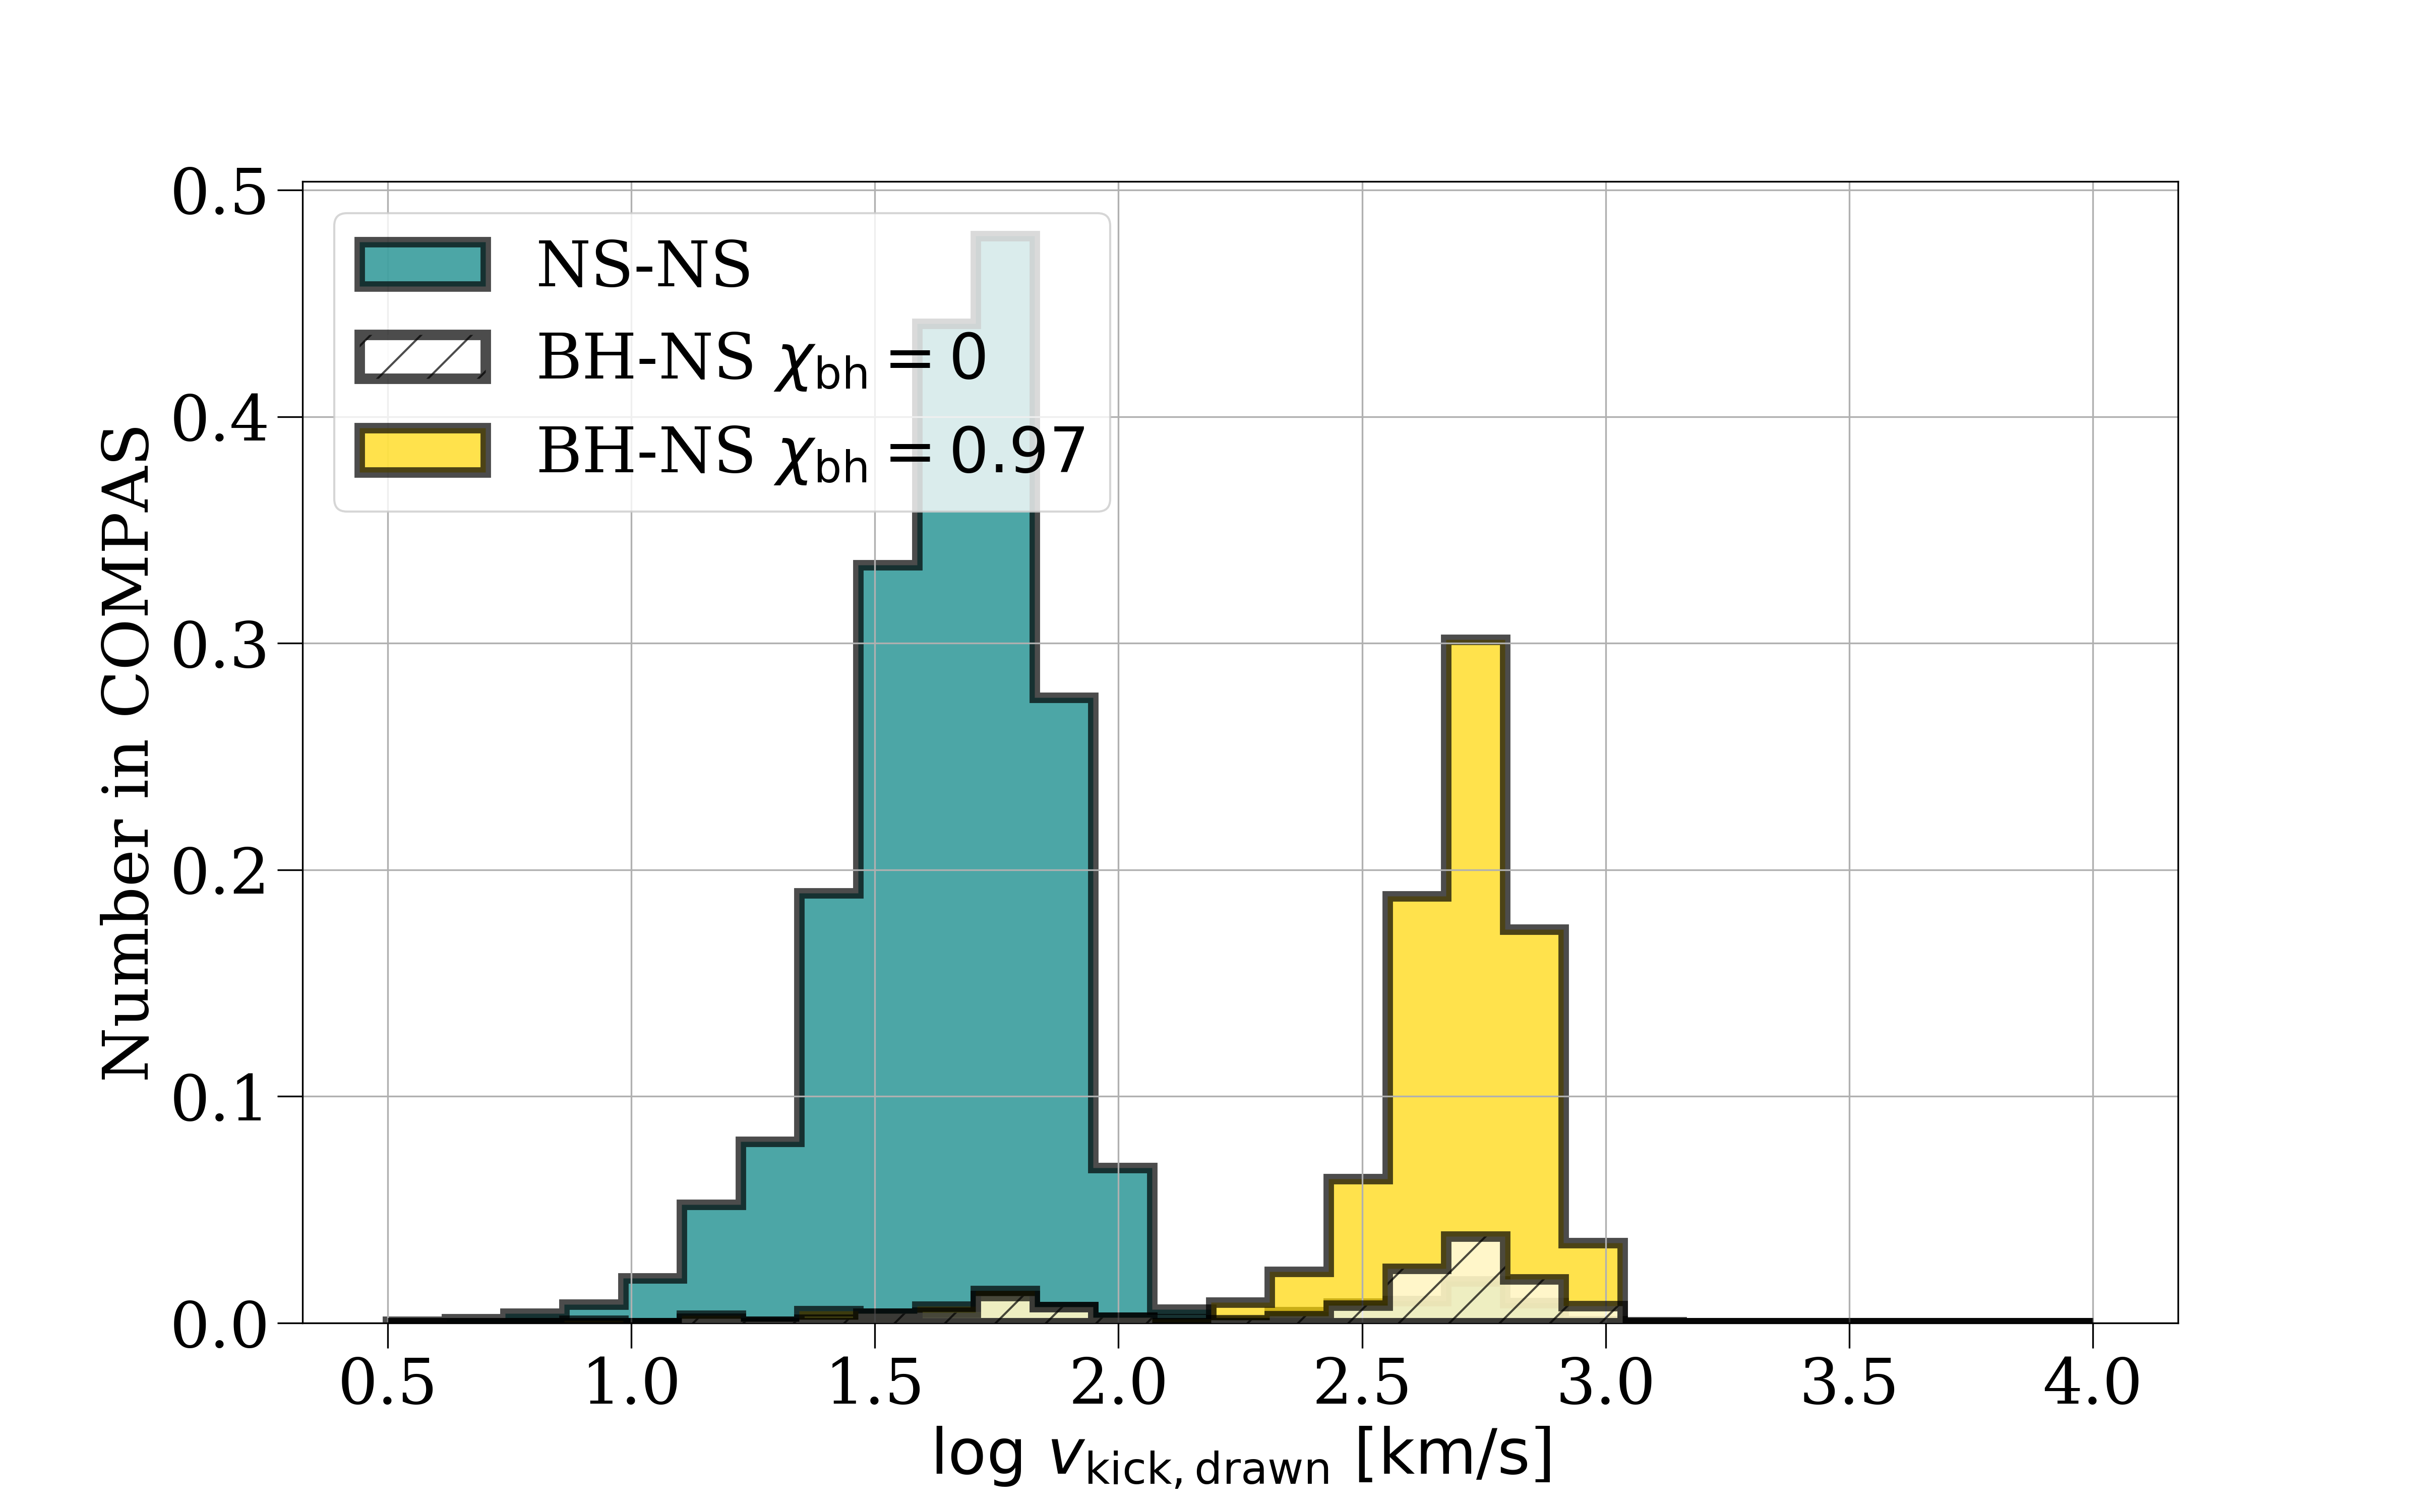
\includegraphics[width=1\columnwidth]{../PlottingScripts/imagesUFDandRatios/drawnKickVelocityPDF.pdf} %CPUVsUncertaintySingleTogether.pdf}
%    \caption{Distribution function of the drawn kick velocity magnitudes of the candidate binaries after the second supernova. In blue the distribution for \ac{NSNS} candidates are shown, whereas in yellow the distribution for BH--NS systems is shown assuming a black hole spin of  $\chi_{\rm{bh}} = 0.97$ (where the hatched  area shows the distribution of BH--NS candidates if $\chi_{\rm{bh}} = 0$. It is clearly visible that \ac{NSNS} and BH--NS candidates have a distinct distribution function for $v_{\rm{k }}$ with BH--NS having overall larger drawn kick velocities.}
%%    The number of binaries found of the target population  $N_{\mathrm{T}}$ as a function of the total number of binaries $N_{\text{binaries}}$ sampled for the traditional sampling method (gray dashed line) and the sampling method presented in this study (solid colored line). The four different panels show the simulations for each of the four target subpopulations. In each panel the duration of the exploratory phase is shown with a hashed gray area.  In the background the standard Poisson fractional uncertainties  of $0.3, 1$ and $3\%$ are shown with a dashed line.  } 
%    \label{fig:NbinariesVsNHits}
%\end{figure*}
%

%%
%\begin{figure*}
%		\includegraphics*[width=1\columnwidth]{../PlottingScripts/imagesUFDandRatios/traveldistancePDF_Xeff0_97.pdf}
%		\includegraphics*[width=1\columnwidth]{../PlottingScripts/imagesUFDandRatios/traveldistanceCDF_Xeff0_97.pdf}
%%
%%    \label{fig:RateCandidateEnriching}
%%\end{figure*}
%%%
%%%
%%\begin{figure*}
%		\includegraphics*[width=1\columnwidth]{../PlottingScripts/imagesUFDandRatios/traveldistancePDF_Xeff0_0.pdf}
%		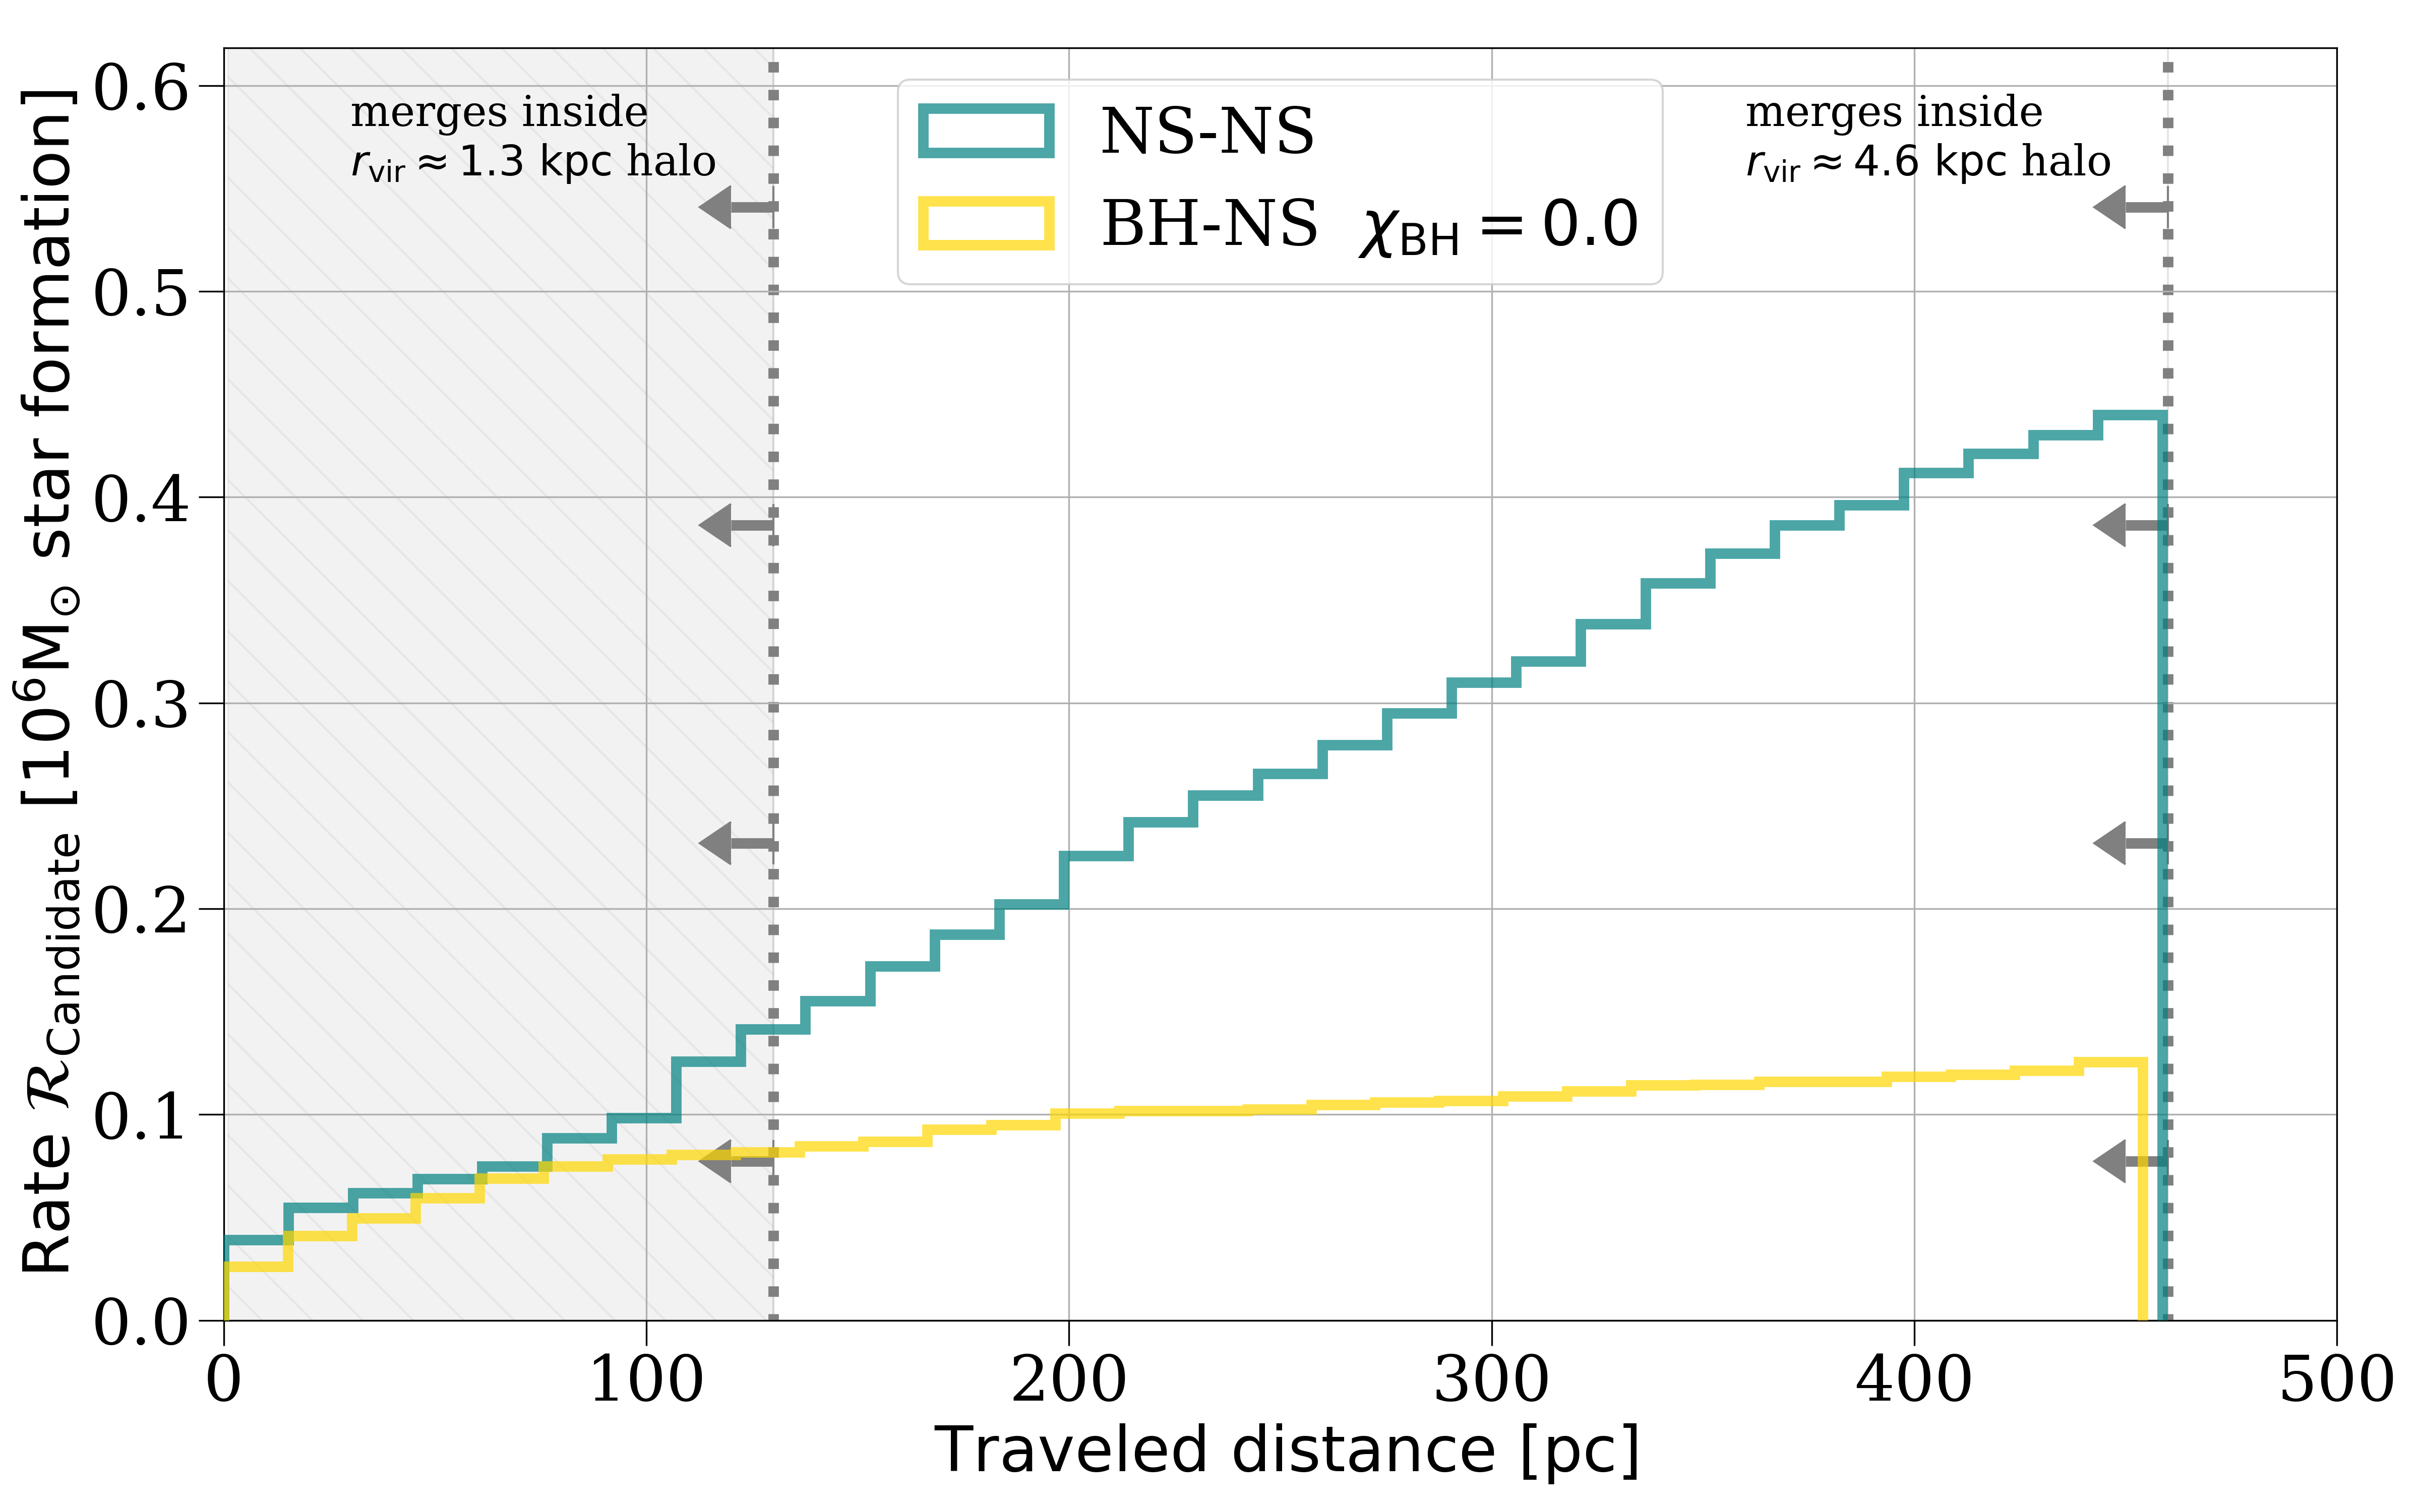
\includegraphics[width=1\columnwidth]{../PlottingScripts/imagesUFDandRatios/traveldistanceCDF_Xeff0_0.pdf}
%    \caption{\textbf{Left panel:} distribution function and \textbf{right panel:} cumulative distribution function of the travelled distance of the candidate binaries between the second \ac{SN}  and the merger. In blue the distribution for \ac{NSNS} candidates are shown, whereas in yellow the distribution for BH--NS systems is shown. \textbf{Upper panel:}  assuming a black hole spin of  $\chi_{\rm{bh}} = 0.97$. \textbf{lower panel:} the same but now assuming BH--NS candidates have a black hole with spin $\chi_{\rm{bh}} = 0$.  BH--NS candidate rates are similar for both assumed halos if the black holes have a high spin, whereas if black holes have negligible spin, the BH--NS become mostly important for lower mass halos. } 
%    \label{fig:RateCandidateEnriching}
%\end{figure*}

%%
%\subsubsection{rates comparison with UFD galaxies}
%%
%\begin{figure*}
%		\includegraphics[width=1\textwidth]{../PlottingScripts/imagesUFDandRatios/RateUFDEnrichingMergers2.pdf}
%		\includegraphics[width=1\textwidth]{../PlottingScripts/imagesUFDandRatios/RateUFDEnrichingMergers2_Rvir1_3.pdf}
%    \caption{ The formation rate of candidate  \ac{NSNS} (first cirlce data point) and BH--NS (square data points) binaries. Each data point indicates the total rate of formation of candidate systems per $10^6 \ \rm{M}_{\odot}$ star formation. There are one circle and 6 squares which correspond to the one \ac{NSNS} model and 6 BH--NS models studied here. In grey for each model the rate of all double compact mergers in a Hubble time is given. A fraction of those mergers, mergers well within the ultra-faint-dwarf galaxy, possibly makes r-processes  and merges fast enough to be able to explain the r-process enriched UFD. The rate of those candidate systems are shown with a coloured datapoint. For BH--NS candidate mergers the rate of candidate systems depends on the assumption for the black hole spin which is is shown with the colorbar} 
%    \label{fig:RateCandidateEnriching}
%\end{figure*}

%
%
%
%%
%\subsubsection{Evolutionary channels of the fast merging systems}
%\label{sec:evolutionchannels}
%



\section{Conclusions}
\label{sec:conclusions}
%
In this study we make predictions for  observations 
of \bhnsSingle mergers by a ground-based  \ac{GW} detectors at design sensitivity. We accomplish this by simulating populations of binaries over a grid of 50 metallicities and taking into account the cosmic star formation history and detection probability. We explore both uncertainties arising  from massive binary star evolution and not knowing the star formation history (\ac{MSSFR}) and in this way obtain \Nmodels (\NmodelsBPS binary population synthesis $\times$ \NmodelsMSSFR \ac{MSSFR} variations) different models that lie within our model uncertainties. 

Our main findings  are summarized below:



\subsection{Predictions for \bhnsSingle mergers from our Fiducial model}

\begin{itemize}
\item Our fiducial model (\mAzero) predicts an intrinsic  \bhnsSingle merger rate at redshift zero of $\RateIntrinsicZero = \RateIntrinsicAzeroBHNS $\GpcminThree \yearmin  consistent with the upper limit inferred from the first and second observing run of the LVK network   \citep{2019PhRvX...9c1040A}. When weighting for the sensitivity  of a ground based \ac{GW} network we find a detection rate of $\RateObserved = \RateObservedAzeroBHNS $\yearmin. 
Assuming 50 \ac{BHBH} mergers will be detected in the third observing run from the LVK network our \bhnsSingle rate rescales to $\RateObserved^{\rm{O3}} \approx 1 $ \bhnsSingle detections expected in O3. 


\item  Our fiducial model predicts that 90$\%$ of  the \ac{GW} observed \bhnsSingle mergers formed through the \textit{classic CE} channel within isolated binary evolution. This channel involves  first a stable mass transfer episode, and eventually a reversed  unstable \ac{CE} mass transfer phase. 
This is different compared to \ac{BHBH} and \ac{NSNS} mergers where we predict $70\%$ and $60\%$ of the \ac{GW} detected mergers forms through the \textit{only stable mass transfer} and \textit{double-core \ac{CE}} channel respectively. 
\ac{GW} observations of \bhnsSingle mergers  therefore provide a good probe to study the classic \ac{CE} channel without having contamination from other channels within the isolated binary evolution scenario. 

\item Our fiducial model predicts that a fraction between 2--24$\%$ of \ac{GW} detected \bhnsSingle mergers will disrupt the \ac{NS} outside of the \ac{BH} inner-most-stable-orbit. Such systems are thought to produce electromagnetic transients that could possibly be observed as counterparts to their \ac{GW} observations. 
\end{itemize}





\subsection{Varying binary population synthesis and \ac{MSSFR} models}

\begin{itemize}
\item We find that the \bhnsSingle rate predictions can change two orders of magnitude from binary population synthesis uncertainties and an order of magnitude from \ac{MSSFR} uncertainties. From the combination of models we obtain predicted rates in the ranges $\RateIntrinsicZero \in [ \RateIntrinsicAzeroBHNSmin,  \RateIntrinsicAzeroBHNSmax]\GpcminThree \yearmin$ and $\RateObserved \in [ \RateObservedAzeroBHNSmin,  \RateObservedAzeroBHNSmax]$\yearmin, which gives an overall  spread  between  the minimum and maximum predicted \bhnsSingle rate  of  $\approx 250\times$.


\item we find for our \Nmodels model variations that the predicted fraction of \ac{GW} detectable \bhnsSingle mergers where the \ac{NS} is disrupted outside of the \ac{BH} lies in the range $f_{\rm{EM}} \sim [0, 0.57]$. The lowest fraction is for the rapid supernova and 11.5\km NS radii and 0 \ac{BH} spin, whereas the highest fraction is also for the rapid SN model but assuming 13\km NS radii and 0.5 BH spins. 

\item We find that the fraction of \bhnsSingle mergers where the NS forms first  (NS--BHs) is sensitive to binary population and \ac{MSSFR} variations and can vary in the range $[0.0011, 0.28]$. The optimistic CE model (B) and high mass transfer efficiency model (J) give distinguishable high NS--BH fractions. This fraction could be possibly inferred from the spins of \ac{GW} observations and the rate of pulsar--BH systems. 


\item We find that the shape of the \bhnsSingle distributions is dominated  by the variations in  binary population synthesis assumptions rather than \ac{MSSFR}. 



\item We find that the $90\%$ confidence intervals of the observed \bhnsSingle mergers are predicted to have  \ac{BH} masses in $[2.5, 15]$\Msun and that in none of our model variations more than 1$\%$ of the detections will have BH mass above 25\Msun. This is different compared to dynamical formation where such systems are much more common. 


\item We find that \bhnsSingle mergers with \acp{BH} with $\mbhf \leq 5\Msun$  are predicted to be commonly detected. \bhnsSingle mergers with \acp{NS} with $\mnsf \geq 1.8\Msun$ are also common in all our models except model F (rapid SN remnant mass function). 

\item We find that \bhnsSingle mergers have unequal mass ratios with the median mass ratio typically being $\qf \geq 5$ for our model variations.  

%\item We find that in all our models at least $90\%$ of the \bhnsSingle mergers are predicted to have mass ratios in the range $[1. 8]$

\end{itemize}



\subsection{Comparison with \ac{BHBH} and \ac{NSNS} mergers}



\begin{itemize}

\item Considering \Nmodels model variations we find predicted intrinsic \ac{BHBH} and \ac{NSNS} rates in the ranges 
$\rate_{\rm{m}}^{0,\rm{BHBH}} \sim [ \RateIntrinsicAzeroBHBHmin,  \RateIntrinsicAzeroBHBHmax]$\GpcminThree \yearmin and \ac{GW} detectable rates of   $\rate_{\rm{m}}^{0,\rm{NSNS}} \sim [ \RateIntrinsicAzeroNSNSmin,  \RateIntrinsicAzeroNSNSmax]$\GpcminThree \yearmin. 
Our fiducial model predicts merger rates of  $\rate_{\rm{m}}^{0,\rm{BHBH}} \approx  \RateIntrinsicAzeroBHBH$\GpcminThree \yearmin and  $\rate_{\rm{m}}^{0,\rm{NSNS}} \approx  \RateIntrinsicAzeroNSNS$\GpcminThree \yearmin for \ac{BHBH} and \ac{NSNS} mergers respectively.  


\item We find that most \ac{MSSFR} models overpredict the observed \ac{BHBH} rate (Figure~\ref{fig:IntrinsicRatesBBHBNSBHNS}).  Indicating that the \ac{MSSFR} prescriptions leading to lower rates are preferred.  We also find that all binary population and \ac{MSSFR} variations underpredict the observed NSNS rate except model L that has low NS kicks. This suggest that  binary population synthesis models with higher NSNS merger rates such as model L with low  NS kicks are preferred. Alternatively,  the current \ac{GW} observed rate might be an overprediction due to the low number of NSNS detections, or a different formation channel than the isolated binary evolution channel is contributing to the observed NSNS rate. 



\item We find that among the \ac{DCO} types the \ac{BHBH} merger rates are mostly sensitive to variations in \ac{MSSFR} which impacts the BHBH rate with factors  $\langle \sigma_{\rm{xyz}}\rangle  \approx 18$ and $\approx 44$, whereas 
the binary population variations impact the rate with a factor $\langle \sigma_{\rm{\mu}}\rangle \approx 6$. For \bhnsSingle and \ac{NSNS} mergers, on the other hand, the binary population synthesis variations dominate the rate with $\langle \sigma_{\rm{\mu}}\rangle \approx 32$ and $\approx 30$ for \bhnsSingle and  $ \langle \sigma_{\rm{\mu}}\rangle \approx 320$ and $\approx 215$  for NSNS versus $\langle \sigma_{\rm{xyz}}\rangle  \approx 10$ for \bhnsSingle and $\langle \sigma_{\rm{xyz}}\rangle  \approx 5$ for NSNS.  We thus find that BHBH rates constrain \ac{MSSFR} but not binary population synthesis whereas the observed  \bhnsSingle and NSNS rates are mostly informative for binary population synthesis assumptions. 

\item Compared to BHBH and NSNS, the predicted shape of the \ac{GW} distributions for \bhnsSingle mergers are very sensitive to binary population synthesis variations. Both the total mass,  chirp mass and mass ratio distributions for \bhnsSingle mergers have distinguishable predictions between binary population synthesis simulations and are robust for variations in \ac{MSSFR}. This is different from BHBH mergers where the shape of the distributions are barely impacted by binary population synthesis variations and only impacted by some changes in \ac{MSSFR} (e.g. models 113, 213 and 313). For the NSNS mergers distributions only two of our models are very distinguishable (model E and F) whilst the  other model variations and variations in \ac{MSSFR} do not strongly impact the shape of the NSNS distributions. This means that the \bhnsSingle merger distributions are a better probe to explore a broad range of binary population synthesis assumptions compared to NSNS and BHBH. 


\item Compared to BHBH and NSNS, \bhnsSingle mergers have lower mass \acp{BH} and are predicted to commonly have \acp{BH} with masses $\mbhf \leq 6 \Msun$. Our models predict that \bhnsSingle mergers will have more massive \acp{NS} compared to NSNS mergers where the NS masses are typically below 1.4\Msun. \bhnsSingle mergers are therefore a good probe to study the lower \ac{BH} remnant mass gap and the formation of massive \acp{NS}. 

\end{itemize}




All in all, we find that the observed \bhnsSingle rates together with the inferred population characteristics can help rule out massive binary population synthesis models. Ruling out \ac{MSSFR} models is more difficult and will require constraining the binary population synthesis result first as the variation in both the rate and shape of the distributions are dominated by binary population synthesis simulations.  We have shown that the rate and shape of the \bhnsSingle distributions can in many cases be more informative to rule out binary population synthesis models.  Simultaneous constrains from BHBH, \ac{NSNS} and other constrains from pulsar-BH and binary pulsar observations will help in the future to learn from \ac{GW} observations about massive binary evolution and cosmic history. 



\section*{Acknowledgements}
%
FSB thanks Lieke van Son, Serena Vinciguerra, Mathieu Renzo,  Angus Beane, Griffin Hosseinzadeh,  Lokesh Khandawal, Thomas Wagg, Floris Kummer,  Carl Rodriguez, Reinhold Willcox and Joel Leja for helpful discussions and input on this manuscript. FSB thanks Victoria diTomasso, Miranda Eiben and Locke Patton for crucial input that was important  for finishing this project.  In addition, FSB  especially thanks David Stops and the Harvard FAS research computing group for technical support on the simulations and high performance computing part of the research.   Lastly, FSB wants to acknowledge the  amount of luck and privilege that was involved to end up pursuing this astronomy research. 
SJ thanks Chris Fryer. FSB is supported in part by the Prins Bernard Cultuurfonds studiebeurs 2020. 

Facilities: \\ 
FAS Research Computing, Birmingham computer cluster. 

Software: \\
\textsc{COMPAS}  \citep{stevenson2017formation, 2018MNRAS.477.4685B, 2018MNRAS.481.4009V},   \texttt{Python} available from \url{python.org}, matplotlib \citep{2007CSE.....9...90H},  \texttt{NumPy} \citep{2011CSE....13b..22V}, \texttt{ipython$/$jupyter} \citep{2007CSE.....9c..21P, kluyver2016jupyter} This paper used the \texttt{Astropy} library \citep{2018AJ....156..123A}.

 {\sc{SEOBNRv3}} and  {\sc{IMRPhenomPv2}}

%
%The Berger Time-Domain Group is supported in part by NSF grant AST-1714498 and NASA grant NNX15AE50G. G.H. thanks the LSSTC Data Science Fellowship Program, which is funded by LSSTC, NSF Cybertraining Grant \#1829740, the Brinson Foundation, and the Moore Foundation; his participation in the program has benefited this work. F.D.\ thanks the SAO REU program, funded in part by the National Science Foundation REU and Department of Defense ASSURE programs under NSF Grant no.\ AST-1852268 and by the Smithsonian Institution. V.A.V.\ acknowledges support by the National Science Foundation through a Graduate Research Fellowship.


This research has made use of data, software and/or web tools obtained from the \ac{GW} Open Science Center (\url{https://www.gw-openscience.org}), a service of LIGO Laboratory, the LIGO Scientific Collaboration and the Virgo Collaboration. LIGO is funded by the U.S. National Science Foundation. Virgo is funded by the French Centre National de Recherche Scientifique (CNRS), the Italian Istituto Nazionale della Fisica Nucleare (INFN) and the Dutch Nikhef, with contributions by Polish and Hungarian institutes.
%
%%%%%%%%%%%%%%%%%%%%%%%%%%%%%%%%%%%%%%%%%%%%%%%%%%
%
%%%%%%%%%%%%%%%%%%%% 




\bibliography{my_bib}{}
\bibliographystyle{aasjournal}







%% This command is needed to show the entire author+affiliation list when
%% the collaboration and author truncation commands are used.  It has to
%% go at the end of the manuscript.
%\allauthors

%% Include this line if you are using the \added, \replaced, \deleted
%% commands to see a summary list of all changes at the end of the article.
%\listofchanges




\newpage 
%%%%%%%%%%%%%%%%%%%%%%%%%%%%%%%%%%%%%%%%%%%%%%%%%%

%%%%%%%%%%%%%%%%% APPENDICES %%%%%%%%%%%%%%%%%%%%%

\appendix

%\onecolumn


\section{ \ac{SN} remnant function bug fix}
\label{sec:app-Fryer-bug-fix}
%


We fixed a bug in the implementation of the delayed Fryer remnant mass prescription  \citep{2012ApJ...749...91F} in  {\sc{COMPAS}}, which lead in previous simulations with the {\sc{COMPAS}} code to an additional gap in the neutron star remnant mass distribution around  2.2\Msun. This extra \ac{NS} mass gap around 2.2\Msun can be seen in e.g.   the middle panel of Figure~7 in \citealt{2018MNRAS.481.4009V} and bottom panels of Figure~7 in  \citealt{2019MNRAS.490.5228B}.  The current, and correct, implementation of the delayed Fryer remnant mass prescription leads to only one gap  in the neutron star remnant mass distribution around 1.7\Msun (see also Figure~\ref{fig:BHNS_DCOmasses}), which is in agreement with  \citet{2012ApJ...749...91F} (see e.g. their  Figure~12).  
The cause of the bug in {\sc{COMPAS}} was located in the calling of the baryonic mass function in the delayed remnant mass prescription of  \citet{2012ApJ...749...91F}. In the delayed remnant mass prescription, the final remnant (baryonic mass) is calculated from two equations  (Equation~12 and 13 in \citealt{2012ApJ...749...91F}), namely for stars that end up as NSs the baryonic mass is calculated by solving
%
\begin{align}
%
	\frac{M_{\rm{rem,bar}} - M_{\rm{rem}}}{\Msun} 
	= 0.075  \  
	\left(
	\frac{M_{\rm{rem}}}{\Msun}
	\right)^2
%
\label{eq:remnantNS}
\end{align}
%
whereas for stars that will end up as a \ac{BH} the equation
%
\begin{align}
M_{\rm{rem}} = 0.9 M_{\rm{rem,bar}}
\label{eq:remnantBH}
\end{align}
is used. Where $ M_{\rm{rem,bar}}$ is the baryonic remnant mass of the  star and $M_{\rm{rem}} $ is the final gravitational remnant mass (i.e. the final \ac{NS} or \ac{BH} mass). 

There is a small discontinuity in the remnant mass  for stars with masses exactly on the edge between these two equations, i.e.  between a \ac{NS} and a \ac{BH} as the former remnant masses are calculated using Equation~\ref{eq:remnantNS}, whereas the latter are calculated using Equation~\ref{eq:remnantBH}.  
Previously, {\sc{COMPAS}} placed this bifurcation at $M_{\rm{rem,bar}} = 2.5$\Msun, where $2.5$\Msun is our maximum assumed mass of a NS. However, the correct location of the bifurcation should be  at $M_{\rm{rem}} = 2.5$, which corresponds with $M_{\rm{rem,bar}} = 2.9669$. Where the number $M_{\rm{rem,bar}} = 2.9669$\Msun is found by solving $M_{\rm{rem,bar}}$ for $M_{\rm{rem}} = 2.5$ in Equation~\ref{eq:remnantNS}.

The bug and the correct remnant mass prescription is shown in Figure~\ref{fig:app-fryer2012-bug-fix}, which shows the mapping between the carbon-oxygen (CO) core masses to the final remnant mass $M_{\rm{rem}} $.  The  correct implementation of  the \citep{2012ApJ...749...91F} has a break in the remnant mass at $M_{\rm{rem}} =2.5$\Msun, which corresponds with switching from Equation~\ref{eq:remnantNS} to \ref{eq:remnantBH} at baryonic mass $M_{\rm{rem,bar}} =2.9669$ whereas in the old (bug) implementation {\sc{COMPAS}} switched between the equations at $M_{\rm{rem,bar}} =2.5$. The result is that previously, COMPAS was wrongly assigning slightly too high \ac{NS} masses (yellow hashed area) and was classifying some NSs that should have ended as \ac{BH}s (green area). 

%
\begin{figure}
\includegraphics[width=.5\columnwidth]{../fryer2012remnantBUG/remnantMassMnsmaxVariatios.png}
   \caption{Final remnant mass as a function of carbon-oxygen core mass based on the delayed remnant mass prescription of   \citet{2012ApJ...749...91F}. The red line shows the correct mapping, whereas the blue line shows the mapping caused by a small bug in {\sc{COMPAS}} that misplaced the break that decides whether to use the \ac{NS} or \ac{BH} equation to calculate the final gravitational remnant mass from the baryonic remnant mass.    }
%
  \label{fig:app-fryer2012-bug-fix}
\end{figure}
%




%\section{Renormalization of the formation rate from binary population synthesis simulation}
%\label{sec:app-calculating-rate-BPS}
%
%re normalization of BPS 
%
%Monte Carlo experiment explanation 
%
%In the end of the simulation we use the weights, and integrate over the missing parameter space (see Appendix X) to obtain a formation rate of \bhnsSingle mergers per star forming mass, delay time and chirp mass given by
%%
%\begin{align}
%%
%&\rate_{\rm{form}}(Z, \tdelay, \monef, \mtwof) =  
%\frac{\diff^4 \Nform}{\diff \MSFR \diff \tdelay \diff \monef \diff \mtwof} (Z, \tdelay, \monef, \mtwof). 
%%
%\end{align}
%%
%We assume stars to have masses in the range $0.08 $--$150$\Msun \citep{2004MNRAS.348..187W, 2005Natur.434..192F}, but see e.g. \citep{2018Sci...359...69S} that show evidence for a limit of 300\Msun, although this wouldn t really matter 
%








\section{Calculating the cosmological merger rates}
\label{sec:app-calculating-merger-distributionsMSSFR}
%
%

%To calculate the \bhnsSingle merger rate that is detectable with ground-based \ac{GW} interferometers today we follow a similar derivation as in e.g.  \citet{2013ApJ...779...72D, 2015ApJ...806..263D,2016ApJ...819..108B,2016MNRAS.458.2634M, 2019MNRAS.482..870E, 2019PhRvD.100f4060B,2019arXiv190612257B, 2019MNRAS.482.5012C}. The rate of \bhnsSingle mergers as a function of merger time \tmerger which can be calculated by a convolution $``{*}``$ of the metallicity-specific star formation rate (MSSFR) with the formation rate of \bhnsSingle mergers:
%
%%
%\begin{align}
%%
%	\rate_{\rm{m}} (\tmerger) &= 
%		\frac{\diff^4 \Nmerger }{\diff \ts \diff \Vc  \diff \monef \diff \mtwof}
%		 (\tmerger) 
%%
%		= \int \diff Z 
%				\left(  
%				{\rm{MSSFR}} \ 
%				{*}  \ 
%		 		\frac{\diff^4 \Nform}{\diff \MSFR \diff \tdelay  \diff \monef \diff \mtwof}  
%		  \right)
%		  (\tmerger) \notag \\
%%
%		&= \int \diff Z 
%		 \int_0^{\tmerger} 
%		 \diff \tdelay \, 
%		{\rm{MSSFR}}(\tform) \, \times 
%%		\, \hspace{4cm} 
%		\rate_{\rm{form}}(Z, \tdelay, \monef, \mtwof)  
%%
%\label{eq:app-merger-rate}
%\end{align}
%%
%
%where we used that $\tform = \tmerger - \tdelay$ where $\tform$ is the time in the Universe at which the binary was formed, and $\tdelay = \tevolve + \tinspiral$ is the time it takes the binary from formation to merge.  
%
%where \ac{MSSFR} is the metallicity-specific \ac{SFR} , which is obtained from  
%combining a \ac{SFR}   and  Metallicity density function 
%%
%\begin{align}
%{\rm{MSSFR}}(z) = \frac{d^3 \MSFR}{d \ts d \Vc dZ} (z)  = \underbrace{\frac{d^2 \MSFR}{d \ts d \Vc } (z)}_\text{SFR} \times \underbrace{\frac{d \MSFR }{dZ}(z)}_\text{GSMF $+$ MZR},
%\end{align}
%%
%
%where for our fiducial model we choose 
%
%\begin{align*}
%%
%{\rm{SFR}}(z)  =   \frac{\diff^2 \MSFR}{\diff \ts \diff \Vc} = a \frac{(1+z)^b}{1+ [(1+z)/c]^d}   \ \Msun \yearmin \MpcminThree 
%%
%\end{align*}
%%
%and 
%%
%\begin{align}
%\frac{\diff \MSFR }{\diff Z}(z) = \frac{1}{Z \sigma \sqrt{2 \pi}} \exp^{-\frac{(\log_{10}(Z) - \mu(z))^2}{2 \sigma^2}}.
%\end{align}
%%
%
%In the end we can calculate the observed merger rate by using 
%
%
%\begin{align*}
%%
%\rate_{\rm{det}}(\tdet, \monef, \mtwof) 
%= \frac{\diff^3 \Ndet}{\diff \tdet  \diff \monef \diff \mtwof}   
%= \int \diff \Vc  \, 
%\frac{\diff \ts}{\diff \tdet}  \, 
% \rate_{\rm{m}}(\tmerger) \,  
% \Pdet (\monef, \mtwof, \DL(z))
%%
%\end{align*}
%%
%using the substitution $\diff \Vc =  \frac{\diff \Vc}{\diff z} \diff z $ we obtain the integral over redshift
%%
%\begin{align}
%%
%\rate_{\rm{det}}(\tdet, \monef, \mtwof) = 
%	\int_0^{z_{\rm{max}}}  \diff z   \, 
%	\frac{\diff \ts}{\diff \tdet}(z)  \, 
%	\frac{\diff \Vc}{\diff z}(z) \,
%	 \rate_{\rm{m}}(z(\tmerger)) \,  
%	\Pdet (\monef, \mtwof, \DL(z)) 
%%
%\label{eq:Rdet-full-integral-form2}
%\end{align}
%%
%
%where we can fill in with the following (see e.g. \citealt{1999astro.ph..5116H}): 
%
%%
%\begin{align*}
%%
%\frac{\diff \ts}{\diff \tdet} = \frac{1}{(1+z)}
%%
%\end{align*}
%%
%is a factor to translate the source frame time $\ts$ to the detector frame. 
%%
%\begin{align*}
%%
%\frac{\diff \Vc}{\diff z}(z)  = \frac{4 \pi c}{\Hubble} \frac{\Dc^2(z)}{E(z)}
%%
%\end{align*}
%%
%with  $\Dc(z) = \frac{c}{\Hubble} \int_0^{z} \frac{ \diff z'}{E(z')} $   and  $E(z) = \sqrt{\Omega_{\rm{m}}(1+z)^3 + \Omega_{\Lambda}}$. \\
%
%
%
%
%$\Pdet$ is a function, with $\DL(z) = \Dc(z) (1+z)$.  \\
%
%filling this in together with Equation~\ref{eq:app-merger-rate} for the merger rate we obtain 
%\begin{align}
%%
%	&\rate_{\rm{det}}(\tdet, \monef, \mtwof)  = 
%	\int_0^{z_{\rm{m, max}}}  \diff z_{\rm{m}}  \,  \int  \diff Z \,  \int_0^{\tmerger}  \diff \tdelay \, \frac{1}{1 + z}   {\rm{MSSFR}}(z(\tform= \tmerger(z_{\rm{m}}-\tdelay)) \times \notag \\
%	&\hspace{4cm}
%	\rate_{\rm{form}}(Z, \tdelay, \monef, \mtwof)  
%	\frac{4 \pi c}{\Hubble} 
%	\frac{\Dc^2(z)}{E(z)} 
%	\Pdet (\monef, \mtwof, \DL(z)) 
%%
%\label{eq:Rdet-full-integral-form}
%\end{align}
%


Since we model only a fixed amount of metallicities $\Zi$ we approximate the integral in Equation~\ref{eq:rate_detector}  with the Monte Carlo estimate

%\begin{widetext}
\begin{equation}\label{eq:Upsilon}
    \boxed{
	\begin{aligned}
	%
	\rate_{\rm{det}}  =  
	\sum_{z_{{\rm{m}}}^j} \sum_{Z^k} \, 
 	%
	 \left( 
	 	\int_0^{\tmerger^j} \, %\tmerger(z_{{\rm{m}}}^j)
	 	 \diff \tdelay \, 
		 \rate_{{\rm{form}}}(Z^k, \tdelay, \monef, \mtwof)   \,
		 {\rm{MSSFR}}(z_{\rm{form}})   
	 \right) \times  
	%	
	 %
	   \frac{\Dc^2(z_{{\rm{m}}}^j) }{E(z_{{\rm{m}}}^j) }
	 \frac{1}{1 + z_{{\rm{m}}}^j}
 	 \frac{4 \pi c}{\Hubble} \
	  P_{{\rm{det}} }(\monef, \mtwof,z_{{\rm{m}}}^j) \,
	  %
	  \Delta z_{{\rm{m}}}^j \,
	  \Delta  Z^k, 
 %
	\end{aligned}
    }
\end{equation}
%\end{widetext}

where we sum over 100 equally divided  redshift bins $z_{{\rm{m}}}^j \in [0, z_{\rm{max}}]$ where we choose  $z_{\rm{max}} = 2$, which is a conservative upper limit for the maximum redshift ($z=2$ is equal to a luminosity distance of $D_{\rm{L}}\approx 1.5 \cdot 10^4$) out to which \bhnsSingle mergers are detectable with the LVK \ac{GW} network  (see Fig 3 of \citealt([][]{2016PhRvD..93k2004M} and see \citealt{2018LRR....21....3A}). 
We also sum over our 50 metallicity bins $Z^k \in [0.0001, 0.022]$, which are log-uniformly distributed.
 We use $\tmerger^j$ as short hand notation for $\tmerger(z_{{\rm{m}}}^j)$, the merger time at redshift $z_{{\rm{m}}}^j$, and also write 	the short hand notation  $ \Delta z_{{\rm{m}}}^j  = (z_{{\rm{m}}}^{j+1} - z_{{\rm{m}}}^j)$ and  $\Delta  Z^k = (Z^{k+1} - Z^{k})$. 
We also use $z_{\rm{form}}$ as a short hand notation for $z(\tform = \tdelay - \tmerger^j)$.  
\Dc and $E$ are functions of redshift given in \CMP  and  $\Hubble$ is the Hubble constant at redshift $z=0$.  


%\begin{table}[]
%\caption{Metallicity grid used in this study.}
%\label{tab:metallicity-values}
%\resizebox{\columnwidth}{!}{%
%\centering
%\begin{tabular}{|c|c|}
%\hline 
%\Zi & 0.0001, 0.00017783, 0.00031623, 0.00056234, 0.001, \\ 
% 	& 0.0011487, 0.00131951, 0.00151572 , 0.0017411, 0.002, \\
% 	& 0.0022974, 0.00263902, 0.00303143, 0.0034822, 0.004,\\
% 	& 0.00448144, 0.00502082, 0.00562513, 0.00630217, 0.0070607, \\
% 	& 0.00791052, 0.00886263, 0.00992933 ,0.01112443, 0.01246336 ,\\
% 	& 0.0142 ,0.01564408, 0.017527, 0.01963655, 0.022\\
%\hline 
%\end{tabular} 
%}
%\end{table}




%%
%\begin{table}
%\caption{Metallicity grid used in this study}
%\label{tab:metallicity-values}
%\resizebox{0.5\columnwidth}{!}{%
%\centering
%\begin{tabular}{lllr}
%\hline
%Model nr 	& Physics that is changed & Variation  			& nr$^{*}$    		\\ \hline
%\Zi & 0.0001, 0.00017783, 0.00031623, 0.00056234, 0.001, \\ 
% 	& 0.0011487, 0.00131951, 0.00151572 , 0.0017411, 0.002, \\
% 	& 0.0022974, 0.00263902, 0.00303143, 0.0034822, 0.004,\\
% 	& 0.00448144, 0.00502082, 0.00562513, 0.00630217, 0.0070607, \\
% 	& 0.00791052, 0.00886263, 0.00992933 ,0.01112443, 0.01246336 ,\\
% 	& 0.0142 ,0.01564408, 0.017527, 0.01963655, 0.022  \\ \hline
%\end{tabular}%
%}
%\end{table}





%where we have a redshift resolution of 100 such that $\Delta z = (z_{i+1} - z_i) = 1/100 (z_{\rm{max}} - z_{\rm{min}} )$  where we use $z_{\rm{min}}, z_{\rm{max}} = 0, 1$  \floor{check which nr I end up using}. In addition we use the 30 metallicity intervals (see Table ) and. Note  that $z$ directly translates to $t_{\rm{delay}}$ using $\diff z(\tmerger) = \frac{\diff z(\tmerger)}{\diff \tmerger}  \diff \tmerger = \Hubble (1+ z(\tmerger) ) E(z(\tmerger)) \diff \tmerger$ 

%\floor{In practice we also approximate the last integral with a sum over tdelay bins... should I change that (but its slightly seperate from the cosmic integration summation...)}




%\section{Calculating the cosmological merger rate}
%\label{subsec:method-MSSFR}
%%
%The rate of \bhnsSingle mergers strongly depends on the star formation rate (SFR) and the metallicity of the stars, which both depend on the redshift at which the initial binary system is formed at ZAMS.  This is because at higher \ac{SFR} s,  more binaries are formed and hence also more \bhnsSingle mergers form. The evolution of stars is strongly impacted by metallicity, as metallicity impacts e.g. mass loss through stellar winds ,  the stellar radii (and radial expansion) of stars and  thereby the outcome of the evolution \citep[e.g.][]{1992A&A...264..105M}. The metallicity therefore strongly  impacts the rate of double compact object mergers and their characteristics such as final masses  \citep[see e.g.][]{2016MNRAS.462.3302E,2019MNRAS.482.5012C}
%
%
%%The \bhnsSingle merger rate is thus a function of the 
%In order to calculate the \bhnsSingle merger rate  that can be observed with \ac{GW} detectors today, we therefore have to integrate the formation efficiency from Equation~\ref{eq:formation-rate-COMPAS} over redshift and metallicity taking into account the \ac{SFR} , formation efficiency and detector sensitivity. We define the merger rate, $\rate_{\rm{det}}$ ,  as the number of \bhnsSingle mergers with a given merger time \tmerger, and given mass bins \monef, \mtwof   that will be detectable by \ac{GW} observatories 
%%
%\begin{align*}
%%
%&\rate_{\rm{m}} (\tmerger) = \frac{\diff^4 \Nmerger }{\diff \ts \diff \Vc  \diff \monef \diff \mtwof} (\tmerger)  \notag \\
%%
%\end{align*}
%
%
%To obtain this rate one  integrates $\rate_{\rm{form}}$ over the star-formation-history (i.e. over metallicities and redshifts) and over the redshift sensitivity of the \ac{GW} detector. 
%In practice, this integral is estimated using a Monte Carlo estimates over redshift, metallicities and delay time bins with
%
%%
%%
%%\begin{align*}
%%%
%%\rate_{\rm{det}}  &=  \sum_{\Delta z_{{\rm{m}},i}} \sum_{\Delta Z_j} \,  \frac{1}{1 + \Delta z_{{\rm{m}},i}}
%% \frac{4 \pi c}{\Hubble} \ \left(\frac{\Dc^2}{E}\right)_{\Delta z_{{\rm{m}},i}} \   \times  \\ 
%%& \left( \int_{\tmerger(\Delta z_{{\rm{m}},i)}}  \diff \tdelay \, \rate_{{\rm{form}}, \Delta Z_j}(\tdelay)   {\rm{MSSFR}}_{\Delta Z_j}(\tform = \tdelay - \tmerger)   \right) \\ 
%% &\hspace{2cm} \times P_{{\rm{det}},\Delta z_{{\rm{m}},i}}(\monef, \mtwof)
%% %
%%\end{align*}
%%%
%
%%\begin{widetext}
%\begin{equation}\label{eq:Upsilon}
%    \boxed{
%	\begin{aligned}
%	%
%	\rate_{\rm{det}}  =  
%	\sum_{z_{{\rm{m}}}^j} \sum_{Z^k} \, 
% 	%
%	 \left( 
%	 	\int_0^{\tmerger^j} \, %\tmerger(z_{{\rm{m}}}^j)
%	 	 \diff \tdelay \, 
%		 \rate_{{\rm{form}}}(Z^k, \tdelay, \monef, \mtwof)   \,
%		 {\rm{MSSFR}}(z_{\rm{form}})   
%	 \right) 
%	%	
%	 %
%	   \frac{\Dc^2(z_{{\rm{m}}}^j) }{E(z_{{\rm{m}}}^j) }
%	 \frac{1}{1 + z_{{\rm{m}}}^j}
% 	 \frac{4 \pi c}{\Hubble} \
%	  P_{{\rm{det}} }(\monef, \mtwof,z_{{\rm{m}}}^j) \,
%	  %
%	  \Delta z_{{\rm{m}}}^j \,
%	  \Delta  Z^k, 
% %
%	\end{aligned}
%    }
%\end{equation}
%%\end{widetext}
%%
%where we sum over 50 equally divided  redshift bins $z_{{\rm{m}}}^j \in [0, z_{\rm{max}}]$ where we choose  $z_{\rm{max}} = 2$ which is a conservative upper limit for the maximum redshift ($z=2$ corresponds to a luminosity distance $D_{\rm{L}}\approx 1.5 \cdot 10^4$) out to which \bhnsSingle mergers are detectable with the LVK \ac{GW} network  \citep[see Fig 3 of][]{2016PhRvD..93k2004M}. 
%We also sum over our 30 metallicity bins $Z^k \in [Z_{\rm{min}}, Z_{\rm{max}}]$.
%We sample non-uniform and place denser metallicity samples around higher metallicities as we expect the BH--NS mergers observed by ground-based \ac{GW} detectors to typically originate around those  metallicities \citep{2019MNRAS.490.3740N}.
% We use $\tmerger^j$ as short hand notation for $\tmerger(z_{{\rm{m}}}^j)$, the merger time at redshift $z_{{\rm{m}}}^j$, and also write 	the short hand notation  $ \Delta z_{{\rm{m}}}^j  = (z_{{\rm{m}}}^{j+1} - z_{{\rm{m}}}^j)$ and  $\Delta  Z^k = (Z^{k+1} - Z^{k})$. 
%We also use $z_{\rm{form}}$ as a short hand notation for $z(\tform = \tdelay - \tmerger^j)$.  
%\Dc and $E$ are functions of redshift given in Appendix~\ref{sec:app-calculating-merger-distributionsMSSFR} and  $\Hubble$ is the Hubble constant at redshift $z=0$.  
%
%
%% the redshift at the moment the binary is formed. 
%%\begin{strip}
%%%
%%\begin{align*}
%%%
%%\rate_{\rm{det}}  =  \sum_{\Delta z_{{\rm{m}},i}} \sum_{\Delta Z_j} \,  \frac{1}{1 + \Delta z_{{\rm{m}},i}}
%% \frac{4 \pi c}{\Hubble} \ \left(\frac{\Dc^2}{E}\right)_{\Delta z_{{\rm{m}},i}} \   \times  
%% \left( \int_{\tmerger(\Delta z_{{\rm{m}},i)}}  \diff \tdelay \, \rate_{{\rm{form}}, \Delta Z_j}(\tdelay)   {\rm{MSSFR}}_{\Delta Z_j}(\tform = \tdelay - \tmerger)   \right) \hspace{2cm} \times P_{{\rm{det}},\Delta z_{{\rm{m}},i}}(\monef, \mtwof)
%% %
%%\end{align*}
%%%
%%\end{strip}
%
%%
%MSSFR$(z_{\rm{form}})$ is the metallicity-specific \ac{SFR} , which is obtained from  
%multiplying a \ac{SFR}   with a Metallicity density function, 
%%
%\begin{align}
%{\rm{MSSFR}}(z_{\rm{form}}) &= \frac{d^3 \MSFR}{d \ts d \Vc dZ}(z_{\rm{form}})   \notag \\
% &= \underbrace{\frac{d^2 \MSFR}{d \ts d \Vc }(z_{\rm{form}})}_\text{SFR} \times \underbrace{\frac{d \MSFR }{dZ}(z_{\rm{form}})}_\text{GSMF $+$ MZR}, 
%\end{align}
%%
%
%where we use for the metallicity density function a convolution between a galaxy stellar mass function (GSMF) and mass-metallicity relation (MZR) which are discussed in section~\ref{subsec:MSSFR-SFR-assumptions} and\ref{subsec:MSSFR-GSMF-MZR-assumptions}  below. 
%
%
%
%
%


\section{Fiducial \ac{MSSFR} model}
%

\subsection{Cosmic star formation rate (SFR) }
\label{subsec:MSSFR-SFR-assumptions}
%
We use as fiducial \ac{MSSFR} model the phenomenological model from \citet{2019MNRAS.490.3740N} that follows the shape of the cosmic star formation rate by \citet{2014ARA&A..52..415M}:
%
\begin{align}
\frac{d^2 \MSFR}{d \ts d \Vc} = a \frac{(1+z)^b}{1+ [(1+z)/c]^d}   \ \Msun \yearmin \MpcminThree
\end{align}
%
with $a=0.01, b=2.77, c=2.9$ and $d=4.7$  (see \citealt{2019MNRAS.490.3740N} for more details).

This chosen \ac{SFR}  is similar to \citet{2014ARA&A..52..415M, 2017ApJ...840...39M} but has a slightly higher \ac{SFR}  at higher redshifts. Our choice has a smaller \ac{SFR}  compared to \citet{2004ApJ...613..200S} who include an additixonal extinction in their model. \citet{2019MNRAS.490.3740N} showed that this  fiducial \ac{MSSFR} choice matches well with \ac{GW} observations.


%\floor{say that especially at high redshifts this choice deviates (by having a much lower \ac{SFR} ) than \citet{2004ApJ...613..200S}. It is comparable to \citet{2017ApJ...840...39M} except at high redshift is has a slightly larger \MSFR yield}

\subsection{Metallicity distribution function (GSMF $+$ MZR)}
\label{subsec:MSSFR-GSMF-MZR-assumptions}
%
The metallicity distribution function describes the density function of metallicities in star that are formed at a given redshift.  The metallicity distribution function is typically obtained by convolving a \ac{GSMF} with a MZR. 

For our fiducial model we use a log-normal metallicity density distribution given by
%
\begin{align}
\frac{d \MSFR }{dZ}(z) = \frac{1}{Z \sigma \sqrt{2 \pi}} \exp^{-\frac{(\ln(Z) - \mu(z))^2}{2 \sigma^2}}
\end{align}
%
where  $\sigma$ is the standard deviation in $\ln(Z)$-space and   $\mu(z)$ is the redshift dependent mean in $\ln(Z)$-space\footnote{we emphasize that $Z$ is log-normal distributed following the natural logarithm}. We adopt from \citet{2019MNRAS.490.3740N} a redshift independent $\sigma =0.39$ and 
%
\begin{align}
\mu(z)  = \mu(0) 10^{\alpha z}, 
\label{eq:MSSFR-mu}
\end{align}
%
with  $\mu(0)$ the mean metallicity at redshift 0 and $ \alpha = -0.23$. This parameterization of the mean (Equation~\ref{eq:MSSFR-mu}) follows the work by \citet{2006ApJ...638L..63L}. 

This choice of Metallicity distribution  matches roughly with the metallicity distribution based on e.g., \citet{2004ApJ...613..898T,2015MNRAS.448.1835T} \citep[see Figure6][]{2006ApJ...653.1145K, 2012ApJ...755...89R, 2015ApJ...808..132H} 
%(Rafelski 2012), \floor{add papers I found}

%behaves similar to (these combinations) see also Appendix~\ref{sec:app-Metallicity-density-function} for more details. And

%\floor{see also \citep{2012ApJ...755...89R}}
%\subsubsection{Galaxy stellar mass relation}
%\textbf{The metallicity-specific star formation rate (MSSFR): the star forming mass as a function of  metallicity, volume and time: the MSSFR}\\

%\subsubsection{Mass-metallicity relation}
%
%\subsubsection{star formation-mass relation}

%\href{https://arxiv.org/abs/2001.06025}{SFR-mass relation paper note} \citep{2020arXiv200106025K}


%\begin{align*}
%%
%
%%
%\end{align*}
%
%\begin{align*}
%%
%
%%
%\end{align*}

%\section{Metallicity density function}
%\label{sec:app-Metallicity-density-function}
%%
%%
%%\begin{figure*}[h!]
%%		\includegraphics[width=.7\textwidth]{../PlottingScripts/4_MSSFR_background/./ZvsPDF_z0.png}
%%    \caption{ } 
%%    \label{fig:Metallicity-distributions}
%%\end{figure*}
%%%
%
%\floor{TO DO: rewrite this section if I really put it in.}
%The metallicity distribution is typically obtained by convolving a \ac{GSMF} with a \ac{MZR} relation. Figure~\ref{fig:Metallicity-distributions} shows our fiducial metallicity density function (bold, blue) in comparison with other possible combinations of \ac{GSMF} and MZ. We show the combinations with the highest likelihood in Coens paper or the ones  which are used in previous studies (combinations) (We highlight the ones that are used in our variations). 
%
%The preferred model is a log-normal distribution (see paragraph), the other models are a combination of \ac{MZR} \citep{2016MNRAS.456.2140M,2006ApJ...638L..63L} and \ac{GSMF} \citep{2015MNRAS.450.4486F,2004MNRAS.355..764P} (single and double Furlong)
%
%
%
%Figure~\ref{fig:MSSFRvariationsPlot} shows the predicted normalized \bhnsSingle distributions for \ac{GW} detectors for our 28 variations in the \ac{MSSFR} prescriptions (see Section {subsec:MSSFR-variations}). 
%
%It can be seen that the overall shape of the \bhnsSingle distributions is consistent under these \ac{MSSFR} changes. The exception is the inspiral time \tinspiral distribution. This distribution  changes from a distribution peaked around 8\Gyrs (caused by the peak in \ac{SFR}  and \bhnsSingle merger formation around this time) to a peak around short \tinspiral caused by the intrinsic shape of the \tinspiral distribution (see Figure~\ref{fig:BHNS_ObservableDistributions_per_metallicity}). The two families of distributions are caused by varying solely the \ac{MZR} prescription to  \citet{2006ApJ...638L..63L} ($z=1$) or not. This \ac{MZR} prescription has lower metallicity values for given galaxy mass compared to the other \ac{MZR} prescriptions used in this study. This leads to more stars forming at lower redshift with low metallicities, which increases the relative number of \bhnsSingle mergers predicted to be observed with short inspiral times by the \ac{GW} detectors. 
%
%The rate of \bhnsSingle mergers, on the other hand, changes orders of magnitude between \ac{MSSFR} variations as can be seen in Figure.
%
%\floor{compare with other studies}
%
%

%




%\section{Radii of stars at different metallicities}
%\label{sec:app-radii-as-function-of-Z}
%%
%\begin{figure}
%		\includegraphics[width=.4\textwidth]{../OtherImages/12}
%		\includegraphics[width=.4\textwidth]{../OtherImages/25}
%    \caption{ } 
%    \label{fig:Radii-vs-metallicity}
%\end{figure}


%\section{metallicity of stars}
%
%\begin{figure*}
%\includegraphics[width=1\textwidth]{../PlottingScripts/7_Discussion/Metallicities_channels_BHNS.png}
%   \caption{Metallicities of \bhnsSingle mergers observed with advanced LIGO   }
%  \label{fig:BHNS_DCO_metallicities_observed_LIGO}
%\end{figure*}
%%
%

\section{Fiducial predictions for \ac{BHBH} and \ac{NSNS} mergers}
\label{sec:app-fiducial-GW-predictions-for-BBH-BNS}

Figure~\ref{fig:BHNS_DCO_observed_BNS} shows the predicted detected distributions for the characteristics of BHBH and NSNS mergers.  It can be seen that the predicted main formation channel leading to BHBH mergers that are detectable in \acp{GW} today  is the only stable mass transfer which does not include a \ac{CE} phase. For NSNS on the other hand, the double-CE channel is predicted to be most common among the detectable NSNS mergers. 



\begin{figure*}
   \includegraphics[width=1\textwidth]{../PlottingScripts/7_Discussion/DistributionsFiducialchannels_observed_BHBH.pdf}
\includegraphics[width=1\textwidth]{../PlottingScripts/7_Discussion/DistributionsFiducialchannels_observed_NSNS.pdf}
      \caption{ Same as Figure~\ref{fig:BHNS_DCO_observed} but now for \ac{BHBH} (top panels) and \ac{NSNS} mergers (bottom panels). }
  \label{fig:BHNS_DCO_observed_BNS}
\end{figure*}
%
%%%%%%%%%%%%%%%%%%%%%%%%%%%%%%%%%%%%%%%%%%%%%%%%%%%%%%%%%%%%%%%%%%%%%%%%%%%%%%%%%%%%%%%%%%%%%%%%%%%%%%%%%%%%%%%%%%%%%%%%%%%%%%%%%%%%%%%%%%%%%%%%%%%%%%%%%%%%%%%%%%%%%%%%%%%%%%%%%%%%%%%%%%%%%%%%%%%%%%%%%%%%%%%%%%%%%%%%%%%%%%%%%%%%%%%%%%%%%%%%%%%%%%%%%%%%%%%%%%%%%%%%%%%%%%%%%%%%%%%%%%%%%%%%%%%%%%%%%%%%%%%%%%%%%%%%%%%%%%%%%%%%%%%%%%%%%%%%%%%%%%%%%%%%%%%%%%%%%%%%%%%%%%%%%%%%%%%%%%%%%%%%%%%%%%%%%%%%%%%%%%%%%%%%%%%%%%%%%%%%%%%%%%%%%%%%%%%%%%%%%%%%%%%%%%%%%%%%%%%%%%%%%%%%%%%%%%%%%%%%%%%%%%%%%%%%%%%%%%%%%%%%




\section{Fiducial \bhnsSingle distributions as a function of \ac{MSSFR}}


\begin{figure*}
\label{fig:MSSFRvariationsPlot}
    \centering
\includegraphics[width=1.0\textwidth]{../PlottingScripts/4_MSSFR_observed/ObservedDistributionsFiducial_MSSFR_gaussianKDE_highlight.png} %
    \caption{Normalized predicted distributions of the \bhnsSingle merger for advanced LIGO/Virgo for 28 different assumptions for our \ac{MSSFR} model (see Table~\ref{tab-MSSFR-variations-labels}).  }%
\end{figure*}
%




\section{Predicted Rates Intrinsic }
\label{sec:app-predicted-rates-intrinsic}


%%%%%%%%%%%%%%%%%%%%%%%%%%%%%%%%%%%%%%%%%%%%%%%%%%%%%%%%%%%%%%%%%%%%%%%%%%%%%%%%%%%%%%%%%%%%%%%%%%%%%%%%%%%%%%%%%%%%%%%%%%%%%%%%%%%%%%%%%%%%%%%%%%%%%%%%%%%%%%%%%%%%%%%%%%%%%%%%%%%%%%%%%%%%%%%%%%%%%%%%%%%%%%%%%%%%%%%%%%%%%%%%%%%%%%%%%%%%%%%%%%%%%%%%%%%%%%%%%%%%%%%%%%%%%%%%%%%%%%%%%%%%%%%%%%%%%%%%%%%%%%%%%%%%%%%%%%%%%%%%%%%%%%%%%%%%%%%%
%%%%%%%%%%%%%%%%%%%%%


%
\begin{figure*}
    \centering
    \includegraphics[width=1.0\textwidth]{../PlottingScripts/8_PredictedRates_BPS_and_MSSFR_variations/RatesRatios_intrinsic.png} 
%\includegraphics[width=1.0\textwidth]{../PlottingScripts/8_PredictedRates_BPS_and_MSSFR_variations/RatesRatios_observed.png} 
    \caption{Same as Figure~\ref{fig:IntrinsicRates} but now the relative observed rates that are obtained by taking into account the \ac{GW} selection effects (Section~\ref{subsec:detection-probability}). We use the short-hand notation $\rate_{\rm{det}} \equiv \diff \Ndet / \diff \tdet$. The rates are calculated relative to a fixed \ac{BHBH} rate of   $\rate_{\rm{det}}^{\rm{BHBH}}=100$   }%
    \label{fig:ObservedRatesRatiosBBHBNSBHNS-intrinsic}
\end{figure*}
%



%
\begin{figure*}
    \centering
\includegraphics[width=1.0\textwidth]{../PlottingScripts/8_PredictedRates_BPS_and_MSSFR_variations/NSBHRatios_intrinsicpercentage.png} 
    \caption{Same as Figure~\ref{fig:IntrinsicRates} but now the observed rates that are obtained by taking into account the \ac{GW} selection effects (Section~\ref{subsec:detection-probability}). We use the short-hand notation $\rate_{\rm{det}} \equiv \diff \Ndet / \diff \tdet$}%
    \label{fig:IntrinsicRatesNSBH}
\end{figure*}
%




\section{Predicted Rates per MSSFR model}
\label{sec:app-predicted-rates-MSSFR}



%%
\begin{figure*}
    \centering
\includegraphics[width=.8\textwidth]{../PlottingScripts/8_PredictedRates_BPS_and_MSSFR_variations/Rates_intrinsic_SFR_.png} %
    \caption{a. }%
    \label{fig:IntrinsicRatesApp_SFR}
\end{figure*}
%
%%
\begin{figure*}
    \centering
\includegraphics[width=.8\textwidth]{../PlottingScripts/8_PredictedRates_BPS_and_MSSFR_variations/Rates_intrinsic_GSMF_.png} %
    \caption{a. }%
    \label{fig:IntrinsicRatesApp_GSMF}
\end{figure*}
%


%%
\begin{figure*}
    \centering
\includegraphics[width=.8\textwidth]{../PlottingScripts/8_PredictedRates_BPS_and_MSSFR_variations/Rates_intrinsic_MZR_.png} %
    \caption{a. }%
    \label{fig:IntrinsicRatesApp_MZR}
\end{figure*}
%

%%%%%%%%%%%%%%%%%%%%%%%%%%%%%%%%%%%%%%%%%%%%%%%%%%%%%%%%%%%%%%%%%%%%%%%%%%%%%%%%%%%%%%%%%%%%%%%%%%%%%%%%%%%%%%%%%%%%%%%%%%%%%%%%%%%%%%%%%%%%%%%%%%%%%%%%%%%%%%%%%%%%%%%%%%%%%%%%%%%%%%%%%%%%%%%%%%%%%%%%%%%%%%%%%%%%%%%%%%%%%%%%%%%%%%%%%%%%%%%%%%%%%%%%%%%%%%%%%%%%%%%%%%%%%%%%%%%%%%%%%%%%%%%%%%%%%%%%%%%%%%%%%%%%%%%%%%%%%%%%%%%%%%%%%%%%%%%%
%%%%%%%%%%%%%%%%%%%%%




\section{Example of the formation of a  NS--BH system }
\label{app-example-of-evolution-NS-BH-system}
%%
\begin{figure*}
    \centering
\includegraphics[width=.8\textwidth]{../PlottingScripts/3_DCO-Population/DetailedPlots/OLD/detailed_evolution_3435779988378983.pdf} %
    \caption{Example of the evolution of a binary system to a NS--BH system that mergers in a Hubble time.}%
    \label{fig:Detailed-evolution-NSBH-optimistic-CE}
\end{figure*}
%




\section{CDFs \ac{NSNS} and BHBH}
\label{sec:app-BHBHandNSNS_CDF}
%



%
%\begin{figure*}
%    \centering
%%
%\includegraphics[width=1\textwidth]{../PlottingScripts/9_PredictedDistributions_BPS_and_MSSFR_variations/PDF_BPSandMSSFRvariations_Summary_BHNS_Z.pdf} %
%%
%    \caption{Probability distribution functions for the predicted \bhnsSingle mergers  for the variations of MSSFR and binary population synthesis models studied in this paper. 
%    The distributions are weighted for the detection probability for a \ac{GW} network at design sensitivity. 
%    For each binary population synthesis model we show for each \ac{MSSFR} variation distribution function in a vertical bar. The color indicates the normalized probability of that bin.   }
%    %
%    \label{fig:ConfidenceINtervals_BHNS}
%\end{figure*}
%%


%\begin{figure*}
%    \centering
%\includegraphics[width=1\textwidth]{../PlottingScripts/9_PredictedDistributions_BPS_and_MSSFR_variations/CDF_BPSandMSSFRvariations_Summary_BHBH_Z.pdf} %
%\caption{BHBH}
%    \label{fig:ConfidenceINtervals_BHBH}
%\end{figure*}
%%


%Number of \ac{BHBH} mergers with low mass BHs is very dependent on model and MSSFR! So this will be a good prediction . 
%Only optimistic model makes \acp{BHBH} with mass smaller than 5. 
%
%Not so sensitive to even remnant mass function. 
%
%mass ratio is very robust. 
%
%
%
%
%
%For the neutron stars we see that there are a few models that move around the nasses a lot , but MSSFR also does this (especially primary) . 
%

%%
%\begin{figure*}
%    \centering
%\includegraphics[width=1\textwidth]{../PlottingScripts/9_PredictedDistributions_BPS_and_MSSFR_variations/CDF_BPSandMSSFRvariations_Summary_NSNS_Z.pdf} 
%\caption{ \ac{NSNS} (bottom)}
%    \label{fig:ConfidenceINtervals_NSNS}
%\end{figure*}
%%
%
%

%
\begin{figure*}
\label{fig:CDFs_BHNS_observed}
    \centering
\includegraphics[width=1.0\textwidth]{../PlottingScripts/4_MSSFR_observed/DistributionsModels_observed_BHBH_CDF.pdf} %
\includegraphics[width=1.0\textwidth]{../PlottingScripts/4_MSSFR_observed/DistributionsModels_observed_NSNS_CDF.pdf}
    \caption{}%
\end{figure*}
%


%
%%% FIGURE : fiducial LIGO PREDICTIONS 
%\begin{figure*}
%\includegraphics[width=1\textwidth]{../PlottingScripts/7_Discussion/DistributionsFiducialchannels_observed_BHBH.pdf}
%   \caption{ Same as Figure~\ref{fig:BHNS_DCO_observed} but now for \ac{BHBH} mergers in a Hubble time. }
%  \label{fig:BHNS_DCO_observed_BBH}
%\end{figure*}
%%


%\section{Plots showing ZAMS masses for BHNS and NSBH seperate}
%%
%\begin{figure*}
%\includegraphics[width=\textwidth]{..PlottingScripts/3_DCO-Population/BHNS_ZAMSmasses_channels_combined_BHNS.png}
%   \caption{Progenitor masses of the binary systems forming a BH--NS binary ( \textbf{primary forms BH} )that mergers in a Hubble time for simulations at metallicity $Z=0.001$ [left],  and $Z=0.0142$ [right]. Colours represent different formation channels leading to the double compact object (see Sect.~\ref{subsec:results-Fiducial}). Each point or pixel represent one simulated binary system.  White areas are places in the parameter space where no BH--NS or NS--BH DCO form. }
%    \label{fig:BHNS_ZAMSmasses}
%\end{figure*}
%%
%
%%
%\begin{figure*}
%\includegraphics[width=\textwidth]{..PlottingScripts/3_DCO-Population/BHNS_ZAMSmasses_channels_combined_NSBH.png}
%   \caption{Progenitor masses of the binary systems forming a NS--BH (\textbf{primary forms NS}) binary that mergers in a Hubble time for simulations at metallicity $Z=0.001$ [left],  and $Z=0.0142$ [right]. Colours represent different formation channels leading to the double compact object (see Sect.~\ref{subsec:results-Fiducial}). Each point or pixel represent one simulated binary system.  White areas are places in the parameter space where no BH--NS or NS--BH DCO form. }
%    \label{fig:BHNS_ZAMSmasses}
%\end{figure*}
%%








\end{document}

% End of file `sample63.tex'.
